\documentclass[usenames,dvipsnames,xcolor=table]{beamer}
\usepackage{subfiles}
\mode<presentation> {

% The Beamer class comes with a number of default slide themes
% which change the colors and layouts of slides. Below this is a list
% of all the themes, uncomment each in turn to see what they look like.

%\usetheme{default}
%\usetheme{AnnArbor}
%\usetheme{Antibes}
%\usetheme{Bergen}
%\usetheme{Berkeley}
\usetheme{Berlin}
%\usetheme{Boadilla}
%\usetheme{CambridgeUS}
%\usetheme{Copenhagen}
%\usetheme{Darmstadt}
%\usetheme{Dresden}
%\usetheme{Frankfurt}
%\usetheme{Goettingen}
%\usetheme{Hannover}
%\usetheme{Ilmenau}
%\usetheme{JuanLesPins}
%\usetheme{Luebeck}
%\usetheme{Madrid}
%\usetheme{CambridgeUS}
%\usetheme{Malmoe}
%\usetheme{Marburg}
%\usetheme{Montpellier}
%\usetheme{PaloAlto}
%\usetheme{Pittsburgh}
%\usetheme{Rochester}
%\usetheme{Singapore}
%\usetheme{Szeged}
%\usetheme{Warsaw}

% As well as themes, the Beamer class has a number of color themes
% for any slide theme. Uncomment each of these in turn to see how it
% changes the colors of your current slide theme.

%\usecolortheme{albatross}
%\usecolortheme{beaver}
%\usecolortheme{beetle}
%\usecolortheme{crane}
%\usecolortheme{dolphin}
%\usecolortheme{dove}
%\usecolortheme{fly}
%\usecolortheme{lily}
%\usecolortheme{orchid}
%\usecolortheme{rose}
%\usecolortheme{seagull}
%\usecolortheme{seahorse}
%\usecolortheme{whale}
%\usecolortheme{wolverine}

%\setbeamertemplate{footline} % To remove the footer line in all slides uncomment this line
%\setbeamertemplate{footline}[page number] % To replace the footer line in all slides with a simple slide count uncomment this line

%\setbeamertemplate{navigation symbols}{} % To remove the navigation symbols from the bottom of all slides uncomment this line
}

\usepackage[T1]{fontenc}
\usepackage[french]{babel}
\usepackage{csquotes}
\usepackage{verbatimbox}

\usepackage{graphicx}
\usepackage{amsmath}
\usepackage{amssymb}  % assumes amsmath package installed
\usepackage{amsfonts}
\usepackage{amsthm}

\DeclareSymbolFontAlphabet{\amsmathbb}{AMSb}%

\usepackage{nicefrac}
\usepackage{tikz}
\usepackage{sidecap}
%\IfFileExists{microtype.sty}{\usepackage{microtype}}{}

\usepackage{placeins}

\usefonttheme[onlymath]{serif}

\usepackage{relsize}
\usepackage{color}

\usepackage{newCommands}

\def\reff{\text{ref}}
\let\epsilon\varepsilon
\let\emptyset\varnothing

\usepackage{makecell}

%\usepackage{enumitem}
\usepackage{pifont}

\usepackage{lmodern}
%\usepackage{paralist}
\usepackage{enumerate}
\usepackage{varwidth} 
\usepackage{framed,color}
\definecolor{shadecolor}{rgb}{0.1, 0.6,0.1} 
\def\floatpagefraction{.8}

\beamertemplatenavigationsymbolsempty

\usepackage{pgfplots}

\renewcommand{\circled}[1]{\tikz[baseline=(char.base)]{\node[shape=circle,draw,innersep=1pt] (char) {#1};}} 

%\newcommand{\results}[1]{{\small \textit{\textquote{#1}} }}
\newcommand{\results}[1]{{\small \hspace{20pt}\textit{- #1 -} }}
\newcommand{\loc}[1]{\hspace{20pt}{\small #1}}
\newcommand{\CC}{C\nolinebreak\hspace{-.05em}\raisebox{.4ex}{\tiny\bf+}\nolinebreak\hspace{-.10em}\raisebox{.4ex}{\tiny\bf +}}\def\CC{{C\nolinebreak[4]\hspace{-.05em}\raisebox{.4ex}{\tiny\bf ++}}}

\newcommand{\tblue}[1]{\textcolor{blue}{#1}}
\newcommand{\tfblue}[1]{\textcolor{blue}{\textbf{#1}}}

\date{\today} % Date, can be changed to a custom date

\graphicspath{{./img/pdf_tex/}{./img/}}
\makeatletter
\def\input@path{{./img/pdf_tex/}{./img/pgf/}}
\makeatother

\begin{document}
\begin{frame}
\begin{center}
    \textcolor{blue}{
    \textbf{
    {\Large
    Robotics from different perspectives\\[4pt]
    }}
    }
    \rule{.9\linewidth}{2pt}\\[4pt]
    Philipp Schlehuber-Caissier \\
    Post-Doc, LRDE, Epita\\[6pt]
    \rule{.9\linewidth}{2pt}\\[4pt]
 	15 janvier 2019\\
    Orientation week
    
\end{center}
\end{frame}

%%%%%%%%%%%%%%%%%%%%%%%%%%%%%%%%%%%%%%%%%%%%%%%%%%%%%%%%

\section{Table of Contents}

\begin{frame}{Overview}
    \begin{itemize}
        \item The historical perspective
        \item The control theoretic perspective
        \item The industrial perspective
        \item My perspective
    \end{itemize}
\end{frame}

%%%%%%%%%%%%%%%%%%%%%%%%%%%%%%%%%%%%%%%%%%%%%%%%%%%%%%%%%%
\section{The historical perspective}
%%%%%%%%%%%%%%%%%%%%%%%%%%%%%
\begin{frame}{The historical perspective - etymology}
\begin{center}

\begin{itemize}
\item robu : Bulgarian for servant
\item rabota : Russian for work
\item robota : Czech for forced labour
\item robot : The term was used for the first time in a play in the 1920's (Karel Capek, Rossum's Universal Robots)
\item robotics : used in 1942 by Isaac Asimov in ``Runaround'' (three laws of robotics)
\end{itemize}
\end{center}
\end{frame}

%%%%%%%%%%%%%%%%%%%%%%%%%%%%%

\begin{frame}{The historical perspective - beginnings}
\begin{center}
\begin{figure}
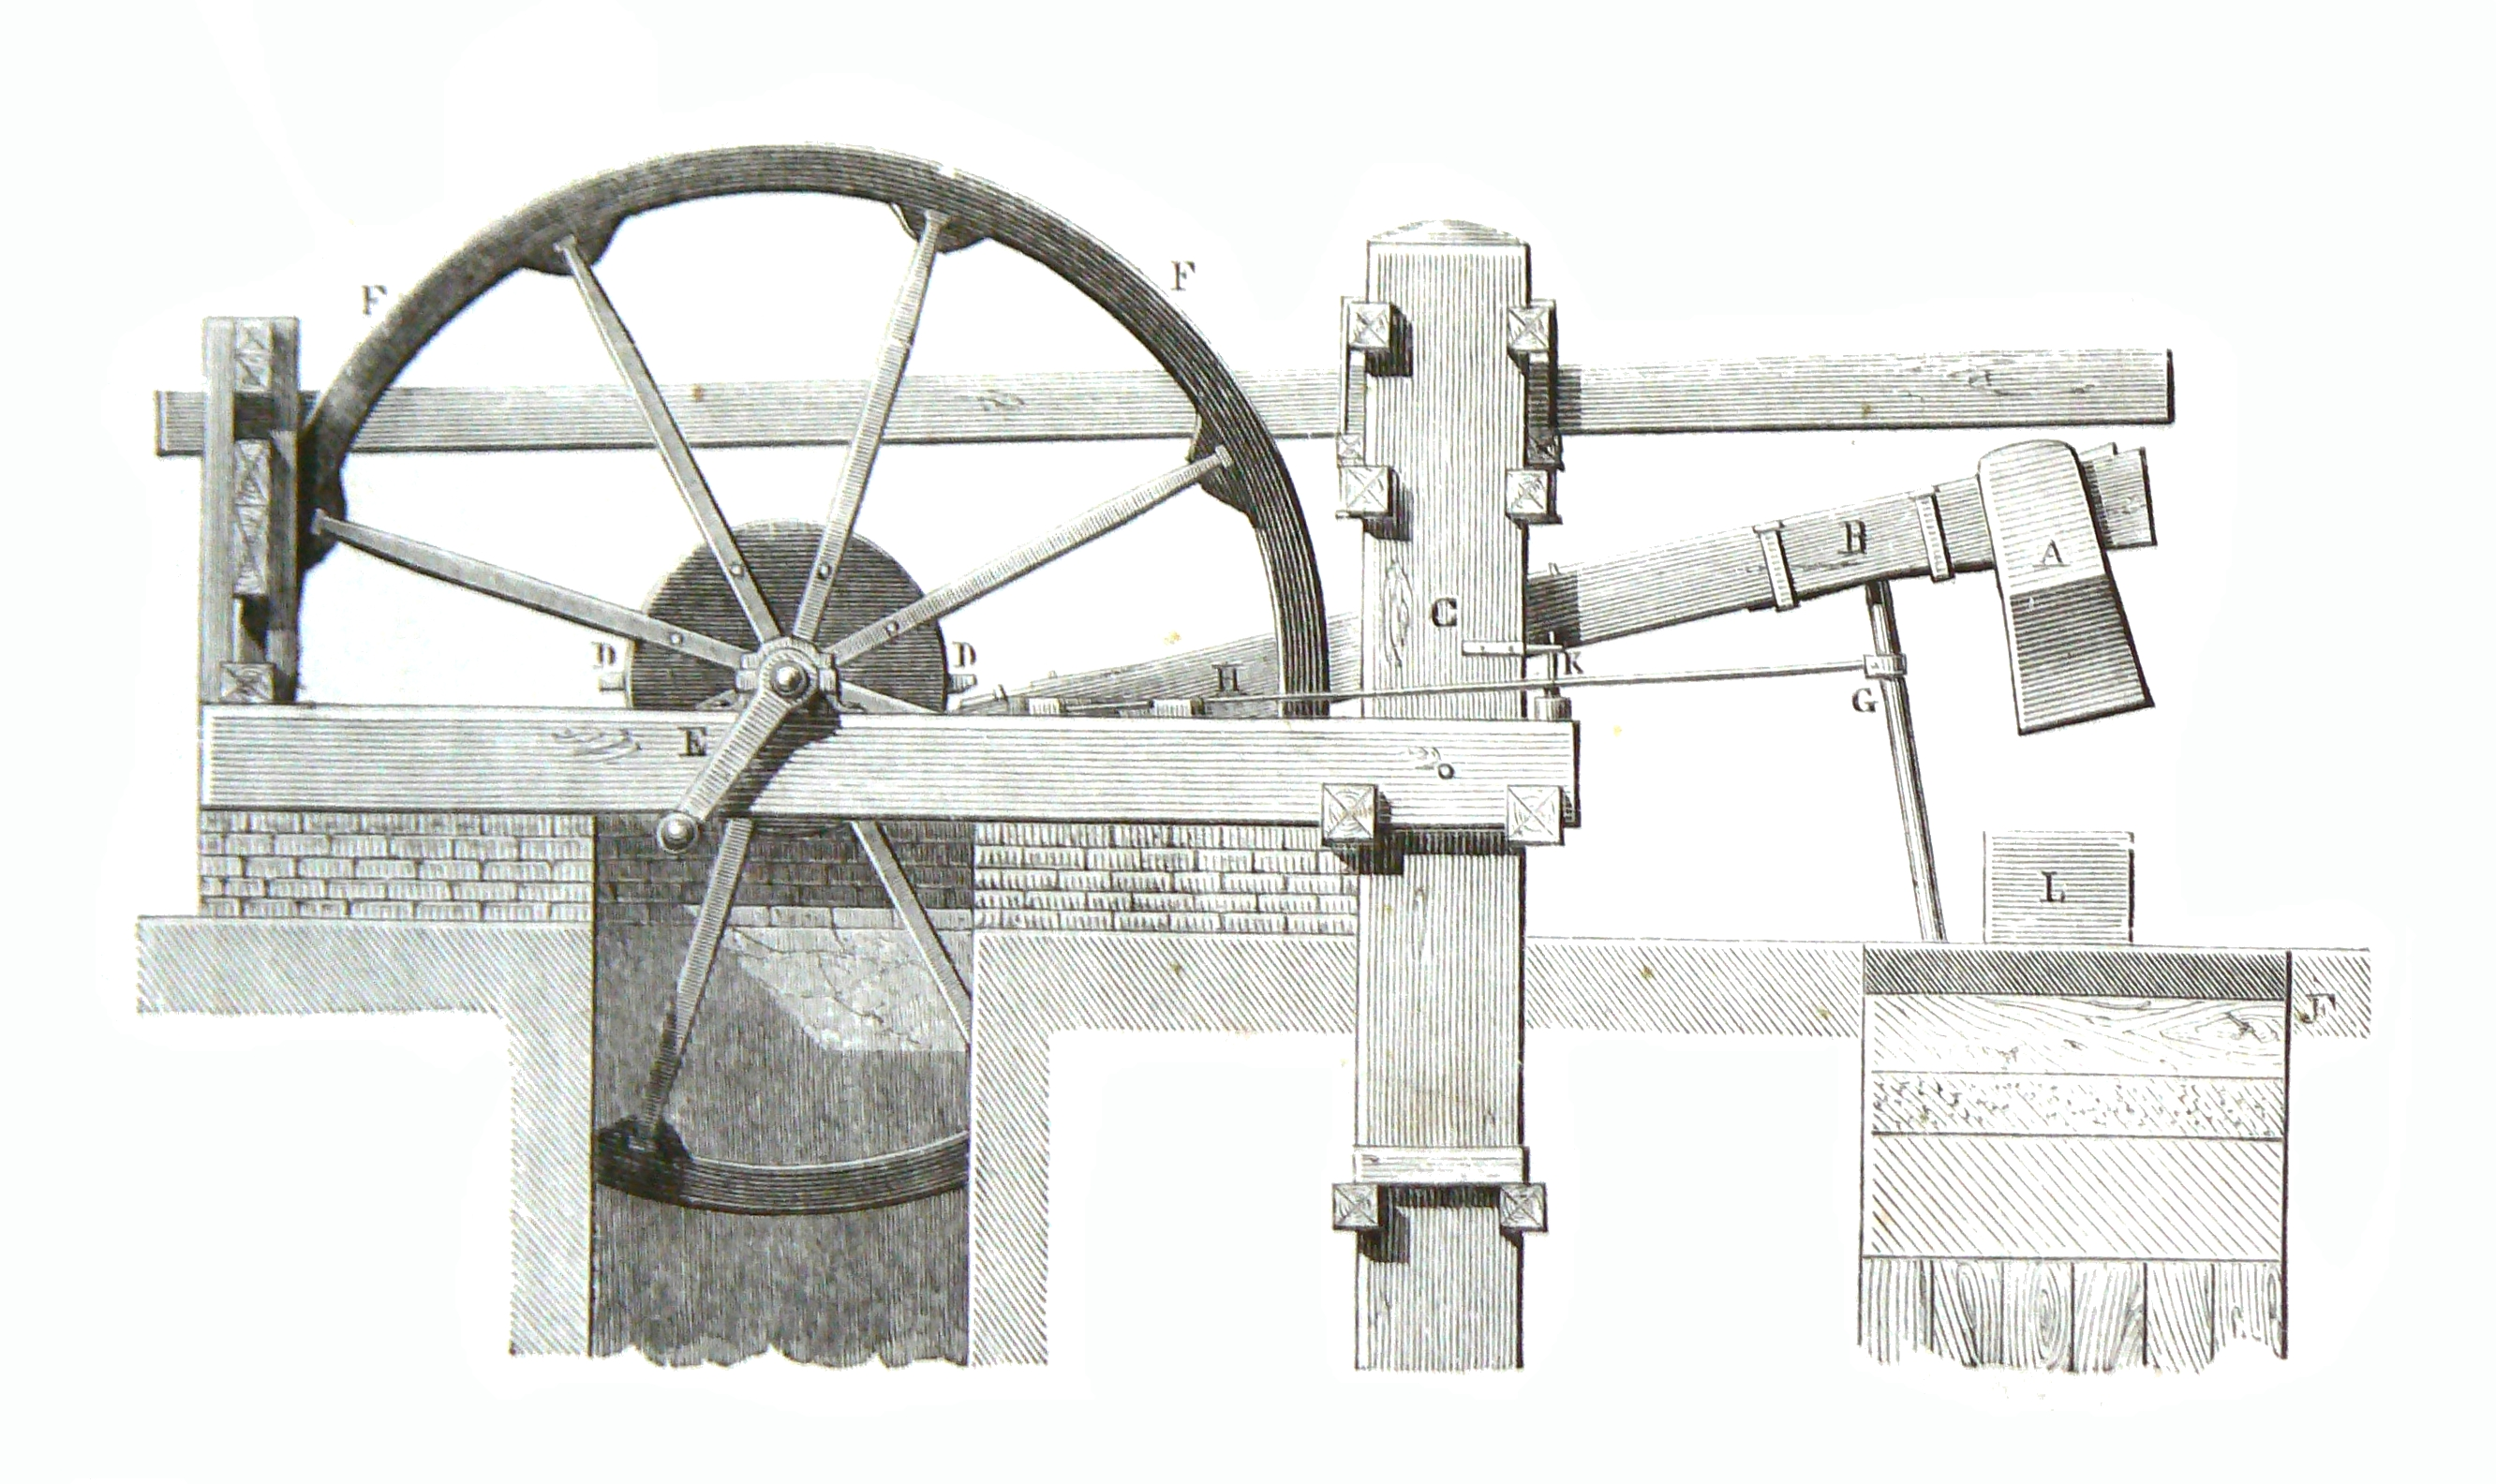
\includegraphics[width=0.8\linewidth]{blacksmith.jpg}
\end{figure}

{\small source https://commons.wikimedia.org/w/index.php?curid=1520727}

\end{center}
\end{frame}

%%%%%%%%%%%%%%%%%%%%%%%%%%%%%

\begin{frame}{Current definition: ISO 8373:2012(en)}
\begin{center}
\textbf{\large  Robots and robotic devices\\[4pt]}

Actuated mechanism (re-)programmable in two or more axes with a degree of autonomy, moving within its environment, to perform intended tasks.

\end{center}
\end{frame}

%%%%%%%%%%%%%%%%%%%%%%%%%%%%%

\begin{frame}{First manipulator - Unimate}
\begin{center}
\begin{minipage}{0.49\linewidth}
\begin{center}
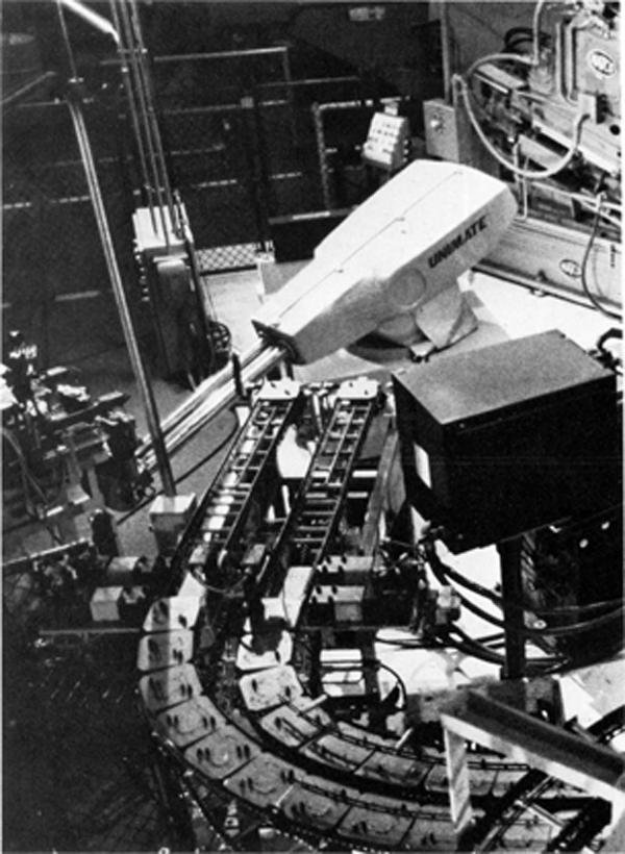
\includegraphics[width=0.8\linewidth]{unimate.png}
\end{center}
\end{minipage}
\hfill
\begin{minipage}{0.49\linewidth}
\begin{itemize}
\item Developed in the 50's
\item Industrialized in 61
\item Only predefined tasks
\end{itemize}
\end{minipage}

\end{center}
\end{frame}

%%%%%%%%%%%%%%%%%%%%%%%%%%%%%

\begin{frame}{First mobile autonomous robot - Shakey}
\begin{center}
\begin{minipage}{0.49\linewidth}
\begin{center}
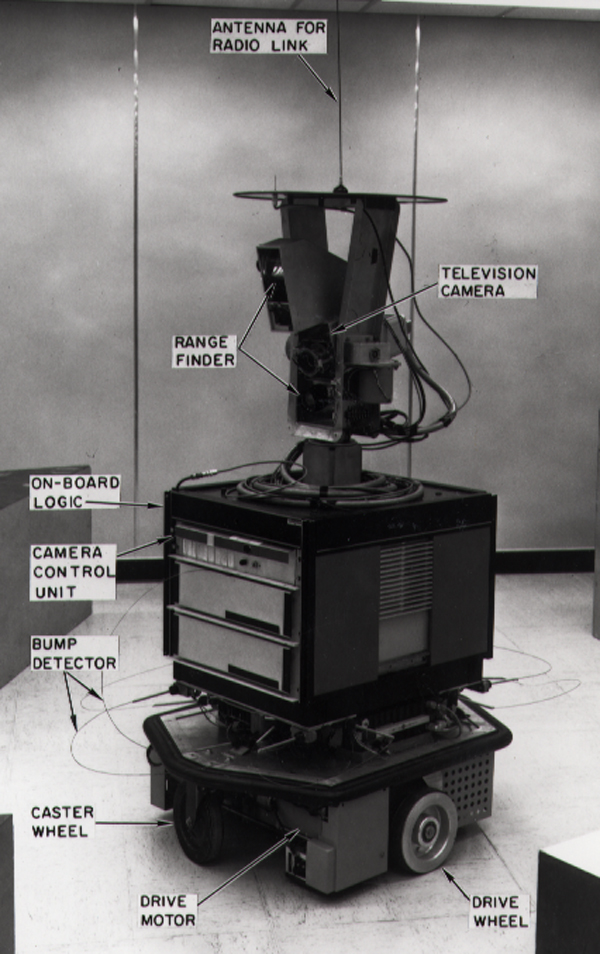
\includegraphics[width=0.8\linewidth]{SRI_Shakey_with_callouts.jpg}
\end{center}
\end{minipage}
\hfill
\begin{minipage}{0.49\linewidth}
\begin{itemize}
\item Developed from 66 to 72
\item Object recognition
\item Path and task planning
\end{itemize}
\end{minipage}

\end{center}
\end{frame}

%%%%%%%%%%%%%%%%%%%%%%%%%%%%%

\begin{frame}{First mobile autonomous robot - Shakey}
\begin{center}
\begin{minipage}{0.49\linewidth}
\begin{center}
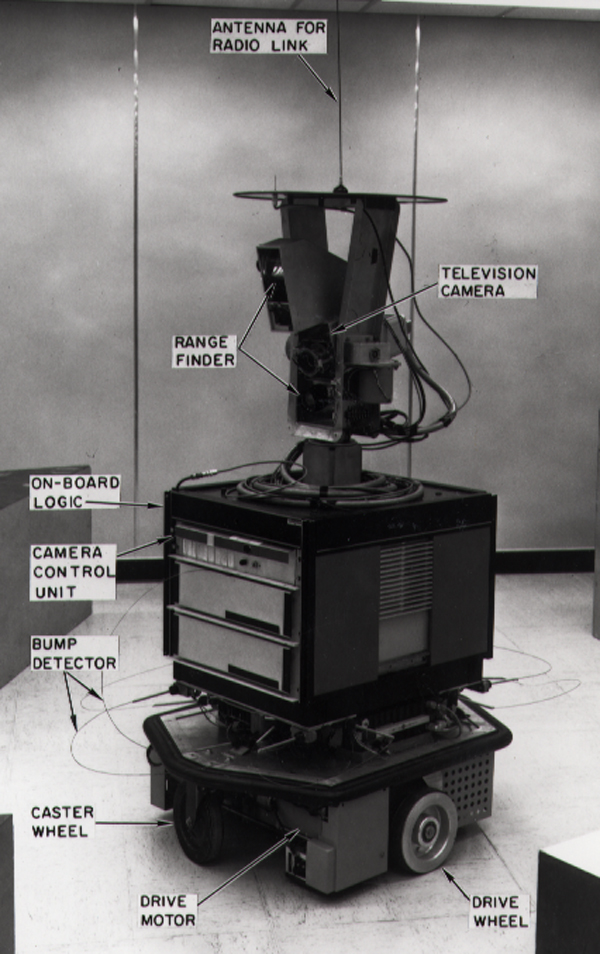
\includegraphics[width=0.8\linewidth]{SRI_Shakey_with_callouts.jpg}
\end{center}
\end{minipage}
\hfill
\begin{minipage}{0.49\linewidth}
\begin{itemize}
\item Developed from 66 to 72
\item Object recognition
\item Path and task planning
\end{itemize}
\end{minipage}

\end{center}
\end{frame}

%%%%%%%%%%%%%%%%%%%%%%%%%%%%%

\begin{frame}{Autonomous robots state of the art - Atlas}
\begin{center}
\only<1>{
	\begin{minipage}{0.49\linewidth}
	\begin{center}
	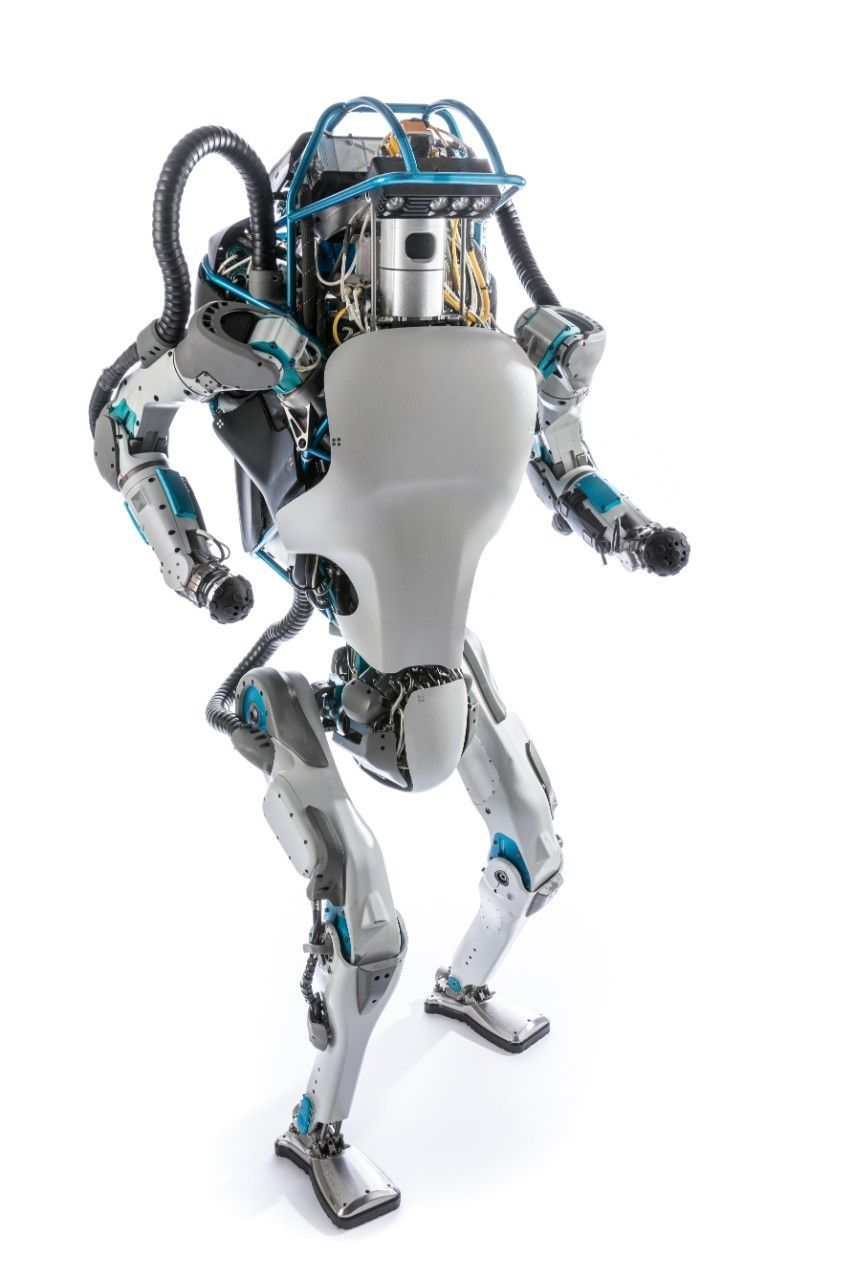
\includegraphics[width=0.8\linewidth]{Atlas_intro.jpg}
	\end{center}
	\end{minipage}
	\hfill
	\begin{minipage}{0.49\linewidth}
	\begin{itemize}
	\item Humanoid robot developed by Boston dynamics
	\item Largely autonomous
	\item Path and task planning
	\end{itemize}
	\end{minipage}
}
\only<2>{
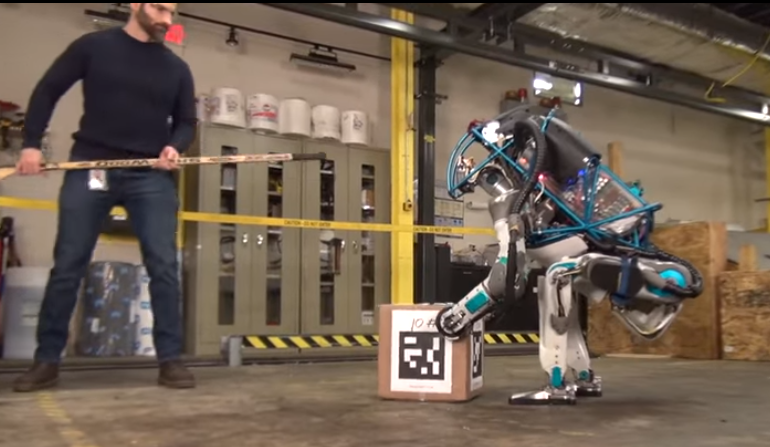
\includegraphics[width=0.99\linewidth]{Atlas_trying.png}
}
\only<3>{
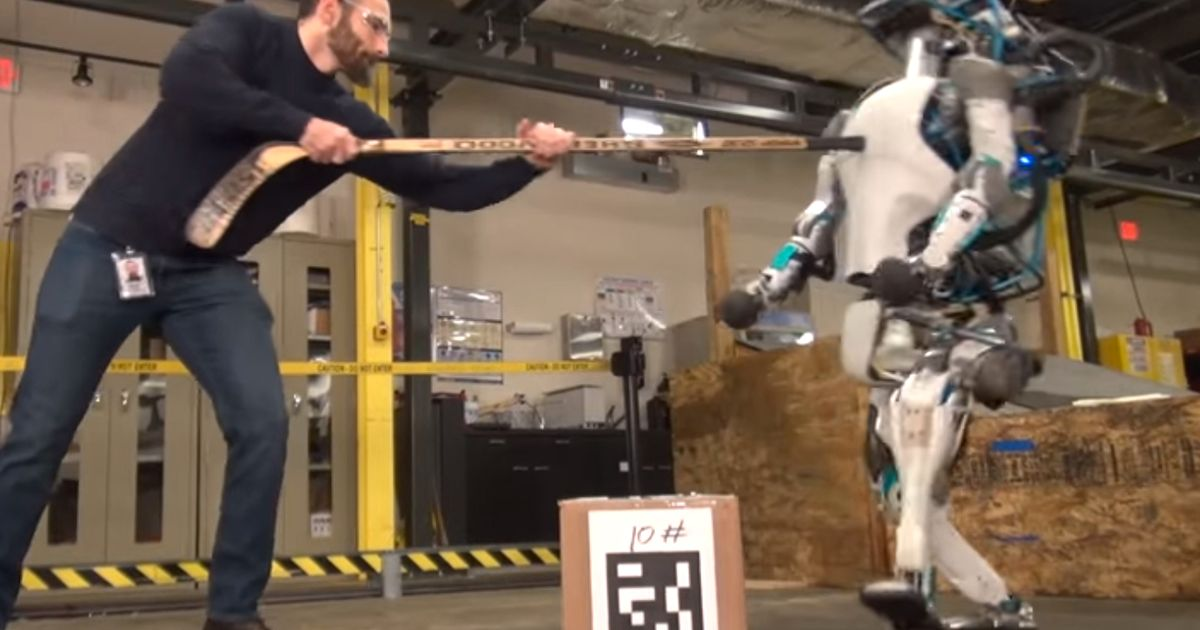
\includegraphics[width=0.99\linewidth]{Atlas_push.jpg}
}
\only<4>{
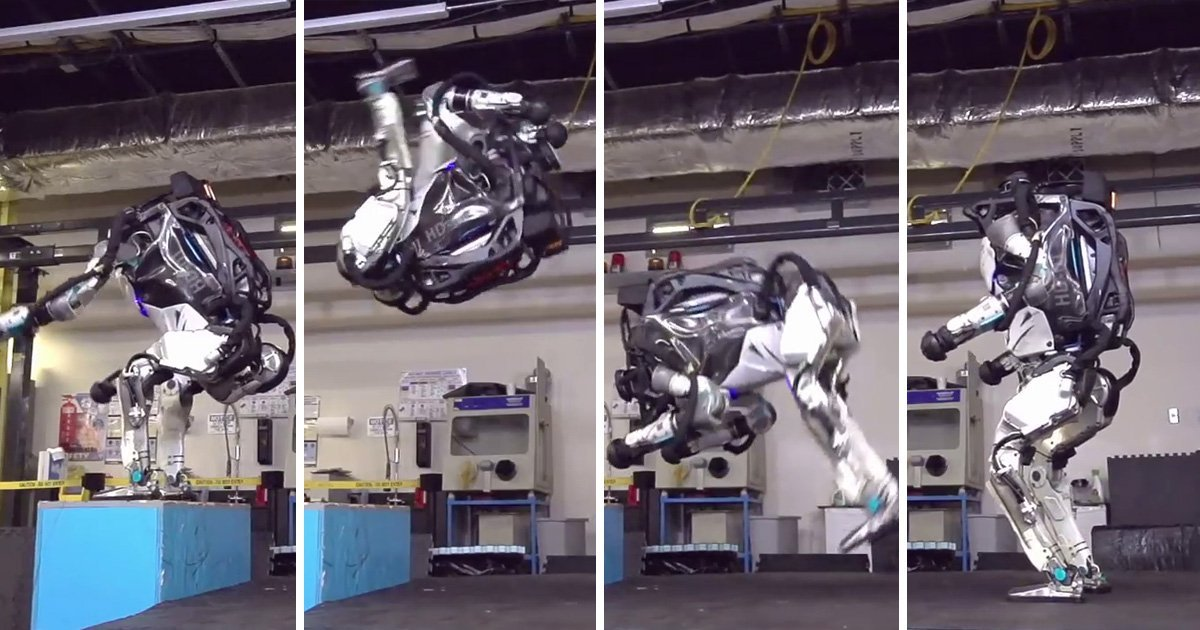
\includegraphics[width=0.99\linewidth]{Atlas_backflip.jpg}
}
\end{center}
\end{frame}

%%%%%%%%%%%%%%%%%%%%%%%%%%%%%%%%%%%%%%%%%%%%%%%%%%%%%%%%%%
\section{The control theoretic perspective}
%%%%%%%%%%%%%%%%%%%%%%%%%%%%%
\begin{frame}{Robot control - Overview}
\begin{center}
\only<1>{
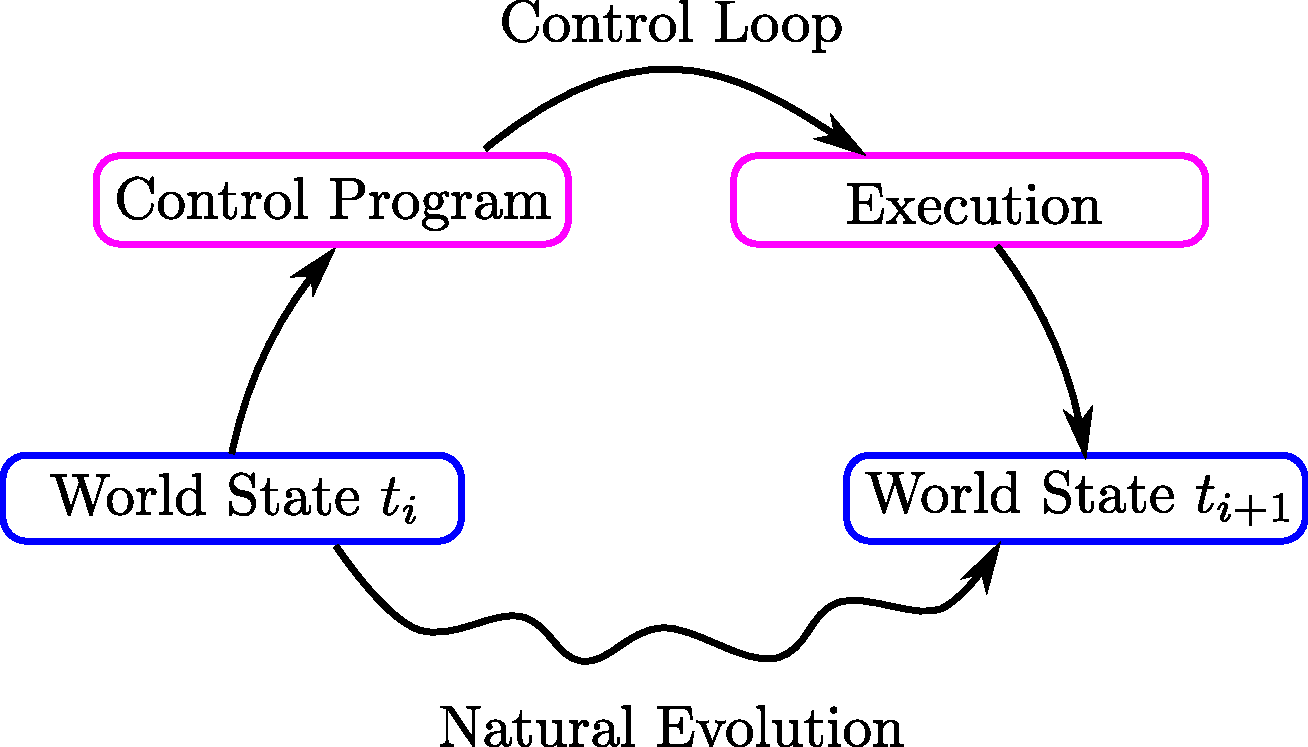
\includegraphics[width=0.7\linewidth]{control1.pdf}
}
\only<2>{
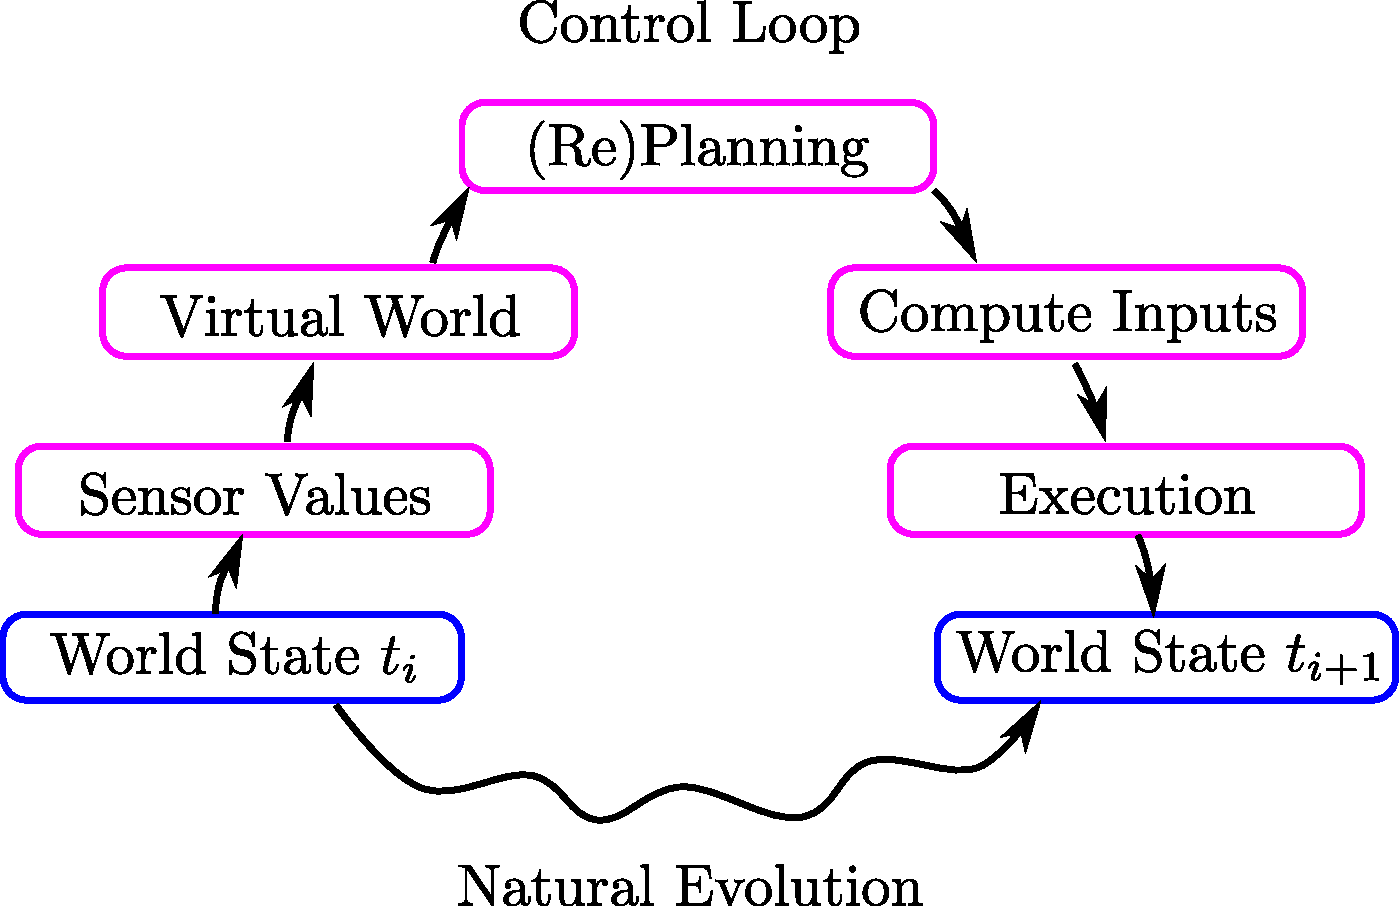
\includegraphics[width=0.85\linewidth]{control2.pdf}
}
\end{center}
\end{frame}
%%%%%%%%%%%%%%%%%%%%%%%%%%%%%
\begin{frame}{Control theory - Goal}
\begin{center}
{\large Control theory seeks means to generate control signals or inputs such that the state evolves in a desired way. }
\end{center}
\end{frame}
%%%%%%%%%%%%%%%%%%%%%%%%%%%%%
\begin{frame}{Control theory - Realization I}
\begin{center}
	\vspace{-6pt}
    \textbf{\Large Centrifugal governor\\[4pt]}
    \def\svgwidth{.5\linewidth}
    \input{regulator.pdf_tex}
    \visible<2>{
    \begin{minipage}{0.49\linewidth}
    \begin{center}
        opening angle depends on current speed
    \end{center}
    \end{minipage}
    \begin{minipage}{0.49\linewidth}
    \begin{center}
        negative feedback between opening angle and input power
    \end{center}
    \end{minipage}
    }
\end{center}
\end{frame}
%%%%%%%%%%%%%%%%%%%%%%%%%%%%%
\begin{frame}{Control theory - Concepts I}
A robot from a control theoretic perspective looks like this:
\begin{align*}
    \xd &= f(\x) + g_{\uv}(\x, \uv) + g_{{\omega_{\x}}}(\x, \omega_{\x})  \\
    \y &= h(\x, \omega_{\y})
\end{align*}
\visible<1->{
    \begin{columns}
    \begin{column}{0.5\linewidth}
        $\x$ : system state \\
        $\y$ : output state \\
        $\omega_{\x}$ : perturbations \\
        $\omega_{\y}$ : (measurement) noise
    \end{column}
    \begin{column}{0.5\linewidth}
        $f,\ g$ : system and input dynamics \\
        $\uv$ : control input \\
        $g_{{\omega_{\x}}}$ : perturbation dynamics
    \end{column}
    \end{columns}
}
\end{frame}
%%%%%%%%%%%%%%%%%%%%%%%%%%%%%
\begin{frame}{Control theory - Concepts II}
\begin{center}
\textbf{\Large Formalizing ``in a desired way''}\\[12pt]
\begin{minipage}{\linewidth}
\begin{minipage}[t]{0.49\linewidth}
	\begin{center}
	\textbf{\large Trajectory generation: }\\[4pt]
	compute a feasible trajectory
	\end{center}	
	\vfill
\end{minipage}
\hfill
\begin{minipage}[t]{0.49\linewidth}
	\begin{center}
	\textbf{\large Stabilization: }\\[4pt]
	reject perturbations and make the control ``robust''
	\end{center}
	\vfill
\end{minipage}
\visible<2>{
\begin{center}
\textbf{\large Classification of the dynamics:\\[4pt] }
\begin{minipage}[c]{\linewidth}
	\textbullet nonlinear \hfill \textbullet polynomial \hfill \textbullet linear \hfill
\end{minipage}
\end{center}
}
\end{minipage}
\end{center}
\end{frame}
%%%%%%%%%%%%%%%%%%%%%%%%%%%%%
\begin{frame}{Trajectory generation - Dubins' car}
\begin{center}
Simplified car dynamics:\\
constant forward velocity, minimal turning radius
\only<1>{
\begin{figure}
	\def\svgwidth{\linewidth}
	\input{dubins.pdf_tex}
\end{figure}
It can be shown that the ideal (shortest) trajectory between two configurations contains only straight lines and circle segments with minimal radius.
}

\only<2>{
\begin{figure}
	\def\svgwidth{.6\linewidth}
	\input{dubins_2_0.pdf_tex}
\end{figure}
By allowing for more expressive behaviour (obstacles), the problem becomes (drastically) more complicated.
}
%https://en.wikipedia.org/wiki/Dubins_path
%Johnson, H. H "An application of the maximum principle to the geometry of plane curves", Proceedings of the American Mathematical Society, 44(2):432- 435, 1974.
%Boissonat, J.D.; A. Cerezo; K. Leblond (May 1992). "Shortest Paths of Bounded Curvature in the Plane" (PDF). Proceedings of the IEEE International Conference on Robotics and Automation. 3. Piscataway, NJ. pp. 2315–2320. doi:10.1109/ROBOT.1992.220117.
\end{center}
\end{frame}
%%%%%%%%%%%%%%%%%%%%%%%%%%%%%
\begin{frame}{Trajectory generation - Randomized planning}
\only<1>{
\begin{figure}
	\def\svgwidth{\linewidth}
	\input{planning_0.pdf_tex}
\end{figure}
}
\only<2>{
\begin{figure}
	\def\svgwidth{\linewidth}
	\input{planning_1.pdf_tex}
\end{figure}
}
\only<3>{
\begin{figure}
	\def\svgwidth{.8\linewidth}
	\input{planning_2.pdf_tex}
\end{figure}
}
\only<4>{
\begin{figure}
	\def\svgwidth{.8\linewidth}
	\input{planning_3.pdf_tex}
\end{figure}
}
\only<5>{
\begin{figure}
	\def\svgwidth{.8\linewidth}
	\input{planning_4.pdf_tex}
\end{figure}
}
\end{frame}
%%%%%%%%%%%%%%%%%%%%%%%%%%%%%
\begin{frame}{Trajectory stabilization}
\begin{center}
Trajectory generators give us a reference trajectory and in an ideal world we could simply replay the inputs $\uv(t)$.\\
\visible<2->{This is called open-loop control\\[4pt]}
\visible<3->{Sadly the world isn't perfect: modelling errors, noise, friction, ...}
\visible<4->{
\begin{figure}
	\def\svgwidth{.8\linewidth}
	\input{trajectory_stab_1.pdf_tex}	
\end{figure}
Compute a control law $g(\delta\x)$ s.t. the system trajectory converges to its reference
}
\end{center}
\end{frame}
%%%%%%%%%%%%%%%%%%%%%%%%%%%%%
\begin{frame}{Trajectory stabilization - optimal control}
% https://stanford.edu/class/ee363/lectures/dlqr.pdf
% https://ocw.mit.edu/courses/mechanical-engineering/2-154-maneuvering-and-control-of-surface-and-underwater-vehicles-13-49-fall-2004/lecture-notes/lec19.pdf
\begin{center}
Consider the discrete-time linear system:
\begin{equation*}
\x_i = A.\x_{i-1} + B.\uv_{i-1}
\end{equation*}
and optimality defined by the cost function
\begin{equation}
J(\x_0) = \sum_{{i=0}}^{{N-1}}\left(\xT_i.Q.\x_i + \tp{\uv}_i.R.\uv_i\right) + \xT_N.Q.\x_N
\end{equation}
Possible methods to obtain the Linear Quadratic Regulator (LQR):\\[6pt]
\begin{minipage}[c]{0.5\linewidth}
\begin{itemize}
\item via Least-Squares
\item via Dynamic Programming
\item via Convex Optimization
\end{itemize}
\end{minipage}
\end{center}
\end{frame}

%%%%%%%%%%%%%%%%%%%%%%%%%%%%%
\begin{frame}{Optimal control - Dynamic Programming}
\begin{center}
A solution can be found using dynamic programming and iterating from end to start.\\[4pt]

The final cost is ``fixed'': $J(\x_N) = \xT_N.Q.\x_N$ \\[4pt]
\visible<2->{
	The cost for $i=N-1$ is:\\[4pt]
	$J(\x_{N-1}) = \xT_{N-1}.Q.\x_{N-1} + \tp{\uv}_{N-1}.R.\uv_{N-1} + \xT_N.Q.\x_N$\\
	and moreover $\x_i = A.\x_{i-1} + B.\uv_{i-1}$
} 
\visible<3->{ so we get:\\[4pt]
$J(\x_{N-1}) = \xT_{N-1}.Q.\x_{N-1} + \tp{\uv}_{N-1}.R.\uv_{N-1} + J(A.\x_{i-1} + B.\uv_{i-1})$\\
}

\end{center}
\end{frame}

%%%%%%%%%%%%%%%%%%%%%%%%%%%%%

\begin{frame}{Optimal control - Dynamic Programming}
\begin{center}

This means that we can solve the problem by recursively solving :\\[4pt]
$\uv_{N-1} = \argmin{\uv}\ \tp{\uv}.R.\uv + J(A.\x_{i-1} + B.\uv)$\\[2pt]

\visible<1->{
	and after some linear algebra one can find an optimal linear feedback matrix:\\[4pt]
	$\uv_{N-1} = K_{N-1}.\x$ \\[2pt]
	So we have established a time-dependent linear control law that is optimal in the sense of the cost function.
}

\end{center}
\end{frame}

%%%%%%%%%%%%%%%%%%%%%%%%%%%%%

\begin{frame}{Optimal control - 2d linear system}
\begin{center}
\only<1>{
Mass-spring-damper model
\begin{equation}
\xd = \begin{pmatrix} \dot{x} \\ \ddot{x} \end{pmatrix} = \begin{bmatrix} 0. & 1. \\ -0.5 & -0.15 \end{bmatrix} . \begin{pmatrix} x \\ \dot{x} \end{pmatrix}
\end{equation}
with 
\begin{equation}
Q = \begin{bmatrix} 1. & 0. \\ 0. & 1. \end{bmatrix} \ \ \ \ R = \begin{bmatrix} 1. \end{bmatrix}
\end{equation}
}
\only<2>{
%% Creator: Matplotlib, PGF backend
%%
%% To include the figure in your LaTeX document, write
%%   \input{<filename>.pgf}
%%
%% Make sure the required packages are loaded in your preamble
%%   \usepackage{pgf}
%%
%% Figures using additional raster images can only be included by \input if
%% they are in the same directory as the main LaTeX file. For loading figures
%% from other directories you can use the `import` package
%%   \usepackage{import}
%% and then include the figures with
%%   \import{<path to file>}{<filename>.pgf}
%%
%% Matplotlib used the following preamble
%%   \usepackage{units}
%%   \usepackage{metalogo}
%%   \usepackage{unicode-math}
%%   \setmathfont{xits-math.otf}
%%   \setmainfont{DejaVu Serif}
%%   \usepackage{fontspec}
%%
\begingroup%
\makeatletter%
\begin{pgfpicture}%
\pgfpathrectangle{\pgfpointorigin}{\pgfqpoint{4.000000in}{2.800000in}}%
\pgfusepath{use as bounding box, clip}%
\begin{pgfscope}%
\pgfsetbuttcap%
\pgfsetmiterjoin%
\definecolor{currentfill}{rgb}{1.000000,1.000000,1.000000}%
\pgfsetfillcolor{currentfill}%
\pgfsetlinewidth{0.000000pt}%
\definecolor{currentstroke}{rgb}{1.000000,1.000000,1.000000}%
\pgfsetstrokecolor{currentstroke}%
\pgfsetdash{}{0pt}%
\pgfpathmoveto{\pgfqpoint{0.000000in}{0.000000in}}%
\pgfpathlineto{\pgfqpoint{4.000000in}{0.000000in}}%
\pgfpathlineto{\pgfqpoint{4.000000in}{2.800000in}}%
\pgfpathlineto{\pgfqpoint{0.000000in}{2.800000in}}%
\pgfpathclose%
\pgfusepath{fill}%
\end{pgfscope}%
\begin{pgfscope}%
\pgfsetbuttcap%
\pgfsetmiterjoin%
\definecolor{currentfill}{rgb}{1.000000,1.000000,1.000000}%
\pgfsetfillcolor{currentfill}%
\pgfsetlinewidth{0.000000pt}%
\definecolor{currentstroke}{rgb}{0.000000,0.000000,0.000000}%
\pgfsetstrokecolor{currentstroke}%
\pgfsetstrokeopacity{0.000000}%
\pgfsetdash{}{0pt}%
\pgfpathmoveto{\pgfqpoint{0.396851in}{1.998950in}}%
\pgfpathlineto{\pgfqpoint{3.820000in}{1.998950in}}%
\pgfpathlineto{\pgfqpoint{3.820000in}{2.620000in}}%
\pgfpathlineto{\pgfqpoint{0.396851in}{2.620000in}}%
\pgfpathclose%
\pgfusepath{fill}%
\end{pgfscope}%
\begin{pgfscope}%
\definecolor{textcolor}{rgb}{0.000000,0.000000,0.000000}%
\pgfsetstrokecolor{textcolor}%
\pgfsetfillcolor{textcolor}%
\pgftext[x=0.341295in,y=2.309475in,,bottom,rotate=90.000000]{\color{textcolor}\rmfamily\fontsize{12.000000}{14.400000}\selectfont \(\displaystyle x\)}%
\end{pgfscope}%
\begin{pgfscope}%
\pgfpathrectangle{\pgfqpoint{0.396851in}{1.998950in}}{\pgfqpoint{3.423149in}{0.621050in}}%
\pgfusepath{clip}%
\pgfsetrectcap%
\pgfsetroundjoin%
\pgfsetlinewidth{1.505625pt}%
\definecolor{currentstroke}{rgb}{0.000000,0.000000,1.000000}%
\pgfsetstrokecolor{currentstroke}%
\pgfsetdash{}{0pt}%
\pgfpathmoveto{\pgfqpoint{0.552449in}{2.419172in}}%
\pgfpathlineto{\pgfqpoint{0.716236in}{2.419172in}}%
\pgfpathlineto{\pgfqpoint{0.716236in}{2.419172in}}%
\pgfpathlineto{\pgfqpoint{0.880023in}{2.419172in}}%
\pgfpathlineto{\pgfqpoint{0.880023in}{2.419172in}}%
\pgfpathlineto{\pgfqpoint{1.043810in}{2.419172in}}%
\pgfpathlineto{\pgfqpoint{1.043810in}{2.419172in}}%
\pgfpathlineto{\pgfqpoint{1.207597in}{2.419172in}}%
\pgfpathlineto{\pgfqpoint{1.207597in}{2.419172in}}%
\pgfpathlineto{\pgfqpoint{1.371384in}{2.419172in}}%
\pgfpathlineto{\pgfqpoint{1.371384in}{2.419172in}}%
\pgfpathlineto{\pgfqpoint{1.535171in}{2.419172in}}%
\pgfpathlineto{\pgfqpoint{1.535171in}{2.419172in}}%
\pgfpathlineto{\pgfqpoint{1.698958in}{2.419172in}}%
\pgfpathlineto{\pgfqpoint{1.698958in}{2.419172in}}%
\pgfpathlineto{\pgfqpoint{1.862745in}{2.419172in}}%
\pgfpathlineto{\pgfqpoint{1.862745in}{2.419172in}}%
\pgfpathlineto{\pgfqpoint{2.026532in}{2.419172in}}%
\pgfpathlineto{\pgfqpoint{2.026532in}{2.419172in}}%
\pgfpathlineto{\pgfqpoint{2.190319in}{2.419172in}}%
\pgfpathlineto{\pgfqpoint{2.190319in}{2.419172in}}%
\pgfpathlineto{\pgfqpoint{2.354106in}{2.419172in}}%
\pgfpathlineto{\pgfqpoint{2.354106in}{2.419172in}}%
\pgfpathlineto{\pgfqpoint{2.517893in}{2.419172in}}%
\pgfpathlineto{\pgfqpoint{2.517893in}{2.419172in}}%
\pgfpathlineto{\pgfqpoint{2.681680in}{2.419172in}}%
\pgfpathlineto{\pgfqpoint{2.681680in}{2.419172in}}%
\pgfpathlineto{\pgfqpoint{2.845467in}{2.419172in}}%
\pgfpathlineto{\pgfqpoint{2.845467in}{2.419172in}}%
\pgfpathlineto{\pgfqpoint{3.009254in}{2.419172in}}%
\pgfpathlineto{\pgfqpoint{3.009254in}{2.419172in}}%
\pgfpathlineto{\pgfqpoint{3.173041in}{2.419172in}}%
\pgfpathlineto{\pgfqpoint{3.173041in}{2.419172in}}%
\pgfpathlineto{\pgfqpoint{3.336828in}{2.419172in}}%
\pgfpathlineto{\pgfqpoint{3.336828in}{2.419172in}}%
\pgfpathlineto{\pgfqpoint{3.500615in}{2.419172in}}%
\pgfpathlineto{\pgfqpoint{3.500615in}{2.419172in}}%
\pgfpathlineto{\pgfqpoint{3.664402in}{2.419172in}}%
\pgfpathlineto{\pgfqpoint{3.664402in}{2.419172in}}%
\pgfusepath{stroke}%
\end{pgfscope}%
\begin{pgfscope}%
\pgfpathrectangle{\pgfqpoint{0.396851in}{1.998950in}}{\pgfqpoint{3.423149in}{0.621050in}}%
\pgfusepath{clip}%
\pgfsetrectcap%
\pgfsetroundjoin%
\pgfsetlinewidth{1.505625pt}%
\definecolor{currentstroke}{rgb}{0.000000,0.000000,0.000000}%
\pgfsetstrokecolor{currentstroke}%
\pgfsetdash{}{0pt}%
\pgfpathmoveto{\pgfqpoint{0.552449in}{2.103002in}}%
\pgfpathlineto{\pgfqpoint{0.716236in}{2.103002in}}%
\pgfpathlineto{\pgfqpoint{0.716236in}{2.027180in}}%
\pgfpathlineto{\pgfqpoint{0.880023in}{2.027180in}}%
\pgfpathlineto{\pgfqpoint{0.880023in}{2.143325in}}%
\pgfpathlineto{\pgfqpoint{1.043810in}{2.143325in}}%
\pgfpathlineto{\pgfqpoint{1.043810in}{2.342590in}}%
\pgfpathlineto{\pgfqpoint{1.207597in}{2.342590in}}%
\pgfpathlineto{\pgfqpoint{1.207597in}{2.513749in}}%
\pgfpathlineto{\pgfqpoint{1.371384in}{2.513749in}}%
\pgfpathlineto{\pgfqpoint{1.371384in}{2.591770in}}%
\pgfpathlineto{\pgfqpoint{1.535171in}{2.591770in}}%
\pgfpathlineto{\pgfqpoint{1.535171in}{2.571614in}}%
\pgfpathlineto{\pgfqpoint{1.698958in}{2.571614in}}%
\pgfpathlineto{\pgfqpoint{1.698958in}{2.491997in}}%
\pgfpathlineto{\pgfqpoint{1.862745in}{2.491997in}}%
\pgfpathlineto{\pgfqpoint{1.862745in}{2.405333in}}%
\pgfpathlineto{\pgfqpoint{2.026532in}{2.405333in}}%
\pgfpathlineto{\pgfqpoint{2.026532in}{2.351027in}}%
\pgfpathlineto{\pgfqpoint{2.190319in}{2.351027in}}%
\pgfpathlineto{\pgfqpoint{2.190319in}{2.342559in}}%
\pgfpathlineto{\pgfqpoint{2.354106in}{2.342559in}}%
\pgfpathlineto{\pgfqpoint{2.354106in}{2.369656in}}%
\pgfpathlineto{\pgfqpoint{2.517893in}{2.369656in}}%
\pgfpathlineto{\pgfqpoint{2.517893in}{2.409958in}}%
\pgfpathlineto{\pgfqpoint{2.681680in}{2.409958in}}%
\pgfpathlineto{\pgfqpoint{2.681680in}{2.442251in}}%
\pgfpathlineto{\pgfqpoint{2.845467in}{2.442251in}}%
\pgfpathlineto{\pgfqpoint{2.845467in}{2.455112in}}%
\pgfpathlineto{\pgfqpoint{3.009254in}{2.455112in}}%
\pgfpathlineto{\pgfqpoint{3.009254in}{2.448742in}}%
\pgfpathlineto{\pgfqpoint{3.173041in}{2.448742in}}%
\pgfpathlineto{\pgfqpoint{3.173041in}{2.431344in}}%
\pgfpathlineto{\pgfqpoint{3.336828in}{2.431344in}}%
\pgfpathlineto{\pgfqpoint{3.336828in}{2.413313in}}%
\pgfpathlineto{\pgfqpoint{3.500615in}{2.413313in}}%
\pgfpathlineto{\pgfqpoint{3.500615in}{2.402372in}}%
\pgfpathlineto{\pgfqpoint{3.664402in}{2.402372in}}%
\pgfpathlineto{\pgfqpoint{3.664402in}{2.401319in}}%
\pgfusepath{stroke}%
\end{pgfscope}%
\begin{pgfscope}%
\pgfsetrectcap%
\pgfsetmiterjoin%
\pgfsetlinewidth{0.803000pt}%
\definecolor{currentstroke}{rgb}{0.000000,0.000000,0.000000}%
\pgfsetstrokecolor{currentstroke}%
\pgfsetdash{}{0pt}%
\pgfpathmoveto{\pgfqpoint{0.396851in}{1.998950in}}%
\pgfpathlineto{\pgfqpoint{0.396851in}{2.620000in}}%
\pgfusepath{stroke}%
\end{pgfscope}%
\begin{pgfscope}%
\pgfsetrectcap%
\pgfsetmiterjoin%
\pgfsetlinewidth{0.803000pt}%
\definecolor{currentstroke}{rgb}{0.000000,0.000000,0.000000}%
\pgfsetstrokecolor{currentstroke}%
\pgfsetdash{}{0pt}%
\pgfpathmoveto{\pgfqpoint{3.820000in}{1.998950in}}%
\pgfpathlineto{\pgfqpoint{3.820000in}{2.620000in}}%
\pgfusepath{stroke}%
\end{pgfscope}%
\begin{pgfscope}%
\pgfsetrectcap%
\pgfsetmiterjoin%
\pgfsetlinewidth{0.803000pt}%
\definecolor{currentstroke}{rgb}{0.000000,0.000000,0.000000}%
\pgfsetstrokecolor{currentstroke}%
\pgfsetdash{}{0pt}%
\pgfpathmoveto{\pgfqpoint{0.396851in}{1.998950in}}%
\pgfpathlineto{\pgfqpoint{3.820000in}{1.998950in}}%
\pgfusepath{stroke}%
\end{pgfscope}%
\begin{pgfscope}%
\pgfsetrectcap%
\pgfsetmiterjoin%
\pgfsetlinewidth{0.803000pt}%
\definecolor{currentstroke}{rgb}{0.000000,0.000000,0.000000}%
\pgfsetstrokecolor{currentstroke}%
\pgfsetdash{}{0pt}%
\pgfpathmoveto{\pgfqpoint{0.396851in}{2.620000in}}%
\pgfpathlineto{\pgfqpoint{3.820000in}{2.620000in}}%
\pgfusepath{stroke}%
\end{pgfscope}%
\begin{pgfscope}%
\pgfsetbuttcap%
\pgfsetmiterjoin%
\definecolor{currentfill}{rgb}{1.000000,1.000000,1.000000}%
\pgfsetfillcolor{currentfill}%
\pgfsetlinewidth{0.000000pt}%
\definecolor{currentstroke}{rgb}{0.000000,0.000000,0.000000}%
\pgfsetstrokecolor{currentstroke}%
\pgfsetstrokeopacity{0.000000}%
\pgfsetdash{}{0pt}%
\pgfpathmoveto{\pgfqpoint{0.396851in}{1.197901in}}%
\pgfpathlineto{\pgfqpoint{3.820000in}{1.197901in}}%
\pgfpathlineto{\pgfqpoint{3.820000in}{1.818950in}}%
\pgfpathlineto{\pgfqpoint{0.396851in}{1.818950in}}%
\pgfpathclose%
\pgfusepath{fill}%
\end{pgfscope}%
\begin{pgfscope}%
\definecolor{textcolor}{rgb}{0.000000,0.000000,0.000000}%
\pgfsetstrokecolor{textcolor}%
\pgfsetfillcolor{textcolor}%
\pgftext[x=0.341295in,y=1.508425in,,bottom,rotate=90.000000]{\color{textcolor}\rmfamily\fontsize{12.000000}{14.400000}\selectfont \(\displaystyle \dot{x}\)}%
\end{pgfscope}%
\begin{pgfscope}%
\pgfpathrectangle{\pgfqpoint{0.396851in}{1.197901in}}{\pgfqpoint{3.423149in}{0.621050in}}%
\pgfusepath{clip}%
\pgfsetrectcap%
\pgfsetroundjoin%
\pgfsetlinewidth{1.505625pt}%
\definecolor{currentstroke}{rgb}{0.000000,0.000000,1.000000}%
\pgfsetstrokecolor{currentstroke}%
\pgfsetdash{}{0pt}%
\pgfpathmoveto{\pgfqpoint{0.552449in}{1.500291in}}%
\pgfpathlineto{\pgfqpoint{0.716236in}{1.500291in}}%
\pgfpathlineto{\pgfqpoint{0.716236in}{1.500291in}}%
\pgfpathlineto{\pgfqpoint{0.880023in}{1.500291in}}%
\pgfpathlineto{\pgfqpoint{0.880023in}{1.500291in}}%
\pgfpathlineto{\pgfqpoint{1.043810in}{1.500291in}}%
\pgfpathlineto{\pgfqpoint{1.043810in}{1.500291in}}%
\pgfpathlineto{\pgfqpoint{1.207597in}{1.500291in}}%
\pgfpathlineto{\pgfqpoint{1.207597in}{1.500291in}}%
\pgfpathlineto{\pgfqpoint{1.371384in}{1.500291in}}%
\pgfpathlineto{\pgfqpoint{1.371384in}{1.500291in}}%
\pgfpathlineto{\pgfqpoint{1.535171in}{1.500291in}}%
\pgfpathlineto{\pgfqpoint{1.535171in}{1.500291in}}%
\pgfpathlineto{\pgfqpoint{1.698958in}{1.500291in}}%
\pgfpathlineto{\pgfqpoint{1.698958in}{1.500291in}}%
\pgfpathlineto{\pgfqpoint{1.862745in}{1.500291in}}%
\pgfpathlineto{\pgfqpoint{1.862745in}{1.500291in}}%
\pgfpathlineto{\pgfqpoint{2.026532in}{1.500291in}}%
\pgfpathlineto{\pgfqpoint{2.026532in}{1.500291in}}%
\pgfpathlineto{\pgfqpoint{2.190319in}{1.500291in}}%
\pgfpathlineto{\pgfqpoint{2.190319in}{1.500291in}}%
\pgfpathlineto{\pgfqpoint{2.354106in}{1.500291in}}%
\pgfpathlineto{\pgfqpoint{2.354106in}{1.500291in}}%
\pgfpathlineto{\pgfqpoint{2.517893in}{1.500291in}}%
\pgfpathlineto{\pgfqpoint{2.517893in}{1.500291in}}%
\pgfpathlineto{\pgfqpoint{2.681680in}{1.500291in}}%
\pgfpathlineto{\pgfqpoint{2.681680in}{1.500291in}}%
\pgfpathlineto{\pgfqpoint{2.845467in}{1.500291in}}%
\pgfpathlineto{\pgfqpoint{2.845467in}{1.500291in}}%
\pgfpathlineto{\pgfqpoint{3.009254in}{1.500291in}}%
\pgfpathlineto{\pgfqpoint{3.009254in}{1.500291in}}%
\pgfpathlineto{\pgfqpoint{3.173041in}{1.500291in}}%
\pgfpathlineto{\pgfqpoint{3.173041in}{1.500291in}}%
\pgfpathlineto{\pgfqpoint{3.336828in}{1.500291in}}%
\pgfpathlineto{\pgfqpoint{3.336828in}{1.500291in}}%
\pgfpathlineto{\pgfqpoint{3.500615in}{1.500291in}}%
\pgfpathlineto{\pgfqpoint{3.500615in}{1.500291in}}%
\pgfpathlineto{\pgfqpoint{3.664402in}{1.500291in}}%
\pgfpathlineto{\pgfqpoint{3.664402in}{1.500291in}}%
\pgfusepath{stroke}%
\end{pgfscope}%
\begin{pgfscope}%
\pgfpathrectangle{\pgfqpoint{0.396851in}{1.197901in}}{\pgfqpoint{3.423149in}{0.621050in}}%
\pgfusepath{clip}%
\pgfsetrectcap%
\pgfsetroundjoin%
\pgfsetlinewidth{1.505625pt}%
\definecolor{currentstroke}{rgb}{0.000000,0.000000,0.000000}%
\pgfsetstrokecolor{currentstroke}%
\pgfsetdash{}{0pt}%
\pgfpathmoveto{\pgfqpoint{0.552449in}{1.226130in}}%
\pgfpathlineto{\pgfqpoint{0.716236in}{1.226130in}}%
\pgfpathlineto{\pgfqpoint{0.716236in}{1.556113in}}%
\pgfpathlineto{\pgfqpoint{0.880023in}{1.556113in}}%
\pgfpathlineto{\pgfqpoint{0.880023in}{1.760874in}}%
\pgfpathlineto{\pgfqpoint{1.043810in}{1.760874in}}%
\pgfpathlineto{\pgfqpoint{1.043810in}{1.790721in}}%
\pgfpathlineto{\pgfqpoint{1.207597in}{1.790721in}}%
\pgfpathlineto{\pgfqpoint{1.207597in}{1.686455in}}%
\pgfpathlineto{\pgfqpoint{1.371384in}{1.686455in}}%
\pgfpathlineto{\pgfqpoint{1.371384in}{1.534043in}}%
\pgfpathlineto{\pgfqpoint{1.535171in}{1.534043in}}%
\pgfpathlineto{\pgfqpoint{1.535171in}{1.413782in}}%
\pgfpathlineto{\pgfqpoint{1.698958in}{1.413782in}}%
\pgfpathlineto{\pgfqpoint{1.698958in}{1.367513in}}%
\pgfpathlineto{\pgfqpoint{1.862745in}{1.367513in}}%
\pgfpathlineto{\pgfqpoint{1.862745in}{1.392459in}}%
\pgfpathlineto{\pgfqpoint{2.026532in}{1.392459in}}%
\pgfpathlineto{\pgfqpoint{2.026532in}{1.456129in}}%
\pgfpathlineto{\pgfqpoint{2.190319in}{1.456129in}}%
\pgfpathlineto{\pgfqpoint{2.190319in}{1.519397in}}%
\pgfpathlineto{\pgfqpoint{2.354106in}{1.519397in}}%
\pgfpathlineto{\pgfqpoint{2.354106in}{1.555304in}}%
\pgfpathlineto{\pgfqpoint{2.517893in}{1.555304in}}%
\pgfpathlineto{\pgfqpoint{2.517893in}{1.556838in}}%
\pgfpathlineto{\pgfqpoint{2.681680in}{1.556838in}}%
\pgfpathlineto{\pgfqpoint{2.681680in}{1.533749in}}%
\pgfpathlineto{\pgfqpoint{2.845467in}{1.533749in}}%
\pgfpathlineto{\pgfqpoint{2.845467in}{1.503221in}}%
\pgfpathlineto{\pgfqpoint{3.009254in}{1.503221in}}%
\pgfpathlineto{\pgfqpoint{3.009254in}{1.480306in}}%
\pgfpathlineto{\pgfqpoint{3.173041in}{1.480306in}}%
\pgfpathlineto{\pgfqpoint{3.173041in}{1.472303in}}%
\pgfpathlineto{\pgfqpoint{3.336828in}{1.472303in}}%
\pgfpathlineto{\pgfqpoint{3.336828in}{1.478201in}}%
\pgfpathlineto{\pgfqpoint{3.500615in}{1.478201in}}%
\pgfpathlineto{\pgfqpoint{3.500615in}{1.491742in}}%
\pgfpathlineto{\pgfqpoint{3.664402in}{1.491742in}}%
\pgfpathlineto{\pgfqpoint{3.664402in}{1.505573in}}%
\pgfusepath{stroke}%
\end{pgfscope}%
\begin{pgfscope}%
\pgfsetrectcap%
\pgfsetmiterjoin%
\pgfsetlinewidth{0.803000pt}%
\definecolor{currentstroke}{rgb}{0.000000,0.000000,0.000000}%
\pgfsetstrokecolor{currentstroke}%
\pgfsetdash{}{0pt}%
\pgfpathmoveto{\pgfqpoint{0.396851in}{1.197901in}}%
\pgfpathlineto{\pgfqpoint{0.396851in}{1.818950in}}%
\pgfusepath{stroke}%
\end{pgfscope}%
\begin{pgfscope}%
\pgfsetrectcap%
\pgfsetmiterjoin%
\pgfsetlinewidth{0.803000pt}%
\definecolor{currentstroke}{rgb}{0.000000,0.000000,0.000000}%
\pgfsetstrokecolor{currentstroke}%
\pgfsetdash{}{0pt}%
\pgfpathmoveto{\pgfqpoint{3.820000in}{1.197901in}}%
\pgfpathlineto{\pgfqpoint{3.820000in}{1.818950in}}%
\pgfusepath{stroke}%
\end{pgfscope}%
\begin{pgfscope}%
\pgfsetrectcap%
\pgfsetmiterjoin%
\pgfsetlinewidth{0.803000pt}%
\definecolor{currentstroke}{rgb}{0.000000,0.000000,0.000000}%
\pgfsetstrokecolor{currentstroke}%
\pgfsetdash{}{0pt}%
\pgfpathmoveto{\pgfqpoint{0.396851in}{1.197901in}}%
\pgfpathlineto{\pgfqpoint{3.820000in}{1.197901in}}%
\pgfusepath{stroke}%
\end{pgfscope}%
\begin{pgfscope}%
\pgfsetrectcap%
\pgfsetmiterjoin%
\pgfsetlinewidth{0.803000pt}%
\definecolor{currentstroke}{rgb}{0.000000,0.000000,0.000000}%
\pgfsetstrokecolor{currentstroke}%
\pgfsetdash{}{0pt}%
\pgfpathmoveto{\pgfqpoint{0.396851in}{1.818950in}}%
\pgfpathlineto{\pgfqpoint{3.820000in}{1.818950in}}%
\pgfusepath{stroke}%
\end{pgfscope}%
\begin{pgfscope}%
\pgfsetbuttcap%
\pgfsetmiterjoin%
\definecolor{currentfill}{rgb}{1.000000,1.000000,1.000000}%
\pgfsetfillcolor{currentfill}%
\pgfsetlinewidth{0.000000pt}%
\definecolor{currentstroke}{rgb}{0.000000,0.000000,0.000000}%
\pgfsetstrokecolor{currentstroke}%
\pgfsetstrokeopacity{0.000000}%
\pgfsetdash{}{0pt}%
\pgfpathmoveto{\pgfqpoint{0.396851in}{0.396851in}}%
\pgfpathlineto{\pgfqpoint{3.820000in}{0.396851in}}%
\pgfpathlineto{\pgfqpoint{3.820000in}{1.017901in}}%
\pgfpathlineto{\pgfqpoint{0.396851in}{1.017901in}}%
\pgfpathclose%
\pgfusepath{fill}%
\end{pgfscope}%
\begin{pgfscope}%
\definecolor{textcolor}{rgb}{0.000000,0.000000,0.000000}%
\pgfsetstrokecolor{textcolor}%
\pgfsetfillcolor{textcolor}%
\pgftext[x=2.108425in,y=0.341295in,,top]{\color{textcolor}\rmfamily\fontsize{12.000000}{14.400000}\selectfont t}%
\end{pgfscope}%
\begin{pgfscope}%
\definecolor{textcolor}{rgb}{0.000000,0.000000,0.000000}%
\pgfsetstrokecolor{textcolor}%
\pgfsetfillcolor{textcolor}%
\pgftext[x=0.341295in,y=0.707376in,,bottom,rotate=90.000000]{\color{textcolor}\rmfamily\fontsize{12.000000}{14.400000}\selectfont u}%
\end{pgfscope}%
\begin{pgfscope}%
\pgfpathrectangle{\pgfqpoint{0.396851in}{0.396851in}}{\pgfqpoint{3.423149in}{0.621050in}}%
\pgfusepath{clip}%
\pgfsetrectcap%
\pgfsetroundjoin%
\pgfsetlinewidth{1.505625pt}%
\definecolor{currentstroke}{rgb}{0.000000,0.000000,0.000000}%
\pgfsetstrokecolor{currentstroke}%
\pgfsetdash{}{0pt}%
\pgfpathmoveto{\pgfqpoint{0.552449in}{0.989671in}}%
\pgfpathlineto{\pgfqpoint{0.716236in}{0.989671in}}%
\pgfpathlineto{\pgfqpoint{0.716236in}{0.629979in}}%
\pgfpathlineto{\pgfqpoint{0.880023in}{0.629979in}}%
\pgfpathlineto{\pgfqpoint{0.880023in}{0.429251in}}%
\pgfpathlineto{\pgfqpoint{1.043810in}{0.429251in}}%
\pgfpathlineto{\pgfqpoint{1.043810in}{0.425081in}}%
\pgfpathlineto{\pgfqpoint{1.207597in}{0.425081in}}%
\pgfpathlineto{\pgfqpoint{1.207597in}{0.558824in}}%
\pgfpathlineto{\pgfqpoint{1.371384in}{0.558824in}}%
\pgfpathlineto{\pgfqpoint{1.371384in}{0.730401in}}%
\pgfpathlineto{\pgfqpoint{1.535171in}{0.730401in}}%
\pgfpathlineto{\pgfqpoint{1.535171in}{0.854176in}}%
\pgfpathlineto{\pgfqpoint{1.698958in}{0.854176in}}%
\pgfpathlineto{\pgfqpoint{1.698958in}{0.891507in}}%
\pgfpathlineto{\pgfqpoint{1.862745in}{0.891507in}}%
\pgfpathlineto{\pgfqpoint{1.862745in}{0.853042in}}%
\pgfpathlineto{\pgfqpoint{2.026532in}{0.853042in}}%
\pgfpathlineto{\pgfqpoint{2.026532in}{0.778997in}}%
\pgfpathlineto{\pgfqpoint{2.190319in}{0.778997in}}%
\pgfpathlineto{\pgfqpoint{2.190319in}{0.712619in}}%
\pgfpathlineto{\pgfqpoint{2.354106in}{0.712619in}}%
\pgfpathlineto{\pgfqpoint{2.354106in}{0.680379in}}%
\pgfpathlineto{\pgfqpoint{2.517893in}{0.680379in}}%
\pgfpathlineto{\pgfqpoint{2.517893in}{0.685478in}}%
\pgfpathlineto{\pgfqpoint{2.681680in}{0.685478in}}%
\pgfpathlineto{\pgfqpoint{2.681680in}{0.713533in}}%
\pgfpathlineto{\pgfqpoint{2.845467in}{0.713533in}}%
\pgfpathlineto{\pgfqpoint{2.845467in}{0.744379in}}%
\pgfpathlineto{\pgfqpoint{3.009254in}{0.744379in}}%
\pgfpathlineto{\pgfqpoint{3.009254in}{0.763034in}}%
\pgfpathlineto{\pgfqpoint{3.173041in}{0.763034in}}%
\pgfpathlineto{\pgfqpoint{3.173041in}{0.765173in}}%
\pgfpathlineto{\pgfqpoint{3.336828in}{0.765173in}}%
\pgfpathlineto{\pgfqpoint{3.336828in}{0.756100in}}%
\pgfpathlineto{\pgfqpoint{3.500615in}{0.756100in}}%
\pgfpathlineto{\pgfqpoint{3.500615in}{0.745321in}}%
\pgfpathlineto{\pgfqpoint{3.664402in}{0.745321in}}%
\pgfpathlineto{\pgfqpoint{3.664402in}{0.742490in}}%
\pgfusepath{stroke}%
\end{pgfscope}%
\begin{pgfscope}%
\pgfsetrectcap%
\pgfsetmiterjoin%
\pgfsetlinewidth{0.803000pt}%
\definecolor{currentstroke}{rgb}{0.000000,0.000000,0.000000}%
\pgfsetstrokecolor{currentstroke}%
\pgfsetdash{}{0pt}%
\pgfpathmoveto{\pgfqpoint{0.396851in}{0.396851in}}%
\pgfpathlineto{\pgfqpoint{0.396851in}{1.017901in}}%
\pgfusepath{stroke}%
\end{pgfscope}%
\begin{pgfscope}%
\pgfsetrectcap%
\pgfsetmiterjoin%
\pgfsetlinewidth{0.803000pt}%
\definecolor{currentstroke}{rgb}{0.000000,0.000000,0.000000}%
\pgfsetstrokecolor{currentstroke}%
\pgfsetdash{}{0pt}%
\pgfpathmoveto{\pgfqpoint{3.820000in}{0.396851in}}%
\pgfpathlineto{\pgfqpoint{3.820000in}{1.017901in}}%
\pgfusepath{stroke}%
\end{pgfscope}%
\begin{pgfscope}%
\pgfsetrectcap%
\pgfsetmiterjoin%
\pgfsetlinewidth{0.803000pt}%
\definecolor{currentstroke}{rgb}{0.000000,0.000000,0.000000}%
\pgfsetstrokecolor{currentstroke}%
\pgfsetdash{}{0pt}%
\pgfpathmoveto{\pgfqpoint{0.396851in}{0.396851in}}%
\pgfpathlineto{\pgfqpoint{3.820000in}{0.396851in}}%
\pgfusepath{stroke}%
\end{pgfscope}%
\begin{pgfscope}%
\pgfsetrectcap%
\pgfsetmiterjoin%
\pgfsetlinewidth{0.803000pt}%
\definecolor{currentstroke}{rgb}{0.000000,0.000000,0.000000}%
\pgfsetstrokecolor{currentstroke}%
\pgfsetdash{}{0pt}%
\pgfpathmoveto{\pgfqpoint{0.396851in}{1.017901in}}%
\pgfpathlineto{\pgfqpoint{3.820000in}{1.017901in}}%
\pgfusepath{stroke}%
\end{pgfscope}%
\end{pgfpicture}%
\makeatother%
\endgroup%

}
\end{center}
\end{frame}

%%%%%%%%%%%%%%%%%%%%%%%%%%%%%

\begin{frame}{Optimal control - Constrained input}
\begin{center}
\only<1>{
%% Creator: Matplotlib, PGF backend
%%
%% To include the figure in your LaTeX document, write
%%   \input{<filename>.pgf}
%%
%% Make sure the required packages are loaded in your preamble
%%   \usepackage{pgf}
%%
%% Figures using additional raster images can only be included by \input if
%% they are in the same directory as the main LaTeX file. For loading figures
%% from other directories you can use the `import` package
%%   \usepackage{import}
%% and then include the figures with
%%   \import{<path to file>}{<filename>.pgf}
%%
%% Matplotlib used the following preamble
%%   \usepackage{units}
%%   \usepackage{metalogo}
%%   \usepackage{unicode-math}
%%   \setmathfont{xits-math.otf}
%%   \setmainfont{DejaVu Serif}
%%   \usepackage{fontspec}
%%
\begingroup%
\makeatletter%
\begin{pgfpicture}%
\pgfpathrectangle{\pgfpointorigin}{\pgfqpoint{4.000000in}{2.800000in}}%
\pgfusepath{use as bounding box, clip}%
\begin{pgfscope}%
\pgfsetbuttcap%
\pgfsetmiterjoin%
\definecolor{currentfill}{rgb}{1.000000,1.000000,1.000000}%
\pgfsetfillcolor{currentfill}%
\pgfsetlinewidth{0.000000pt}%
\definecolor{currentstroke}{rgb}{1.000000,1.000000,1.000000}%
\pgfsetstrokecolor{currentstroke}%
\pgfsetdash{}{0pt}%
\pgfpathmoveto{\pgfqpoint{0.000000in}{0.000000in}}%
\pgfpathlineto{\pgfqpoint{4.000000in}{0.000000in}}%
\pgfpathlineto{\pgfqpoint{4.000000in}{2.800000in}}%
\pgfpathlineto{\pgfqpoint{0.000000in}{2.800000in}}%
\pgfpathclose%
\pgfusepath{fill}%
\end{pgfscope}%
\begin{pgfscope}%
\pgfsetbuttcap%
\pgfsetmiterjoin%
\definecolor{currentfill}{rgb}{1.000000,1.000000,1.000000}%
\pgfsetfillcolor{currentfill}%
\pgfsetlinewidth{0.000000pt}%
\definecolor{currentstroke}{rgb}{0.000000,0.000000,0.000000}%
\pgfsetstrokecolor{currentstroke}%
\pgfsetstrokeopacity{0.000000}%
\pgfsetdash{}{0pt}%
\pgfpathmoveto{\pgfqpoint{0.396851in}{1.998950in}}%
\pgfpathlineto{\pgfqpoint{3.820000in}{1.998950in}}%
\pgfpathlineto{\pgfqpoint{3.820000in}{2.620000in}}%
\pgfpathlineto{\pgfqpoint{0.396851in}{2.620000in}}%
\pgfpathclose%
\pgfusepath{fill}%
\end{pgfscope}%
\begin{pgfscope}%
\definecolor{textcolor}{rgb}{0.000000,0.000000,0.000000}%
\pgfsetstrokecolor{textcolor}%
\pgfsetfillcolor{textcolor}%
\pgftext[x=0.341295in,y=2.309475in,,bottom,rotate=90.000000]{\color{textcolor}\rmfamily\fontsize{12.000000}{14.400000}\selectfont \(\displaystyle x\)}%
\end{pgfscope}%
\begin{pgfscope}%
\pgfpathrectangle{\pgfqpoint{0.396851in}{1.998950in}}{\pgfqpoint{3.423149in}{0.621050in}}%
\pgfusepath{clip}%
\pgfsetrectcap%
\pgfsetroundjoin%
\pgfsetlinewidth{1.505625pt}%
\definecolor{currentstroke}{rgb}{0.000000,0.000000,1.000000}%
\pgfsetstrokecolor{currentstroke}%
\pgfsetdash{}{0pt}%
\pgfpathmoveto{\pgfqpoint{0.552449in}{2.387205in}}%
\pgfpathlineto{\pgfqpoint{0.716236in}{2.387205in}}%
\pgfpathlineto{\pgfqpoint{0.716236in}{2.387205in}}%
\pgfpathlineto{\pgfqpoint{0.880023in}{2.387205in}}%
\pgfpathlineto{\pgfqpoint{0.880023in}{2.387205in}}%
\pgfpathlineto{\pgfqpoint{1.043810in}{2.387205in}}%
\pgfpathlineto{\pgfqpoint{1.043810in}{2.387205in}}%
\pgfpathlineto{\pgfqpoint{1.207597in}{2.387205in}}%
\pgfpathlineto{\pgfqpoint{1.207597in}{2.387205in}}%
\pgfpathlineto{\pgfqpoint{1.371384in}{2.387205in}}%
\pgfpathlineto{\pgfqpoint{1.371384in}{2.387205in}}%
\pgfpathlineto{\pgfqpoint{1.535171in}{2.387205in}}%
\pgfpathlineto{\pgfqpoint{1.535171in}{2.387205in}}%
\pgfpathlineto{\pgfqpoint{1.698958in}{2.387205in}}%
\pgfpathlineto{\pgfqpoint{1.698958in}{2.387205in}}%
\pgfpathlineto{\pgfqpoint{1.862745in}{2.387205in}}%
\pgfpathlineto{\pgfqpoint{1.862745in}{2.387205in}}%
\pgfpathlineto{\pgfqpoint{2.026532in}{2.387205in}}%
\pgfpathlineto{\pgfqpoint{2.026532in}{2.387205in}}%
\pgfpathlineto{\pgfqpoint{2.190319in}{2.387205in}}%
\pgfpathlineto{\pgfqpoint{2.190319in}{2.387205in}}%
\pgfpathlineto{\pgfqpoint{2.354106in}{2.387205in}}%
\pgfpathlineto{\pgfqpoint{2.354106in}{2.387205in}}%
\pgfpathlineto{\pgfqpoint{2.517893in}{2.387205in}}%
\pgfpathlineto{\pgfqpoint{2.517893in}{2.387205in}}%
\pgfpathlineto{\pgfqpoint{2.681680in}{2.387205in}}%
\pgfpathlineto{\pgfqpoint{2.681680in}{2.387205in}}%
\pgfpathlineto{\pgfqpoint{2.845467in}{2.387205in}}%
\pgfpathlineto{\pgfqpoint{2.845467in}{2.387205in}}%
\pgfpathlineto{\pgfqpoint{3.009254in}{2.387205in}}%
\pgfpathlineto{\pgfqpoint{3.009254in}{2.387205in}}%
\pgfpathlineto{\pgfqpoint{3.173041in}{2.387205in}}%
\pgfpathlineto{\pgfqpoint{3.173041in}{2.387205in}}%
\pgfpathlineto{\pgfqpoint{3.336828in}{2.387205in}}%
\pgfpathlineto{\pgfqpoint{3.336828in}{2.387205in}}%
\pgfpathlineto{\pgfqpoint{3.500615in}{2.387205in}}%
\pgfpathlineto{\pgfqpoint{3.500615in}{2.387205in}}%
\pgfpathlineto{\pgfqpoint{3.664402in}{2.387205in}}%
\pgfpathlineto{\pgfqpoint{3.664402in}{2.387205in}}%
\pgfusepath{stroke}%
\end{pgfscope}%
\begin{pgfscope}%
\pgfpathrectangle{\pgfqpoint{0.396851in}{1.998950in}}{\pgfqpoint{3.423149in}{0.621050in}}%
\pgfusepath{clip}%
\pgfsetrectcap%
\pgfsetroundjoin%
\pgfsetlinewidth{1.505625pt}%
\definecolor{currentstroke}{rgb}{0.000000,0.000000,0.000000}%
\pgfsetstrokecolor{currentstroke}%
\pgfsetdash{}{0pt}%
\pgfpathmoveto{\pgfqpoint{0.552449in}{2.101438in}}%
\pgfpathlineto{\pgfqpoint{0.716236in}{2.101438in}}%
\pgfpathlineto{\pgfqpoint{0.716236in}{2.032907in}}%
\pgfpathlineto{\pgfqpoint{0.880023in}{2.032907in}}%
\pgfpathlineto{\pgfqpoint{0.880023in}{2.137884in}}%
\pgfpathlineto{\pgfqpoint{1.043810in}{2.137884in}}%
\pgfpathlineto{\pgfqpoint{1.043810in}{2.317988in}}%
\pgfpathlineto{\pgfqpoint{1.207597in}{2.317988in}}%
\pgfpathlineto{\pgfqpoint{1.207597in}{2.472688in}}%
\pgfpathlineto{\pgfqpoint{1.371384in}{2.472688in}}%
\pgfpathlineto{\pgfqpoint{1.371384in}{2.543206in}}%
\pgfpathlineto{\pgfqpoint{1.535171in}{2.543206in}}%
\pgfpathlineto{\pgfqpoint{1.535171in}{2.524988in}}%
\pgfpathlineto{\pgfqpoint{1.698958in}{2.524988in}}%
\pgfpathlineto{\pgfqpoint{1.698958in}{2.453027in}}%
\pgfpathlineto{\pgfqpoint{1.862745in}{2.453027in}}%
\pgfpathlineto{\pgfqpoint{1.862745in}{2.374697in}}%
\pgfpathlineto{\pgfqpoint{2.026532in}{2.374697in}}%
\pgfpathlineto{\pgfqpoint{2.026532in}{2.325613in}}%
\pgfpathlineto{\pgfqpoint{2.190319in}{2.325613in}}%
\pgfpathlineto{\pgfqpoint{2.190319in}{2.317959in}}%
\pgfpathlineto{\pgfqpoint{2.354106in}{2.317959in}}%
\pgfpathlineto{\pgfqpoint{2.354106in}{2.342450in}}%
\pgfpathlineto{\pgfqpoint{2.517893in}{2.342450in}}%
\pgfpathlineto{\pgfqpoint{2.517893in}{2.378878in}}%
\pgfpathlineto{\pgfqpoint{2.681680in}{2.378878in}}%
\pgfpathlineto{\pgfqpoint{2.681680in}{2.408065in}}%
\pgfpathlineto{\pgfqpoint{2.845467in}{2.408065in}}%
\pgfpathlineto{\pgfqpoint{2.845467in}{2.419689in}}%
\pgfpathlineto{\pgfqpoint{3.009254in}{2.419689in}}%
\pgfpathlineto{\pgfqpoint{3.009254in}{2.413932in}}%
\pgfpathlineto{\pgfqpoint{3.173041in}{2.413932in}}%
\pgfpathlineto{\pgfqpoint{3.173041in}{2.398207in}}%
\pgfpathlineto{\pgfqpoint{3.336828in}{2.398207in}}%
\pgfpathlineto{\pgfqpoint{3.336828in}{2.381910in}}%
\pgfpathlineto{\pgfqpoint{3.500615in}{2.381910in}}%
\pgfpathlineto{\pgfqpoint{3.500615in}{2.372021in}}%
\pgfpathlineto{\pgfqpoint{3.664402in}{2.372021in}}%
\pgfpathlineto{\pgfqpoint{3.664402in}{2.371069in}}%
\pgfusepath{stroke}%
\end{pgfscope}%
\begin{pgfscope}%
\pgfpathrectangle{\pgfqpoint{0.396851in}{1.998950in}}{\pgfqpoint{3.423149in}{0.621050in}}%
\pgfusepath{clip}%
\pgfsetrectcap%
\pgfsetroundjoin%
\pgfsetlinewidth{1.505625pt}%
\definecolor{currentstroke}{rgb}{1.000000,0.000000,0.000000}%
\pgfsetstrokecolor{currentstroke}%
\pgfsetdash{}{0pt}%
\pgfpathmoveto{\pgfqpoint{0.552449in}{2.101438in}}%
\pgfpathlineto{\pgfqpoint{0.716236in}{2.101438in}}%
\pgfpathlineto{\pgfqpoint{0.716236in}{2.027180in}}%
\pgfpathlineto{\pgfqpoint{0.880023in}{2.027180in}}%
\pgfpathlineto{\pgfqpoint{0.880023in}{2.125206in}}%
\pgfpathlineto{\pgfqpoint{1.043810in}{2.125206in}}%
\pgfpathlineto{\pgfqpoint{1.043810in}{2.314874in}}%
\pgfpathlineto{\pgfqpoint{1.207597in}{2.314874in}}%
\pgfpathlineto{\pgfqpoint{1.207597in}{2.497097in}}%
\pgfpathlineto{\pgfqpoint{1.371384in}{2.497097in}}%
\pgfpathlineto{\pgfqpoint{1.371384in}{2.591770in}}%
\pgfpathlineto{\pgfqpoint{1.535171in}{2.591770in}}%
\pgfpathlineto{\pgfqpoint{1.535171in}{2.574214in}}%
\pgfpathlineto{\pgfqpoint{1.698958in}{2.574214in}}%
\pgfpathlineto{\pgfqpoint{1.698958in}{2.481185in}}%
\pgfpathlineto{\pgfqpoint{1.862745in}{2.481185in}}%
\pgfpathlineto{\pgfqpoint{1.862745in}{2.372501in}}%
\pgfpathlineto{\pgfqpoint{2.026532in}{2.372501in}}%
\pgfpathlineto{\pgfqpoint{2.026532in}{2.298736in}}%
\pgfpathlineto{\pgfqpoint{2.190319in}{2.298736in}}%
\pgfpathlineto{\pgfqpoint{2.190319in}{2.284134in}}%
\pgfpathlineto{\pgfqpoint{2.354106in}{2.284134in}}%
\pgfpathlineto{\pgfqpoint{2.354106in}{2.318342in}}%
\pgfpathlineto{\pgfqpoint{2.517893in}{2.318342in}}%
\pgfpathlineto{\pgfqpoint{2.517893in}{2.371956in}}%
\pgfpathlineto{\pgfqpoint{2.681680in}{2.371956in}}%
\pgfpathlineto{\pgfqpoint{2.681680in}{2.416206in}}%
\pgfpathlineto{\pgfqpoint{2.845467in}{2.416206in}}%
\pgfpathlineto{\pgfqpoint{2.845467in}{2.434971in}}%
\pgfpathlineto{\pgfqpoint{3.009254in}{2.434971in}}%
\pgfpathlineto{\pgfqpoint{3.009254in}{2.427711in}}%
\pgfpathlineto{\pgfqpoint{3.173041in}{2.427711in}}%
\pgfpathlineto{\pgfqpoint{3.173041in}{2.404946in}}%
\pgfpathlineto{\pgfqpoint{3.336828in}{2.404946in}}%
\pgfpathlineto{\pgfqpoint{3.336828in}{2.380567in}}%
\pgfpathlineto{\pgfqpoint{3.500615in}{2.380567in}}%
\pgfpathlineto{\pgfqpoint{3.500615in}{2.365201in}}%
\pgfpathlineto{\pgfqpoint{3.664402in}{2.365201in}}%
\pgfpathlineto{\pgfqpoint{3.664402in}{2.362999in}}%
\pgfusepath{stroke}%
\end{pgfscope}%
\begin{pgfscope}%
\pgfsetrectcap%
\pgfsetmiterjoin%
\pgfsetlinewidth{0.803000pt}%
\definecolor{currentstroke}{rgb}{0.000000,0.000000,0.000000}%
\pgfsetstrokecolor{currentstroke}%
\pgfsetdash{}{0pt}%
\pgfpathmoveto{\pgfqpoint{0.396851in}{1.998950in}}%
\pgfpathlineto{\pgfqpoint{0.396851in}{2.620000in}}%
\pgfusepath{stroke}%
\end{pgfscope}%
\begin{pgfscope}%
\pgfsetrectcap%
\pgfsetmiterjoin%
\pgfsetlinewidth{0.803000pt}%
\definecolor{currentstroke}{rgb}{0.000000,0.000000,0.000000}%
\pgfsetstrokecolor{currentstroke}%
\pgfsetdash{}{0pt}%
\pgfpathmoveto{\pgfqpoint{3.820000in}{1.998950in}}%
\pgfpathlineto{\pgfqpoint{3.820000in}{2.620000in}}%
\pgfusepath{stroke}%
\end{pgfscope}%
\begin{pgfscope}%
\pgfsetrectcap%
\pgfsetmiterjoin%
\pgfsetlinewidth{0.803000pt}%
\definecolor{currentstroke}{rgb}{0.000000,0.000000,0.000000}%
\pgfsetstrokecolor{currentstroke}%
\pgfsetdash{}{0pt}%
\pgfpathmoveto{\pgfqpoint{0.396851in}{1.998950in}}%
\pgfpathlineto{\pgfqpoint{3.820000in}{1.998950in}}%
\pgfusepath{stroke}%
\end{pgfscope}%
\begin{pgfscope}%
\pgfsetrectcap%
\pgfsetmiterjoin%
\pgfsetlinewidth{0.803000pt}%
\definecolor{currentstroke}{rgb}{0.000000,0.000000,0.000000}%
\pgfsetstrokecolor{currentstroke}%
\pgfsetdash{}{0pt}%
\pgfpathmoveto{\pgfqpoint{0.396851in}{2.620000in}}%
\pgfpathlineto{\pgfqpoint{3.820000in}{2.620000in}}%
\pgfusepath{stroke}%
\end{pgfscope}%
\begin{pgfscope}%
\pgfsetbuttcap%
\pgfsetmiterjoin%
\definecolor{currentfill}{rgb}{1.000000,1.000000,1.000000}%
\pgfsetfillcolor{currentfill}%
\pgfsetlinewidth{0.000000pt}%
\definecolor{currentstroke}{rgb}{0.000000,0.000000,0.000000}%
\pgfsetstrokecolor{currentstroke}%
\pgfsetstrokeopacity{0.000000}%
\pgfsetdash{}{0pt}%
\pgfpathmoveto{\pgfqpoint{0.396851in}{1.197901in}}%
\pgfpathlineto{\pgfqpoint{3.820000in}{1.197901in}}%
\pgfpathlineto{\pgfqpoint{3.820000in}{1.818950in}}%
\pgfpathlineto{\pgfqpoint{0.396851in}{1.818950in}}%
\pgfpathclose%
\pgfusepath{fill}%
\end{pgfscope}%
\begin{pgfscope}%
\definecolor{textcolor}{rgb}{0.000000,0.000000,0.000000}%
\pgfsetstrokecolor{textcolor}%
\pgfsetfillcolor{textcolor}%
\pgftext[x=0.341295in,y=1.508425in,,bottom,rotate=90.000000]{\color{textcolor}\rmfamily\fontsize{12.000000}{14.400000}\selectfont \(\displaystyle \dot{x}\)}%
\end{pgfscope}%
\begin{pgfscope}%
\pgfpathrectangle{\pgfqpoint{0.396851in}{1.197901in}}{\pgfqpoint{3.423149in}{0.621050in}}%
\pgfusepath{clip}%
\pgfsetrectcap%
\pgfsetroundjoin%
\pgfsetlinewidth{1.505625pt}%
\definecolor{currentstroke}{rgb}{0.000000,0.000000,1.000000}%
\pgfsetstrokecolor{currentstroke}%
\pgfsetdash{}{0pt}%
\pgfpathmoveto{\pgfqpoint{0.552449in}{1.485215in}}%
\pgfpathlineto{\pgfqpoint{0.716236in}{1.485215in}}%
\pgfpathlineto{\pgfqpoint{0.716236in}{1.485215in}}%
\pgfpathlineto{\pgfqpoint{0.880023in}{1.485215in}}%
\pgfpathlineto{\pgfqpoint{0.880023in}{1.485215in}}%
\pgfpathlineto{\pgfqpoint{1.043810in}{1.485215in}}%
\pgfpathlineto{\pgfqpoint{1.043810in}{1.485215in}}%
\pgfpathlineto{\pgfqpoint{1.207597in}{1.485215in}}%
\pgfpathlineto{\pgfqpoint{1.207597in}{1.485215in}}%
\pgfpathlineto{\pgfqpoint{1.371384in}{1.485215in}}%
\pgfpathlineto{\pgfqpoint{1.371384in}{1.485215in}}%
\pgfpathlineto{\pgfqpoint{1.535171in}{1.485215in}}%
\pgfpathlineto{\pgfqpoint{1.535171in}{1.485215in}}%
\pgfpathlineto{\pgfqpoint{1.698958in}{1.485215in}}%
\pgfpathlineto{\pgfqpoint{1.698958in}{1.485215in}}%
\pgfpathlineto{\pgfqpoint{1.862745in}{1.485215in}}%
\pgfpathlineto{\pgfqpoint{1.862745in}{1.485215in}}%
\pgfpathlineto{\pgfqpoint{2.026532in}{1.485215in}}%
\pgfpathlineto{\pgfqpoint{2.026532in}{1.485215in}}%
\pgfpathlineto{\pgfqpoint{2.190319in}{1.485215in}}%
\pgfpathlineto{\pgfqpoint{2.190319in}{1.485215in}}%
\pgfpathlineto{\pgfqpoint{2.354106in}{1.485215in}}%
\pgfpathlineto{\pgfqpoint{2.354106in}{1.485215in}}%
\pgfpathlineto{\pgfqpoint{2.517893in}{1.485215in}}%
\pgfpathlineto{\pgfqpoint{2.517893in}{1.485215in}}%
\pgfpathlineto{\pgfqpoint{2.681680in}{1.485215in}}%
\pgfpathlineto{\pgfqpoint{2.681680in}{1.485215in}}%
\pgfpathlineto{\pgfqpoint{2.845467in}{1.485215in}}%
\pgfpathlineto{\pgfqpoint{2.845467in}{1.485215in}}%
\pgfpathlineto{\pgfqpoint{3.009254in}{1.485215in}}%
\pgfpathlineto{\pgfqpoint{3.009254in}{1.485215in}}%
\pgfpathlineto{\pgfqpoint{3.173041in}{1.485215in}}%
\pgfpathlineto{\pgfqpoint{3.173041in}{1.485215in}}%
\pgfpathlineto{\pgfqpoint{3.336828in}{1.485215in}}%
\pgfpathlineto{\pgfqpoint{3.336828in}{1.485215in}}%
\pgfpathlineto{\pgfqpoint{3.500615in}{1.485215in}}%
\pgfpathlineto{\pgfqpoint{3.500615in}{1.485215in}}%
\pgfpathlineto{\pgfqpoint{3.664402in}{1.485215in}}%
\pgfpathlineto{\pgfqpoint{3.664402in}{1.485215in}}%
\pgfusepath{stroke}%
\end{pgfscope}%
\begin{pgfscope}%
\pgfpathrectangle{\pgfqpoint{0.396851in}{1.197901in}}{\pgfqpoint{3.423149in}{0.621050in}}%
\pgfusepath{clip}%
\pgfsetrectcap%
\pgfsetroundjoin%
\pgfsetlinewidth{1.505625pt}%
\definecolor{currentstroke}{rgb}{0.000000,0.000000,0.000000}%
\pgfsetstrokecolor{currentstroke}%
\pgfsetdash{}{0pt}%
\pgfpathmoveto{\pgfqpoint{0.552449in}{1.226130in}}%
\pgfpathlineto{\pgfqpoint{0.716236in}{1.226130in}}%
\pgfpathlineto{\pgfqpoint{0.716236in}{1.537967in}}%
\pgfpathlineto{\pgfqpoint{0.880023in}{1.537967in}}%
\pgfpathlineto{\pgfqpoint{0.880023in}{1.731469in}}%
\pgfpathlineto{\pgfqpoint{1.043810in}{1.731469in}}%
\pgfpathlineto{\pgfqpoint{1.043810in}{1.759674in}}%
\pgfpathlineto{\pgfqpoint{1.207597in}{1.759674in}}%
\pgfpathlineto{\pgfqpoint{1.207597in}{1.661142in}}%
\pgfpathlineto{\pgfqpoint{1.371384in}{1.661142in}}%
\pgfpathlineto{\pgfqpoint{1.371384in}{1.517111in}}%
\pgfpathlineto{\pgfqpoint{1.535171in}{1.517111in}}%
\pgfpathlineto{\pgfqpoint{1.535171in}{1.403463in}}%
\pgfpathlineto{\pgfqpoint{1.698958in}{1.403463in}}%
\pgfpathlineto{\pgfqpoint{1.698958in}{1.359738in}}%
\pgfpathlineto{\pgfqpoint{1.862745in}{1.359738in}}%
\pgfpathlineto{\pgfqpoint{1.862745in}{1.383313in}}%
\pgfpathlineto{\pgfqpoint{2.026532in}{1.383313in}}%
\pgfpathlineto{\pgfqpoint{2.026532in}{1.443482in}}%
\pgfpathlineto{\pgfqpoint{2.190319in}{1.443482in}}%
\pgfpathlineto{\pgfqpoint{2.190319in}{1.503270in}}%
\pgfpathlineto{\pgfqpoint{2.354106in}{1.503270in}}%
\pgfpathlineto{\pgfqpoint{2.354106in}{1.537203in}}%
\pgfpathlineto{\pgfqpoint{2.517893in}{1.537203in}}%
\pgfpathlineto{\pgfqpoint{2.517893in}{1.538652in}}%
\pgfpathlineto{\pgfqpoint{2.681680in}{1.538652in}}%
\pgfpathlineto{\pgfqpoint{2.681680in}{1.516833in}}%
\pgfpathlineto{\pgfqpoint{2.845467in}{1.516833in}}%
\pgfpathlineto{\pgfqpoint{2.845467in}{1.487984in}}%
\pgfpathlineto{\pgfqpoint{3.009254in}{1.487984in}}%
\pgfpathlineto{\pgfqpoint{3.009254in}{1.466329in}}%
\pgfpathlineto{\pgfqpoint{3.173041in}{1.466329in}}%
\pgfpathlineto{\pgfqpoint{3.173041in}{1.458766in}}%
\pgfpathlineto{\pgfqpoint{3.336828in}{1.458766in}}%
\pgfpathlineto{\pgfqpoint{3.336828in}{1.464340in}}%
\pgfpathlineto{\pgfqpoint{3.500615in}{1.464340in}}%
\pgfpathlineto{\pgfqpoint{3.500615in}{1.477136in}}%
\pgfpathlineto{\pgfqpoint{3.664402in}{1.477136in}}%
\pgfpathlineto{\pgfqpoint{3.664402in}{1.490207in}}%
\pgfusepath{stroke}%
\end{pgfscope}%
\begin{pgfscope}%
\pgfpathrectangle{\pgfqpoint{0.396851in}{1.197901in}}{\pgfqpoint{3.423149in}{0.621050in}}%
\pgfusepath{clip}%
\pgfsetrectcap%
\pgfsetroundjoin%
\pgfsetlinewidth{1.505625pt}%
\definecolor{currentstroke}{rgb}{1.000000,0.000000,0.000000}%
\pgfsetstrokecolor{currentstroke}%
\pgfsetdash{}{0pt}%
\pgfpathmoveto{\pgfqpoint{0.552449in}{1.226130in}}%
\pgfpathlineto{\pgfqpoint{0.716236in}{1.226130in}}%
\pgfpathlineto{\pgfqpoint{0.716236in}{1.521796in}}%
\pgfpathlineto{\pgfqpoint{0.880023in}{1.521796in}}%
\pgfpathlineto{\pgfqpoint{0.880023in}{1.727215in}}%
\pgfpathlineto{\pgfqpoint{1.043810in}{1.727215in}}%
\pgfpathlineto{\pgfqpoint{1.043810in}{1.790721in}}%
\pgfpathlineto{\pgfqpoint{1.207597in}{1.790721in}}%
\pgfpathlineto{\pgfqpoint{1.207597in}{1.709343in}}%
\pgfpathlineto{\pgfqpoint{1.371384in}{1.709343in}}%
\pgfpathlineto{\pgfqpoint{1.371384in}{1.539499in}}%
\pgfpathlineto{\pgfqpoint{1.535171in}{1.539499in}}%
\pgfpathlineto{\pgfqpoint{1.535171in}{1.384051in}}%
\pgfpathlineto{\pgfqpoint{1.698958in}{1.384051in}}%
\pgfpathlineto{\pgfqpoint{1.698958in}{1.318707in}}%
\pgfpathlineto{\pgfqpoint{1.862745in}{1.318707in}}%
\pgfpathlineto{\pgfqpoint{1.862745in}{1.336609in}}%
\pgfpathlineto{\pgfqpoint{2.026532in}{1.336609in}}%
\pgfpathlineto{\pgfqpoint{2.026532in}{1.418189in}}%
\pgfpathlineto{\pgfqpoint{2.190319in}{1.418189in}}%
\pgfpathlineto{\pgfqpoint{2.190319in}{1.507689in}}%
\pgfpathlineto{\pgfqpoint{2.354106in}{1.507689in}}%
\pgfpathlineto{\pgfqpoint{2.354106in}{1.560439in}}%
\pgfpathlineto{\pgfqpoint{2.517893in}{1.560439in}}%
\pgfpathlineto{\pgfqpoint{2.517893in}{1.565093in}}%
\pgfpathlineto{\pgfqpoint{2.681680in}{1.565093in}}%
\pgfpathlineto{\pgfqpoint{2.681680in}{1.534233in}}%
\pgfpathlineto{\pgfqpoint{2.845467in}{1.534233in}}%
\pgfpathlineto{\pgfqpoint{2.845467in}{1.491609in}}%
\pgfpathlineto{\pgfqpoint{3.009254in}{1.491609in}}%
\pgfpathlineto{\pgfqpoint{3.009254in}{1.458640in}}%
\pgfpathlineto{\pgfqpoint{3.173041in}{1.458640in}}%
\pgfpathlineto{\pgfqpoint{3.173041in}{1.446198in}}%
\pgfpathlineto{\pgfqpoint{3.336828in}{1.446198in}}%
\pgfpathlineto{\pgfqpoint{3.336828in}{1.453466in}}%
\pgfpathlineto{\pgfqpoint{3.500615in}{1.453466in}}%
\pgfpathlineto{\pgfqpoint{3.500615in}{1.472007in}}%
\pgfpathlineto{\pgfqpoint{3.664402in}{1.472007in}}%
\pgfpathlineto{\pgfqpoint{3.664402in}{1.491550in}}%
\pgfusepath{stroke}%
\end{pgfscope}%
\begin{pgfscope}%
\pgfsetrectcap%
\pgfsetmiterjoin%
\pgfsetlinewidth{0.803000pt}%
\definecolor{currentstroke}{rgb}{0.000000,0.000000,0.000000}%
\pgfsetstrokecolor{currentstroke}%
\pgfsetdash{}{0pt}%
\pgfpathmoveto{\pgfqpoint{0.396851in}{1.197901in}}%
\pgfpathlineto{\pgfqpoint{0.396851in}{1.818950in}}%
\pgfusepath{stroke}%
\end{pgfscope}%
\begin{pgfscope}%
\pgfsetrectcap%
\pgfsetmiterjoin%
\pgfsetlinewidth{0.803000pt}%
\definecolor{currentstroke}{rgb}{0.000000,0.000000,0.000000}%
\pgfsetstrokecolor{currentstroke}%
\pgfsetdash{}{0pt}%
\pgfpathmoveto{\pgfqpoint{3.820000in}{1.197901in}}%
\pgfpathlineto{\pgfqpoint{3.820000in}{1.818950in}}%
\pgfusepath{stroke}%
\end{pgfscope}%
\begin{pgfscope}%
\pgfsetrectcap%
\pgfsetmiterjoin%
\pgfsetlinewidth{0.803000pt}%
\definecolor{currentstroke}{rgb}{0.000000,0.000000,0.000000}%
\pgfsetstrokecolor{currentstroke}%
\pgfsetdash{}{0pt}%
\pgfpathmoveto{\pgfqpoint{0.396851in}{1.197901in}}%
\pgfpathlineto{\pgfqpoint{3.820000in}{1.197901in}}%
\pgfusepath{stroke}%
\end{pgfscope}%
\begin{pgfscope}%
\pgfsetrectcap%
\pgfsetmiterjoin%
\pgfsetlinewidth{0.803000pt}%
\definecolor{currentstroke}{rgb}{0.000000,0.000000,0.000000}%
\pgfsetstrokecolor{currentstroke}%
\pgfsetdash{}{0pt}%
\pgfpathmoveto{\pgfqpoint{0.396851in}{1.818950in}}%
\pgfpathlineto{\pgfqpoint{3.820000in}{1.818950in}}%
\pgfusepath{stroke}%
\end{pgfscope}%
\begin{pgfscope}%
\pgfsetbuttcap%
\pgfsetmiterjoin%
\definecolor{currentfill}{rgb}{1.000000,1.000000,1.000000}%
\pgfsetfillcolor{currentfill}%
\pgfsetlinewidth{0.000000pt}%
\definecolor{currentstroke}{rgb}{0.000000,0.000000,0.000000}%
\pgfsetstrokecolor{currentstroke}%
\pgfsetstrokeopacity{0.000000}%
\pgfsetdash{}{0pt}%
\pgfpathmoveto{\pgfqpoint{0.396851in}{0.396851in}}%
\pgfpathlineto{\pgfqpoint{3.820000in}{0.396851in}}%
\pgfpathlineto{\pgfqpoint{3.820000in}{1.017901in}}%
\pgfpathlineto{\pgfqpoint{0.396851in}{1.017901in}}%
\pgfpathclose%
\pgfusepath{fill}%
\end{pgfscope}%
\begin{pgfscope}%
\definecolor{textcolor}{rgb}{0.000000,0.000000,0.000000}%
\pgfsetstrokecolor{textcolor}%
\pgfsetfillcolor{textcolor}%
\pgftext[x=2.108425in,y=0.341295in,,top]{\color{textcolor}\rmfamily\fontsize{12.000000}{14.400000}\selectfont t}%
\end{pgfscope}%
\begin{pgfscope}%
\definecolor{textcolor}{rgb}{0.000000,0.000000,0.000000}%
\pgfsetstrokecolor{textcolor}%
\pgfsetfillcolor{textcolor}%
\pgftext[x=0.341295in,y=0.707376in,,bottom,rotate=90.000000]{\color{textcolor}\rmfamily\fontsize{12.000000}{14.400000}\selectfont u}%
\end{pgfscope}%
\begin{pgfscope}%
\pgfpathrectangle{\pgfqpoint{0.396851in}{0.396851in}}{\pgfqpoint{3.423149in}{0.621050in}}%
\pgfusepath{clip}%
\pgfsetbuttcap%
\pgfsetroundjoin%
\pgfsetlinewidth{1.505625pt}%
\definecolor{currentstroke}{rgb}{0.000000,0.500000,0.000000}%
\pgfsetstrokecolor{currentstroke}%
\pgfsetdash{{5.550000pt}{2.400000pt}}{0.000000pt}%
\pgfpathmoveto{\pgfqpoint{0.552449in}{0.876525in}}%
\pgfpathlineto{\pgfqpoint{3.664402in}{0.876525in}}%
\pgfusepath{stroke}%
\end{pgfscope}%
\begin{pgfscope}%
\pgfpathrectangle{\pgfqpoint{0.396851in}{0.396851in}}{\pgfqpoint{3.423149in}{0.621050in}}%
\pgfusepath{clip}%
\pgfsetbuttcap%
\pgfsetroundjoin%
\pgfsetlinewidth{1.505625pt}%
\definecolor{currentstroke}{rgb}{0.000000,0.500000,0.000000}%
\pgfsetstrokecolor{currentstroke}%
\pgfsetdash{{5.550000pt}{2.400000pt}}{0.000000pt}%
\pgfpathmoveto{\pgfqpoint{0.552449in}{0.608454in}}%
\pgfpathlineto{\pgfqpoint{3.664402in}{0.608454in}}%
\pgfusepath{stroke}%
\end{pgfscope}%
\begin{pgfscope}%
\pgfpathrectangle{\pgfqpoint{0.396851in}{0.396851in}}{\pgfqpoint{3.423149in}{0.621050in}}%
\pgfusepath{clip}%
\pgfsetrectcap%
\pgfsetroundjoin%
\pgfsetlinewidth{1.505625pt}%
\definecolor{currentstroke}{rgb}{0.000000,0.000000,0.000000}%
\pgfsetstrokecolor{currentstroke}%
\pgfsetdash{}{0pt}%
\pgfpathmoveto{\pgfqpoint{0.552449in}{0.989671in}}%
\pgfpathlineto{\pgfqpoint{0.716236in}{0.989671in}}%
\pgfpathlineto{\pgfqpoint{0.716236in}{0.629979in}}%
\pgfpathlineto{\pgfqpoint{0.880023in}{0.629979in}}%
\pgfpathlineto{\pgfqpoint{0.880023in}{0.429251in}}%
\pgfpathlineto{\pgfqpoint{1.043810in}{0.429251in}}%
\pgfpathlineto{\pgfqpoint{1.043810in}{0.425081in}}%
\pgfpathlineto{\pgfqpoint{1.207597in}{0.425081in}}%
\pgfpathlineto{\pgfqpoint{1.207597in}{0.558824in}}%
\pgfpathlineto{\pgfqpoint{1.371384in}{0.558824in}}%
\pgfpathlineto{\pgfqpoint{1.371384in}{0.730401in}}%
\pgfpathlineto{\pgfqpoint{1.535171in}{0.730401in}}%
\pgfpathlineto{\pgfqpoint{1.535171in}{0.854176in}}%
\pgfpathlineto{\pgfqpoint{1.698958in}{0.854176in}}%
\pgfpathlineto{\pgfqpoint{1.698958in}{0.891507in}}%
\pgfpathlineto{\pgfqpoint{1.862745in}{0.891507in}}%
\pgfpathlineto{\pgfqpoint{1.862745in}{0.853042in}}%
\pgfpathlineto{\pgfqpoint{2.026532in}{0.853042in}}%
\pgfpathlineto{\pgfqpoint{2.026532in}{0.778997in}}%
\pgfpathlineto{\pgfqpoint{2.190319in}{0.778997in}}%
\pgfpathlineto{\pgfqpoint{2.190319in}{0.712619in}}%
\pgfpathlineto{\pgfqpoint{2.354106in}{0.712619in}}%
\pgfpathlineto{\pgfqpoint{2.354106in}{0.680379in}}%
\pgfpathlineto{\pgfqpoint{2.517893in}{0.680379in}}%
\pgfpathlineto{\pgfqpoint{2.517893in}{0.685478in}}%
\pgfpathlineto{\pgfqpoint{2.681680in}{0.685478in}}%
\pgfpathlineto{\pgfqpoint{2.681680in}{0.713533in}}%
\pgfpathlineto{\pgfqpoint{2.845467in}{0.713533in}}%
\pgfpathlineto{\pgfqpoint{2.845467in}{0.744379in}}%
\pgfpathlineto{\pgfqpoint{3.009254in}{0.744379in}}%
\pgfpathlineto{\pgfqpoint{3.009254in}{0.763034in}}%
\pgfpathlineto{\pgfqpoint{3.173041in}{0.763034in}}%
\pgfpathlineto{\pgfqpoint{3.173041in}{0.765173in}}%
\pgfpathlineto{\pgfqpoint{3.336828in}{0.765173in}}%
\pgfpathlineto{\pgfqpoint{3.336828in}{0.756100in}}%
\pgfpathlineto{\pgfqpoint{3.500615in}{0.756100in}}%
\pgfpathlineto{\pgfqpoint{3.500615in}{0.745321in}}%
\pgfpathlineto{\pgfqpoint{3.664402in}{0.745321in}}%
\pgfpathlineto{\pgfqpoint{3.664402in}{0.742490in}}%
\pgfusepath{stroke}%
\end{pgfscope}%
\begin{pgfscope}%
\pgfpathrectangle{\pgfqpoint{0.396851in}{0.396851in}}{\pgfqpoint{3.423149in}{0.621050in}}%
\pgfusepath{clip}%
\pgfsetrectcap%
\pgfsetroundjoin%
\pgfsetlinewidth{1.505625pt}%
\definecolor{currentstroke}{rgb}{1.000000,0.000000,0.000000}%
\pgfsetstrokecolor{currentstroke}%
\pgfsetdash{}{0pt}%
\pgfpathmoveto{\pgfqpoint{0.552449in}{0.876525in}}%
\pgfpathlineto{\pgfqpoint{0.716236in}{0.876525in}}%
\pgfpathlineto{\pgfqpoint{0.716236in}{0.647217in}}%
\pgfpathlineto{\pgfqpoint{0.880023in}{0.647217in}}%
\pgfpathlineto{\pgfqpoint{0.880023in}{0.608454in}}%
\pgfpathlineto{\pgfqpoint{1.043810in}{0.608454in}}%
\pgfpathlineto{\pgfqpoint{1.043810in}{0.608454in}}%
\pgfpathlineto{\pgfqpoint{1.207597in}{0.608454in}}%
\pgfpathlineto{\pgfqpoint{1.207597in}{0.608454in}}%
\pgfpathlineto{\pgfqpoint{1.371384in}{0.608454in}}%
\pgfpathlineto{\pgfqpoint{1.371384in}{0.712774in}}%
\pgfpathlineto{\pgfqpoint{1.535171in}{0.712774in}}%
\pgfpathlineto{\pgfqpoint{1.535171in}{0.876525in}}%
\pgfpathlineto{\pgfqpoint{1.698958in}{0.876525in}}%
\pgfpathlineto{\pgfqpoint{1.698958in}{0.876525in}}%
\pgfpathlineto{\pgfqpoint{1.862745in}{0.876525in}}%
\pgfpathlineto{\pgfqpoint{1.862745in}{0.876525in}}%
\pgfpathlineto{\pgfqpoint{2.026532in}{0.876525in}}%
\pgfpathlineto{\pgfqpoint{2.026532in}{0.802619in}}%
\pgfpathlineto{\pgfqpoint{2.190319in}{0.802619in}}%
\pgfpathlineto{\pgfqpoint{2.190319in}{0.702736in}}%
\pgfpathlineto{\pgfqpoint{2.354106in}{0.702736in}}%
\pgfpathlineto{\pgfqpoint{2.354106in}{0.651995in}}%
\pgfpathlineto{\pgfqpoint{2.517893in}{0.651995in}}%
\pgfpathlineto{\pgfqpoint{2.517893in}{0.656916in}}%
\pgfpathlineto{\pgfqpoint{2.681680in}{0.656916in}}%
\pgfpathlineto{\pgfqpoint{2.681680in}{0.697244in}}%
\pgfpathlineto{\pgfqpoint{2.845467in}{0.697244in}}%
\pgfpathlineto{\pgfqpoint{2.845467in}{0.743178in}}%
\pgfpathlineto{\pgfqpoint{3.009254in}{0.743178in}}%
\pgfpathlineto{\pgfqpoint{3.009254in}{0.771875in}}%
\pgfpathlineto{\pgfqpoint{3.173041in}{0.771875in}}%
\pgfpathlineto{\pgfqpoint{3.173041in}{0.776089in}}%
\pgfpathlineto{\pgfqpoint{3.336828in}{0.776089in}}%
\pgfpathlineto{\pgfqpoint{3.336828in}{0.763134in}}%
\pgfpathlineto{\pgfqpoint{3.500615in}{0.763134in}}%
\pgfpathlineto{\pgfqpoint{3.500615in}{0.747064in}}%
\pgfpathlineto{\pgfqpoint{3.664402in}{0.747064in}}%
\pgfpathlineto{\pgfqpoint{3.664402in}{0.742490in}}%
\pgfusepath{stroke}%
\end{pgfscope}%
\begin{pgfscope}%
\pgfsetrectcap%
\pgfsetmiterjoin%
\pgfsetlinewidth{0.803000pt}%
\definecolor{currentstroke}{rgb}{0.000000,0.000000,0.000000}%
\pgfsetstrokecolor{currentstroke}%
\pgfsetdash{}{0pt}%
\pgfpathmoveto{\pgfqpoint{0.396851in}{0.396851in}}%
\pgfpathlineto{\pgfqpoint{0.396851in}{1.017901in}}%
\pgfusepath{stroke}%
\end{pgfscope}%
\begin{pgfscope}%
\pgfsetrectcap%
\pgfsetmiterjoin%
\pgfsetlinewidth{0.803000pt}%
\definecolor{currentstroke}{rgb}{0.000000,0.000000,0.000000}%
\pgfsetstrokecolor{currentstroke}%
\pgfsetdash{}{0pt}%
\pgfpathmoveto{\pgfqpoint{3.820000in}{0.396851in}}%
\pgfpathlineto{\pgfqpoint{3.820000in}{1.017901in}}%
\pgfusepath{stroke}%
\end{pgfscope}%
\begin{pgfscope}%
\pgfsetrectcap%
\pgfsetmiterjoin%
\pgfsetlinewidth{0.803000pt}%
\definecolor{currentstroke}{rgb}{0.000000,0.000000,0.000000}%
\pgfsetstrokecolor{currentstroke}%
\pgfsetdash{}{0pt}%
\pgfpathmoveto{\pgfqpoint{0.396851in}{0.396851in}}%
\pgfpathlineto{\pgfqpoint{3.820000in}{0.396851in}}%
\pgfusepath{stroke}%
\end{pgfscope}%
\begin{pgfscope}%
\pgfsetrectcap%
\pgfsetmiterjoin%
\pgfsetlinewidth{0.803000pt}%
\definecolor{currentstroke}{rgb}{0.000000,0.000000,0.000000}%
\pgfsetstrokecolor{currentstroke}%
\pgfsetdash{}{0pt}%
\pgfpathmoveto{\pgfqpoint{0.396851in}{1.017901in}}%
\pgfpathlineto{\pgfqpoint{3.820000in}{1.017901in}}%
\pgfusepath{stroke}%
\end{pgfscope}%
\end{pgfpicture}%
\makeatother%
\endgroup%

}
\only<2>{
%% Creator: Matplotlib, PGF backend
%%
%% To include the figure in your LaTeX document, write
%%   \input{<filename>.pgf}
%%
%% Make sure the required packages are loaded in your preamble
%%   \usepackage{pgf}
%%
%% Figures using additional raster images can only be included by \input if
%% they are in the same directory as the main LaTeX file. For loading figures
%% from other directories you can use the `import` package
%%   \usepackage{import}
%% and then include the figures with
%%   \import{<path to file>}{<filename>.pgf}
%%
%% Matplotlib used the following preamble
%%   \usepackage{units}
%%   \usepackage{metalogo}
%%   \usepackage{unicode-math}
%%   \setmathfont{xits-math.otf}
%%   \setmainfont{DejaVu Serif}
%%   \usepackage{fontspec}
%%
\begingroup%
\makeatletter%
\begin{pgfpicture}%
\pgfpathrectangle{\pgfpointorigin}{\pgfqpoint{4.000000in}{2.800000in}}%
\pgfusepath{use as bounding box, clip}%
\begin{pgfscope}%
\pgfsetbuttcap%
\pgfsetmiterjoin%
\definecolor{currentfill}{rgb}{1.000000,1.000000,1.000000}%
\pgfsetfillcolor{currentfill}%
\pgfsetlinewidth{0.000000pt}%
\definecolor{currentstroke}{rgb}{1.000000,1.000000,1.000000}%
\pgfsetstrokecolor{currentstroke}%
\pgfsetdash{}{0pt}%
\pgfpathmoveto{\pgfqpoint{0.000000in}{0.000000in}}%
\pgfpathlineto{\pgfqpoint{4.000000in}{0.000000in}}%
\pgfpathlineto{\pgfqpoint{4.000000in}{2.800000in}}%
\pgfpathlineto{\pgfqpoint{0.000000in}{2.800000in}}%
\pgfpathclose%
\pgfusepath{fill}%
\end{pgfscope}%
\begin{pgfscope}%
\pgfsetbuttcap%
\pgfsetmiterjoin%
\definecolor{currentfill}{rgb}{1.000000,1.000000,1.000000}%
\pgfsetfillcolor{currentfill}%
\pgfsetlinewidth{0.000000pt}%
\definecolor{currentstroke}{rgb}{0.000000,0.000000,0.000000}%
\pgfsetstrokecolor{currentstroke}%
\pgfsetstrokeopacity{0.000000}%
\pgfsetdash{}{0pt}%
\pgfpathmoveto{\pgfqpoint{0.396851in}{1.998950in}}%
\pgfpathlineto{\pgfqpoint{3.820000in}{1.998950in}}%
\pgfpathlineto{\pgfqpoint{3.820000in}{2.620000in}}%
\pgfpathlineto{\pgfqpoint{0.396851in}{2.620000in}}%
\pgfpathclose%
\pgfusepath{fill}%
\end{pgfscope}%
\begin{pgfscope}%
\definecolor{textcolor}{rgb}{0.000000,0.000000,0.000000}%
\pgfsetstrokecolor{textcolor}%
\pgfsetfillcolor{textcolor}%
\pgftext[x=0.341295in,y=2.309475in,,bottom,rotate=90.000000]{\color{textcolor}\rmfamily\fontsize{12.000000}{14.400000}\selectfont \(\displaystyle x\)}%
\end{pgfscope}%
\begin{pgfscope}%
\pgfpathrectangle{\pgfqpoint{0.396851in}{1.998950in}}{\pgfqpoint{3.423149in}{0.621050in}}%
\pgfusepath{clip}%
\pgfsetrectcap%
\pgfsetroundjoin%
\pgfsetlinewidth{1.505625pt}%
\definecolor{currentstroke}{rgb}{0.000000,0.000000,1.000000}%
\pgfsetstrokecolor{currentstroke}%
\pgfsetdash{}{0pt}%
\pgfpathmoveto{\pgfqpoint{0.552449in}{2.387205in}}%
\pgfpathlineto{\pgfqpoint{0.716236in}{2.387205in}}%
\pgfpathlineto{\pgfqpoint{0.716236in}{2.387205in}}%
\pgfpathlineto{\pgfqpoint{0.880023in}{2.387205in}}%
\pgfpathlineto{\pgfqpoint{0.880023in}{2.387205in}}%
\pgfpathlineto{\pgfqpoint{1.043810in}{2.387205in}}%
\pgfpathlineto{\pgfqpoint{1.043810in}{2.387205in}}%
\pgfpathlineto{\pgfqpoint{1.207597in}{2.387205in}}%
\pgfpathlineto{\pgfqpoint{1.207597in}{2.387205in}}%
\pgfpathlineto{\pgfqpoint{1.371384in}{2.387205in}}%
\pgfpathlineto{\pgfqpoint{1.371384in}{2.387205in}}%
\pgfpathlineto{\pgfqpoint{1.535171in}{2.387205in}}%
\pgfpathlineto{\pgfqpoint{1.535171in}{2.387205in}}%
\pgfpathlineto{\pgfqpoint{1.698958in}{2.387205in}}%
\pgfpathlineto{\pgfqpoint{1.698958in}{2.387205in}}%
\pgfpathlineto{\pgfqpoint{1.862745in}{2.387205in}}%
\pgfpathlineto{\pgfqpoint{1.862745in}{2.387205in}}%
\pgfpathlineto{\pgfqpoint{2.026532in}{2.387205in}}%
\pgfpathlineto{\pgfqpoint{2.026532in}{2.387205in}}%
\pgfpathlineto{\pgfqpoint{2.190319in}{2.387205in}}%
\pgfpathlineto{\pgfqpoint{2.190319in}{2.387205in}}%
\pgfpathlineto{\pgfqpoint{2.354106in}{2.387205in}}%
\pgfpathlineto{\pgfqpoint{2.354106in}{2.387205in}}%
\pgfpathlineto{\pgfqpoint{2.517893in}{2.387205in}}%
\pgfpathlineto{\pgfqpoint{2.517893in}{2.387205in}}%
\pgfpathlineto{\pgfqpoint{2.681680in}{2.387205in}}%
\pgfpathlineto{\pgfqpoint{2.681680in}{2.387205in}}%
\pgfpathlineto{\pgfqpoint{2.845467in}{2.387205in}}%
\pgfpathlineto{\pgfqpoint{2.845467in}{2.387205in}}%
\pgfpathlineto{\pgfqpoint{3.009254in}{2.387205in}}%
\pgfpathlineto{\pgfqpoint{3.009254in}{2.387205in}}%
\pgfpathlineto{\pgfqpoint{3.173041in}{2.387205in}}%
\pgfpathlineto{\pgfqpoint{3.173041in}{2.387205in}}%
\pgfpathlineto{\pgfqpoint{3.336828in}{2.387205in}}%
\pgfpathlineto{\pgfqpoint{3.336828in}{2.387205in}}%
\pgfpathlineto{\pgfqpoint{3.500615in}{2.387205in}}%
\pgfpathlineto{\pgfqpoint{3.500615in}{2.387205in}}%
\pgfpathlineto{\pgfqpoint{3.664402in}{2.387205in}}%
\pgfpathlineto{\pgfqpoint{3.664402in}{2.387205in}}%
\pgfusepath{stroke}%
\end{pgfscope}%
\begin{pgfscope}%
\pgfpathrectangle{\pgfqpoint{0.396851in}{1.998950in}}{\pgfqpoint{3.423149in}{0.621050in}}%
\pgfusepath{clip}%
\pgfsetrectcap%
\pgfsetroundjoin%
\pgfsetlinewidth{1.505625pt}%
\definecolor{currentstroke}{rgb}{0.000000,0.000000,0.000000}%
\pgfsetstrokecolor{currentstroke}%
\pgfsetdash{}{0pt}%
\pgfpathmoveto{\pgfqpoint{0.552449in}{2.101438in}}%
\pgfpathlineto{\pgfqpoint{0.716236in}{2.101438in}}%
\pgfpathlineto{\pgfqpoint{0.716236in}{2.032907in}}%
\pgfpathlineto{\pgfqpoint{0.880023in}{2.032907in}}%
\pgfpathlineto{\pgfqpoint{0.880023in}{2.137884in}}%
\pgfpathlineto{\pgfqpoint{1.043810in}{2.137884in}}%
\pgfpathlineto{\pgfqpoint{1.043810in}{2.317988in}}%
\pgfpathlineto{\pgfqpoint{1.207597in}{2.317988in}}%
\pgfpathlineto{\pgfqpoint{1.207597in}{2.472688in}}%
\pgfpathlineto{\pgfqpoint{1.371384in}{2.472688in}}%
\pgfpathlineto{\pgfqpoint{1.371384in}{2.543206in}}%
\pgfpathlineto{\pgfqpoint{1.535171in}{2.543206in}}%
\pgfpathlineto{\pgfqpoint{1.535171in}{2.524988in}}%
\pgfpathlineto{\pgfqpoint{1.698958in}{2.524988in}}%
\pgfpathlineto{\pgfqpoint{1.698958in}{2.453027in}}%
\pgfpathlineto{\pgfqpoint{1.862745in}{2.453027in}}%
\pgfpathlineto{\pgfqpoint{1.862745in}{2.374697in}}%
\pgfpathlineto{\pgfqpoint{2.026532in}{2.374697in}}%
\pgfpathlineto{\pgfqpoint{2.026532in}{2.325613in}}%
\pgfpathlineto{\pgfqpoint{2.190319in}{2.325613in}}%
\pgfpathlineto{\pgfqpoint{2.190319in}{2.317959in}}%
\pgfpathlineto{\pgfqpoint{2.354106in}{2.317959in}}%
\pgfpathlineto{\pgfqpoint{2.354106in}{2.342450in}}%
\pgfpathlineto{\pgfqpoint{2.517893in}{2.342450in}}%
\pgfpathlineto{\pgfqpoint{2.517893in}{2.378878in}}%
\pgfpathlineto{\pgfqpoint{2.681680in}{2.378878in}}%
\pgfpathlineto{\pgfqpoint{2.681680in}{2.408065in}}%
\pgfpathlineto{\pgfqpoint{2.845467in}{2.408065in}}%
\pgfpathlineto{\pgfqpoint{2.845467in}{2.419689in}}%
\pgfpathlineto{\pgfqpoint{3.009254in}{2.419689in}}%
\pgfpathlineto{\pgfqpoint{3.009254in}{2.413932in}}%
\pgfpathlineto{\pgfqpoint{3.173041in}{2.413932in}}%
\pgfpathlineto{\pgfqpoint{3.173041in}{2.398207in}}%
\pgfpathlineto{\pgfqpoint{3.336828in}{2.398207in}}%
\pgfpathlineto{\pgfqpoint{3.336828in}{2.381910in}}%
\pgfpathlineto{\pgfqpoint{3.500615in}{2.381910in}}%
\pgfpathlineto{\pgfqpoint{3.500615in}{2.372021in}}%
\pgfpathlineto{\pgfqpoint{3.664402in}{2.372021in}}%
\pgfpathlineto{\pgfqpoint{3.664402in}{2.371069in}}%
\pgfusepath{stroke}%
\end{pgfscope}%
\begin{pgfscope}%
\pgfpathrectangle{\pgfqpoint{0.396851in}{1.998950in}}{\pgfqpoint{3.423149in}{0.621050in}}%
\pgfusepath{clip}%
\pgfsetrectcap%
\pgfsetroundjoin%
\pgfsetlinewidth{1.505625pt}%
\definecolor{currentstroke}{rgb}{1.000000,0.000000,0.000000}%
\pgfsetstrokecolor{currentstroke}%
\pgfsetdash{}{0pt}%
\pgfpathmoveto{\pgfqpoint{0.552449in}{2.101438in}}%
\pgfpathlineto{\pgfqpoint{0.716236in}{2.101438in}}%
\pgfpathlineto{\pgfqpoint{0.716236in}{2.027180in}}%
\pgfpathlineto{\pgfqpoint{0.880023in}{2.027180in}}%
\pgfpathlineto{\pgfqpoint{0.880023in}{2.125206in}}%
\pgfpathlineto{\pgfqpoint{1.043810in}{2.125206in}}%
\pgfpathlineto{\pgfqpoint{1.043810in}{2.314874in}}%
\pgfpathlineto{\pgfqpoint{1.207597in}{2.314874in}}%
\pgfpathlineto{\pgfqpoint{1.207597in}{2.497097in}}%
\pgfpathlineto{\pgfqpoint{1.371384in}{2.497097in}}%
\pgfpathlineto{\pgfqpoint{1.371384in}{2.591770in}}%
\pgfpathlineto{\pgfqpoint{1.535171in}{2.591770in}}%
\pgfpathlineto{\pgfqpoint{1.535171in}{2.574214in}}%
\pgfpathlineto{\pgfqpoint{1.698958in}{2.574214in}}%
\pgfpathlineto{\pgfqpoint{1.698958in}{2.481185in}}%
\pgfpathlineto{\pgfqpoint{1.862745in}{2.481185in}}%
\pgfpathlineto{\pgfqpoint{1.862745in}{2.372501in}}%
\pgfpathlineto{\pgfqpoint{2.026532in}{2.372501in}}%
\pgfpathlineto{\pgfqpoint{2.026532in}{2.298736in}}%
\pgfpathlineto{\pgfqpoint{2.190319in}{2.298736in}}%
\pgfpathlineto{\pgfqpoint{2.190319in}{2.284134in}}%
\pgfpathlineto{\pgfqpoint{2.354106in}{2.284134in}}%
\pgfpathlineto{\pgfqpoint{2.354106in}{2.318342in}}%
\pgfpathlineto{\pgfqpoint{2.517893in}{2.318342in}}%
\pgfpathlineto{\pgfqpoint{2.517893in}{2.371956in}}%
\pgfpathlineto{\pgfqpoint{2.681680in}{2.371956in}}%
\pgfpathlineto{\pgfqpoint{2.681680in}{2.416206in}}%
\pgfpathlineto{\pgfqpoint{2.845467in}{2.416206in}}%
\pgfpathlineto{\pgfqpoint{2.845467in}{2.434971in}}%
\pgfpathlineto{\pgfqpoint{3.009254in}{2.434971in}}%
\pgfpathlineto{\pgfqpoint{3.009254in}{2.427711in}}%
\pgfpathlineto{\pgfqpoint{3.173041in}{2.427711in}}%
\pgfpathlineto{\pgfqpoint{3.173041in}{2.404946in}}%
\pgfpathlineto{\pgfqpoint{3.336828in}{2.404946in}}%
\pgfpathlineto{\pgfqpoint{3.336828in}{2.380567in}}%
\pgfpathlineto{\pgfqpoint{3.500615in}{2.380567in}}%
\pgfpathlineto{\pgfqpoint{3.500615in}{2.365201in}}%
\pgfpathlineto{\pgfqpoint{3.664402in}{2.365201in}}%
\pgfpathlineto{\pgfqpoint{3.664402in}{2.362999in}}%
\pgfusepath{stroke}%
\end{pgfscope}%
\begin{pgfscope}%
\pgfsetrectcap%
\pgfsetmiterjoin%
\pgfsetlinewidth{0.803000pt}%
\definecolor{currentstroke}{rgb}{0.000000,0.000000,0.000000}%
\pgfsetstrokecolor{currentstroke}%
\pgfsetdash{}{0pt}%
\pgfpathmoveto{\pgfqpoint{0.396851in}{1.998950in}}%
\pgfpathlineto{\pgfqpoint{0.396851in}{2.620000in}}%
\pgfusepath{stroke}%
\end{pgfscope}%
\begin{pgfscope}%
\pgfsetrectcap%
\pgfsetmiterjoin%
\pgfsetlinewidth{0.803000pt}%
\definecolor{currentstroke}{rgb}{0.000000,0.000000,0.000000}%
\pgfsetstrokecolor{currentstroke}%
\pgfsetdash{}{0pt}%
\pgfpathmoveto{\pgfqpoint{3.820000in}{1.998950in}}%
\pgfpathlineto{\pgfqpoint{3.820000in}{2.620000in}}%
\pgfusepath{stroke}%
\end{pgfscope}%
\begin{pgfscope}%
\pgfsetrectcap%
\pgfsetmiterjoin%
\pgfsetlinewidth{0.803000pt}%
\definecolor{currentstroke}{rgb}{0.000000,0.000000,0.000000}%
\pgfsetstrokecolor{currentstroke}%
\pgfsetdash{}{0pt}%
\pgfpathmoveto{\pgfqpoint{0.396851in}{1.998950in}}%
\pgfpathlineto{\pgfqpoint{3.820000in}{1.998950in}}%
\pgfusepath{stroke}%
\end{pgfscope}%
\begin{pgfscope}%
\pgfsetrectcap%
\pgfsetmiterjoin%
\pgfsetlinewidth{0.803000pt}%
\definecolor{currentstroke}{rgb}{0.000000,0.000000,0.000000}%
\pgfsetstrokecolor{currentstroke}%
\pgfsetdash{}{0pt}%
\pgfpathmoveto{\pgfqpoint{0.396851in}{2.620000in}}%
\pgfpathlineto{\pgfqpoint{3.820000in}{2.620000in}}%
\pgfusepath{stroke}%
\end{pgfscope}%
\begin{pgfscope}%
\pgfsetbuttcap%
\pgfsetmiterjoin%
\definecolor{currentfill}{rgb}{1.000000,1.000000,1.000000}%
\pgfsetfillcolor{currentfill}%
\pgfsetlinewidth{0.000000pt}%
\definecolor{currentstroke}{rgb}{0.000000,0.000000,0.000000}%
\pgfsetstrokecolor{currentstroke}%
\pgfsetstrokeopacity{0.000000}%
\pgfsetdash{}{0pt}%
\pgfpathmoveto{\pgfqpoint{0.396851in}{1.197901in}}%
\pgfpathlineto{\pgfqpoint{3.820000in}{1.197901in}}%
\pgfpathlineto{\pgfqpoint{3.820000in}{1.818950in}}%
\pgfpathlineto{\pgfqpoint{0.396851in}{1.818950in}}%
\pgfpathclose%
\pgfusepath{fill}%
\end{pgfscope}%
\begin{pgfscope}%
\definecolor{textcolor}{rgb}{0.000000,0.000000,0.000000}%
\pgfsetstrokecolor{textcolor}%
\pgfsetfillcolor{textcolor}%
\pgftext[x=0.341295in,y=1.508425in,,bottom,rotate=90.000000]{\color{textcolor}\rmfamily\fontsize{12.000000}{14.400000}\selectfont \(\displaystyle \dot{x}\)}%
\end{pgfscope}%
\begin{pgfscope}%
\pgfpathrectangle{\pgfqpoint{0.396851in}{1.197901in}}{\pgfqpoint{3.423149in}{0.621050in}}%
\pgfusepath{clip}%
\pgfsetrectcap%
\pgfsetroundjoin%
\pgfsetlinewidth{1.505625pt}%
\definecolor{currentstroke}{rgb}{0.000000,0.000000,1.000000}%
\pgfsetstrokecolor{currentstroke}%
\pgfsetdash{}{0pt}%
\pgfpathmoveto{\pgfqpoint{0.552449in}{1.485215in}}%
\pgfpathlineto{\pgfqpoint{0.716236in}{1.485215in}}%
\pgfpathlineto{\pgfqpoint{0.716236in}{1.485215in}}%
\pgfpathlineto{\pgfqpoint{0.880023in}{1.485215in}}%
\pgfpathlineto{\pgfqpoint{0.880023in}{1.485215in}}%
\pgfpathlineto{\pgfqpoint{1.043810in}{1.485215in}}%
\pgfpathlineto{\pgfqpoint{1.043810in}{1.485215in}}%
\pgfpathlineto{\pgfqpoint{1.207597in}{1.485215in}}%
\pgfpathlineto{\pgfqpoint{1.207597in}{1.485215in}}%
\pgfpathlineto{\pgfqpoint{1.371384in}{1.485215in}}%
\pgfpathlineto{\pgfqpoint{1.371384in}{1.485215in}}%
\pgfpathlineto{\pgfqpoint{1.535171in}{1.485215in}}%
\pgfpathlineto{\pgfqpoint{1.535171in}{1.485215in}}%
\pgfpathlineto{\pgfqpoint{1.698958in}{1.485215in}}%
\pgfpathlineto{\pgfqpoint{1.698958in}{1.485215in}}%
\pgfpathlineto{\pgfqpoint{1.862745in}{1.485215in}}%
\pgfpathlineto{\pgfqpoint{1.862745in}{1.485215in}}%
\pgfpathlineto{\pgfqpoint{2.026532in}{1.485215in}}%
\pgfpathlineto{\pgfqpoint{2.026532in}{1.485215in}}%
\pgfpathlineto{\pgfqpoint{2.190319in}{1.485215in}}%
\pgfpathlineto{\pgfqpoint{2.190319in}{1.485215in}}%
\pgfpathlineto{\pgfqpoint{2.354106in}{1.485215in}}%
\pgfpathlineto{\pgfqpoint{2.354106in}{1.485215in}}%
\pgfpathlineto{\pgfqpoint{2.517893in}{1.485215in}}%
\pgfpathlineto{\pgfqpoint{2.517893in}{1.485215in}}%
\pgfpathlineto{\pgfqpoint{2.681680in}{1.485215in}}%
\pgfpathlineto{\pgfqpoint{2.681680in}{1.485215in}}%
\pgfpathlineto{\pgfqpoint{2.845467in}{1.485215in}}%
\pgfpathlineto{\pgfqpoint{2.845467in}{1.485215in}}%
\pgfpathlineto{\pgfqpoint{3.009254in}{1.485215in}}%
\pgfpathlineto{\pgfqpoint{3.009254in}{1.485215in}}%
\pgfpathlineto{\pgfqpoint{3.173041in}{1.485215in}}%
\pgfpathlineto{\pgfqpoint{3.173041in}{1.485215in}}%
\pgfpathlineto{\pgfqpoint{3.336828in}{1.485215in}}%
\pgfpathlineto{\pgfqpoint{3.336828in}{1.485215in}}%
\pgfpathlineto{\pgfqpoint{3.500615in}{1.485215in}}%
\pgfpathlineto{\pgfqpoint{3.500615in}{1.485215in}}%
\pgfpathlineto{\pgfqpoint{3.664402in}{1.485215in}}%
\pgfpathlineto{\pgfqpoint{3.664402in}{1.485215in}}%
\pgfusepath{stroke}%
\end{pgfscope}%
\begin{pgfscope}%
\pgfpathrectangle{\pgfqpoint{0.396851in}{1.197901in}}{\pgfqpoint{3.423149in}{0.621050in}}%
\pgfusepath{clip}%
\pgfsetrectcap%
\pgfsetroundjoin%
\pgfsetlinewidth{1.505625pt}%
\definecolor{currentstroke}{rgb}{0.000000,0.000000,0.000000}%
\pgfsetstrokecolor{currentstroke}%
\pgfsetdash{}{0pt}%
\pgfpathmoveto{\pgfqpoint{0.552449in}{1.226130in}}%
\pgfpathlineto{\pgfqpoint{0.716236in}{1.226130in}}%
\pgfpathlineto{\pgfqpoint{0.716236in}{1.537967in}}%
\pgfpathlineto{\pgfqpoint{0.880023in}{1.537967in}}%
\pgfpathlineto{\pgfqpoint{0.880023in}{1.731469in}}%
\pgfpathlineto{\pgfqpoint{1.043810in}{1.731469in}}%
\pgfpathlineto{\pgfqpoint{1.043810in}{1.759674in}}%
\pgfpathlineto{\pgfqpoint{1.207597in}{1.759674in}}%
\pgfpathlineto{\pgfqpoint{1.207597in}{1.661142in}}%
\pgfpathlineto{\pgfqpoint{1.371384in}{1.661142in}}%
\pgfpathlineto{\pgfqpoint{1.371384in}{1.517111in}}%
\pgfpathlineto{\pgfqpoint{1.535171in}{1.517111in}}%
\pgfpathlineto{\pgfqpoint{1.535171in}{1.403463in}}%
\pgfpathlineto{\pgfqpoint{1.698958in}{1.403463in}}%
\pgfpathlineto{\pgfqpoint{1.698958in}{1.359738in}}%
\pgfpathlineto{\pgfqpoint{1.862745in}{1.359738in}}%
\pgfpathlineto{\pgfqpoint{1.862745in}{1.383313in}}%
\pgfpathlineto{\pgfqpoint{2.026532in}{1.383313in}}%
\pgfpathlineto{\pgfqpoint{2.026532in}{1.443482in}}%
\pgfpathlineto{\pgfqpoint{2.190319in}{1.443482in}}%
\pgfpathlineto{\pgfqpoint{2.190319in}{1.503270in}}%
\pgfpathlineto{\pgfqpoint{2.354106in}{1.503270in}}%
\pgfpathlineto{\pgfqpoint{2.354106in}{1.537203in}}%
\pgfpathlineto{\pgfqpoint{2.517893in}{1.537203in}}%
\pgfpathlineto{\pgfqpoint{2.517893in}{1.538652in}}%
\pgfpathlineto{\pgfqpoint{2.681680in}{1.538652in}}%
\pgfpathlineto{\pgfqpoint{2.681680in}{1.516833in}}%
\pgfpathlineto{\pgfqpoint{2.845467in}{1.516833in}}%
\pgfpathlineto{\pgfqpoint{2.845467in}{1.487984in}}%
\pgfpathlineto{\pgfqpoint{3.009254in}{1.487984in}}%
\pgfpathlineto{\pgfqpoint{3.009254in}{1.466329in}}%
\pgfpathlineto{\pgfqpoint{3.173041in}{1.466329in}}%
\pgfpathlineto{\pgfqpoint{3.173041in}{1.458766in}}%
\pgfpathlineto{\pgfqpoint{3.336828in}{1.458766in}}%
\pgfpathlineto{\pgfqpoint{3.336828in}{1.464340in}}%
\pgfpathlineto{\pgfqpoint{3.500615in}{1.464340in}}%
\pgfpathlineto{\pgfqpoint{3.500615in}{1.477136in}}%
\pgfpathlineto{\pgfqpoint{3.664402in}{1.477136in}}%
\pgfpathlineto{\pgfqpoint{3.664402in}{1.490207in}}%
\pgfusepath{stroke}%
\end{pgfscope}%
\begin{pgfscope}%
\pgfpathrectangle{\pgfqpoint{0.396851in}{1.197901in}}{\pgfqpoint{3.423149in}{0.621050in}}%
\pgfusepath{clip}%
\pgfsetrectcap%
\pgfsetroundjoin%
\pgfsetlinewidth{1.505625pt}%
\definecolor{currentstroke}{rgb}{1.000000,0.000000,0.000000}%
\pgfsetstrokecolor{currentstroke}%
\pgfsetdash{}{0pt}%
\pgfpathmoveto{\pgfqpoint{0.552449in}{1.226130in}}%
\pgfpathlineto{\pgfqpoint{0.716236in}{1.226130in}}%
\pgfpathlineto{\pgfqpoint{0.716236in}{1.521796in}}%
\pgfpathlineto{\pgfqpoint{0.880023in}{1.521796in}}%
\pgfpathlineto{\pgfqpoint{0.880023in}{1.727215in}}%
\pgfpathlineto{\pgfqpoint{1.043810in}{1.727215in}}%
\pgfpathlineto{\pgfqpoint{1.043810in}{1.790721in}}%
\pgfpathlineto{\pgfqpoint{1.207597in}{1.790721in}}%
\pgfpathlineto{\pgfqpoint{1.207597in}{1.709343in}}%
\pgfpathlineto{\pgfqpoint{1.371384in}{1.709343in}}%
\pgfpathlineto{\pgfqpoint{1.371384in}{1.539499in}}%
\pgfpathlineto{\pgfqpoint{1.535171in}{1.539499in}}%
\pgfpathlineto{\pgfqpoint{1.535171in}{1.384051in}}%
\pgfpathlineto{\pgfqpoint{1.698958in}{1.384051in}}%
\pgfpathlineto{\pgfqpoint{1.698958in}{1.318707in}}%
\pgfpathlineto{\pgfqpoint{1.862745in}{1.318707in}}%
\pgfpathlineto{\pgfqpoint{1.862745in}{1.336609in}}%
\pgfpathlineto{\pgfqpoint{2.026532in}{1.336609in}}%
\pgfpathlineto{\pgfqpoint{2.026532in}{1.418189in}}%
\pgfpathlineto{\pgfqpoint{2.190319in}{1.418189in}}%
\pgfpathlineto{\pgfqpoint{2.190319in}{1.507689in}}%
\pgfpathlineto{\pgfqpoint{2.354106in}{1.507689in}}%
\pgfpathlineto{\pgfqpoint{2.354106in}{1.560439in}}%
\pgfpathlineto{\pgfqpoint{2.517893in}{1.560439in}}%
\pgfpathlineto{\pgfqpoint{2.517893in}{1.565093in}}%
\pgfpathlineto{\pgfqpoint{2.681680in}{1.565093in}}%
\pgfpathlineto{\pgfqpoint{2.681680in}{1.534233in}}%
\pgfpathlineto{\pgfqpoint{2.845467in}{1.534233in}}%
\pgfpathlineto{\pgfqpoint{2.845467in}{1.491609in}}%
\pgfpathlineto{\pgfqpoint{3.009254in}{1.491609in}}%
\pgfpathlineto{\pgfqpoint{3.009254in}{1.458640in}}%
\pgfpathlineto{\pgfqpoint{3.173041in}{1.458640in}}%
\pgfpathlineto{\pgfqpoint{3.173041in}{1.446198in}}%
\pgfpathlineto{\pgfqpoint{3.336828in}{1.446198in}}%
\pgfpathlineto{\pgfqpoint{3.336828in}{1.453466in}}%
\pgfpathlineto{\pgfqpoint{3.500615in}{1.453466in}}%
\pgfpathlineto{\pgfqpoint{3.500615in}{1.472007in}}%
\pgfpathlineto{\pgfqpoint{3.664402in}{1.472007in}}%
\pgfpathlineto{\pgfqpoint{3.664402in}{1.491550in}}%
\pgfusepath{stroke}%
\end{pgfscope}%
\begin{pgfscope}%
\pgfsetrectcap%
\pgfsetmiterjoin%
\pgfsetlinewidth{0.803000pt}%
\definecolor{currentstroke}{rgb}{0.000000,0.000000,0.000000}%
\pgfsetstrokecolor{currentstroke}%
\pgfsetdash{}{0pt}%
\pgfpathmoveto{\pgfqpoint{0.396851in}{1.197901in}}%
\pgfpathlineto{\pgfqpoint{0.396851in}{1.818950in}}%
\pgfusepath{stroke}%
\end{pgfscope}%
\begin{pgfscope}%
\pgfsetrectcap%
\pgfsetmiterjoin%
\pgfsetlinewidth{0.803000pt}%
\definecolor{currentstroke}{rgb}{0.000000,0.000000,0.000000}%
\pgfsetstrokecolor{currentstroke}%
\pgfsetdash{}{0pt}%
\pgfpathmoveto{\pgfqpoint{3.820000in}{1.197901in}}%
\pgfpathlineto{\pgfqpoint{3.820000in}{1.818950in}}%
\pgfusepath{stroke}%
\end{pgfscope}%
\begin{pgfscope}%
\pgfsetrectcap%
\pgfsetmiterjoin%
\pgfsetlinewidth{0.803000pt}%
\definecolor{currentstroke}{rgb}{0.000000,0.000000,0.000000}%
\pgfsetstrokecolor{currentstroke}%
\pgfsetdash{}{0pt}%
\pgfpathmoveto{\pgfqpoint{0.396851in}{1.197901in}}%
\pgfpathlineto{\pgfqpoint{3.820000in}{1.197901in}}%
\pgfusepath{stroke}%
\end{pgfscope}%
\begin{pgfscope}%
\pgfsetrectcap%
\pgfsetmiterjoin%
\pgfsetlinewidth{0.803000pt}%
\definecolor{currentstroke}{rgb}{0.000000,0.000000,0.000000}%
\pgfsetstrokecolor{currentstroke}%
\pgfsetdash{}{0pt}%
\pgfpathmoveto{\pgfqpoint{0.396851in}{1.818950in}}%
\pgfpathlineto{\pgfqpoint{3.820000in}{1.818950in}}%
\pgfusepath{stroke}%
\end{pgfscope}%
\begin{pgfscope}%
\definecolor{textcolor}{rgb}{0.000000,0.000000,0.000000}%
\pgfsetstrokecolor{textcolor}%
\pgfsetfillcolor{textcolor}%
\pgftext[x=1.535171in,y=1.657938in,left,base]{\color{textcolor}\rmfamily\fontsize{12.000000}{14.400000}\selectfont J:4.422e-01}%
\end{pgfscope}%
\begin{pgfscope}%
\definecolor{textcolor}{rgb}{1.000000,0.000000,0.000000}%
\pgfsetstrokecolor{textcolor}%
\pgfsetfillcolor{textcolor}%
\pgftext[x=2.845467in,y=1.657938in,left,base]{\color{textcolor}\rmfamily\fontsize{12.000000}{14.400000}\selectfont J:4.732e-01}%
\end{pgfscope}%
\begin{pgfscope}%
\pgfsetbuttcap%
\pgfsetmiterjoin%
\definecolor{currentfill}{rgb}{1.000000,1.000000,1.000000}%
\pgfsetfillcolor{currentfill}%
\pgfsetlinewidth{0.000000pt}%
\definecolor{currentstroke}{rgb}{0.000000,0.000000,0.000000}%
\pgfsetstrokecolor{currentstroke}%
\pgfsetstrokeopacity{0.000000}%
\pgfsetdash{}{0pt}%
\pgfpathmoveto{\pgfqpoint{0.396851in}{0.396851in}}%
\pgfpathlineto{\pgfqpoint{3.820000in}{0.396851in}}%
\pgfpathlineto{\pgfqpoint{3.820000in}{1.017901in}}%
\pgfpathlineto{\pgfqpoint{0.396851in}{1.017901in}}%
\pgfpathclose%
\pgfusepath{fill}%
\end{pgfscope}%
\begin{pgfscope}%
\definecolor{textcolor}{rgb}{0.000000,0.000000,0.000000}%
\pgfsetstrokecolor{textcolor}%
\pgfsetfillcolor{textcolor}%
\pgftext[x=2.108425in,y=0.341295in,,top]{\color{textcolor}\rmfamily\fontsize{12.000000}{14.400000}\selectfont t}%
\end{pgfscope}%
\begin{pgfscope}%
\definecolor{textcolor}{rgb}{0.000000,0.000000,0.000000}%
\pgfsetstrokecolor{textcolor}%
\pgfsetfillcolor{textcolor}%
\pgftext[x=0.341295in,y=0.707376in,,bottom,rotate=90.000000]{\color{textcolor}\rmfamily\fontsize{12.000000}{14.400000}\selectfont u}%
\end{pgfscope}%
\begin{pgfscope}%
\pgfpathrectangle{\pgfqpoint{0.396851in}{0.396851in}}{\pgfqpoint{3.423149in}{0.621050in}}%
\pgfusepath{clip}%
\pgfsetbuttcap%
\pgfsetroundjoin%
\pgfsetlinewidth{1.505625pt}%
\definecolor{currentstroke}{rgb}{0.000000,0.500000,0.000000}%
\pgfsetstrokecolor{currentstroke}%
\pgfsetdash{{5.550000pt}{2.400000pt}}{0.000000pt}%
\pgfpathmoveto{\pgfqpoint{0.552449in}{0.876525in}}%
\pgfpathlineto{\pgfqpoint{3.664402in}{0.876525in}}%
\pgfusepath{stroke}%
\end{pgfscope}%
\begin{pgfscope}%
\pgfpathrectangle{\pgfqpoint{0.396851in}{0.396851in}}{\pgfqpoint{3.423149in}{0.621050in}}%
\pgfusepath{clip}%
\pgfsetbuttcap%
\pgfsetroundjoin%
\pgfsetlinewidth{1.505625pt}%
\definecolor{currentstroke}{rgb}{0.000000,0.500000,0.000000}%
\pgfsetstrokecolor{currentstroke}%
\pgfsetdash{{5.550000pt}{2.400000pt}}{0.000000pt}%
\pgfpathmoveto{\pgfqpoint{0.552449in}{0.608454in}}%
\pgfpathlineto{\pgfqpoint{3.664402in}{0.608454in}}%
\pgfusepath{stroke}%
\end{pgfscope}%
\begin{pgfscope}%
\pgfpathrectangle{\pgfqpoint{0.396851in}{0.396851in}}{\pgfqpoint{3.423149in}{0.621050in}}%
\pgfusepath{clip}%
\pgfsetrectcap%
\pgfsetroundjoin%
\pgfsetlinewidth{1.505625pt}%
\definecolor{currentstroke}{rgb}{0.000000,0.000000,0.000000}%
\pgfsetstrokecolor{currentstroke}%
\pgfsetdash{}{0pt}%
\pgfpathmoveto{\pgfqpoint{0.552449in}{0.989671in}}%
\pgfpathlineto{\pgfqpoint{0.716236in}{0.989671in}}%
\pgfpathlineto{\pgfqpoint{0.716236in}{0.629979in}}%
\pgfpathlineto{\pgfqpoint{0.880023in}{0.629979in}}%
\pgfpathlineto{\pgfqpoint{0.880023in}{0.429251in}}%
\pgfpathlineto{\pgfqpoint{1.043810in}{0.429251in}}%
\pgfpathlineto{\pgfqpoint{1.043810in}{0.425081in}}%
\pgfpathlineto{\pgfqpoint{1.207597in}{0.425081in}}%
\pgfpathlineto{\pgfqpoint{1.207597in}{0.558824in}}%
\pgfpathlineto{\pgfqpoint{1.371384in}{0.558824in}}%
\pgfpathlineto{\pgfqpoint{1.371384in}{0.730401in}}%
\pgfpathlineto{\pgfqpoint{1.535171in}{0.730401in}}%
\pgfpathlineto{\pgfqpoint{1.535171in}{0.854176in}}%
\pgfpathlineto{\pgfqpoint{1.698958in}{0.854176in}}%
\pgfpathlineto{\pgfqpoint{1.698958in}{0.891507in}}%
\pgfpathlineto{\pgfqpoint{1.862745in}{0.891507in}}%
\pgfpathlineto{\pgfqpoint{1.862745in}{0.853042in}}%
\pgfpathlineto{\pgfqpoint{2.026532in}{0.853042in}}%
\pgfpathlineto{\pgfqpoint{2.026532in}{0.778997in}}%
\pgfpathlineto{\pgfqpoint{2.190319in}{0.778997in}}%
\pgfpathlineto{\pgfqpoint{2.190319in}{0.712619in}}%
\pgfpathlineto{\pgfqpoint{2.354106in}{0.712619in}}%
\pgfpathlineto{\pgfqpoint{2.354106in}{0.680379in}}%
\pgfpathlineto{\pgfqpoint{2.517893in}{0.680379in}}%
\pgfpathlineto{\pgfqpoint{2.517893in}{0.685478in}}%
\pgfpathlineto{\pgfqpoint{2.681680in}{0.685478in}}%
\pgfpathlineto{\pgfqpoint{2.681680in}{0.713533in}}%
\pgfpathlineto{\pgfqpoint{2.845467in}{0.713533in}}%
\pgfpathlineto{\pgfqpoint{2.845467in}{0.744379in}}%
\pgfpathlineto{\pgfqpoint{3.009254in}{0.744379in}}%
\pgfpathlineto{\pgfqpoint{3.009254in}{0.763034in}}%
\pgfpathlineto{\pgfqpoint{3.173041in}{0.763034in}}%
\pgfpathlineto{\pgfqpoint{3.173041in}{0.765173in}}%
\pgfpathlineto{\pgfqpoint{3.336828in}{0.765173in}}%
\pgfpathlineto{\pgfqpoint{3.336828in}{0.756100in}}%
\pgfpathlineto{\pgfqpoint{3.500615in}{0.756100in}}%
\pgfpathlineto{\pgfqpoint{3.500615in}{0.745321in}}%
\pgfpathlineto{\pgfqpoint{3.664402in}{0.745321in}}%
\pgfpathlineto{\pgfqpoint{3.664402in}{0.742490in}}%
\pgfusepath{stroke}%
\end{pgfscope}%
\begin{pgfscope}%
\pgfpathrectangle{\pgfqpoint{0.396851in}{0.396851in}}{\pgfqpoint{3.423149in}{0.621050in}}%
\pgfusepath{clip}%
\pgfsetrectcap%
\pgfsetroundjoin%
\pgfsetlinewidth{1.505625pt}%
\definecolor{currentstroke}{rgb}{1.000000,0.000000,0.000000}%
\pgfsetstrokecolor{currentstroke}%
\pgfsetdash{}{0pt}%
\pgfpathmoveto{\pgfqpoint{0.552449in}{0.876525in}}%
\pgfpathlineto{\pgfqpoint{0.716236in}{0.876525in}}%
\pgfpathlineto{\pgfqpoint{0.716236in}{0.647217in}}%
\pgfpathlineto{\pgfqpoint{0.880023in}{0.647217in}}%
\pgfpathlineto{\pgfqpoint{0.880023in}{0.608454in}}%
\pgfpathlineto{\pgfqpoint{1.043810in}{0.608454in}}%
\pgfpathlineto{\pgfqpoint{1.043810in}{0.608454in}}%
\pgfpathlineto{\pgfqpoint{1.207597in}{0.608454in}}%
\pgfpathlineto{\pgfqpoint{1.207597in}{0.608454in}}%
\pgfpathlineto{\pgfqpoint{1.371384in}{0.608454in}}%
\pgfpathlineto{\pgfqpoint{1.371384in}{0.712774in}}%
\pgfpathlineto{\pgfqpoint{1.535171in}{0.712774in}}%
\pgfpathlineto{\pgfqpoint{1.535171in}{0.876525in}}%
\pgfpathlineto{\pgfqpoint{1.698958in}{0.876525in}}%
\pgfpathlineto{\pgfqpoint{1.698958in}{0.876525in}}%
\pgfpathlineto{\pgfqpoint{1.862745in}{0.876525in}}%
\pgfpathlineto{\pgfqpoint{1.862745in}{0.876525in}}%
\pgfpathlineto{\pgfqpoint{2.026532in}{0.876525in}}%
\pgfpathlineto{\pgfqpoint{2.026532in}{0.802619in}}%
\pgfpathlineto{\pgfqpoint{2.190319in}{0.802619in}}%
\pgfpathlineto{\pgfqpoint{2.190319in}{0.702736in}}%
\pgfpathlineto{\pgfqpoint{2.354106in}{0.702736in}}%
\pgfpathlineto{\pgfqpoint{2.354106in}{0.651995in}}%
\pgfpathlineto{\pgfqpoint{2.517893in}{0.651995in}}%
\pgfpathlineto{\pgfqpoint{2.517893in}{0.656916in}}%
\pgfpathlineto{\pgfqpoint{2.681680in}{0.656916in}}%
\pgfpathlineto{\pgfqpoint{2.681680in}{0.697244in}}%
\pgfpathlineto{\pgfqpoint{2.845467in}{0.697244in}}%
\pgfpathlineto{\pgfqpoint{2.845467in}{0.743178in}}%
\pgfpathlineto{\pgfqpoint{3.009254in}{0.743178in}}%
\pgfpathlineto{\pgfqpoint{3.009254in}{0.771875in}}%
\pgfpathlineto{\pgfqpoint{3.173041in}{0.771875in}}%
\pgfpathlineto{\pgfqpoint{3.173041in}{0.776089in}}%
\pgfpathlineto{\pgfqpoint{3.336828in}{0.776089in}}%
\pgfpathlineto{\pgfqpoint{3.336828in}{0.763134in}}%
\pgfpathlineto{\pgfqpoint{3.500615in}{0.763134in}}%
\pgfpathlineto{\pgfqpoint{3.500615in}{0.747064in}}%
\pgfpathlineto{\pgfqpoint{3.664402in}{0.747064in}}%
\pgfpathlineto{\pgfqpoint{3.664402in}{0.742490in}}%
\pgfusepath{stroke}%
\end{pgfscope}%
\begin{pgfscope}%
\pgfsetrectcap%
\pgfsetmiterjoin%
\pgfsetlinewidth{0.803000pt}%
\definecolor{currentstroke}{rgb}{0.000000,0.000000,0.000000}%
\pgfsetstrokecolor{currentstroke}%
\pgfsetdash{}{0pt}%
\pgfpathmoveto{\pgfqpoint{0.396851in}{0.396851in}}%
\pgfpathlineto{\pgfqpoint{0.396851in}{1.017901in}}%
\pgfusepath{stroke}%
\end{pgfscope}%
\begin{pgfscope}%
\pgfsetrectcap%
\pgfsetmiterjoin%
\pgfsetlinewidth{0.803000pt}%
\definecolor{currentstroke}{rgb}{0.000000,0.000000,0.000000}%
\pgfsetstrokecolor{currentstroke}%
\pgfsetdash{}{0pt}%
\pgfpathmoveto{\pgfqpoint{3.820000in}{0.396851in}}%
\pgfpathlineto{\pgfqpoint{3.820000in}{1.017901in}}%
\pgfusepath{stroke}%
\end{pgfscope}%
\begin{pgfscope}%
\pgfsetrectcap%
\pgfsetmiterjoin%
\pgfsetlinewidth{0.803000pt}%
\definecolor{currentstroke}{rgb}{0.000000,0.000000,0.000000}%
\pgfsetstrokecolor{currentstroke}%
\pgfsetdash{}{0pt}%
\pgfpathmoveto{\pgfqpoint{0.396851in}{0.396851in}}%
\pgfpathlineto{\pgfqpoint{3.820000in}{0.396851in}}%
\pgfusepath{stroke}%
\end{pgfscope}%
\begin{pgfscope}%
\pgfsetrectcap%
\pgfsetmiterjoin%
\pgfsetlinewidth{0.803000pt}%
\definecolor{currentstroke}{rgb}{0.000000,0.000000,0.000000}%
\pgfsetstrokecolor{currentstroke}%
\pgfsetdash{}{0pt}%
\pgfpathmoveto{\pgfqpoint{0.396851in}{1.017901in}}%
\pgfpathlineto{\pgfqpoint{3.820000in}{1.017901in}}%
\pgfusepath{stroke}%
\end{pgfscope}%
\end{pgfpicture}%
\makeatother%
\endgroup%

}
\end{center}
\end{frame}

%%%%%%%%%%%%%%%%%%%%%%%%%%%%%

\begin{frame}{Optimal control - Convex Optimization}
\begin{center}
Another method for finding the optimal control law is based on convex optimization.\\What is convex optimization?\\[2pt]
\only<1>{
	%% Creator: Matplotlib, PGF backend
%%
%% To include the figure in your LaTeX document, write
%%   \input{<filename>.pgf}
%%
%% Make sure the required packages are loaded in your preamble
%%   \usepackage{pgf}
%%
%% Figures using additional raster images can only be included by \input if
%% they are in the same directory as the main LaTeX file. For loading figures
%% from other directories you can use the `import` package
%%   \usepackage{import}
%% and then include the figures with
%%   \import{<path to file>}{<filename>.pgf}
%%
%% Matplotlib used the following preamble
%%   \usepackage{units}
%%   \usepackage{metalogo}
%%   \usepackage{unicode-math}
%%   \setmathfont{xits-math.otf}
%%   \setmainfont{DejaVu Serif}
%%   \usepackage{fontspec}
%%
\begingroup%
\makeatletter%
\begin{pgfpicture}%
\pgfpathrectangle{\pgfpointorigin}{\pgfqpoint{2.750000in}{1.925000in}}%
\pgfusepath{use as bounding box, clip}%
\begin{pgfscope}%
\pgfsetbuttcap%
\pgfsetmiterjoin%
\definecolor{currentfill}{rgb}{1.000000,1.000000,1.000000}%
\pgfsetfillcolor{currentfill}%
\pgfsetlinewidth{0.000000pt}%
\definecolor{currentstroke}{rgb}{1.000000,1.000000,1.000000}%
\pgfsetstrokecolor{currentstroke}%
\pgfsetdash{}{0pt}%
\pgfpathmoveto{\pgfqpoint{0.000000in}{0.000000in}}%
\pgfpathlineto{\pgfqpoint{2.750000in}{0.000000in}}%
\pgfpathlineto{\pgfqpoint{2.750000in}{1.925000in}}%
\pgfpathlineto{\pgfqpoint{0.000000in}{1.925000in}}%
\pgfpathclose%
\pgfusepath{fill}%
\end{pgfscope}%
\begin{pgfscope}%
\pgfsetbuttcap%
\pgfsetmiterjoin%
\definecolor{currentfill}{rgb}{1.000000,1.000000,1.000000}%
\pgfsetfillcolor{currentfill}%
\pgfsetlinewidth{0.000000pt}%
\definecolor{currentstroke}{rgb}{0.000000,0.000000,0.000000}%
\pgfsetstrokecolor{currentstroke}%
\pgfsetstrokeopacity{0.000000}%
\pgfsetdash{}{0pt}%
\pgfpathmoveto{\pgfqpoint{0.343750in}{0.211750in}}%
\pgfpathlineto{\pgfqpoint{2.475000in}{0.211750in}}%
\pgfpathlineto{\pgfqpoint{2.475000in}{1.694000in}}%
\pgfpathlineto{\pgfqpoint{0.343750in}{1.694000in}}%
\pgfpathclose%
\pgfusepath{fill}%
\end{pgfscope}%
\begin{pgfscope}%
\definecolor{textcolor}{rgb}{0.000000,0.000000,0.000000}%
\pgfsetstrokecolor{textcolor}%
\pgfsetfillcolor{textcolor}%
\pgftext[x=1.409375in,y=0.156194in,,top]{\color{textcolor}\rmfamily\fontsize{12.000000}{14.400000}\selectfont \(\displaystyle x_0\)}%
\end{pgfscope}%
\begin{pgfscope}%
\definecolor{textcolor}{rgb}{0.000000,0.000000,0.000000}%
\pgfsetstrokecolor{textcolor}%
\pgfsetfillcolor{textcolor}%
\pgftext[x=0.288194in,y=0.952875in,,bottom,rotate=90.000000]{\color{textcolor}\rmfamily\fontsize{12.000000}{14.400000}\selectfont \(\displaystyle x_1\)}%
\end{pgfscope}%
\begin{pgfscope}%
\pgfpathrectangle{\pgfqpoint{0.343750in}{0.211750in}}{\pgfqpoint{2.131250in}{1.482250in}}%
\pgfusepath{clip}%
\pgfsetbuttcap%
\pgfsetroundjoin%
\pgfsetlinewidth{1.505625pt}%
\definecolor{currentstroke}{rgb}{0.267004,0.004874,0.329415}%
\pgfsetstrokecolor{currentstroke}%
\pgfsetdash{}{0pt}%
\pgfpathmoveto{\pgfqpoint{0.989583in}{0.915444in}}%
\pgfusepath{stroke}%
\end{pgfscope}%
\begin{pgfscope}%
\pgfpathrectangle{\pgfqpoint{0.343750in}{0.211750in}}{\pgfqpoint{2.131250in}{1.482250in}}%
\pgfusepath{clip}%
\pgfsetbuttcap%
\pgfsetroundjoin%
\pgfsetlinewidth{1.505625pt}%
\definecolor{currentstroke}{rgb}{0.280267,0.073417,0.397163}%
\pgfsetstrokecolor{currentstroke}%
\pgfsetdash{}{0pt}%
\pgfpathmoveto{\pgfqpoint{0.968056in}{0.852589in}}%
\pgfpathlineto{\pgfqpoint{0.955744in}{0.855556in}}%
\pgfpathlineto{\pgfqpoint{0.946528in}{0.858284in}}%
\pgfpathlineto{\pgfqpoint{0.925000in}{0.866193in}}%
\pgfpathlineto{\pgfqpoint{0.914935in}{0.870528in}}%
\pgfpathlineto{\pgfqpoint{0.903472in}{0.876830in}}%
\pgfpathlineto{\pgfqpoint{0.889530in}{0.885500in}}%
\pgfpathlineto{\pgfqpoint{0.881944in}{0.892020in}}%
\pgfpathlineto{\pgfqpoint{0.873132in}{0.900472in}}%
\pgfpathlineto{\pgfqpoint{0.863715in}{0.915444in}}%
\pgfpathlineto{\pgfqpoint{0.861438in}{0.930417in}}%
\pgfpathlineto{\pgfqpoint{0.868174in}{0.945389in}}%
\pgfpathlineto{\pgfqpoint{0.881944in}{0.956881in}}%
\pgfpathlineto{\pgfqpoint{0.887952in}{0.960361in}}%
\pgfpathlineto{\pgfqpoint{0.903472in}{0.965877in}}%
\pgfpathlineto{\pgfqpoint{0.925000in}{0.970468in}}%
\pgfpathlineto{\pgfqpoint{0.946528in}{0.972401in}}%
\pgfpathlineto{\pgfqpoint{0.968056in}{0.972104in}}%
\pgfpathlineto{\pgfqpoint{0.989583in}{0.969922in}}%
\pgfpathlineto{\pgfqpoint{1.011111in}{0.966129in}}%
\pgfpathlineto{\pgfqpoint{1.032639in}{0.960950in}}%
\pgfpathlineto{\pgfqpoint{1.034546in}{0.960361in}}%
\pgfpathlineto{\pgfqpoint{1.054167in}{0.952918in}}%
\pgfpathlineto{\pgfqpoint{1.071323in}{0.945389in}}%
\pgfpathlineto{\pgfqpoint{1.075694in}{0.942903in}}%
\pgfpathlineto{\pgfqpoint{1.095033in}{0.930417in}}%
\pgfpathlineto{\pgfqpoint{1.097222in}{0.928410in}}%
\pgfpathlineto{\pgfqpoint{1.109857in}{0.915444in}}%
\pgfpathlineto{\pgfqpoint{1.118292in}{0.900472in}}%
\pgfpathlineto{\pgfqpoint{1.118750in}{0.892647in}}%
\pgfpathlineto{\pgfqpoint{1.119125in}{0.885500in}}%
\pgfpathlineto{\pgfqpoint{1.118750in}{0.884650in}}%
\pgfpathlineto{\pgfqpoint{1.110547in}{0.870528in}}%
\pgfpathlineto{\pgfqpoint{1.097222in}{0.860735in}}%
\pgfpathlineto{\pgfqpoint{1.086913in}{0.855556in}}%
\pgfpathlineto{\pgfqpoint{1.075694in}{0.851973in}}%
\pgfpathlineto{\pgfqpoint{1.054167in}{0.847839in}}%
\pgfpathlineto{\pgfqpoint{1.032639in}{0.846179in}}%
\pgfpathlineto{\pgfqpoint{1.011111in}{0.846613in}}%
\pgfpathlineto{\pgfqpoint{0.989583in}{0.848833in}}%
\pgfpathlineto{\pgfqpoint{0.968056in}{0.852589in}}%
\pgfusepath{stroke}%
\end{pgfscope}%
\begin{pgfscope}%
\pgfpathrectangle{\pgfqpoint{0.343750in}{0.211750in}}{\pgfqpoint{2.131250in}{1.482250in}}%
\pgfusepath{clip}%
\pgfsetbuttcap%
\pgfsetroundjoin%
\pgfsetlinewidth{1.505625pt}%
\definecolor{currentstroke}{rgb}{0.282623,0.140926,0.457517}%
\pgfsetstrokecolor{currentstroke}%
\pgfsetdash{}{0pt}%
\pgfpathmoveto{\pgfqpoint{0.946528in}{0.795618in}}%
\pgfpathlineto{\pgfqpoint{0.946313in}{0.795667in}}%
\pgfpathlineto{\pgfqpoint{0.925000in}{0.801037in}}%
\pgfpathlineto{\pgfqpoint{0.903472in}{0.807136in}}%
\pgfpathlineto{\pgfqpoint{0.892391in}{0.810639in}}%
\pgfpathlineto{\pgfqpoint{0.881944in}{0.814313in}}%
\pgfpathlineto{\pgfqpoint{0.860417in}{0.822603in}}%
\pgfpathlineto{\pgfqpoint{0.853227in}{0.825611in}}%
\pgfpathlineto{\pgfqpoint{0.838889in}{0.832348in}}%
\pgfpathlineto{\pgfqpoint{0.822486in}{0.840583in}}%
\pgfpathlineto{\pgfqpoint{0.817361in}{0.843518in}}%
\pgfpathlineto{\pgfqpoint{0.797601in}{0.855556in}}%
\pgfpathlineto{\pgfqpoint{0.795833in}{0.856809in}}%
\pgfpathlineto{\pgfqpoint{0.777576in}{0.870528in}}%
\pgfpathlineto{\pgfqpoint{0.774306in}{0.873466in}}%
\pgfpathlineto{\pgfqpoint{0.761628in}{0.885500in}}%
\pgfpathlineto{\pgfqpoint{0.752778in}{0.895942in}}%
\pgfpathlineto{\pgfqpoint{0.749134in}{0.900472in}}%
\pgfpathlineto{\pgfqpoint{0.740323in}{0.915444in}}%
\pgfpathlineto{\pgfqpoint{0.734794in}{0.930417in}}%
\pgfpathlineto{\pgfqpoint{0.732918in}{0.945389in}}%
\pgfpathlineto{\pgfqpoint{0.735126in}{0.960361in}}%
\pgfpathlineto{\pgfqpoint{0.741919in}{0.975333in}}%
\pgfpathlineto{\pgfqpoint{0.752778in}{0.988973in}}%
\pgfpathlineto{\pgfqpoint{0.754016in}{0.990306in}}%
\pgfpathlineto{\pgfqpoint{0.774088in}{1.005278in}}%
\pgfpathlineto{\pgfqpoint{0.774306in}{1.005401in}}%
\pgfpathlineto{\pgfqpoint{0.795833in}{1.015622in}}%
\pgfpathlineto{\pgfqpoint{0.808023in}{1.020250in}}%
\pgfpathlineto{\pgfqpoint{0.817361in}{1.023121in}}%
\pgfpathlineto{\pgfqpoint{0.838889in}{1.028296in}}%
\pgfpathlineto{\pgfqpoint{0.860417in}{1.032047in}}%
\pgfpathlineto{\pgfqpoint{0.881944in}{1.034497in}}%
\pgfpathlineto{\pgfqpoint{0.894206in}{1.035222in}}%
\pgfpathlineto{\pgfqpoint{0.903472in}{1.035689in}}%
\pgfpathlineto{\pgfqpoint{0.925000in}{1.035836in}}%
\pgfpathlineto{\pgfqpoint{0.942764in}{1.035222in}}%
\pgfpathlineto{\pgfqpoint{0.946528in}{1.035078in}}%
\pgfpathlineto{\pgfqpoint{0.968056in}{1.033309in}}%
\pgfpathlineto{\pgfqpoint{0.989583in}{1.030683in}}%
\pgfpathlineto{\pgfqpoint{1.011111in}{1.027262in}}%
\pgfpathlineto{\pgfqpoint{1.032639in}{1.023105in}}%
\pgfpathlineto{\pgfqpoint{1.045211in}{1.020250in}}%
\pgfpathlineto{\pgfqpoint{1.054167in}{1.017999in}}%
\pgfpathlineto{\pgfqpoint{1.075694in}{1.011816in}}%
\pgfpathlineto{\pgfqpoint{1.096321in}{1.005278in}}%
\pgfpathlineto{\pgfqpoint{1.097222in}{1.004959in}}%
\pgfpathlineto{\pgfqpoint{1.118750in}{0.996514in}}%
\pgfpathlineto{\pgfqpoint{1.133459in}{0.990306in}}%
\pgfpathlineto{\pgfqpoint{1.140278in}{0.987063in}}%
\pgfpathlineto{\pgfqpoint{1.161806in}{0.976088in}}%
\pgfpathlineto{\pgfqpoint{1.163186in}{0.975333in}}%
\pgfpathlineto{\pgfqpoint{1.183333in}{0.962779in}}%
\pgfpathlineto{\pgfqpoint{1.186999in}{0.960361in}}%
\pgfpathlineto{\pgfqpoint{1.204861in}{0.946656in}}%
\pgfpathlineto{\pgfqpoint{1.206426in}{0.945389in}}%
\pgfpathlineto{\pgfqpoint{1.221738in}{0.930417in}}%
\pgfpathlineto{\pgfqpoint{1.226389in}{0.924677in}}%
\pgfpathlineto{\pgfqpoint{1.233483in}{0.915444in}}%
\pgfpathlineto{\pgfqpoint{1.241815in}{0.900472in}}%
\pgfpathlineto{\pgfqpoint{1.246785in}{0.885500in}}%
\pgfpathlineto{\pgfqpoint{1.247917in}{0.871585in}}%
\pgfpathlineto{\pgfqpoint{1.247998in}{0.870528in}}%
\pgfpathlineto{\pgfqpoint{1.247917in}{0.870061in}}%
\pgfpathlineto{\pgfqpoint{1.245030in}{0.855556in}}%
\pgfpathlineto{\pgfqpoint{1.237333in}{0.840583in}}%
\pgfpathlineto{\pgfqpoint{1.226389in}{0.827925in}}%
\pgfpathlineto{\pgfqpoint{1.224048in}{0.825611in}}%
\pgfpathlineto{\pgfqpoint{1.204861in}{0.812206in}}%
\pgfpathlineto{\pgfqpoint{1.202159in}{0.810639in}}%
\pgfpathlineto{\pgfqpoint{1.183333in}{0.802199in}}%
\pgfpathlineto{\pgfqpoint{1.165003in}{0.795667in}}%
\pgfpathlineto{\pgfqpoint{1.161806in}{0.794738in}}%
\pgfpathlineto{\pgfqpoint{1.140278in}{0.789817in}}%
\pgfpathlineto{\pgfqpoint{1.118750in}{0.786267in}}%
\pgfpathlineto{\pgfqpoint{1.097222in}{0.783973in}}%
\pgfpathlineto{\pgfqpoint{1.075694in}{0.782831in}}%
\pgfpathlineto{\pgfqpoint{1.054167in}{0.782749in}}%
\pgfpathlineto{\pgfqpoint{1.032639in}{0.783644in}}%
\pgfpathlineto{\pgfqpoint{1.011111in}{0.785443in}}%
\pgfpathlineto{\pgfqpoint{0.989583in}{0.788077in}}%
\pgfpathlineto{\pgfqpoint{0.968056in}{0.791487in}}%
\pgfpathlineto{\pgfqpoint{0.946528in}{0.795618in}}%
\pgfusepath{stroke}%
\end{pgfscope}%
\begin{pgfscope}%
\pgfpathrectangle{\pgfqpoint{0.343750in}{0.211750in}}{\pgfqpoint{2.131250in}{1.482250in}}%
\pgfusepath{clip}%
\pgfsetbuttcap%
\pgfsetroundjoin%
\pgfsetlinewidth{1.505625pt}%
\definecolor{currentstroke}{rgb}{0.273006,0.204520,0.501721}%
\pgfsetstrokecolor{currentstroke}%
\pgfsetdash{}{0pt}%
\pgfpathmoveto{\pgfqpoint{1.054167in}{0.720730in}}%
\pgfpathlineto{\pgfqpoint{1.053118in}{0.720806in}}%
\pgfpathlineto{\pgfqpoint{1.032639in}{0.722374in}}%
\pgfpathlineto{\pgfqpoint{1.011111in}{0.724598in}}%
\pgfpathlineto{\pgfqpoint{0.989583in}{0.727367in}}%
\pgfpathlineto{\pgfqpoint{0.968056in}{0.730655in}}%
\pgfpathlineto{\pgfqpoint{0.946528in}{0.734437in}}%
\pgfpathlineto{\pgfqpoint{0.939813in}{0.735778in}}%
\pgfpathlineto{\pgfqpoint{0.925000in}{0.738938in}}%
\pgfpathlineto{\pgfqpoint{0.903472in}{0.744031in}}%
\pgfpathlineto{\pgfqpoint{0.881944in}{0.749574in}}%
\pgfpathlineto{\pgfqpoint{0.877759in}{0.750750in}}%
\pgfpathlineto{\pgfqpoint{0.860417in}{0.755970in}}%
\pgfpathlineto{\pgfqpoint{0.838889in}{0.762897in}}%
\pgfpathlineto{\pgfqpoint{0.830679in}{0.765722in}}%
\pgfpathlineto{\pgfqpoint{0.817361in}{0.770648in}}%
\pgfpathlineto{\pgfqpoint{0.795833in}{0.779062in}}%
\pgfpathlineto{\pgfqpoint{0.791892in}{0.780694in}}%
\pgfpathlineto{\pgfqpoint{0.774306in}{0.788556in}}%
\pgfpathlineto{\pgfqpoint{0.759101in}{0.795667in}}%
\pgfpathlineto{\pgfqpoint{0.752778in}{0.798878in}}%
\pgfpathlineto{\pgfqpoint{0.731250in}{0.810303in}}%
\pgfpathlineto{\pgfqpoint{0.730646in}{0.810639in}}%
\pgfpathlineto{\pgfqpoint{0.709722in}{0.823340in}}%
\pgfpathlineto{\pgfqpoint{0.706122in}{0.825611in}}%
\pgfpathlineto{\pgfqpoint{0.688194in}{0.838070in}}%
\pgfpathlineto{\pgfqpoint{0.684710in}{0.840583in}}%
\pgfpathlineto{\pgfqpoint{0.666667in}{0.855067in}}%
\pgfpathlineto{\pgfqpoint{0.666080in}{0.855556in}}%
\pgfpathlineto{\pgfqpoint{0.650236in}{0.870528in}}%
\pgfpathlineto{\pgfqpoint{0.645139in}{0.876078in}}%
\pgfpathlineto{\pgfqpoint{0.636787in}{0.885500in}}%
\pgfpathlineto{\pgfqpoint{0.625568in}{0.900472in}}%
\pgfpathlineto{\pgfqpoint{0.623611in}{0.903739in}}%
\pgfpathlineto{\pgfqpoint{0.616842in}{0.915444in}}%
\pgfpathlineto{\pgfqpoint{0.610358in}{0.930417in}}%
\pgfpathlineto{\pgfqpoint{0.606158in}{0.945389in}}%
\pgfpathlineto{\pgfqpoint{0.604412in}{0.960361in}}%
\pgfpathlineto{\pgfqpoint{0.605307in}{0.975333in}}%
\pgfpathlineto{\pgfqpoint{0.609049in}{0.990306in}}%
\pgfpathlineto{\pgfqpoint{0.615866in}{1.005278in}}%
\pgfpathlineto{\pgfqpoint{0.623611in}{1.016781in}}%
\pgfpathlineto{\pgfqpoint{0.626187in}{1.020250in}}%
\pgfpathlineto{\pgfqpoint{0.640992in}{1.035222in}}%
\pgfpathlineto{\pgfqpoint{0.645139in}{1.038552in}}%
\pgfpathlineto{\pgfqpoint{0.661364in}{1.050194in}}%
\pgfpathlineto{\pgfqpoint{0.666667in}{1.053338in}}%
\pgfpathlineto{\pgfqpoint{0.688194in}{1.064601in}}%
\pgfpathlineto{\pgfqpoint{0.689428in}{1.065167in}}%
\pgfpathlineto{\pgfqpoint{0.709722in}{1.073132in}}%
\pgfpathlineto{\pgfqpoint{0.730709in}{1.080139in}}%
\pgfpathlineto{\pgfqpoint{0.731250in}{1.080297in}}%
\pgfpathlineto{\pgfqpoint{0.752778in}{1.085673in}}%
\pgfpathlineto{\pgfqpoint{0.774306in}{1.090077in}}%
\pgfpathlineto{\pgfqpoint{0.795833in}{1.093565in}}%
\pgfpathlineto{\pgfqpoint{0.808401in}{1.095111in}}%
\pgfpathlineto{\pgfqpoint{0.817361in}{1.096096in}}%
\pgfpathlineto{\pgfqpoint{0.838889in}{1.097755in}}%
\pgfpathlineto{\pgfqpoint{0.860417in}{1.098717in}}%
\pgfpathlineto{\pgfqpoint{0.881944in}{1.099018in}}%
\pgfpathlineto{\pgfqpoint{0.903472in}{1.098690in}}%
\pgfpathlineto{\pgfqpoint{0.925000in}{1.097765in}}%
\pgfpathlineto{\pgfqpoint{0.946528in}{1.096271in}}%
\pgfpathlineto{\pgfqpoint{0.958709in}{1.095111in}}%
\pgfpathlineto{\pgfqpoint{0.968056in}{1.094160in}}%
\pgfpathlineto{\pgfqpoint{0.989583in}{1.091394in}}%
\pgfpathlineto{\pgfqpoint{1.011111in}{1.088101in}}%
\pgfpathlineto{\pgfqpoint{1.032639in}{1.084306in}}%
\pgfpathlineto{\pgfqpoint{1.053632in}{1.080139in}}%
\pgfpathlineto{\pgfqpoint{1.054167in}{1.080025in}}%
\pgfpathlineto{\pgfqpoint{1.075694in}{1.074895in}}%
\pgfpathlineto{\pgfqpoint{1.097222in}{1.069309in}}%
\pgfpathlineto{\pgfqpoint{1.111957in}{1.065167in}}%
\pgfpathlineto{\pgfqpoint{1.118750in}{1.063120in}}%
\pgfpathlineto{\pgfqpoint{1.140278in}{1.056121in}}%
\pgfpathlineto{\pgfqpoint{1.157443in}{1.050194in}}%
\pgfpathlineto{\pgfqpoint{1.161806in}{1.048574in}}%
\pgfpathlineto{\pgfqpoint{1.183333in}{1.040056in}}%
\pgfpathlineto{\pgfqpoint{1.194937in}{1.035222in}}%
\pgfpathlineto{\pgfqpoint{1.204861in}{1.030755in}}%
\pgfpathlineto{\pgfqpoint{1.226389in}{1.020602in}}%
\pgfpathlineto{\pgfqpoint{1.227098in}{1.020250in}}%
\pgfpathlineto{\pgfqpoint{1.247917in}{1.009029in}}%
\pgfpathlineto{\pgfqpoint{1.254598in}{1.005278in}}%
\pgfpathlineto{\pgfqpoint{1.269444in}{0.996158in}}%
\pgfpathlineto{\pgfqpoint{1.278607in}{0.990306in}}%
\pgfpathlineto{\pgfqpoint{1.290972in}{0.981587in}}%
\pgfpathlineto{\pgfqpoint{1.299514in}{0.975333in}}%
\pgfpathlineto{\pgfqpoint{1.312500in}{0.964725in}}%
\pgfpathlineto{\pgfqpoint{1.317651in}{0.960361in}}%
\pgfpathlineto{\pgfqpoint{1.333258in}{0.945389in}}%
\pgfpathlineto{\pgfqpoint{1.334028in}{0.944528in}}%
\pgfpathlineto{\pgfqpoint{1.346199in}{0.930417in}}%
\pgfpathlineto{\pgfqpoint{1.355556in}{0.917553in}}%
\pgfpathlineto{\pgfqpoint{1.357037in}{0.915444in}}%
\pgfpathlineto{\pgfqpoint{1.365336in}{0.900472in}}%
\pgfpathlineto{\pgfqpoint{1.371470in}{0.885500in}}%
\pgfpathlineto{\pgfqpoint{1.375282in}{0.870528in}}%
\pgfpathlineto{\pgfqpoint{1.376597in}{0.855556in}}%
\pgfpathlineto{\pgfqpoint{1.375224in}{0.840583in}}%
\pgfpathlineto{\pgfqpoint{1.370951in}{0.825611in}}%
\pgfpathlineto{\pgfqpoint{1.363543in}{0.810639in}}%
\pgfpathlineto{\pgfqpoint{1.355556in}{0.799491in}}%
\pgfpathlineto{\pgfqpoint{1.352530in}{0.795667in}}%
\pgfpathlineto{\pgfqpoint{1.336921in}{0.780694in}}%
\pgfpathlineto{\pgfqpoint{1.334028in}{0.778471in}}%
\pgfpathlineto{\pgfqpoint{1.315441in}{0.765722in}}%
\pgfpathlineto{\pgfqpoint{1.312500in}{0.764046in}}%
\pgfpathlineto{\pgfqpoint{1.290972in}{0.753187in}}%
\pgfpathlineto{\pgfqpoint{1.285431in}{0.750750in}}%
\pgfpathlineto{\pgfqpoint{1.269444in}{0.744712in}}%
\pgfpathlineto{\pgfqpoint{1.247917in}{0.737769in}}%
\pgfpathlineto{\pgfqpoint{1.240624in}{0.735778in}}%
\pgfpathlineto{\pgfqpoint{1.226389in}{0.732363in}}%
\pgfpathlineto{\pgfqpoint{1.204861in}{0.728111in}}%
\pgfpathlineto{\pgfqpoint{1.183333in}{0.724751in}}%
\pgfpathlineto{\pgfqpoint{1.161806in}{0.722232in}}%
\pgfpathlineto{\pgfqpoint{1.144055in}{0.720806in}}%
\pgfpathlineto{\pgfqpoint{1.140278in}{0.720533in}}%
\pgfpathlineto{\pgfqpoint{1.118750in}{0.719641in}}%
\pgfpathlineto{\pgfqpoint{1.097222in}{0.719397in}}%
\pgfpathlineto{\pgfqpoint{1.075694in}{0.719770in}}%
\pgfpathlineto{\pgfqpoint{1.054167in}{0.720730in}}%
\pgfusepath{stroke}%
\end{pgfscope}%
\begin{pgfscope}%
\pgfpathrectangle{\pgfqpoint{0.343750in}{0.211750in}}{\pgfqpoint{2.131250in}{1.482250in}}%
\pgfusepath{clip}%
\pgfsetbuttcap%
\pgfsetroundjoin%
\pgfsetlinewidth{1.505625pt}%
\definecolor{currentstroke}{rgb}{0.253935,0.265254,0.529983}%
\pgfsetstrokecolor{currentstroke}%
\pgfsetdash{}{0pt}%
\pgfpathmoveto{\pgfqpoint{1.054167in}{0.659482in}}%
\pgfpathlineto{\pgfqpoint{1.011111in}{0.663832in}}%
\pgfpathlineto{\pgfqpoint{0.968056in}{0.669894in}}%
\pgfpathlineto{\pgfqpoint{0.925000in}{0.677559in}}%
\pgfpathlineto{\pgfqpoint{0.866548in}{0.690861in}}%
\pgfpathlineto{\pgfqpoint{0.817361in}{0.704689in}}%
\pgfpathlineto{\pgfqpoint{0.774306in}{0.719002in}}%
\pgfpathlineto{\pgfqpoint{0.730657in}{0.735778in}}%
\pgfpathlineto{\pgfqpoint{0.688194in}{0.754866in}}%
\pgfpathlineto{\pgfqpoint{0.645139in}{0.777324in}}%
\pgfpathlineto{\pgfqpoint{0.614667in}{0.795667in}}%
\pgfpathlineto{\pgfqpoint{0.580556in}{0.819578in}}%
\pgfpathlineto{\pgfqpoint{0.554808in}{0.840583in}}%
\pgfpathlineto{\pgfqpoint{0.537500in}{0.856995in}}%
\pgfpathlineto{\pgfqpoint{0.515972in}{0.881352in}}%
\pgfpathlineto{\pgfqpoint{0.512630in}{0.885500in}}%
\pgfpathlineto{\pgfqpoint{0.502185in}{0.900472in}}%
\pgfpathlineto{\pgfqpoint{0.493341in}{0.915444in}}%
\pgfpathlineto{\pgfqpoint{0.486400in}{0.930417in}}%
\pgfpathlineto{\pgfqpoint{0.481120in}{0.945389in}}%
\pgfpathlineto{\pgfqpoint{0.477591in}{0.960361in}}%
\pgfpathlineto{\pgfqpoint{0.475909in}{0.975333in}}%
\pgfpathlineto{\pgfqpoint{0.476179in}{0.990306in}}%
\pgfpathlineto{\pgfqpoint{0.478512in}{1.005278in}}%
\pgfpathlineto{\pgfqpoint{0.483029in}{1.020250in}}%
\pgfpathlineto{\pgfqpoint{0.494444in}{1.042694in}}%
\pgfpathlineto{\pgfqpoint{0.499392in}{1.050194in}}%
\pgfpathlineto{\pgfqpoint{0.515972in}{1.069134in}}%
\pgfpathlineto{\pgfqpoint{0.537500in}{1.087338in}}%
\pgfpathlineto{\pgfqpoint{0.559028in}{1.101477in}}%
\pgfpathlineto{\pgfqpoint{0.580556in}{1.112999in}}%
\pgfpathlineto{\pgfqpoint{0.608486in}{1.125056in}}%
\pgfpathlineto{\pgfqpoint{0.645139in}{1.137237in}}%
\pgfpathlineto{\pgfqpoint{0.666667in}{1.142934in}}%
\pgfpathlineto{\pgfqpoint{0.709722in}{1.151708in}}%
\pgfpathlineto{\pgfqpoint{0.752778in}{1.157595in}}%
\pgfpathlineto{\pgfqpoint{0.795833in}{1.160971in}}%
\pgfpathlineto{\pgfqpoint{0.838889in}{1.162241in}}%
\pgfpathlineto{\pgfqpoint{0.881944in}{1.161564in}}%
\pgfpathlineto{\pgfqpoint{0.925000in}{1.159085in}}%
\pgfpathlineto{\pgfqpoint{0.968056in}{1.154928in}}%
\pgfpathlineto{\pgfqpoint{1.011111in}{1.148864in}}%
\pgfpathlineto{\pgfqpoint{1.060341in}{1.140028in}}%
\pgfpathlineto{\pgfqpoint{1.118750in}{1.126495in}}%
\pgfpathlineto{\pgfqpoint{1.161806in}{1.114264in}}%
\pgfpathlineto{\pgfqpoint{1.204861in}{1.100044in}}%
\pgfpathlineto{\pgfqpoint{1.247917in}{1.083585in}}%
\pgfpathlineto{\pgfqpoint{1.289687in}{1.065167in}}%
\pgfpathlineto{\pgfqpoint{1.319370in}{1.050194in}}%
\pgfpathlineto{\pgfqpoint{1.355556in}{1.029460in}}%
\pgfpathlineto{\pgfqpoint{1.377083in}{1.015608in}}%
\pgfpathlineto{\pgfqpoint{1.398611in}{1.000244in}}%
\pgfpathlineto{\pgfqpoint{1.420139in}{0.982960in}}%
\pgfpathlineto{\pgfqpoint{1.444553in}{0.960361in}}%
\pgfpathlineto{\pgfqpoint{1.463194in}{0.939273in}}%
\pgfpathlineto{\pgfqpoint{1.470170in}{0.930417in}}%
\pgfpathlineto{\pgfqpoint{1.484722in}{0.907882in}}%
\pgfpathlineto{\pgfqpoint{1.488857in}{0.900472in}}%
\pgfpathlineto{\pgfqpoint{1.495543in}{0.885500in}}%
\pgfpathlineto{\pgfqpoint{1.500548in}{0.870528in}}%
\pgfpathlineto{\pgfqpoint{1.503780in}{0.855556in}}%
\pgfpathlineto{\pgfqpoint{1.505141in}{0.840583in}}%
\pgfpathlineto{\pgfqpoint{1.504524in}{0.825611in}}%
\pgfpathlineto{\pgfqpoint{1.501816in}{0.810639in}}%
\pgfpathlineto{\pgfqpoint{1.496894in}{0.795667in}}%
\pgfpathlineto{\pgfqpoint{1.484722in}{0.773097in}}%
\pgfpathlineto{\pgfqpoint{1.479605in}{0.765722in}}%
\pgfpathlineto{\pgfqpoint{1.463194in}{0.747607in}}%
\pgfpathlineto{\pgfqpoint{1.441667in}{0.729852in}}%
\pgfpathlineto{\pgfqpoint{1.420139in}{0.715961in}}%
\pgfpathlineto{\pgfqpoint{1.398611in}{0.704580in}}%
\pgfpathlineto{\pgfqpoint{1.365529in}{0.690861in}}%
\pgfpathlineto{\pgfqpoint{1.334028in}{0.680784in}}%
\pgfpathlineto{\pgfqpoint{1.312500in}{0.675061in}}%
\pgfpathlineto{\pgfqpoint{1.269444in}{0.666514in}}%
\pgfpathlineto{\pgfqpoint{1.226389in}{0.660635in}}%
\pgfpathlineto{\pgfqpoint{1.183333in}{0.657387in}}%
\pgfpathlineto{\pgfqpoint{1.140278in}{0.656213in}}%
\pgfpathlineto{\pgfqpoint{1.097222in}{0.656958in}}%
\pgfpathlineto{\pgfqpoint{1.054167in}{0.659482in}}%
\pgfpathlineto{\pgfqpoint{1.054167in}{0.659482in}}%
\pgfusepath{stroke}%
\end{pgfscope}%
\begin{pgfscope}%
\pgfpathrectangle{\pgfqpoint{0.343750in}{0.211750in}}{\pgfqpoint{2.131250in}{1.482250in}}%
\pgfusepath{clip}%
\pgfsetbuttcap%
\pgfsetroundjoin%
\pgfsetlinewidth{1.505625pt}%
\definecolor{currentstroke}{rgb}{0.229739,0.322361,0.545706}%
\pgfsetstrokecolor{currentstroke}%
\pgfsetdash{}{0pt}%
\pgfpathmoveto{\pgfqpoint{1.032639in}{0.600567in}}%
\pgfpathlineto{\pgfqpoint{0.989583in}{0.605974in}}%
\pgfpathlineto{\pgfqpoint{0.925000in}{0.616461in}}%
\pgfpathlineto{\pgfqpoint{0.856953in}{0.630972in}}%
\pgfpathlineto{\pgfqpoint{0.795833in}{0.647089in}}%
\pgfpathlineto{\pgfqpoint{0.731250in}{0.667647in}}%
\pgfpathlineto{\pgfqpoint{0.688194in}{0.683499in}}%
\pgfpathlineto{\pgfqpoint{0.645139in}{0.701316in}}%
\pgfpathlineto{\pgfqpoint{0.602083in}{0.721343in}}%
\pgfpathlineto{\pgfqpoint{0.559028in}{0.744254in}}%
\pgfpathlineto{\pgfqpoint{0.523153in}{0.765722in}}%
\pgfpathlineto{\pgfqpoint{0.494444in}{0.785089in}}%
\pgfpathlineto{\pgfqpoint{0.460916in}{0.810639in}}%
\pgfpathlineto{\pgfqpoint{0.429861in}{0.838421in}}%
\pgfpathlineto{\pgfqpoint{0.413269in}{0.855556in}}%
\pgfpathlineto{\pgfqpoint{0.400368in}{0.870528in}}%
\pgfpathlineto{\pgfqpoint{0.386806in}{0.888423in}}%
\pgfpathlineto{\pgfqpoint{0.369992in}{0.915444in}}%
\pgfpathlineto{\pgfqpoint{0.362623in}{0.930417in}}%
\pgfpathlineto{\pgfqpoint{0.356719in}{0.945389in}}%
\pgfpathlineto{\pgfqpoint{0.352175in}{0.960361in}}%
\pgfpathlineto{\pgfqpoint{0.349051in}{0.975333in}}%
\pgfpathlineto{\pgfqpoint{0.347408in}{0.990306in}}%
\pgfpathlineto{\pgfqpoint{0.347313in}{1.005278in}}%
\pgfpathlineto{\pgfqpoint{0.348834in}{1.020250in}}%
\pgfpathlineto{\pgfqpoint{0.352048in}{1.035222in}}%
\pgfpathlineto{\pgfqpoint{0.357031in}{1.050194in}}%
\pgfpathlineto{\pgfqpoint{0.365278in}{1.067602in}}%
\pgfpathlineto{\pgfqpoint{0.372956in}{1.080139in}}%
\pgfpathlineto{\pgfqpoint{0.386806in}{1.097991in}}%
\pgfpathlineto{\pgfqpoint{0.408333in}{1.119213in}}%
\pgfpathlineto{\pgfqpoint{0.415213in}{1.125056in}}%
\pgfpathlineto{\pgfqpoint{0.435724in}{1.140028in}}%
\pgfpathlineto{\pgfqpoint{0.460628in}{1.155000in}}%
\pgfpathlineto{\pgfqpoint{0.494444in}{1.171448in}}%
\pgfpathlineto{\pgfqpoint{0.537500in}{1.187673in}}%
\pgfpathlineto{\pgfqpoint{0.580556in}{1.200148in}}%
\pgfpathlineto{\pgfqpoint{0.623611in}{1.209463in}}%
\pgfpathlineto{\pgfqpoint{0.666667in}{1.216472in}}%
\pgfpathlineto{\pgfqpoint{0.709722in}{1.221242in}}%
\pgfpathlineto{\pgfqpoint{0.752778in}{1.224208in}}%
\pgfpathlineto{\pgfqpoint{0.795833in}{1.225482in}}%
\pgfpathlineto{\pgfqpoint{0.838889in}{1.225169in}}%
\pgfpathlineto{\pgfqpoint{0.903472in}{1.221930in}}%
\pgfpathlineto{\pgfqpoint{0.968056in}{1.215625in}}%
\pgfpathlineto{\pgfqpoint{1.011111in}{1.209597in}}%
\pgfpathlineto{\pgfqpoint{1.075694in}{1.198140in}}%
\pgfpathlineto{\pgfqpoint{1.140278in}{1.183495in}}%
\pgfpathlineto{\pgfqpoint{1.204861in}{1.165458in}}%
\pgfpathlineto{\pgfqpoint{1.247917in}{1.151467in}}%
\pgfpathlineto{\pgfqpoint{1.290972in}{1.135683in}}%
\pgfpathlineto{\pgfqpoint{1.334028in}{1.117916in}}%
\pgfpathlineto{\pgfqpoint{1.382837in}{1.095111in}}%
\pgfpathlineto{\pgfqpoint{1.420139in}{1.075229in}}%
\pgfpathlineto{\pgfqpoint{1.463194in}{1.049293in}}%
\pgfpathlineto{\pgfqpoint{1.504436in}{1.020250in}}%
\pgfpathlineto{\pgfqpoint{1.527778in}{1.001270in}}%
\pgfpathlineto{\pgfqpoint{1.555835in}{0.975333in}}%
\pgfpathlineto{\pgfqpoint{1.570833in}{0.959413in}}%
\pgfpathlineto{\pgfqpoint{1.593955in}{0.930417in}}%
\pgfpathlineto{\pgfqpoint{1.612324in}{0.900472in}}%
\pgfpathlineto{\pgfqpoint{1.619386in}{0.885500in}}%
\pgfpathlineto{\pgfqpoint{1.625078in}{0.870528in}}%
\pgfpathlineto{\pgfqpoint{1.629395in}{0.855556in}}%
\pgfpathlineto{\pgfqpoint{1.632279in}{0.840583in}}%
\pgfpathlineto{\pgfqpoint{1.633666in}{0.825611in}}%
\pgfpathlineto{\pgfqpoint{1.633489in}{0.810639in}}%
\pgfpathlineto{\pgfqpoint{1.631678in}{0.795667in}}%
\pgfpathlineto{\pgfqpoint{1.628157in}{0.780694in}}%
\pgfpathlineto{\pgfqpoint{1.622845in}{0.765722in}}%
\pgfpathlineto{\pgfqpoint{1.613889in}{0.747818in}}%
\pgfpathlineto{\pgfqpoint{1.606196in}{0.735778in}}%
\pgfpathlineto{\pgfqpoint{1.592361in}{0.718484in}}%
\pgfpathlineto{\pgfqpoint{1.570833in}{0.697773in}}%
\pgfpathlineto{\pgfqpoint{1.549306in}{0.681328in}}%
\pgfpathlineto{\pgfqpoint{1.527778in}{0.667767in}}%
\pgfpathlineto{\pgfqpoint{1.506250in}{0.656244in}}%
\pgfpathlineto{\pgfqpoint{1.484040in}{0.645944in}}%
\pgfpathlineto{\pgfqpoint{1.441667in}{0.630181in}}%
\pgfpathlineto{\pgfqpoint{1.390579in}{0.616000in}}%
\pgfpathlineto{\pgfqpoint{1.355556in}{0.608697in}}%
\pgfpathlineto{\pgfqpoint{1.306788in}{0.601028in}}%
\pgfpathlineto{\pgfqpoint{1.269444in}{0.597061in}}%
\pgfpathlineto{\pgfqpoint{1.226389in}{0.594194in}}%
\pgfpathlineto{\pgfqpoint{1.183333in}{0.592997in}}%
\pgfpathlineto{\pgfqpoint{1.140278in}{0.593369in}}%
\pgfpathlineto{\pgfqpoint{1.075694in}{0.596666in}}%
\pgfpathlineto{\pgfqpoint{1.032639in}{0.600567in}}%
\pgfpathlineto{\pgfqpoint{1.032639in}{0.600567in}}%
\pgfusepath{stroke}%
\end{pgfscope}%
\begin{pgfscope}%
\pgfpathrectangle{\pgfqpoint{0.343750in}{0.211750in}}{\pgfqpoint{2.131250in}{1.482250in}}%
\pgfusepath{clip}%
\pgfsetbuttcap%
\pgfsetroundjoin%
\pgfsetlinewidth{1.505625pt}%
\definecolor{currentstroke}{rgb}{0.206756,0.371758,0.553117}%
\pgfsetstrokecolor{currentstroke}%
\pgfsetdash{}{0pt}%
\pgfpathmoveto{\pgfqpoint{0.343750in}{1.197982in}}%
\pgfpathlineto{\pgfqpoint{0.365278in}{1.209702in}}%
\pgfpathlineto{\pgfqpoint{0.386806in}{1.220074in}}%
\pgfpathlineto{\pgfqpoint{0.429861in}{1.237452in}}%
\pgfpathlineto{\pgfqpoint{0.472917in}{1.251315in}}%
\pgfpathlineto{\pgfqpoint{0.515972in}{1.262421in}}%
\pgfpathlineto{\pgfqpoint{0.559028in}{1.271149in}}%
\pgfpathlineto{\pgfqpoint{0.602083in}{1.277905in}}%
\pgfpathlineto{\pgfqpoint{0.645139in}{1.282866in}}%
\pgfpathlineto{\pgfqpoint{0.709722in}{1.287456in}}%
\pgfpathlineto{\pgfqpoint{0.774306in}{1.288864in}}%
\pgfpathlineto{\pgfqpoint{0.838889in}{1.287334in}}%
\pgfpathlineto{\pgfqpoint{0.903472in}{1.283085in}}%
\pgfpathlineto{\pgfqpoint{0.968056in}{1.276316in}}%
\pgfpathlineto{\pgfqpoint{1.032639in}{1.266894in}}%
\pgfpathlineto{\pgfqpoint{1.097222in}{1.254964in}}%
\pgfpathlineto{\pgfqpoint{1.161806in}{1.240399in}}%
\pgfpathlineto{\pgfqpoint{1.226389in}{1.223062in}}%
\pgfpathlineto{\pgfqpoint{1.290972in}{1.202806in}}%
\pgfpathlineto{\pgfqpoint{1.340829in}{1.184944in}}%
\pgfpathlineto{\pgfqpoint{1.398611in}{1.161463in}}%
\pgfpathlineto{\pgfqpoint{1.445594in}{1.140028in}}%
\pgfpathlineto{\pgfqpoint{1.484722in}{1.120121in}}%
\pgfpathlineto{\pgfqpoint{1.529176in}{1.095111in}}%
\pgfpathlineto{\pgfqpoint{1.575838in}{1.065167in}}%
\pgfpathlineto{\pgfqpoint{1.616464in}{1.035222in}}%
\pgfpathlineto{\pgfqpoint{1.651535in}{1.005278in}}%
\pgfpathlineto{\pgfqpoint{1.681555in}{0.975333in}}%
\pgfpathlineto{\pgfqpoint{1.706692in}{0.945389in}}%
\pgfpathlineto{\pgfqpoint{1.727187in}{0.915444in}}%
\pgfpathlineto{\pgfqpoint{1.743118in}{0.885500in}}%
\pgfpathlineto{\pgfqpoint{1.754271in}{0.855556in}}%
\pgfpathlineto{\pgfqpoint{1.758126in}{0.840583in}}%
\pgfpathlineto{\pgfqpoint{1.760778in}{0.825611in}}%
\pgfpathlineto{\pgfqpoint{1.762182in}{0.810639in}}%
\pgfpathlineto{\pgfqpoint{1.762294in}{0.795667in}}%
\pgfpathlineto{\pgfqpoint{1.761064in}{0.780694in}}%
\pgfpathlineto{\pgfqpoint{1.758441in}{0.765722in}}%
\pgfpathlineto{\pgfqpoint{1.754372in}{0.750750in}}%
\pgfpathlineto{\pgfqpoint{1.748801in}{0.735778in}}%
\pgfpathlineto{\pgfqpoint{1.741621in}{0.720806in}}%
\pgfpathlineto{\pgfqpoint{1.732562in}{0.705833in}}%
\pgfpathlineto{\pgfqpoint{1.721528in}{0.690600in}}%
\pgfpathlineto{\pgfqpoint{1.700000in}{0.667273in}}%
\pgfpathlineto{\pgfqpoint{1.693281in}{0.660917in}}%
\pgfpathlineto{\pgfqpoint{1.675279in}{0.645944in}}%
\pgfpathlineto{\pgfqpoint{1.654153in}{0.630972in}}%
\pgfpathlineto{\pgfqpoint{1.629296in}{0.616000in}}%
\pgfpathlineto{\pgfqpoint{1.592361in}{0.597590in}}%
\pgfpathlineto{\pgfqpoint{1.549306in}{0.580394in}}%
\pgfpathlineto{\pgfqpoint{1.506250in}{0.566648in}}%
\pgfpathlineto{\pgfqpoint{1.463194in}{0.555616in}}%
\pgfpathlineto{\pgfqpoint{1.420139in}{0.547039in}}%
\pgfpathlineto{\pgfqpoint{1.377083in}{0.540298in}}%
\pgfpathlineto{\pgfqpoint{1.334028in}{0.535441in}}%
\pgfpathlineto{\pgfqpoint{1.269444in}{0.530975in}}%
\pgfpathlineto{\pgfqpoint{1.204861in}{0.529659in}}%
\pgfpathlineto{\pgfqpoint{1.140278in}{0.531253in}}%
\pgfpathlineto{\pgfqpoint{1.075694in}{0.535542in}}%
\pgfpathlineto{\pgfqpoint{1.011111in}{0.542380in}}%
\pgfpathlineto{\pgfqpoint{0.946528in}{0.551862in}}%
\pgfpathlineto{\pgfqpoint{0.881944in}{0.563886in}}%
\pgfpathlineto{\pgfqpoint{0.817361in}{0.578527in}}%
\pgfpathlineto{\pgfqpoint{0.752778in}{0.595921in}}%
\pgfpathlineto{\pgfqpoint{0.709722in}{0.609163in}}%
\pgfpathlineto{\pgfqpoint{0.666667in}{0.623801in}}%
\pgfpathlineto{\pgfqpoint{0.608542in}{0.645944in}}%
\pgfpathlineto{\pgfqpoint{0.559028in}{0.667375in}}%
\pgfpathlineto{\pgfqpoint{0.510442in}{0.690861in}}%
\pgfpathlineto{\pgfqpoint{0.472917in}{0.711135in}}%
\pgfpathlineto{\pgfqpoint{0.429861in}{0.736903in}}%
\pgfpathlineto{\pgfqpoint{0.386806in}{0.766244in}}%
\pgfpathlineto{\pgfqpoint{0.349300in}{0.795667in}}%
\pgfpathlineto{\pgfqpoint{0.343750in}{0.800468in}}%
\pgfpathlineto{\pgfqpoint{0.343750in}{0.800468in}}%
\pgfusepath{stroke}%
\end{pgfscope}%
\begin{pgfscope}%
\pgfpathrectangle{\pgfqpoint{0.343750in}{0.211750in}}{\pgfqpoint{2.131250in}{1.482250in}}%
\pgfusepath{clip}%
\pgfsetbuttcap%
\pgfsetroundjoin%
\pgfsetlinewidth{1.505625pt}%
\definecolor{currentstroke}{rgb}{0.183898,0.422383,0.556944}%
\pgfsetstrokecolor{currentstroke}%
\pgfsetdash{}{0pt}%
\pgfpathmoveto{\pgfqpoint{0.343750in}{1.294764in}}%
\pgfpathlineto{\pgfqpoint{0.386806in}{1.308401in}}%
\pgfpathlineto{\pgfqpoint{0.429861in}{1.319697in}}%
\pgfpathlineto{\pgfqpoint{0.472917in}{1.328817in}}%
\pgfpathlineto{\pgfqpoint{0.515972in}{1.336284in}}%
\pgfpathlineto{\pgfqpoint{0.580556in}{1.344453in}}%
\pgfpathlineto{\pgfqpoint{0.645521in}{1.349639in}}%
\pgfpathlineto{\pgfqpoint{0.709722in}{1.351903in}}%
\pgfpathlineto{\pgfqpoint{0.774306in}{1.351673in}}%
\pgfpathlineto{\pgfqpoint{0.838889in}{1.349070in}}%
\pgfpathlineto{\pgfqpoint{0.903472in}{1.344108in}}%
\pgfpathlineto{\pgfqpoint{0.968056in}{1.337006in}}%
\pgfpathlineto{\pgfqpoint{1.032639in}{1.327657in}}%
\pgfpathlineto{\pgfqpoint{1.097222in}{1.316162in}}%
\pgfpathlineto{\pgfqpoint{1.161806in}{1.302428in}}%
\pgfpathlineto{\pgfqpoint{1.226389in}{1.286355in}}%
\pgfpathlineto{\pgfqpoint{1.290972in}{1.267839in}}%
\pgfpathlineto{\pgfqpoint{1.355556in}{1.246767in}}%
\pgfpathlineto{\pgfqpoint{1.401959in}{1.229861in}}%
\pgfpathlineto{\pgfqpoint{1.463194in}{1.205001in}}%
\pgfpathlineto{\pgfqpoint{1.507921in}{1.184944in}}%
\pgfpathlineto{\pgfqpoint{1.570833in}{1.153321in}}%
\pgfpathlineto{\pgfqpoint{1.620609in}{1.125056in}}%
\pgfpathlineto{\pgfqpoint{1.667565in}{1.095111in}}%
\pgfpathlineto{\pgfqpoint{1.709238in}{1.065167in}}%
\pgfpathlineto{\pgfqpoint{1.746117in}{1.035222in}}%
\pgfpathlineto{\pgfqpoint{1.778441in}{1.005278in}}%
\pgfpathlineto{\pgfqpoint{1.807639in}{0.974094in}}%
\pgfpathlineto{\pgfqpoint{1.830602in}{0.945389in}}%
\pgfpathlineto{\pgfqpoint{1.850694in}{0.915345in}}%
\pgfpathlineto{\pgfqpoint{1.866652in}{0.885500in}}%
\pgfpathlineto{\pgfqpoint{1.878741in}{0.855556in}}%
\pgfpathlineto{\pgfqpoint{1.886791in}{0.825611in}}%
\pgfpathlineto{\pgfqpoint{1.890694in}{0.795667in}}%
\pgfpathlineto{\pgfqpoint{1.891009in}{0.780694in}}%
\pgfpathlineto{\pgfqpoint{1.890186in}{0.765722in}}%
\pgfpathlineto{\pgfqpoint{1.888188in}{0.750750in}}%
\pgfpathlineto{\pgfqpoint{1.884978in}{0.735778in}}%
\pgfpathlineto{\pgfqpoint{1.880516in}{0.720806in}}%
\pgfpathlineto{\pgfqpoint{1.872222in}{0.700441in}}%
\pgfpathlineto{\pgfqpoint{1.867533in}{0.690861in}}%
\pgfpathlineto{\pgfqpoint{1.850694in}{0.663962in}}%
\pgfpathlineto{\pgfqpoint{1.848535in}{0.660917in}}%
\pgfpathlineto{\pgfqpoint{1.829167in}{0.637984in}}%
\pgfpathlineto{\pgfqpoint{1.822476in}{0.630972in}}%
\pgfpathlineto{\pgfqpoint{1.806473in}{0.616000in}}%
\pgfpathlineto{\pgfqpoint{1.786111in}{0.599588in}}%
\pgfpathlineto{\pgfqpoint{1.764583in}{0.584512in}}%
\pgfpathlineto{\pgfqpoint{1.742808in}{0.571083in}}%
\pgfpathlineto{\pgfqpoint{1.700000in}{0.549020in}}%
\pgfpathlineto{\pgfqpoint{1.678472in}{0.539454in}}%
\pgfpathlineto{\pgfqpoint{1.635417in}{0.523085in}}%
\pgfpathlineto{\pgfqpoint{1.592361in}{0.509546in}}%
\pgfpathlineto{\pgfqpoint{1.539747in}{0.496222in}}%
\pgfpathlineto{\pgfqpoint{1.506250in}{0.489330in}}%
\pgfpathlineto{\pgfqpoint{1.458702in}{0.481250in}}%
\pgfpathlineto{\pgfqpoint{1.398611in}{0.473856in}}%
\pgfpathlineto{\pgfqpoint{1.334028in}{0.468802in}}%
\pgfpathlineto{\pgfqpoint{1.269444in}{0.466519in}}%
\pgfpathlineto{\pgfqpoint{1.204861in}{0.466825in}}%
\pgfpathlineto{\pgfqpoint{1.140278in}{0.469550in}}%
\pgfpathlineto{\pgfqpoint{1.075694in}{0.474541in}}%
\pgfpathlineto{\pgfqpoint{1.011111in}{0.481671in}}%
\pgfpathlineto{\pgfqpoint{0.946528in}{0.491100in}}%
\pgfpathlineto{\pgfqpoint{0.881944in}{0.502679in}}%
\pgfpathlineto{\pgfqpoint{0.817361in}{0.516484in}}%
\pgfpathlineto{\pgfqpoint{0.752778in}{0.532613in}}%
\pgfpathlineto{\pgfqpoint{0.688194in}{0.551172in}}%
\pgfpathlineto{\pgfqpoint{0.623611in}{0.572314in}}%
\pgfpathlineto{\pgfqpoint{0.559028in}{0.596416in}}%
\pgfpathlineto{\pgfqpoint{0.511794in}{0.616000in}}%
\pgfpathlineto{\pgfqpoint{0.447328in}{0.645944in}}%
\pgfpathlineto{\pgfqpoint{0.390505in}{0.675889in}}%
\pgfpathlineto{\pgfqpoint{0.343750in}{0.703590in}}%
\pgfpathlineto{\pgfqpoint{0.343750in}{0.703590in}}%
\pgfusepath{stroke}%
\end{pgfscope}%
\begin{pgfscope}%
\pgfpathrectangle{\pgfqpoint{0.343750in}{0.211750in}}{\pgfqpoint{2.131250in}{1.482250in}}%
\pgfusepath{clip}%
\pgfsetbuttcap%
\pgfsetroundjoin%
\pgfsetlinewidth{1.505625pt}%
\definecolor{currentstroke}{rgb}{0.163625,0.471133,0.558148}%
\pgfsetstrokecolor{currentstroke}%
\pgfsetdash{}{0pt}%
\pgfpathmoveto{\pgfqpoint{0.343750in}{1.376834in}}%
\pgfpathlineto{\pgfqpoint{0.386806in}{1.386358in}}%
\pgfpathlineto{\pgfqpoint{0.430988in}{1.394556in}}%
\pgfpathlineto{\pgfqpoint{0.494444in}{1.403565in}}%
\pgfpathlineto{\pgfqpoint{0.559028in}{1.410023in}}%
\pgfpathlineto{\pgfqpoint{0.623611in}{1.413823in}}%
\pgfpathlineto{\pgfqpoint{0.688194in}{1.415311in}}%
\pgfpathlineto{\pgfqpoint{0.752778in}{1.414617in}}%
\pgfpathlineto{\pgfqpoint{0.817361in}{1.411863in}}%
\pgfpathlineto{\pgfqpoint{0.881944in}{1.407089in}}%
\pgfpathlineto{\pgfqpoint{0.946528in}{1.400346in}}%
\pgfpathlineto{\pgfqpoint{1.011111in}{1.391727in}}%
\pgfpathlineto{\pgfqpoint{1.084551in}{1.379583in}}%
\pgfpathlineto{\pgfqpoint{1.159521in}{1.364611in}}%
\pgfpathlineto{\pgfqpoint{1.223730in}{1.349639in}}%
\pgfpathlineto{\pgfqpoint{1.280559in}{1.334667in}}%
\pgfpathlineto{\pgfqpoint{1.334028in}{1.319086in}}%
\pgfpathlineto{\pgfqpoint{1.398611in}{1.298092in}}%
\pgfpathlineto{\pgfqpoint{1.463194in}{1.274736in}}%
\pgfpathlineto{\pgfqpoint{1.536403in}{1.244833in}}%
\pgfpathlineto{\pgfqpoint{1.601497in}{1.214889in}}%
\pgfpathlineto{\pgfqpoint{1.659768in}{1.184944in}}%
\pgfpathlineto{\pgfqpoint{1.712084in}{1.155000in}}%
\pgfpathlineto{\pgfqpoint{1.759266in}{1.125056in}}%
\pgfpathlineto{\pgfqpoint{1.801749in}{1.095111in}}%
\pgfpathlineto{\pgfqpoint{1.839920in}{1.065167in}}%
\pgfpathlineto{\pgfqpoint{1.874127in}{1.035222in}}%
\pgfpathlineto{\pgfqpoint{1.904444in}{1.005278in}}%
\pgfpathlineto{\pgfqpoint{1.931161in}{0.975333in}}%
\pgfpathlineto{\pgfqpoint{1.954325in}{0.945389in}}%
\pgfpathlineto{\pgfqpoint{1.973983in}{0.915444in}}%
\pgfpathlineto{\pgfqpoint{1.990181in}{0.885500in}}%
\pgfpathlineto{\pgfqpoint{2.002964in}{0.855556in}}%
\pgfpathlineto{\pgfqpoint{2.012143in}{0.825611in}}%
\pgfpathlineto{\pgfqpoint{2.017776in}{0.795667in}}%
\pgfpathlineto{\pgfqpoint{2.019668in}{0.765722in}}%
\pgfpathlineto{\pgfqpoint{2.017609in}{0.735778in}}%
\pgfpathlineto{\pgfqpoint{2.011374in}{0.705833in}}%
\pgfpathlineto{\pgfqpoint{2.000702in}{0.675889in}}%
\pgfpathlineto{\pgfqpoint{1.993459in}{0.660917in}}%
\pgfpathlineto{\pgfqpoint{1.979861in}{0.638060in}}%
\pgfpathlineto{\pgfqpoint{1.963721in}{0.616000in}}%
\pgfpathlineto{\pgfqpoint{1.950744in}{0.601028in}}%
\pgfpathlineto{\pgfqpoint{1.936105in}{0.586056in}}%
\pgfpathlineto{\pgfqpoint{1.915278in}{0.567620in}}%
\pgfpathlineto{\pgfqpoint{1.893750in}{0.550987in}}%
\pgfpathlineto{\pgfqpoint{1.872222in}{0.536274in}}%
\pgfpathlineto{\pgfqpoint{1.850694in}{0.523098in}}%
\pgfpathlineto{\pgfqpoint{1.807639in}{0.500488in}}%
\pgfpathlineto{\pgfqpoint{1.786111in}{0.490681in}}%
\pgfpathlineto{\pgfqpoint{1.743056in}{0.473464in}}%
\pgfpathlineto{\pgfqpoint{1.700000in}{0.458936in}}%
\pgfpathlineto{\pgfqpoint{1.656944in}{0.446643in}}%
\pgfpathlineto{\pgfqpoint{1.613889in}{0.436229in}}%
\pgfpathlineto{\pgfqpoint{1.549306in}{0.423851in}}%
\pgfpathlineto{\pgfqpoint{1.506250in}{0.417418in}}%
\pgfpathlineto{\pgfqpoint{1.441667in}{0.410174in}}%
\pgfpathlineto{\pgfqpoint{1.377083in}{0.405538in}}%
\pgfpathlineto{\pgfqpoint{1.312500in}{0.403369in}}%
\pgfpathlineto{\pgfqpoint{1.247917in}{0.403409in}}%
\pgfpathlineto{\pgfqpoint{1.183333in}{0.405533in}}%
\pgfpathlineto{\pgfqpoint{1.118750in}{0.409730in}}%
\pgfpathlineto{\pgfqpoint{1.054167in}{0.415871in}}%
\pgfpathlineto{\pgfqpoint{0.989583in}{0.423903in}}%
\pgfpathlineto{\pgfqpoint{0.910670in}{0.436333in}}%
\pgfpathlineto{\pgfqpoint{0.860417in}{0.445782in}}%
\pgfpathlineto{\pgfqpoint{0.795833in}{0.459637in}}%
\pgfpathlineto{\pgfqpoint{0.731250in}{0.475508in}}%
\pgfpathlineto{\pgfqpoint{0.666667in}{0.493473in}}%
\pgfpathlineto{\pgfqpoint{0.602083in}{0.513696in}}%
\pgfpathlineto{\pgfqpoint{0.537500in}{0.536353in}}%
\pgfpathlineto{\pgfqpoint{0.486371in}{0.556111in}}%
\pgfpathlineto{\pgfqpoint{0.429861in}{0.580126in}}%
\pgfpathlineto{\pgfqpoint{0.384666in}{0.601028in}}%
\pgfpathlineto{\pgfqpoint{0.343750in}{0.621581in}}%
\pgfpathlineto{\pgfqpoint{0.343750in}{0.621581in}}%
\pgfusepath{stroke}%
\end{pgfscope}%
\begin{pgfscope}%
\pgfpathrectangle{\pgfqpoint{0.343750in}{0.211750in}}{\pgfqpoint{2.131250in}{1.482250in}}%
\pgfusepath{clip}%
\pgfsetbuttcap%
\pgfsetroundjoin%
\pgfsetlinewidth{1.505625pt}%
\definecolor{currentstroke}{rgb}{0.144759,0.519093,0.556572}%
\pgfsetstrokecolor{currentstroke}%
\pgfsetdash{}{0pt}%
\pgfpathmoveto{\pgfqpoint{0.343750in}{1.452202in}}%
\pgfpathlineto{\pgfqpoint{0.386806in}{1.459225in}}%
\pgfpathlineto{\pgfqpoint{0.451389in}{1.467564in}}%
\pgfpathlineto{\pgfqpoint{0.515972in}{1.473400in}}%
\pgfpathlineto{\pgfqpoint{0.580556in}{1.477001in}}%
\pgfpathlineto{\pgfqpoint{0.645139in}{1.478536in}}%
\pgfpathlineto{\pgfqpoint{0.709722in}{1.478111in}}%
\pgfpathlineto{\pgfqpoint{0.774306in}{1.475823in}}%
\pgfpathlineto{\pgfqpoint{0.838889in}{1.471765in}}%
\pgfpathlineto{\pgfqpoint{0.903472in}{1.465929in}}%
\pgfpathlineto{\pgfqpoint{0.989583in}{1.455518in}}%
\pgfpathlineto{\pgfqpoint{1.054167in}{1.445671in}}%
\pgfpathlineto{\pgfqpoint{1.118750in}{1.434155in}}%
\pgfpathlineto{\pgfqpoint{1.183333in}{1.420913in}}%
\pgfpathlineto{\pgfqpoint{1.247917in}{1.405887in}}%
\pgfpathlineto{\pgfqpoint{1.312500in}{1.389015in}}%
\pgfpathlineto{\pgfqpoint{1.377083in}{1.370234in}}%
\pgfpathlineto{\pgfqpoint{1.441667in}{1.349470in}}%
\pgfpathlineto{\pgfqpoint{1.506250in}{1.326425in}}%
\pgfpathlineto{\pgfqpoint{1.570833in}{1.301074in}}%
\pgfpathlineto{\pgfqpoint{1.635417in}{1.273098in}}%
\pgfpathlineto{\pgfqpoint{1.700000in}{1.242113in}}%
\pgfpathlineto{\pgfqpoint{1.751650in}{1.214889in}}%
\pgfpathlineto{\pgfqpoint{1.807639in}{1.182469in}}%
\pgfpathlineto{\pgfqpoint{1.850942in}{1.155000in}}%
\pgfpathlineto{\pgfqpoint{1.894070in}{1.125056in}}%
\pgfpathlineto{\pgfqpoint{1.936806in}{1.092252in}}%
\pgfpathlineto{\pgfqpoint{1.968871in}{1.065167in}}%
\pgfpathlineto{\pgfqpoint{2.001389in}{1.034905in}}%
\pgfpathlineto{\pgfqpoint{2.029864in}{1.005278in}}%
\pgfpathlineto{\pgfqpoint{2.055483in}{0.975333in}}%
\pgfpathlineto{\pgfqpoint{2.077973in}{0.945389in}}%
\pgfpathlineto{\pgfqpoint{2.097369in}{0.915444in}}%
\pgfpathlineto{\pgfqpoint{2.113708in}{0.885500in}}%
\pgfpathlineto{\pgfqpoint{2.126955in}{0.855556in}}%
\pgfpathlineto{\pgfqpoint{2.137066in}{0.825611in}}%
\pgfpathlineto{\pgfqpoint{2.144011in}{0.795667in}}%
\pgfpathlineto{\pgfqpoint{2.147709in}{0.765722in}}%
\pgfpathlineto{\pgfqpoint{2.148001in}{0.735778in}}%
\pgfpathlineto{\pgfqpoint{2.144717in}{0.705833in}}%
\pgfpathlineto{\pgfqpoint{2.137674in}{0.675889in}}%
\pgfpathlineto{\pgfqpoint{2.126594in}{0.645944in}}%
\pgfpathlineto{\pgfqpoint{2.111098in}{0.616000in}}%
\pgfpathlineto{\pgfqpoint{2.101509in}{0.601028in}}%
\pgfpathlineto{\pgfqpoint{2.087500in}{0.582064in}}%
\pgfpathlineto{\pgfqpoint{2.064784in}{0.556111in}}%
\pgfpathlineto{\pgfqpoint{2.044444in}{0.536621in}}%
\pgfpathlineto{\pgfqpoint{2.022917in}{0.518511in}}%
\pgfpathlineto{\pgfqpoint{1.992466in}{0.496222in}}%
\pgfpathlineto{\pgfqpoint{1.958333in}{0.474924in}}%
\pgfpathlineto{\pgfqpoint{1.936806in}{0.462967in}}%
\pgfpathlineto{\pgfqpoint{1.893750in}{0.441977in}}%
\pgfpathlineto{\pgfqpoint{1.850694in}{0.424048in}}%
\pgfpathlineto{\pgfqpoint{1.807639in}{0.408674in}}%
\pgfpathlineto{\pgfqpoint{1.764583in}{0.395459in}}%
\pgfpathlineto{\pgfqpoint{1.721528in}{0.384080in}}%
\pgfpathlineto{\pgfqpoint{1.678472in}{0.374278in}}%
\pgfpathlineto{\pgfqpoint{1.608717in}{0.361472in}}%
\pgfpathlineto{\pgfqpoint{1.549306in}{0.353221in}}%
\pgfpathlineto{\pgfqpoint{1.483683in}{0.346500in}}%
\pgfpathlineto{\pgfqpoint{1.420139in}{0.342346in}}%
\pgfpathlineto{\pgfqpoint{1.355556in}{0.340201in}}%
\pgfpathlineto{\pgfqpoint{1.290972in}{0.340038in}}%
\pgfpathlineto{\pgfqpoint{1.226389in}{0.341757in}}%
\pgfpathlineto{\pgfqpoint{1.144707in}{0.346500in}}%
\pgfpathlineto{\pgfqpoint{1.097222in}{0.350588in}}%
\pgfpathlineto{\pgfqpoint{1.011111in}{0.360300in}}%
\pgfpathlineto{\pgfqpoint{0.946528in}{0.369625in}}%
\pgfpathlineto{\pgfqpoint{0.881944in}{0.380610in}}%
\pgfpathlineto{\pgfqpoint{0.817361in}{0.393309in}}%
\pgfpathlineto{\pgfqpoint{0.731250in}{0.413040in}}%
\pgfpathlineto{\pgfqpoint{0.666667in}{0.429952in}}%
\pgfpathlineto{\pgfqpoint{0.593844in}{0.451306in}}%
\pgfpathlineto{\pgfqpoint{0.537500in}{0.469641in}}%
\pgfpathlineto{\pgfqpoint{0.463542in}{0.496222in}}%
\pgfpathlineto{\pgfqpoint{0.408333in}{0.518146in}}%
\pgfpathlineto{\pgfqpoint{0.343750in}{0.546213in}}%
\pgfpathlineto{\pgfqpoint{0.343750in}{0.546213in}}%
\pgfusepath{stroke}%
\end{pgfscope}%
\begin{pgfscope}%
\pgfpathrectangle{\pgfqpoint{0.343750in}{0.211750in}}{\pgfqpoint{2.131250in}{1.482250in}}%
\pgfusepath{clip}%
\pgfsetbuttcap%
\pgfsetroundjoin%
\pgfsetlinewidth{1.505625pt}%
\definecolor{currentstroke}{rgb}{0.127568,0.566949,0.550556}%
\pgfsetstrokecolor{currentstroke}%
\pgfsetdash{}{0pt}%
\pgfpathmoveto{\pgfqpoint{0.343750in}{1.523747in}}%
\pgfpathlineto{\pgfqpoint{0.408333in}{1.531357in}}%
\pgfpathlineto{\pgfqpoint{0.472917in}{1.536756in}}%
\pgfpathlineto{\pgfqpoint{0.537500in}{1.540197in}}%
\pgfpathlineto{\pgfqpoint{0.602083in}{1.541770in}}%
\pgfpathlineto{\pgfqpoint{0.666667in}{1.541564in}}%
\pgfpathlineto{\pgfqpoint{0.752778in}{1.538658in}}%
\pgfpathlineto{\pgfqpoint{0.838889in}{1.532911in}}%
\pgfpathlineto{\pgfqpoint{0.925000in}{1.524366in}}%
\pgfpathlineto{\pgfqpoint{1.011111in}{1.513124in}}%
\pgfpathlineto{\pgfqpoint{1.097222in}{1.499142in}}%
\pgfpathlineto{\pgfqpoint{1.183333in}{1.482380in}}%
\pgfpathlineto{\pgfqpoint{1.269444in}{1.462795in}}%
\pgfpathlineto{\pgfqpoint{1.334028in}{1.446212in}}%
\pgfpathlineto{\pgfqpoint{1.410108in}{1.424500in}}%
\pgfpathlineto{\pgfqpoint{1.484722in}{1.400717in}}%
\pgfpathlineto{\pgfqpoint{1.549306in}{1.378092in}}%
\pgfpathlineto{\pgfqpoint{1.623057in}{1.349639in}}%
\pgfpathlineto{\pgfqpoint{1.693397in}{1.319694in}}%
\pgfpathlineto{\pgfqpoint{1.757426in}{1.289750in}}%
\pgfpathlineto{\pgfqpoint{1.816014in}{1.259806in}}%
\pgfpathlineto{\pgfqpoint{1.872222in}{1.228461in}}%
\pgfpathlineto{\pgfqpoint{1.919283in}{1.199917in}}%
\pgfpathlineto{\pgfqpoint{1.964783in}{1.169972in}}%
\pgfpathlineto{\pgfqpoint{2.006640in}{1.140028in}}%
\pgfpathlineto{\pgfqpoint{2.045095in}{1.110083in}}%
\pgfpathlineto{\pgfqpoint{2.087500in}{1.073553in}}%
\pgfpathlineto{\pgfqpoint{2.112333in}{1.050194in}}%
\pgfpathlineto{\pgfqpoint{2.141403in}{1.020250in}}%
\pgfpathlineto{\pgfqpoint{2.167607in}{0.990306in}}%
\pgfpathlineto{\pgfqpoint{2.195139in}{0.954527in}}%
\pgfpathlineto{\pgfqpoint{2.216667in}{0.922147in}}%
\pgfpathlineto{\pgfqpoint{2.229319in}{0.900472in}}%
\pgfpathlineto{\pgfqpoint{2.244354in}{0.870528in}}%
\pgfpathlineto{\pgfqpoint{2.256617in}{0.840583in}}%
\pgfpathlineto{\pgfqpoint{2.266032in}{0.810639in}}%
\pgfpathlineto{\pgfqpoint{2.272587in}{0.780694in}}%
\pgfpathlineto{\pgfqpoint{2.276214in}{0.750750in}}%
\pgfpathlineto{\pgfqpoint{2.276783in}{0.720806in}}%
\pgfpathlineto{\pgfqpoint{2.274157in}{0.690861in}}%
\pgfpathlineto{\pgfqpoint{2.268191in}{0.660917in}}%
\pgfpathlineto{\pgfqpoint{2.258712in}{0.630972in}}%
\pgfpathlineto{\pgfqpoint{2.245334in}{0.601028in}}%
\pgfpathlineto{\pgfqpoint{2.227828in}{0.571083in}}%
\pgfpathlineto{\pgfqpoint{2.205738in}{0.541139in}}%
\pgfpathlineto{\pgfqpoint{2.192839in}{0.526167in}}%
\pgfpathlineto{\pgfqpoint{2.162714in}{0.496222in}}%
\pgfpathlineto{\pgfqpoint{2.130556in}{0.469559in}}%
\pgfpathlineto{\pgfqpoint{2.105258in}{0.451306in}}%
\pgfpathlineto{\pgfqpoint{2.065972in}{0.426713in}}%
\pgfpathlineto{\pgfqpoint{2.028491in}{0.406389in}}%
\pgfpathlineto{\pgfqpoint{1.997236in}{0.391417in}}%
\pgfpathlineto{\pgfqpoint{1.958333in}{0.374851in}}%
\pgfpathlineto{\pgfqpoint{1.915278in}{0.358784in}}%
\pgfpathlineto{\pgfqpoint{1.872222in}{0.344724in}}%
\pgfpathlineto{\pgfqpoint{1.807639in}{0.326921in}}%
\pgfpathlineto{\pgfqpoint{1.743056in}{0.312423in}}%
\pgfpathlineto{\pgfqpoint{1.678472in}{0.300773in}}%
\pgfpathlineto{\pgfqpoint{1.613889in}{0.291735in}}%
\pgfpathlineto{\pgfqpoint{1.549306in}{0.284923in}}%
\pgfpathlineto{\pgfqpoint{1.484722in}{0.280263in}}%
\pgfpathlineto{\pgfqpoint{1.420139in}{0.277518in}}%
\pgfpathlineto{\pgfqpoint{1.355556in}{0.276600in}}%
\pgfpathlineto{\pgfqpoint{1.290972in}{0.277425in}}%
\pgfpathlineto{\pgfqpoint{1.204861in}{0.281100in}}%
\pgfpathlineto{\pgfqpoint{1.118750in}{0.287583in}}%
\pgfpathlineto{\pgfqpoint{1.032639in}{0.296891in}}%
\pgfpathlineto{\pgfqpoint{0.946528in}{0.308903in}}%
\pgfpathlineto{\pgfqpoint{0.860417in}{0.323635in}}%
\pgfpathlineto{\pgfqpoint{0.774306in}{0.341128in}}%
\pgfpathlineto{\pgfqpoint{0.709722in}{0.356110in}}%
\pgfpathlineto{\pgfqpoint{0.631503in}{0.376444in}}%
\pgfpathlineto{\pgfqpoint{0.559028in}{0.397591in}}%
\pgfpathlineto{\pgfqpoint{0.485479in}{0.421361in}}%
\pgfpathlineto{\pgfqpoint{0.408333in}{0.449068in}}%
\pgfpathlineto{\pgfqpoint{0.343750in}{0.474646in}}%
\pgfpathlineto{\pgfqpoint{0.343750in}{0.474646in}}%
\pgfusepath{stroke}%
\end{pgfscope}%
\begin{pgfscope}%
\pgfpathrectangle{\pgfqpoint{0.343750in}{0.211750in}}{\pgfqpoint{2.131250in}{1.482250in}}%
\pgfusepath{clip}%
\pgfsetbuttcap%
\pgfsetroundjoin%
\pgfsetlinewidth{1.505625pt}%
\definecolor{currentstroke}{rgb}{0.119423,0.611141,0.538982}%
\pgfsetstrokecolor{currentstroke}%
\pgfsetdash{}{0pt}%
\pgfpathmoveto{\pgfqpoint{0.343750in}{1.592906in}}%
\pgfpathlineto{\pgfqpoint{0.408333in}{1.598604in}}%
\pgfpathlineto{\pgfqpoint{0.472917in}{1.602496in}}%
\pgfpathlineto{\pgfqpoint{0.537500in}{1.604649in}}%
\pgfpathlineto{\pgfqpoint{0.623611in}{1.604967in}}%
\pgfpathlineto{\pgfqpoint{0.709722in}{1.602533in}}%
\pgfpathlineto{\pgfqpoint{0.795833in}{1.597454in}}%
\pgfpathlineto{\pgfqpoint{0.888520in}{1.589194in}}%
\pgfpathlineto{\pgfqpoint{0.968056in}{1.579760in}}%
\pgfpathlineto{\pgfqpoint{1.054167in}{1.567187in}}%
\pgfpathlineto{\pgfqpoint{1.140278in}{1.552134in}}%
\pgfpathlineto{\pgfqpoint{1.226389in}{1.534569in}}%
\pgfpathlineto{\pgfqpoint{1.312993in}{1.514333in}}%
\pgfpathlineto{\pgfqpoint{1.398611in}{1.491584in}}%
\pgfpathlineto{\pgfqpoint{1.473656in}{1.469417in}}%
\pgfpathlineto{\pgfqpoint{1.549306in}{1.444737in}}%
\pgfpathlineto{\pgfqpoint{1.613889in}{1.421757in}}%
\pgfpathlineto{\pgfqpoint{1.684159in}{1.394556in}}%
\pgfpathlineto{\pgfqpoint{1.754966in}{1.364611in}}%
\pgfpathlineto{\pgfqpoint{1.819952in}{1.334667in}}%
\pgfpathlineto{\pgfqpoint{1.879856in}{1.304722in}}%
\pgfpathlineto{\pgfqpoint{1.936806in}{1.273908in}}%
\pgfpathlineto{\pgfqpoint{2.001389in}{1.235687in}}%
\pgfpathlineto{\pgfqpoint{2.044444in}{1.208015in}}%
\pgfpathlineto{\pgfqpoint{2.087500in}{1.178259in}}%
\pgfpathlineto{\pgfqpoint{2.130556in}{1.146040in}}%
\pgfpathlineto{\pgfqpoint{2.156757in}{1.125056in}}%
\pgfpathlineto{\pgfqpoint{2.195139in}{1.091887in}}%
\pgfpathlineto{\pgfqpoint{2.223601in}{1.065167in}}%
\pgfpathlineto{\pgfqpoint{2.259722in}{1.027786in}}%
\pgfpathlineto{\pgfqpoint{2.281250in}{1.003281in}}%
\pgfpathlineto{\pgfqpoint{2.303671in}{0.975333in}}%
\pgfpathlineto{\pgfqpoint{2.325196in}{0.945389in}}%
\pgfpathlineto{\pgfqpoint{2.345833in}{0.912586in}}%
\pgfpathlineto{\pgfqpoint{2.360653in}{0.885500in}}%
\pgfpathlineto{\pgfqpoint{2.374619in}{0.855556in}}%
\pgfpathlineto{\pgfqpoint{2.386069in}{0.825611in}}%
\pgfpathlineto{\pgfqpoint{2.394915in}{0.795667in}}%
\pgfpathlineto{\pgfqpoint{2.401150in}{0.765722in}}%
\pgfpathlineto{\pgfqpoint{2.404718in}{0.735778in}}%
\pgfpathlineto{\pgfqpoint{2.405512in}{0.705833in}}%
\pgfpathlineto{\pgfqpoint{2.403419in}{0.675889in}}%
\pgfpathlineto{\pgfqpoint{2.398321in}{0.645944in}}%
\pgfpathlineto{\pgfqpoint{2.390093in}{0.616000in}}%
\pgfpathlineto{\pgfqpoint{2.378419in}{0.586056in}}%
\pgfpathlineto{\pgfqpoint{2.363177in}{0.556111in}}%
\pgfpathlineto{\pgfqpoint{2.343999in}{0.526167in}}%
\pgfpathlineto{\pgfqpoint{2.320463in}{0.496222in}}%
\pgfpathlineto{\pgfqpoint{2.292085in}{0.466278in}}%
\pgfpathlineto{\pgfqpoint{2.259722in}{0.437527in}}%
\pgfpathlineto{\pgfqpoint{2.238194in}{0.420748in}}%
\pgfpathlineto{\pgfqpoint{2.195139in}{0.391405in}}%
\pgfpathlineto{\pgfqpoint{2.152083in}{0.366471in}}%
\pgfpathlineto{\pgfqpoint{2.112694in}{0.346500in}}%
\pgfpathlineto{\pgfqpoint{2.079517in}{0.331528in}}%
\pgfpathlineto{\pgfqpoint{2.042778in}{0.316556in}}%
\pgfpathlineto{\pgfqpoint{2.001389in}{0.301504in}}%
\pgfpathlineto{\pgfqpoint{1.936806in}{0.281344in}}%
\pgfpathlineto{\pgfqpoint{1.872222in}{0.264535in}}%
\pgfpathlineto{\pgfqpoint{1.807639in}{0.250636in}}%
\pgfpathlineto{\pgfqpoint{1.743056in}{0.239280in}}%
\pgfpathlineto{\pgfqpoint{1.678472in}{0.230248in}}%
\pgfpathlineto{\pgfqpoint{1.613889in}{0.223295in}}%
\pgfpathlineto{\pgfqpoint{1.549306in}{0.218279in}}%
\pgfpathlineto{\pgfqpoint{1.484722in}{0.215031in}}%
\pgfpathlineto{\pgfqpoint{1.398611in}{0.213323in}}%
\pgfpathlineto{\pgfqpoint{1.312500in}{0.214458in}}%
\pgfpathlineto{\pgfqpoint{1.226389in}{0.218280in}}%
\pgfpathlineto{\pgfqpoint{1.140278in}{0.224645in}}%
\pgfpathlineto{\pgfqpoint{1.054167in}{0.233570in}}%
\pgfpathlineto{\pgfqpoint{0.968056in}{0.244942in}}%
\pgfpathlineto{\pgfqpoint{0.881944in}{0.258793in}}%
\pgfpathlineto{\pgfqpoint{0.795833in}{0.275159in}}%
\pgfpathlineto{\pgfqpoint{0.709722in}{0.294073in}}%
\pgfpathlineto{\pgfqpoint{0.623611in}{0.315570in}}%
\pgfpathlineto{\pgfqpoint{0.559028in}{0.333522in}}%
\pgfpathlineto{\pgfqpoint{0.468267in}{0.361472in}}%
\pgfpathlineto{\pgfqpoint{0.381453in}{0.391417in}}%
\pgfpathlineto{\pgfqpoint{0.343750in}{0.405460in}}%
\pgfpathlineto{\pgfqpoint{0.343750in}{0.405460in}}%
\pgfusepath{stroke}%
\end{pgfscope}%
\begin{pgfscope}%
\pgfpathrectangle{\pgfqpoint{0.343750in}{0.211750in}}{\pgfqpoint{2.131250in}{1.482250in}}%
\pgfusepath{clip}%
\pgfsetbuttcap%
\pgfsetroundjoin%
\pgfsetlinewidth{1.505625pt}%
\definecolor{currentstroke}{rgb}{0.134692,0.658636,0.517649}%
\pgfsetstrokecolor{currentstroke}%
\pgfsetdash{}{0pt}%
\pgfpathmoveto{\pgfqpoint{0.806909in}{0.211750in}}%
\pgfpathlineto{\pgfqpoint{0.795833in}{0.213935in}}%
\pgfpathlineto{\pgfqpoint{0.774306in}{0.218312in}}%
\pgfpathlineto{\pgfqpoint{0.752778in}{0.222807in}}%
\pgfpathlineto{\pgfqpoint{0.734517in}{0.226722in}}%
\pgfpathlineto{\pgfqpoint{0.731250in}{0.227434in}}%
\pgfpathlineto{\pgfqpoint{0.709722in}{0.232262in}}%
\pgfpathlineto{\pgfqpoint{0.688194in}{0.237205in}}%
\pgfpathlineto{\pgfqpoint{0.669097in}{0.241694in}}%
\pgfpathlineto{\pgfqpoint{0.666667in}{0.242276in}}%
\pgfpathlineto{\pgfqpoint{0.645139in}{0.247556in}}%
\pgfpathlineto{\pgfqpoint{0.623611in}{0.252950in}}%
\pgfpathlineto{\pgfqpoint{0.609096in}{0.256667in}}%
\pgfpathlineto{\pgfqpoint{0.602083in}{0.258493in}}%
\pgfpathlineto{\pgfqpoint{0.580556in}{0.264228in}}%
\pgfpathlineto{\pgfqpoint{0.559028in}{0.270074in}}%
\pgfpathlineto{\pgfqpoint{0.553388in}{0.271639in}}%
\pgfpathlineto{\pgfqpoint{0.537500in}{0.276123in}}%
\pgfpathlineto{\pgfqpoint{0.515972in}{0.282315in}}%
\pgfpathlineto{\pgfqpoint{0.501310in}{0.286611in}}%
\pgfpathlineto{\pgfqpoint{0.494444in}{0.288658in}}%
\pgfpathlineto{\pgfqpoint{0.472917in}{0.295202in}}%
\pgfpathlineto{\pgfqpoint{0.452263in}{0.301583in}}%
\pgfpathlineto{\pgfqpoint{0.451389in}{0.301858in}}%
\pgfpathlineto{\pgfqpoint{0.429861in}{0.308761in}}%
\pgfpathlineto{\pgfqpoint{0.408333in}{0.315769in}}%
\pgfpathlineto{\pgfqpoint{0.405960in}{0.316556in}}%
\pgfpathlineto{\pgfqpoint{0.386806in}{0.323020in}}%
\pgfpathlineto{\pgfqpoint{0.365278in}{0.330391in}}%
\pgfpathlineto{\pgfqpoint{0.362014in}{0.331528in}}%
\pgfpathlineto{\pgfqpoint{0.343750in}{0.338006in}}%
\pgfusepath{stroke}%
\end{pgfscope}%
\begin{pgfscope}%
\pgfpathrectangle{\pgfqpoint{0.343750in}{0.211750in}}{\pgfqpoint{2.131250in}{1.482250in}}%
\pgfusepath{clip}%
\pgfsetbuttcap%
\pgfsetroundjoin%
\pgfsetlinewidth{1.505625pt}%
\definecolor{currentstroke}{rgb}{0.134692,0.658636,0.517649}%
\pgfsetstrokecolor{currentstroke}%
\pgfsetdash{}{0pt}%
\pgfpathmoveto{\pgfqpoint{2.475000in}{0.503074in}}%
\pgfpathlineto{\pgfqpoint{2.470438in}{0.496222in}}%
\pgfpathlineto{\pgfqpoint{2.459614in}{0.481250in}}%
\pgfpathlineto{\pgfqpoint{2.453472in}{0.473389in}}%
\pgfpathlineto{\pgfqpoint{2.447776in}{0.466278in}}%
\pgfpathlineto{\pgfqpoint{2.434876in}{0.451306in}}%
\pgfpathlineto{\pgfqpoint{2.431944in}{0.448124in}}%
\pgfpathlineto{\pgfqpoint{2.420798in}{0.436333in}}%
\pgfpathlineto{\pgfqpoint{2.410417in}{0.426049in}}%
\pgfpathlineto{\pgfqpoint{2.405559in}{0.421361in}}%
\pgfpathlineto{\pgfqpoint{2.389057in}{0.406389in}}%
\pgfpathlineto{\pgfqpoint{2.388889in}{0.406244in}}%
\pgfpathlineto{\pgfqpoint{2.371122in}{0.391417in}}%
\pgfpathlineto{\pgfqpoint{2.367361in}{0.388447in}}%
\pgfpathlineto{\pgfqpoint{2.351729in}{0.376444in}}%
\pgfpathlineto{\pgfqpoint{2.345833in}{0.372149in}}%
\pgfpathlineto{\pgfqpoint{2.330751in}{0.361472in}}%
\pgfpathlineto{\pgfqpoint{2.324306in}{0.357131in}}%
\pgfpathlineto{\pgfqpoint{2.308044in}{0.346500in}}%
\pgfpathlineto{\pgfqpoint{2.302778in}{0.343217in}}%
\pgfpathlineto{\pgfqpoint{2.283447in}{0.331528in}}%
\pgfpathlineto{\pgfqpoint{2.281250in}{0.330258in}}%
\pgfpathlineto{\pgfqpoint{2.259722in}{0.318192in}}%
\pgfpathlineto{\pgfqpoint{2.256708in}{0.316556in}}%
\pgfpathlineto{\pgfqpoint{2.238194in}{0.306925in}}%
\pgfpathlineto{\pgfqpoint{2.227578in}{0.301583in}}%
\pgfpathlineto{\pgfqpoint{2.216667in}{0.296316in}}%
\pgfpathlineto{\pgfqpoint{2.195859in}{0.286611in}}%
\pgfpathlineto{\pgfqpoint{2.195139in}{0.286288in}}%
\pgfpathlineto{\pgfqpoint{2.173611in}{0.276943in}}%
\pgfpathlineto{\pgfqpoint{2.160939in}{0.271639in}}%
\pgfpathlineto{\pgfqpoint{2.152083in}{0.268070in}}%
\pgfpathlineto{\pgfqpoint{2.130556in}{0.259700in}}%
\pgfpathlineto{\pgfqpoint{2.122462in}{0.256667in}}%
\pgfpathlineto{\pgfqpoint{2.109028in}{0.251810in}}%
\pgfpathlineto{\pgfqpoint{2.087500in}{0.244324in}}%
\pgfpathlineto{\pgfqpoint{2.079644in}{0.241694in}}%
\pgfpathlineto{\pgfqpoint{2.065972in}{0.237275in}}%
\pgfpathlineto{\pgfqpoint{2.044444in}{0.230592in}}%
\pgfpathlineto{\pgfqpoint{2.031451in}{0.226722in}}%
\pgfpathlineto{\pgfqpoint{2.022917in}{0.224264in}}%
\pgfpathlineto{\pgfqpoint{2.001389in}{0.218315in}}%
\pgfpathlineto{\pgfqpoint{1.979861in}{0.212634in}}%
\pgfpathlineto{\pgfqpoint{1.976366in}{0.211750in}}%
\pgfusepath{stroke}%
\end{pgfscope}%
\begin{pgfscope}%
\pgfpathrectangle{\pgfqpoint{0.343750in}{0.211750in}}{\pgfqpoint{2.131250in}{1.482250in}}%
\pgfusepath{clip}%
\pgfsetbuttcap%
\pgfsetroundjoin%
\pgfsetlinewidth{1.505625pt}%
\definecolor{currentstroke}{rgb}{0.134692,0.658636,0.517649}%
\pgfsetstrokecolor{currentstroke}%
\pgfsetdash{}{0pt}%
\pgfpathmoveto{\pgfqpoint{0.343750in}{1.660395in}}%
\pgfpathlineto{\pgfqpoint{0.408333in}{1.664657in}}%
\pgfpathlineto{\pgfqpoint{0.494444in}{1.667799in}}%
\pgfpathlineto{\pgfqpoint{0.580556in}{1.668292in}}%
\pgfpathlineto{\pgfqpoint{0.666667in}{1.666268in}}%
\pgfpathlineto{\pgfqpoint{0.752778in}{1.661805in}}%
\pgfpathlineto{\pgfqpoint{0.838889in}{1.654974in}}%
\pgfpathlineto{\pgfqpoint{0.925000in}{1.645871in}}%
\pgfpathlineto{\pgfqpoint{1.013780in}{1.634111in}}%
\pgfpathlineto{\pgfqpoint{1.107001in}{1.619139in}}%
\pgfpathlineto{\pgfqpoint{1.187026in}{1.604167in}}%
\pgfpathlineto{\pgfqpoint{1.269444in}{1.586629in}}%
\pgfpathlineto{\pgfqpoint{1.355556in}{1.565967in}}%
\pgfpathlineto{\pgfqpoint{1.441667in}{1.542874in}}%
\pgfpathlineto{\pgfqpoint{1.536716in}{1.514333in}}%
\pgfpathlineto{\pgfqpoint{1.613889in}{1.488677in}}%
\pgfpathlineto{\pgfqpoint{1.678472in}{1.465397in}}%
\pgfpathlineto{\pgfqpoint{1.745266in}{1.439472in}}%
\pgfpathlineto{\pgfqpoint{1.829167in}{1.403904in}}%
\pgfpathlineto{\pgfqpoint{1.893750in}{1.374092in}}%
\pgfpathlineto{\pgfqpoint{1.958333in}{1.341881in}}%
\pgfpathlineto{\pgfqpoint{2.022917in}{1.306995in}}%
\pgfpathlineto{\pgfqpoint{2.078003in}{1.274778in}}%
\pgfpathlineto{\pgfqpoint{2.130556in}{1.241611in}}%
\pgfpathlineto{\pgfqpoint{2.173611in}{1.212414in}}%
\pgfpathlineto{\pgfqpoint{2.216667in}{1.181051in}}%
\pgfpathlineto{\pgfqpoint{2.259722in}{1.147146in}}%
\pgfpathlineto{\pgfqpoint{2.285974in}{1.125056in}}%
\pgfpathlineto{\pgfqpoint{2.324306in}{1.090278in}}%
\pgfpathlineto{\pgfqpoint{2.349942in}{1.065167in}}%
\pgfpathlineto{\pgfqpoint{2.378187in}{1.035222in}}%
\pgfpathlineto{\pgfqpoint{2.410417in}{0.997395in}}%
\pgfpathlineto{\pgfqpoint{2.431944in}{0.969313in}}%
\pgfpathlineto{\pgfqpoint{2.453472in}{0.938090in}}%
\pgfpathlineto{\pgfqpoint{2.467560in}{0.915444in}}%
\pgfpathlineto{\pgfqpoint{2.475000in}{0.902490in}}%
\pgfpathlineto{\pgfqpoint{2.475000in}{0.902490in}}%
\pgfusepath{stroke}%
\end{pgfscope}%
\begin{pgfscope}%
\pgfpathrectangle{\pgfqpoint{0.343750in}{0.211750in}}{\pgfqpoint{2.131250in}{1.482250in}}%
\pgfusepath{clip}%
\pgfsetbuttcap%
\pgfsetroundjoin%
\pgfsetlinewidth{1.505625pt}%
\definecolor{currentstroke}{rgb}{0.185783,0.704891,0.485273}%
\pgfsetstrokecolor{currentstroke}%
\pgfsetdash{}{0pt}%
\pgfpathmoveto{\pgfqpoint{0.541577in}{0.211750in}}%
\pgfpathlineto{\pgfqpoint{0.537500in}{0.212854in}}%
\pgfpathlineto{\pgfqpoint{0.515972in}{0.218806in}}%
\pgfpathlineto{\pgfqpoint{0.494444in}{0.224859in}}%
\pgfpathlineto{\pgfqpoint{0.487942in}{0.226722in}}%
\pgfpathlineto{\pgfqpoint{0.472917in}{0.231097in}}%
\pgfpathlineto{\pgfqpoint{0.451389in}{0.237472in}}%
\pgfpathlineto{\pgfqpoint{0.437365in}{0.241694in}}%
\pgfpathlineto{\pgfqpoint{0.429861in}{0.243991in}}%
\pgfpathlineto{\pgfqpoint{0.408333in}{0.250693in}}%
\pgfpathlineto{\pgfqpoint{0.389430in}{0.256667in}}%
\pgfpathlineto{\pgfqpoint{0.386806in}{0.257509in}}%
\pgfpathlineto{\pgfqpoint{0.365278in}{0.264545in}}%
\pgfpathlineto{\pgfqpoint{0.343863in}{0.271639in}}%
\pgfpathlineto{\pgfqpoint{0.343750in}{0.271677in}}%
\pgfusepath{stroke}%
\end{pgfscope}%
\begin{pgfscope}%
\pgfpathrectangle{\pgfqpoint{0.343750in}{0.211750in}}{\pgfqpoint{2.131250in}{1.482250in}}%
\pgfusepath{clip}%
\pgfsetbuttcap%
\pgfsetroundjoin%
\pgfsetlinewidth{1.505625pt}%
\definecolor{currentstroke}{rgb}{0.185783,0.704891,0.485273}%
\pgfsetstrokecolor{currentstroke}%
\pgfsetdash{}{0pt}%
\pgfpathmoveto{\pgfqpoint{2.475000in}{0.339530in}}%
\pgfpathlineto{\pgfqpoint{2.464457in}{0.331528in}}%
\pgfpathlineto{\pgfqpoint{2.453472in}{0.323583in}}%
\pgfpathlineto{\pgfqpoint{2.443492in}{0.316556in}}%
\pgfpathlineto{\pgfqpoint{2.431944in}{0.308789in}}%
\pgfpathlineto{\pgfqpoint{2.420931in}{0.301583in}}%
\pgfpathlineto{\pgfqpoint{2.410417in}{0.295000in}}%
\pgfpathlineto{\pgfqpoint{2.396635in}{0.286611in}}%
\pgfpathlineto{\pgfqpoint{2.388889in}{0.282091in}}%
\pgfpathlineto{\pgfqpoint{2.370450in}{0.271639in}}%
\pgfpathlineto{\pgfqpoint{2.367361in}{0.269957in}}%
\pgfpathlineto{\pgfqpoint{2.345833in}{0.258571in}}%
\pgfpathlineto{\pgfqpoint{2.342124in}{0.256667in}}%
\pgfpathlineto{\pgfqpoint{2.324306in}{0.247864in}}%
\pgfpathlineto{\pgfqpoint{2.311416in}{0.241694in}}%
\pgfpathlineto{\pgfqpoint{2.302778in}{0.237710in}}%
\pgfpathlineto{\pgfqpoint{2.281250in}{0.228092in}}%
\pgfpathlineto{\pgfqpoint{2.278087in}{0.226722in}}%
\pgfpathlineto{\pgfqpoint{2.259722in}{0.219045in}}%
\pgfpathlineto{\pgfqpoint{2.241657in}{0.211750in}}%
\pgfusepath{stroke}%
\end{pgfscope}%
\begin{pgfscope}%
\pgfpathrectangle{\pgfqpoint{0.343750in}{0.211750in}}{\pgfqpoint{2.131250in}{1.482250in}}%
\pgfusepath{clip}%
\pgfsetbuttcap%
\pgfsetroundjoin%
\pgfsetlinewidth{1.505625pt}%
\definecolor{currentstroke}{rgb}{0.185783,0.704891,0.485273}%
\pgfsetstrokecolor{currentstroke}%
\pgfsetdash{}{0pt}%
\pgfpathmoveto{\pgfqpoint{1.019168in}{1.694000in}}%
\pgfpathlineto{\pgfqpoint{1.032639in}{1.691992in}}%
\pgfpathlineto{\pgfqpoint{1.054167in}{1.688660in}}%
\pgfpathlineto{\pgfqpoint{1.075694in}{1.685211in}}%
\pgfpathlineto{\pgfqpoint{1.097222in}{1.681646in}}%
\pgfpathlineto{\pgfqpoint{1.112530in}{1.679028in}}%
\pgfpathlineto{\pgfqpoint{1.118750in}{1.677947in}}%
\pgfpathlineto{\pgfqpoint{1.140278in}{1.674084in}}%
\pgfpathlineto{\pgfqpoint{1.161806in}{1.670107in}}%
\pgfpathlineto{\pgfqpoint{1.183333in}{1.666018in}}%
\pgfpathlineto{\pgfqpoint{1.193374in}{1.664056in}}%
\pgfpathlineto{\pgfqpoint{1.204861in}{1.661776in}}%
\pgfpathlineto{\pgfqpoint{1.226389in}{1.657385in}}%
\pgfpathlineto{\pgfqpoint{1.247917in}{1.652884in}}%
\pgfpathlineto{\pgfqpoint{1.265657in}{1.649083in}}%
\pgfpathlineto{\pgfqpoint{1.269444in}{1.648259in}}%
\pgfpathlineto{\pgfqpoint{1.290972in}{1.643452in}}%
\pgfpathlineto{\pgfqpoint{1.312500in}{1.638538in}}%
\pgfpathlineto{\pgfqpoint{1.331473in}{1.634111in}}%
\pgfpathlineto{\pgfqpoint{1.334028in}{1.633506in}}%
\pgfpathlineto{\pgfqpoint{1.355556in}{1.628281in}}%
\pgfpathlineto{\pgfqpoint{1.377083in}{1.622951in}}%
\pgfpathlineto{\pgfqpoint{1.392172in}{1.619139in}}%
\pgfpathlineto{\pgfqpoint{1.398611in}{1.617486in}}%
\pgfpathlineto{\pgfqpoint{1.420139in}{1.611842in}}%
\pgfpathlineto{\pgfqpoint{1.441667in}{1.606096in}}%
\pgfpathlineto{\pgfqpoint{1.448749in}{1.604167in}}%
\pgfpathlineto{\pgfqpoint{1.463194in}{1.600170in}}%
\pgfpathlineto{\pgfqpoint{1.484722in}{1.594105in}}%
\pgfpathlineto{\pgfqpoint{1.501857in}{1.589194in}}%
\pgfpathlineto{\pgfqpoint{1.506250in}{1.587915in}}%
\pgfpathlineto{\pgfqpoint{1.527778in}{1.581526in}}%
\pgfpathlineto{\pgfqpoint{1.549306in}{1.575039in}}%
\pgfpathlineto{\pgfqpoint{1.551967in}{1.574222in}}%
\pgfpathlineto{\pgfqpoint{1.570833in}{1.568338in}}%
\pgfpathlineto{\pgfqpoint{1.592361in}{1.561523in}}%
\pgfpathlineto{\pgfqpoint{1.599422in}{1.559250in}}%
\pgfpathlineto{\pgfqpoint{1.613889in}{1.554517in}}%
\pgfpathlineto{\pgfqpoint{1.635417in}{1.547369in}}%
\pgfpathlineto{\pgfqpoint{1.644583in}{1.544278in}}%
\pgfpathlineto{\pgfqpoint{1.656944in}{1.540040in}}%
\pgfpathlineto{\pgfqpoint{1.678472in}{1.532553in}}%
\pgfpathlineto{\pgfqpoint{1.687674in}{1.529306in}}%
\pgfpathlineto{\pgfqpoint{1.700000in}{1.524882in}}%
\pgfpathlineto{\pgfqpoint{1.721528in}{1.517051in}}%
\pgfpathlineto{\pgfqpoint{1.728892in}{1.514333in}}%
\pgfpathlineto{\pgfqpoint{1.743056in}{1.509018in}}%
\pgfpathlineto{\pgfqpoint{1.764583in}{1.500836in}}%
\pgfpathlineto{\pgfqpoint{1.768409in}{1.499361in}}%
\pgfpathlineto{\pgfqpoint{1.786111in}{1.492418in}}%
\pgfpathlineto{\pgfqpoint{1.806352in}{1.484389in}}%
\pgfpathlineto{\pgfqpoint{1.807639in}{1.483870in}}%
\pgfpathlineto{\pgfqpoint{1.829167in}{1.475056in}}%
\pgfpathlineto{\pgfqpoint{1.842786in}{1.469417in}}%
\pgfpathlineto{\pgfqpoint{1.850694in}{1.466083in}}%
\pgfpathlineto{\pgfqpoint{1.872222in}{1.456900in}}%
\pgfpathlineto{\pgfqpoint{1.877906in}{1.454444in}}%
\pgfpathlineto{\pgfqpoint{1.893750in}{1.447478in}}%
\pgfpathlineto{\pgfqpoint{1.911763in}{1.439472in}}%
\pgfpathlineto{\pgfqpoint{1.915278in}{1.437882in}}%
\pgfpathlineto{\pgfqpoint{1.936806in}{1.428019in}}%
\pgfpathlineto{\pgfqpoint{1.944401in}{1.424500in}}%
\pgfpathlineto{\pgfqpoint{1.958333in}{1.417925in}}%
\pgfpathlineto{\pgfqpoint{1.975947in}{1.409528in}}%
\pgfpathlineto{\pgfqpoint{1.979861in}{1.407626in}}%
\pgfpathlineto{\pgfqpoint{2.001389in}{1.397049in}}%
\pgfpathlineto{\pgfqpoint{2.006410in}{1.394556in}}%
\pgfpathlineto{\pgfqpoint{2.022917in}{1.386199in}}%
\pgfpathlineto{\pgfqpoint{2.035856in}{1.379583in}}%
\pgfpathlineto{\pgfqpoint{2.044444in}{1.375106in}}%
\pgfpathlineto{\pgfqpoint{2.064380in}{1.364611in}}%
\pgfpathlineto{\pgfqpoint{2.065972in}{1.363756in}}%
\pgfpathlineto{\pgfqpoint{2.087500in}{1.352071in}}%
\pgfpathlineto{\pgfqpoint{2.091937in}{1.349639in}}%
\pgfpathlineto{\pgfqpoint{2.109028in}{1.340079in}}%
\pgfpathlineto{\pgfqpoint{2.118613in}{1.334667in}}%
\pgfpathlineto{\pgfqpoint{2.130556in}{1.327783in}}%
\pgfpathlineto{\pgfqpoint{2.144458in}{1.319694in}}%
\pgfpathlineto{\pgfqpoint{2.152083in}{1.315164in}}%
\pgfpathlineto{\pgfqpoint{2.169495in}{1.304722in}}%
\pgfpathlineto{\pgfqpoint{2.173611in}{1.302200in}}%
\pgfpathlineto{\pgfqpoint{2.193746in}{1.289750in}}%
\pgfpathlineto{\pgfqpoint{2.195139in}{1.288870in}}%
\pgfpathlineto{\pgfqpoint{2.216667in}{1.275137in}}%
\pgfpathlineto{\pgfqpoint{2.217225in}{1.274778in}}%
\pgfpathlineto{\pgfqpoint{2.238194in}{1.260972in}}%
\pgfpathlineto{\pgfqpoint{2.239950in}{1.259806in}}%
\pgfpathlineto{\pgfqpoint{2.259722in}{1.246369in}}%
\pgfpathlineto{\pgfqpoint{2.261962in}{1.244833in}}%
\pgfpathlineto{\pgfqpoint{2.281250in}{1.231297in}}%
\pgfpathlineto{\pgfqpoint{2.283279in}{1.229861in}}%
\pgfpathlineto{\pgfqpoint{2.302778in}{1.215724in}}%
\pgfpathlineto{\pgfqpoint{2.303920in}{1.214889in}}%
\pgfpathlineto{\pgfqpoint{2.323895in}{1.199917in}}%
\pgfpathlineto{\pgfqpoint{2.324306in}{1.199601in}}%
\pgfpathlineto{\pgfqpoint{2.343203in}{1.184944in}}%
\pgfpathlineto{\pgfqpoint{2.345833in}{1.182851in}}%
\pgfpathlineto{\pgfqpoint{2.361876in}{1.169972in}}%
\pgfpathlineto{\pgfqpoint{2.367361in}{1.165450in}}%
\pgfpathlineto{\pgfqpoint{2.379930in}{1.155000in}}%
\pgfpathlineto{\pgfqpoint{2.388889in}{1.147345in}}%
\pgfpathlineto{\pgfqpoint{2.397381in}{1.140028in}}%
\pgfpathlineto{\pgfqpoint{2.410417in}{1.128476in}}%
\pgfpathlineto{\pgfqpoint{2.414245in}{1.125056in}}%
\pgfpathlineto{\pgfqpoint{2.430515in}{1.110083in}}%
\pgfpathlineto{\pgfqpoint{2.431944in}{1.108726in}}%
\pgfpathlineto{\pgfqpoint{2.446165in}{1.095111in}}%
\pgfpathlineto{\pgfqpoint{2.453472in}{1.087896in}}%
\pgfpathlineto{\pgfqpoint{2.461264in}{1.080139in}}%
\pgfpathlineto{\pgfqpoint{2.475000in}{1.066021in}}%
\pgfusepath{stroke}%
\end{pgfscope}%
\begin{pgfscope}%
\pgfpathrectangle{\pgfqpoint{0.343750in}{0.211750in}}{\pgfqpoint{2.131250in}{1.482250in}}%
\pgfusepath{clip}%
\pgfsetbuttcap%
\pgfsetroundjoin%
\pgfsetlinewidth{1.505625pt}%
\definecolor{currentstroke}{rgb}{0.266941,0.748751,0.440573}%
\pgfsetstrokecolor{currentstroke}%
\pgfsetdash{}{0pt}%
\pgfpathmoveto{\pgfqpoint{2.475000in}{0.221754in}}%
\pgfpathlineto{\pgfqpoint{2.456354in}{0.211750in}}%
\pgfusepath{stroke}%
\end{pgfscope}%
\begin{pgfscope}%
\pgfpathrectangle{\pgfqpoint{0.343750in}{0.211750in}}{\pgfqpoint{2.131250in}{1.482250in}}%
\pgfusepath{clip}%
\pgfsetbuttcap%
\pgfsetroundjoin%
\pgfsetlinewidth{1.505625pt}%
\definecolor{currentstroke}{rgb}{0.266941,0.748751,0.440573}%
\pgfsetstrokecolor{currentstroke}%
\pgfsetdash{}{0pt}%
\pgfpathmoveto{\pgfqpoint{1.340086in}{1.694000in}}%
\pgfpathlineto{\pgfqpoint{1.355556in}{1.690360in}}%
\pgfpathlineto{\pgfqpoint{1.377083in}{1.685191in}}%
\pgfpathlineto{\pgfqpoint{1.398611in}{1.679924in}}%
\pgfpathlineto{\pgfqpoint{1.402198in}{1.679028in}}%
\pgfpathlineto{\pgfqpoint{1.420139in}{1.674480in}}%
\pgfpathlineto{\pgfqpoint{1.441667in}{1.668923in}}%
\pgfpathlineto{\pgfqpoint{1.460198in}{1.664056in}}%
\pgfpathlineto{\pgfqpoint{1.463194in}{1.663257in}}%
\pgfpathlineto{\pgfqpoint{1.484722in}{1.657406in}}%
\pgfpathlineto{\pgfqpoint{1.506250in}{1.651460in}}%
\pgfpathlineto{\pgfqpoint{1.514705in}{1.649083in}}%
\pgfpathlineto{\pgfqpoint{1.527778in}{1.645354in}}%
\pgfpathlineto{\pgfqpoint{1.549306in}{1.639110in}}%
\pgfpathlineto{\pgfqpoint{1.566280in}{1.634111in}}%
\pgfpathlineto{\pgfqpoint{1.570833in}{1.632750in}}%
\pgfpathlineto{\pgfqpoint{1.592361in}{1.626204in}}%
\pgfpathlineto{\pgfqpoint{1.613889in}{1.619567in}}%
\pgfpathlineto{\pgfqpoint{1.615253in}{1.619139in}}%
\pgfpathlineto{\pgfqpoint{1.635417in}{1.612721in}}%
\pgfpathlineto{\pgfqpoint{1.656944in}{1.605778in}}%
\pgfpathlineto{\pgfqpoint{1.661864in}{1.604167in}}%
\pgfpathlineto{\pgfqpoint{1.678472in}{1.598643in}}%
\pgfpathlineto{\pgfqpoint{1.700000in}{1.591389in}}%
\pgfpathlineto{\pgfqpoint{1.706419in}{1.589194in}}%
\pgfpathlineto{\pgfqpoint{1.721528in}{1.583949in}}%
\pgfpathlineto{\pgfqpoint{1.743056in}{1.576379in}}%
\pgfpathlineto{\pgfqpoint{1.749105in}{1.574222in}}%
\pgfpathlineto{\pgfqpoint{1.764583in}{1.568617in}}%
\pgfpathlineto{\pgfqpoint{1.786111in}{1.560727in}}%
\pgfpathlineto{\pgfqpoint{1.790085in}{1.559250in}}%
\pgfpathlineto{\pgfqpoint{1.807639in}{1.552624in}}%
\pgfpathlineto{\pgfqpoint{1.829167in}{1.544408in}}%
\pgfpathlineto{\pgfqpoint{1.829503in}{1.544278in}}%
\pgfpathlineto{\pgfqpoint{1.850694in}{1.535946in}}%
\pgfpathlineto{\pgfqpoint{1.867407in}{1.529306in}}%
\pgfpathlineto{\pgfqpoint{1.872222in}{1.527361in}}%
\pgfpathlineto{\pgfqpoint{1.893750in}{1.518559in}}%
\pgfpathlineto{\pgfqpoint{1.903970in}{1.514333in}}%
\pgfpathlineto{\pgfqpoint{1.915278in}{1.509581in}}%
\pgfpathlineto{\pgfqpoint{1.936806in}{1.500436in}}%
\pgfpathlineto{\pgfqpoint{1.939306in}{1.499361in}}%
\pgfpathlineto{\pgfqpoint{1.958333in}{1.491043in}}%
\pgfpathlineto{\pgfqpoint{1.973404in}{1.484389in}}%
\pgfpathlineto{\pgfqpoint{1.979861in}{1.481490in}}%
\pgfpathlineto{\pgfqpoint{2.001389in}{1.471718in}}%
\pgfpathlineto{\pgfqpoint{2.006405in}{1.469417in}}%
\pgfpathlineto{\pgfqpoint{2.022917in}{1.461709in}}%
\pgfpathlineto{\pgfqpoint{2.038333in}{1.454444in}}%
\pgfpathlineto{\pgfqpoint{2.044444in}{1.451514in}}%
\pgfpathlineto{\pgfqpoint{2.065972in}{1.441086in}}%
\pgfpathlineto{\pgfqpoint{2.069268in}{1.439472in}}%
\pgfpathlineto{\pgfqpoint{2.087500in}{1.430389in}}%
\pgfpathlineto{\pgfqpoint{2.099211in}{1.424500in}}%
\pgfpathlineto{\pgfqpoint{2.109028in}{1.419474in}}%
\pgfpathlineto{\pgfqpoint{2.128281in}{1.409528in}}%
\pgfpathlineto{\pgfqpoint{2.130556in}{1.408331in}}%
\pgfpathlineto{\pgfqpoint{2.152083in}{1.396890in}}%
\pgfpathlineto{\pgfqpoint{2.156436in}{1.394556in}}%
\pgfpathlineto{\pgfqpoint{2.173611in}{1.385170in}}%
\pgfpathlineto{\pgfqpoint{2.183744in}{1.379583in}}%
\pgfpathlineto{\pgfqpoint{2.195139in}{1.373182in}}%
\pgfpathlineto{\pgfqpoint{2.210261in}{1.364611in}}%
\pgfpathlineto{\pgfqpoint{2.216667in}{1.360911in}}%
\pgfpathlineto{\pgfqpoint{2.236008in}{1.349639in}}%
\pgfpathlineto{\pgfqpoint{2.238194in}{1.348340in}}%
\pgfpathlineto{\pgfqpoint{2.259722in}{1.335431in}}%
\pgfpathlineto{\pgfqpoint{2.260986in}{1.334667in}}%
\pgfpathlineto{\pgfqpoint{2.281250in}{1.322160in}}%
\pgfpathlineto{\pgfqpoint{2.285212in}{1.319694in}}%
\pgfpathlineto{\pgfqpoint{2.302778in}{1.308538in}}%
\pgfpathlineto{\pgfqpoint{2.308735in}{1.304722in}}%
\pgfpathlineto{\pgfqpoint{2.324306in}{1.294542in}}%
\pgfpathlineto{\pgfqpoint{2.331574in}{1.289750in}}%
\pgfpathlineto{\pgfqpoint{2.345833in}{1.280148in}}%
\pgfpathlineto{\pgfqpoint{2.353744in}{1.274778in}}%
\pgfpathlineto{\pgfqpoint{2.367361in}{1.265331in}}%
\pgfpathlineto{\pgfqpoint{2.375262in}{1.259806in}}%
\pgfpathlineto{\pgfqpoint{2.388889in}{1.250063in}}%
\pgfpathlineto{\pgfqpoint{2.396144in}{1.244833in}}%
\pgfpathlineto{\pgfqpoint{2.410417in}{1.234311in}}%
\pgfpathlineto{\pgfqpoint{2.416405in}{1.229861in}}%
\pgfpathlineto{\pgfqpoint{2.431944in}{1.218044in}}%
\pgfpathlineto{\pgfqpoint{2.436060in}{1.214889in}}%
\pgfpathlineto{\pgfqpoint{2.453472in}{1.201222in}}%
\pgfpathlineto{\pgfqpoint{2.455123in}{1.199917in}}%
\pgfpathlineto{\pgfqpoint{2.473589in}{1.184944in}}%
\pgfpathlineto{\pgfqpoint{2.475000in}{1.183771in}}%
\pgfusepath{stroke}%
\end{pgfscope}%
\begin{pgfscope}%
\pgfpathrectangle{\pgfqpoint{0.343750in}{0.211750in}}{\pgfqpoint{2.131250in}{1.482250in}}%
\pgfusepath{clip}%
\pgfsetbuttcap%
\pgfsetroundjoin%
\pgfsetlinewidth{1.505625pt}%
\definecolor{currentstroke}{rgb}{0.369214,0.788888,0.382914}%
\pgfsetstrokecolor{currentstroke}%
\pgfsetdash{}{0pt}%
\pgfpathmoveto{\pgfqpoint{1.579824in}{1.694000in}}%
\pgfpathlineto{\pgfqpoint{1.592361in}{1.690329in}}%
\pgfpathlineto{\pgfqpoint{1.613889in}{1.683930in}}%
\pgfpathlineto{\pgfqpoint{1.630150in}{1.679028in}}%
\pgfpathlineto{\pgfqpoint{1.635417in}{1.677418in}}%
\pgfpathlineto{\pgfqpoint{1.656944in}{1.670734in}}%
\pgfpathlineto{\pgfqpoint{1.678190in}{1.664056in}}%
\pgfpathlineto{\pgfqpoint{1.678472in}{1.663966in}}%
\pgfpathlineto{\pgfqpoint{1.700000in}{1.656994in}}%
\pgfpathlineto{\pgfqpoint{1.721528in}{1.649940in}}%
\pgfpathlineto{\pgfqpoint{1.724103in}{1.649083in}}%
\pgfpathlineto{\pgfqpoint{1.743056in}{1.642691in}}%
\pgfpathlineto{\pgfqpoint{1.764583in}{1.635345in}}%
\pgfpathlineto{\pgfqpoint{1.768150in}{1.634111in}}%
\pgfpathlineto{\pgfqpoint{1.786111in}{1.627807in}}%
\pgfpathlineto{\pgfqpoint{1.807639in}{1.620165in}}%
\pgfpathlineto{\pgfqpoint{1.810492in}{1.619139in}}%
\pgfpathlineto{\pgfqpoint{1.829167in}{1.612322in}}%
\pgfpathlineto{\pgfqpoint{1.850694in}{1.604381in}}%
\pgfpathlineto{\pgfqpoint{1.851268in}{1.604167in}}%
\pgfpathlineto{\pgfqpoint{1.872222in}{1.596218in}}%
\pgfpathlineto{\pgfqpoint{1.890550in}{1.589194in}}%
\pgfpathlineto{\pgfqpoint{1.893750in}{1.587950in}}%
\pgfpathlineto{\pgfqpoint{1.915278in}{1.579472in}}%
\pgfpathlineto{\pgfqpoint{1.928472in}{1.574222in}}%
\pgfpathlineto{\pgfqpoint{1.936806in}{1.570856in}}%
\pgfpathlineto{\pgfqpoint{1.958333in}{1.562064in}}%
\pgfpathlineto{\pgfqpoint{1.965148in}{1.559250in}}%
\pgfpathlineto{\pgfqpoint{1.979861in}{1.553081in}}%
\pgfpathlineto{\pgfqpoint{2.000659in}{1.544278in}}%
\pgfpathlineto{\pgfqpoint{2.001389in}{1.543964in}}%
\pgfpathlineto{\pgfqpoint{2.022917in}{1.534601in}}%
\pgfpathlineto{\pgfqpoint{2.034979in}{1.529306in}}%
\pgfpathlineto{\pgfqpoint{2.044444in}{1.525085in}}%
\pgfpathlineto{\pgfqpoint{2.065972in}{1.515392in}}%
\pgfpathlineto{\pgfqpoint{2.068298in}{1.514333in}}%
\pgfpathlineto{\pgfqpoint{2.087500in}{1.505455in}}%
\pgfpathlineto{\pgfqpoint{2.100561in}{1.499361in}}%
\pgfpathlineto{\pgfqpoint{2.109028in}{1.495347in}}%
\pgfpathlineto{\pgfqpoint{2.130556in}{1.485046in}}%
\pgfpathlineto{\pgfqpoint{2.131916in}{1.484389in}}%
\pgfpathlineto{\pgfqpoint{2.152083in}{1.474479in}}%
\pgfpathlineto{\pgfqpoint{2.162296in}{1.469417in}}%
\pgfpathlineto{\pgfqpoint{2.173611in}{1.463715in}}%
\pgfpathlineto{\pgfqpoint{2.191849in}{1.454444in}}%
\pgfpathlineto{\pgfqpoint{2.195139in}{1.452744in}}%
\pgfpathlineto{\pgfqpoint{2.216667in}{1.441511in}}%
\pgfpathlineto{\pgfqpoint{2.220540in}{1.439472in}}%
\pgfpathlineto{\pgfqpoint{2.238194in}{1.430017in}}%
\pgfpathlineto{\pgfqpoint{2.248410in}{1.424500in}}%
\pgfpathlineto{\pgfqpoint{2.259722in}{1.418284in}}%
\pgfpathlineto{\pgfqpoint{2.275526in}{1.409528in}}%
\pgfpathlineto{\pgfqpoint{2.281250in}{1.406300in}}%
\pgfpathlineto{\pgfqpoint{2.301905in}{1.394556in}}%
\pgfpathlineto{\pgfqpoint{2.302778in}{1.394050in}}%
\pgfpathlineto{\pgfqpoint{2.324306in}{1.381478in}}%
\pgfpathlineto{\pgfqpoint{2.327522in}{1.379583in}}%
\pgfpathlineto{\pgfqpoint{2.345833in}{1.368603in}}%
\pgfpathlineto{\pgfqpoint{2.352437in}{1.364611in}}%
\pgfpathlineto{\pgfqpoint{2.367361in}{1.355421in}}%
\pgfpathlineto{\pgfqpoint{2.376677in}{1.349639in}}%
\pgfpathlineto{\pgfqpoint{2.388889in}{1.341915in}}%
\pgfpathlineto{\pgfqpoint{2.400258in}{1.334667in}}%
\pgfpathlineto{\pgfqpoint{2.410417in}{1.328065in}}%
\pgfpathlineto{\pgfqpoint{2.423196in}{1.319694in}}%
\pgfpathlineto{\pgfqpoint{2.431944in}{1.313851in}}%
\pgfpathlineto{\pgfqpoint{2.445505in}{1.304722in}}%
\pgfpathlineto{\pgfqpoint{2.453472in}{1.299250in}}%
\pgfpathlineto{\pgfqpoint{2.467200in}{1.289750in}}%
\pgfpathlineto{\pgfqpoint{2.475000in}{1.284240in}}%
\pgfusepath{stroke}%
\end{pgfscope}%
\begin{pgfscope}%
\pgfpathrectangle{\pgfqpoint{0.343750in}{0.211750in}}{\pgfqpoint{2.131250in}{1.482250in}}%
\pgfusepath{clip}%
\pgfsetbuttcap%
\pgfsetroundjoin%
\pgfsetlinewidth{1.505625pt}%
\definecolor{currentstroke}{rgb}{0.477504,0.821444,0.318195}%
\pgfsetstrokecolor{currentstroke}%
\pgfsetdash{}{0pt}%
\pgfpathmoveto{\pgfqpoint{1.786182in}{1.694000in}}%
\pgfpathlineto{\pgfqpoint{1.807639in}{1.686674in}}%
\pgfpathlineto{\pgfqpoint{1.829167in}{1.679248in}}%
\pgfpathlineto{\pgfqpoint{1.829796in}{1.679028in}}%
\pgfpathlineto{\pgfqpoint{1.850694in}{1.671623in}}%
\pgfpathlineto{\pgfqpoint{1.871838in}{1.664056in}}%
\pgfpathlineto{\pgfqpoint{1.872222in}{1.663916in}}%
\pgfpathlineto{\pgfqpoint{1.893750in}{1.656004in}}%
\pgfpathlineto{\pgfqpoint{1.912400in}{1.649083in}}%
\pgfpathlineto{\pgfqpoint{1.915278in}{1.648000in}}%
\pgfpathlineto{\pgfqpoint{1.936806in}{1.639802in}}%
\pgfpathlineto{\pgfqpoint{1.951602in}{1.634111in}}%
\pgfpathlineto{\pgfqpoint{1.958333in}{1.631486in}}%
\pgfpathlineto{\pgfqpoint{1.979861in}{1.622997in}}%
\pgfpathlineto{\pgfqpoint{1.989545in}{1.619139in}}%
\pgfpathlineto{\pgfqpoint{2.001389in}{1.614353in}}%
\pgfpathlineto{\pgfqpoint{2.022917in}{1.605570in}}%
\pgfpathlineto{\pgfqpoint{2.026319in}{1.604167in}}%
\pgfpathlineto{\pgfqpoint{2.044444in}{1.596583in}}%
\pgfpathlineto{\pgfqpoint{2.061947in}{1.589194in}}%
\pgfpathlineto{\pgfqpoint{2.065972in}{1.587470in}}%
\pgfpathlineto{\pgfqpoint{2.087500in}{1.578154in}}%
\pgfpathlineto{\pgfqpoint{2.096501in}{1.574222in}}%
\pgfpathlineto{\pgfqpoint{2.109028in}{1.568669in}}%
\pgfpathlineto{\pgfqpoint{2.130095in}{1.559250in}}%
\pgfpathlineto{\pgfqpoint{2.130556in}{1.559041in}}%
\pgfpathlineto{\pgfqpoint{2.152083in}{1.549169in}}%
\pgfpathlineto{\pgfqpoint{2.162661in}{1.544278in}}%
\pgfpathlineto{\pgfqpoint{2.173611in}{1.539137in}}%
\pgfpathlineto{\pgfqpoint{2.194378in}{1.529306in}}%
\pgfpathlineto{\pgfqpoint{2.195139in}{1.528940in}}%
\pgfpathlineto{\pgfqpoint{2.216667in}{1.518490in}}%
\pgfpathlineto{\pgfqpoint{2.225159in}{1.514333in}}%
\pgfpathlineto{\pgfqpoint{2.238194in}{1.507854in}}%
\pgfpathlineto{\pgfqpoint{2.255141in}{1.499361in}}%
\pgfpathlineto{\pgfqpoint{2.259722in}{1.497029in}}%
\pgfpathlineto{\pgfqpoint{2.281250in}{1.485976in}}%
\pgfpathlineto{\pgfqpoint{2.284314in}{1.484389in}}%
\pgfpathlineto{\pgfqpoint{2.302778in}{1.474673in}}%
\pgfpathlineto{\pgfqpoint{2.312688in}{1.469417in}}%
\pgfpathlineto{\pgfqpoint{2.324306in}{1.463155in}}%
\pgfpathlineto{\pgfqpoint{2.340339in}{1.454444in}}%
\pgfpathlineto{\pgfqpoint{2.345833in}{1.451411in}}%
\pgfpathlineto{\pgfqpoint{2.367286in}{1.439472in}}%
\pgfpathlineto{\pgfqpoint{2.367361in}{1.439430in}}%
\pgfpathlineto{\pgfqpoint{2.388889in}{1.427144in}}%
\pgfpathlineto{\pgfqpoint{2.393486in}{1.424500in}}%
\pgfpathlineto{\pgfqpoint{2.410417in}{1.414598in}}%
\pgfpathlineto{\pgfqpoint{2.419021in}{1.409528in}}%
\pgfpathlineto{\pgfqpoint{2.431944in}{1.401781in}}%
\pgfpathlineto{\pgfqpoint{2.443908in}{1.394556in}}%
\pgfpathlineto{\pgfqpoint{2.453472in}{1.388677in}}%
\pgfpathlineto{\pgfqpoint{2.468160in}{1.379583in}}%
\pgfpathlineto{\pgfqpoint{2.475000in}{1.375272in}}%
\pgfusepath{stroke}%
\end{pgfscope}%
\begin{pgfscope}%
\pgfpathrectangle{\pgfqpoint{0.343750in}{0.211750in}}{\pgfqpoint{2.131250in}{1.482250in}}%
\pgfusepath{clip}%
\pgfsetbuttcap%
\pgfsetroundjoin%
\pgfsetlinewidth{1.505625pt}%
\definecolor{currentstroke}{rgb}{0.606045,0.850733,0.236712}%
\pgfsetstrokecolor{currentstroke}%
\pgfsetdash{}{0pt}%
\pgfpathmoveto{\pgfqpoint{1.973522in}{1.694000in}}%
\pgfpathlineto{\pgfqpoint{1.979861in}{1.691604in}}%
\pgfpathlineto{\pgfqpoint{2.001389in}{1.683378in}}%
\pgfpathlineto{\pgfqpoint{2.012664in}{1.679028in}}%
\pgfpathlineto{\pgfqpoint{2.022917in}{1.675019in}}%
\pgfpathlineto{\pgfqpoint{2.044444in}{1.666521in}}%
\pgfpathlineto{\pgfqpoint{2.050625in}{1.664056in}}%
\pgfpathlineto{\pgfqpoint{2.065972in}{1.657853in}}%
\pgfpathlineto{\pgfqpoint{2.087486in}{1.649083in}}%
\pgfpathlineto{\pgfqpoint{2.087500in}{1.649077in}}%
\pgfpathlineto{\pgfqpoint{2.109028in}{1.640087in}}%
\pgfpathlineto{\pgfqpoint{2.123217in}{1.634111in}}%
\pgfpathlineto{\pgfqpoint{2.130556in}{1.630978in}}%
\pgfpathlineto{\pgfqpoint{2.152083in}{1.621702in}}%
\pgfpathlineto{\pgfqpoint{2.157977in}{1.619139in}}%
\pgfpathlineto{\pgfqpoint{2.173611in}{1.612245in}}%
\pgfpathlineto{\pgfqpoint{2.191784in}{1.604167in}}%
\pgfpathlineto{\pgfqpoint{2.195139in}{1.602655in}}%
\pgfpathlineto{\pgfqpoint{2.216667in}{1.592859in}}%
\pgfpathlineto{\pgfqpoint{2.224652in}{1.589194in}}%
\pgfpathlineto{\pgfqpoint{2.238194in}{1.582892in}}%
\pgfpathlineto{\pgfqpoint{2.256676in}{1.574222in}}%
\pgfpathlineto{\pgfqpoint{2.259722in}{1.572773in}}%
\pgfpathlineto{\pgfqpoint{2.281250in}{1.562437in}}%
\pgfpathlineto{\pgfqpoint{2.287834in}{1.559250in}}%
\pgfpathlineto{\pgfqpoint{2.302778in}{1.551911in}}%
\pgfpathlineto{\pgfqpoint{2.318202in}{1.544278in}}%
\pgfpathlineto{\pgfqpoint{2.324306in}{1.541213in}}%
\pgfpathlineto{\pgfqpoint{2.345833in}{1.530315in}}%
\pgfpathlineto{\pgfqpoint{2.347811in}{1.529306in}}%
\pgfpathlineto{\pgfqpoint{2.367361in}{1.519176in}}%
\pgfpathlineto{\pgfqpoint{2.376637in}{1.514333in}}%
\pgfpathlineto{\pgfqpoint{2.388889in}{1.507841in}}%
\pgfpathlineto{\pgfqpoint{2.404772in}{1.499361in}}%
\pgfpathlineto{\pgfqpoint{2.410417in}{1.496301in}}%
\pgfpathlineto{\pgfqpoint{2.431944in}{1.484545in}}%
\pgfpathlineto{\pgfqpoint{2.432228in}{1.484389in}}%
\pgfpathlineto{\pgfqpoint{2.453472in}{1.472509in}}%
\pgfpathlineto{\pgfqpoint{2.458963in}{1.469417in}}%
\pgfpathlineto{\pgfqpoint{2.475000in}{1.460241in}}%
\pgfusepath{stroke}%
\end{pgfscope}%
\begin{pgfscope}%
\pgfpathrectangle{\pgfqpoint{0.343750in}{0.211750in}}{\pgfqpoint{2.131250in}{1.482250in}}%
\pgfusepath{clip}%
\pgfsetbuttcap%
\pgfsetroundjoin%
\pgfsetlinewidth{1.505625pt}%
\definecolor{currentstroke}{rgb}{0.741388,0.873449,0.149561}%
\pgfsetstrokecolor{currentstroke}%
\pgfsetdash{}{0pt}%
\pgfpathmoveto{\pgfqpoint{2.148602in}{1.694000in}}%
\pgfpathlineto{\pgfqpoint{2.152083in}{1.692563in}}%
\pgfpathlineto{\pgfqpoint{2.173611in}{1.683592in}}%
\pgfpathlineto{\pgfqpoint{2.184471in}{1.679028in}}%
\pgfpathlineto{\pgfqpoint{2.195139in}{1.674487in}}%
\pgfpathlineto{\pgfqpoint{2.216667in}{1.665247in}}%
\pgfpathlineto{\pgfqpoint{2.219417in}{1.664056in}}%
\pgfpathlineto{\pgfqpoint{2.238194in}{1.655814in}}%
\pgfpathlineto{\pgfqpoint{2.253414in}{1.649083in}}%
\pgfpathlineto{\pgfqpoint{2.259722in}{1.646257in}}%
\pgfpathlineto{\pgfqpoint{2.281250in}{1.636528in}}%
\pgfpathlineto{\pgfqpoint{2.286554in}{1.634111in}}%
\pgfpathlineto{\pgfqpoint{2.302778in}{1.626618in}}%
\pgfpathlineto{\pgfqpoint{2.318853in}{1.619139in}}%
\pgfpathlineto{\pgfqpoint{2.324306in}{1.616567in}}%
\pgfpathlineto{\pgfqpoint{2.345833in}{1.606332in}}%
\pgfpathlineto{\pgfqpoint{2.350352in}{1.604167in}}%
\pgfpathlineto{\pgfqpoint{2.367361in}{1.595902in}}%
\pgfpathlineto{\pgfqpoint{2.381067in}{1.589194in}}%
\pgfpathlineto{\pgfqpoint{2.388889in}{1.585313in}}%
\pgfpathlineto{\pgfqpoint{2.410417in}{1.574553in}}%
\pgfpathlineto{\pgfqpoint{2.411072in}{1.574222in}}%
\pgfpathlineto{\pgfqpoint{2.431944in}{1.563555in}}%
\pgfpathlineto{\pgfqpoint{2.440308in}{1.559250in}}%
\pgfpathlineto{\pgfqpoint{2.453472in}{1.552378in}}%
\pgfpathlineto{\pgfqpoint{2.468880in}{1.544278in}}%
\pgfpathlineto{\pgfqpoint{2.475000in}{1.541014in}}%
\pgfusepath{stroke}%
\end{pgfscope}%
\begin{pgfscope}%
\pgfpathrectangle{\pgfqpoint{0.343750in}{0.211750in}}{\pgfqpoint{2.131250in}{1.482250in}}%
\pgfusepath{clip}%
\pgfsetbuttcap%
\pgfsetroundjoin%
\pgfsetlinewidth{1.505625pt}%
\definecolor{currentstroke}{rgb}{0.876168,0.891125,0.095250}%
\pgfsetstrokecolor{currentstroke}%
\pgfsetdash{}{0pt}%
\pgfpathmoveto{\pgfqpoint{2.314993in}{1.694000in}}%
\pgfpathlineto{\pgfqpoint{2.324306in}{1.689849in}}%
\pgfpathlineto{\pgfqpoint{2.345833in}{1.680180in}}%
\pgfpathlineto{\pgfqpoint{2.348378in}{1.679028in}}%
\pgfpathlineto{\pgfqpoint{2.367361in}{1.670321in}}%
\pgfpathlineto{\pgfqpoint{2.380925in}{1.664056in}}%
\pgfpathlineto{\pgfqpoint{2.388889in}{1.660330in}}%
\pgfpathlineto{\pgfqpoint{2.410417in}{1.650184in}}%
\pgfpathlineto{\pgfqpoint{2.412734in}{1.649083in}}%
\pgfpathlineto{\pgfqpoint{2.431944in}{1.639839in}}%
\pgfpathlineto{\pgfqpoint{2.443764in}{1.634111in}}%
\pgfpathlineto{\pgfqpoint{2.453472in}{1.629345in}}%
\pgfpathlineto{\pgfqpoint{2.474121in}{1.619139in}}%
\pgfpathlineto{\pgfqpoint{2.475000in}{1.618699in}}%
\pgfusepath{stroke}%
\end{pgfscope}%
\begin{pgfscope}%
\pgfpathrectangle{\pgfqpoint{0.343750in}{0.211750in}}{\pgfqpoint{2.131250in}{1.482250in}}%
\pgfusepath{clip}%
\pgfsetrectcap%
\pgfsetroundjoin%
\pgfsetlinewidth{2.007500pt}%
\definecolor{currentstroke}{rgb}{0.000000,0.000000,0.000000}%
\pgfsetstrokecolor{currentstroke}%
\pgfsetdash{}{0pt}%
\pgfpathmoveto{\pgfqpoint{0.876563in}{1.446958in}}%
\pgfpathlineto{\pgfqpoint{1.409375in}{0.952875in}}%
\pgfpathlineto{\pgfqpoint{1.942187in}{1.199917in}}%
\pgfpathlineto{\pgfqpoint{2.119792in}{1.446958in}}%
\pgfpathlineto{\pgfqpoint{0.876563in}{1.446958in}}%
\pgfusepath{stroke}%
\end{pgfscope}%
\begin{pgfscope}%
\pgfsetrectcap%
\pgfsetmiterjoin%
\pgfsetlinewidth{0.803000pt}%
\definecolor{currentstroke}{rgb}{0.000000,0.000000,0.000000}%
\pgfsetstrokecolor{currentstroke}%
\pgfsetdash{}{0pt}%
\pgfpathmoveto{\pgfqpoint{0.343750in}{0.211750in}}%
\pgfpathlineto{\pgfqpoint{0.343750in}{1.694000in}}%
\pgfusepath{stroke}%
\end{pgfscope}%
\begin{pgfscope}%
\pgfsetrectcap%
\pgfsetmiterjoin%
\pgfsetlinewidth{0.803000pt}%
\definecolor{currentstroke}{rgb}{0.000000,0.000000,0.000000}%
\pgfsetstrokecolor{currentstroke}%
\pgfsetdash{}{0pt}%
\pgfpathmoveto{\pgfqpoint{2.475000in}{0.211750in}}%
\pgfpathlineto{\pgfqpoint{2.475000in}{1.694000in}}%
\pgfusepath{stroke}%
\end{pgfscope}%
\begin{pgfscope}%
\pgfsetrectcap%
\pgfsetmiterjoin%
\pgfsetlinewidth{0.803000pt}%
\definecolor{currentstroke}{rgb}{0.000000,0.000000,0.000000}%
\pgfsetstrokecolor{currentstroke}%
\pgfsetdash{}{0pt}%
\pgfpathmoveto{\pgfqpoint{0.343750in}{0.211750in}}%
\pgfpathlineto{\pgfqpoint{2.475000in}{0.211750in}}%
\pgfusepath{stroke}%
\end{pgfscope}%
\begin{pgfscope}%
\pgfsetrectcap%
\pgfsetmiterjoin%
\pgfsetlinewidth{0.803000pt}%
\definecolor{currentstroke}{rgb}{0.000000,0.000000,0.000000}%
\pgfsetstrokecolor{currentstroke}%
\pgfsetdash{}{0pt}%
\pgfpathmoveto{\pgfqpoint{0.343750in}{1.694000in}}%
\pgfpathlineto{\pgfqpoint{2.475000in}{1.694000in}}%
\pgfusepath{stroke}%
\end{pgfscope}%
\end{pgfpicture}%
\makeatother%
\endgroup%

}
\only<2>{
	%% Creator: Matplotlib, PGF backend
%%
%% To include the figure in your LaTeX document, write
%%   \input{<filename>.pgf}
%%
%% Make sure the required packages are loaded in your preamble
%%   \usepackage{pgf}
%%
%% Figures using additional raster images can only be included by \input if
%% they are in the same directory as the main LaTeX file. For loading figures
%% from other directories you can use the `import` package
%%   \usepackage{import}
%% and then include the figures with
%%   \import{<path to file>}{<filename>.pgf}
%%
%% Matplotlib used the following preamble
%%   \usepackage{units}
%%   \usepackage{metalogo}
%%   \usepackage{unicode-math}
%%   \setmathfont{xits-math.otf}
%%   \setmainfont{DejaVu Serif}
%%   \usepackage{fontspec}
%%
\begingroup%
\makeatletter%
\begin{pgfpicture}%
\pgfpathrectangle{\pgfpointorigin}{\pgfqpoint{2.750000in}{1.925000in}}%
\pgfusepath{use as bounding box, clip}%
\begin{pgfscope}%
\pgfsetbuttcap%
\pgfsetmiterjoin%
\definecolor{currentfill}{rgb}{1.000000,1.000000,1.000000}%
\pgfsetfillcolor{currentfill}%
\pgfsetlinewidth{0.000000pt}%
\definecolor{currentstroke}{rgb}{1.000000,1.000000,1.000000}%
\pgfsetstrokecolor{currentstroke}%
\pgfsetdash{}{0pt}%
\pgfpathmoveto{\pgfqpoint{0.000000in}{0.000000in}}%
\pgfpathlineto{\pgfqpoint{2.750000in}{0.000000in}}%
\pgfpathlineto{\pgfqpoint{2.750000in}{1.925000in}}%
\pgfpathlineto{\pgfqpoint{0.000000in}{1.925000in}}%
\pgfpathclose%
\pgfusepath{fill}%
\end{pgfscope}%
\begin{pgfscope}%
\pgfsetbuttcap%
\pgfsetmiterjoin%
\definecolor{currentfill}{rgb}{1.000000,1.000000,1.000000}%
\pgfsetfillcolor{currentfill}%
\pgfsetlinewidth{0.000000pt}%
\definecolor{currentstroke}{rgb}{0.000000,0.000000,0.000000}%
\pgfsetstrokecolor{currentstroke}%
\pgfsetstrokeopacity{0.000000}%
\pgfsetdash{}{0pt}%
\pgfpathmoveto{\pgfqpoint{0.343750in}{0.211750in}}%
\pgfpathlineto{\pgfqpoint{2.475000in}{0.211750in}}%
\pgfpathlineto{\pgfqpoint{2.475000in}{1.694000in}}%
\pgfpathlineto{\pgfqpoint{0.343750in}{1.694000in}}%
\pgfpathclose%
\pgfusepath{fill}%
\end{pgfscope}%
\begin{pgfscope}%
\definecolor{textcolor}{rgb}{0.000000,0.000000,0.000000}%
\pgfsetstrokecolor{textcolor}%
\pgfsetfillcolor{textcolor}%
\pgftext[x=1.409375in,y=0.156194in,,top]{\color{textcolor}\rmfamily\fontsize{12.000000}{14.400000}\selectfont \(\displaystyle x_0\)}%
\end{pgfscope}%
\begin{pgfscope}%
\definecolor{textcolor}{rgb}{0.000000,0.000000,0.000000}%
\pgfsetstrokecolor{textcolor}%
\pgfsetfillcolor{textcolor}%
\pgftext[x=0.288194in,y=0.952875in,,bottom,rotate=90.000000]{\color{textcolor}\rmfamily\fontsize{12.000000}{14.400000}\selectfont \(\displaystyle x_1\)}%
\end{pgfscope}%
\begin{pgfscope}%
\pgfpathrectangle{\pgfqpoint{0.343750in}{0.211750in}}{\pgfqpoint{2.131250in}{1.482250in}}%
\pgfusepath{clip}%
\pgfsetrectcap%
\pgfsetroundjoin%
\pgfsetlinewidth{2.007500pt}%
\definecolor{currentstroke}{rgb}{1.000000,0.000000,0.000000}%
\pgfsetstrokecolor{currentstroke}%
\pgfsetdash{}{0pt}%
\pgfpathmoveto{\pgfqpoint{0.440625in}{1.536792in}}%
\pgfpathlineto{\pgfqpoint{0.440625in}{0.746258in}}%
\pgfpathlineto{\pgfqpoint{1.409375in}{0.889992in}}%
\pgfpathlineto{\pgfqpoint{1.270982in}{0.279125in}}%
\pgfpathlineto{\pgfqpoint{2.378125in}{0.279125in}}%
\pgfpathlineto{\pgfqpoint{2.378125in}{1.626625in}}%
\pgfpathlineto{\pgfqpoint{0.440625in}{1.536792in}}%
\pgfusepath{stroke}%
\end{pgfscope}%
\begin{pgfscope}%
\pgfsetrectcap%
\pgfsetmiterjoin%
\pgfsetlinewidth{0.803000pt}%
\definecolor{currentstroke}{rgb}{0.000000,0.000000,0.000000}%
\pgfsetstrokecolor{currentstroke}%
\pgfsetdash{}{0pt}%
\pgfpathmoveto{\pgfqpoint{0.343750in}{0.211750in}}%
\pgfpathlineto{\pgfqpoint{0.343750in}{1.694000in}}%
\pgfusepath{stroke}%
\end{pgfscope}%
\begin{pgfscope}%
\pgfsetrectcap%
\pgfsetmiterjoin%
\pgfsetlinewidth{0.803000pt}%
\definecolor{currentstroke}{rgb}{0.000000,0.000000,0.000000}%
\pgfsetstrokecolor{currentstroke}%
\pgfsetdash{}{0pt}%
\pgfpathmoveto{\pgfqpoint{2.475000in}{0.211750in}}%
\pgfpathlineto{\pgfqpoint{2.475000in}{1.694000in}}%
\pgfusepath{stroke}%
\end{pgfscope}%
\begin{pgfscope}%
\pgfsetrectcap%
\pgfsetmiterjoin%
\pgfsetlinewidth{0.803000pt}%
\definecolor{currentstroke}{rgb}{0.000000,0.000000,0.000000}%
\pgfsetstrokecolor{currentstroke}%
\pgfsetdash{}{0pt}%
\pgfpathmoveto{\pgfqpoint{0.343750in}{0.211750in}}%
\pgfpathlineto{\pgfqpoint{2.475000in}{0.211750in}}%
\pgfusepath{stroke}%
\end{pgfscope}%
\begin{pgfscope}%
\pgfsetrectcap%
\pgfsetmiterjoin%
\pgfsetlinewidth{0.803000pt}%
\definecolor{currentstroke}{rgb}{0.000000,0.000000,0.000000}%
\pgfsetstrokecolor{currentstroke}%
\pgfsetdash{}{0pt}%
\pgfpathmoveto{\pgfqpoint{0.343750in}{1.694000in}}%
\pgfpathlineto{\pgfqpoint{2.475000in}{1.694000in}}%
\pgfusepath{stroke}%
\end{pgfscope}%
\end{pgfpicture}%
\makeatother%
\endgroup%

}
\end{center}
\end{frame}

%%%%%%%%%%%%%%%%%%%%%%%%%%%%%

\begin{frame}{Optimal control - Convex Optimization}
\begin{center}
\only<1>{
%% Creator: Matplotlib, PGF backend
%%
%% To include the figure in your LaTeX document, write
%%   \input{<filename>.pgf}
%%
%% Make sure the required packages are loaded in your preamble
%%   \usepackage{pgf}
%%
%% Figures using additional raster images can only be included by \input if
%% they are in the same directory as the main LaTeX file. For loading figures
%% from other directories you can use the `import` package
%%   \usepackage{import}
%% and then include the figures with
%%   \import{<path to file>}{<filename>.pgf}
%%
%% Matplotlib used the following preamble
%%   \usepackage{units}
%%   \usepackage{metalogo}
%%   \usepackage{unicode-math}
%%   \setmathfont{xits-math.otf}
%%   \setmainfont{DejaVu Serif}
%%   \usepackage{fontspec}
%%
\begingroup%
\makeatletter%
\begin{pgfpicture}%
\pgfpathrectangle{\pgfpointorigin}{\pgfqpoint{4.000000in}{2.800000in}}%
\pgfusepath{use as bounding box, clip}%
\begin{pgfscope}%
\pgfsetbuttcap%
\pgfsetmiterjoin%
\definecolor{currentfill}{rgb}{1.000000,1.000000,1.000000}%
\pgfsetfillcolor{currentfill}%
\pgfsetlinewidth{0.000000pt}%
\definecolor{currentstroke}{rgb}{1.000000,1.000000,1.000000}%
\pgfsetstrokecolor{currentstroke}%
\pgfsetdash{}{0pt}%
\pgfpathmoveto{\pgfqpoint{0.000000in}{0.000000in}}%
\pgfpathlineto{\pgfqpoint{4.000000in}{0.000000in}}%
\pgfpathlineto{\pgfqpoint{4.000000in}{2.800000in}}%
\pgfpathlineto{\pgfqpoint{0.000000in}{2.800000in}}%
\pgfpathclose%
\pgfusepath{fill}%
\end{pgfscope}%
\begin{pgfscope}%
\pgfsetbuttcap%
\pgfsetmiterjoin%
\definecolor{currentfill}{rgb}{1.000000,1.000000,1.000000}%
\pgfsetfillcolor{currentfill}%
\pgfsetlinewidth{0.000000pt}%
\definecolor{currentstroke}{rgb}{0.000000,0.000000,0.000000}%
\pgfsetstrokecolor{currentstroke}%
\pgfsetstrokeopacity{0.000000}%
\pgfsetdash{}{0pt}%
\pgfpathmoveto{\pgfqpoint{0.396851in}{1.998950in}}%
\pgfpathlineto{\pgfqpoint{3.820000in}{1.998950in}}%
\pgfpathlineto{\pgfqpoint{3.820000in}{2.620000in}}%
\pgfpathlineto{\pgfqpoint{0.396851in}{2.620000in}}%
\pgfpathclose%
\pgfusepath{fill}%
\end{pgfscope}%
\begin{pgfscope}%
\definecolor{textcolor}{rgb}{0.000000,0.000000,0.000000}%
\pgfsetstrokecolor{textcolor}%
\pgfsetfillcolor{textcolor}%
\pgftext[x=0.341295in,y=2.309475in,,bottom,rotate=90.000000]{\color{textcolor}\rmfamily\fontsize{12.000000}{14.400000}\selectfont \(\displaystyle x\)}%
\end{pgfscope}%
\begin{pgfscope}%
\pgfpathrectangle{\pgfqpoint{0.396851in}{1.998950in}}{\pgfqpoint{3.423149in}{0.621050in}}%
\pgfusepath{clip}%
\pgfsetrectcap%
\pgfsetroundjoin%
\pgfsetlinewidth{1.505625pt}%
\definecolor{currentstroke}{rgb}{0.000000,0.000000,1.000000}%
\pgfsetstrokecolor{currentstroke}%
\pgfsetdash{}{0pt}%
\pgfpathmoveto{\pgfqpoint{0.552449in}{2.387205in}}%
\pgfpathlineto{\pgfqpoint{0.716236in}{2.387205in}}%
\pgfpathlineto{\pgfqpoint{0.716236in}{2.387205in}}%
\pgfpathlineto{\pgfqpoint{0.880023in}{2.387205in}}%
\pgfpathlineto{\pgfqpoint{0.880023in}{2.387205in}}%
\pgfpathlineto{\pgfqpoint{1.043810in}{2.387205in}}%
\pgfpathlineto{\pgfqpoint{1.043810in}{2.387205in}}%
\pgfpathlineto{\pgfqpoint{1.207597in}{2.387205in}}%
\pgfpathlineto{\pgfqpoint{1.207597in}{2.387205in}}%
\pgfpathlineto{\pgfqpoint{1.371384in}{2.387205in}}%
\pgfpathlineto{\pgfqpoint{1.371384in}{2.387205in}}%
\pgfpathlineto{\pgfqpoint{1.535171in}{2.387205in}}%
\pgfpathlineto{\pgfqpoint{1.535171in}{2.387205in}}%
\pgfpathlineto{\pgfqpoint{1.698958in}{2.387205in}}%
\pgfpathlineto{\pgfqpoint{1.698958in}{2.387205in}}%
\pgfpathlineto{\pgfqpoint{1.862745in}{2.387205in}}%
\pgfpathlineto{\pgfqpoint{1.862745in}{2.387205in}}%
\pgfpathlineto{\pgfqpoint{2.026532in}{2.387205in}}%
\pgfpathlineto{\pgfqpoint{2.026532in}{2.387205in}}%
\pgfpathlineto{\pgfqpoint{2.190319in}{2.387205in}}%
\pgfpathlineto{\pgfqpoint{2.190319in}{2.387205in}}%
\pgfpathlineto{\pgfqpoint{2.354106in}{2.387205in}}%
\pgfpathlineto{\pgfqpoint{2.354106in}{2.387205in}}%
\pgfpathlineto{\pgfqpoint{2.517893in}{2.387205in}}%
\pgfpathlineto{\pgfqpoint{2.517893in}{2.387205in}}%
\pgfpathlineto{\pgfqpoint{2.681680in}{2.387205in}}%
\pgfpathlineto{\pgfqpoint{2.681680in}{2.387205in}}%
\pgfpathlineto{\pgfqpoint{2.845467in}{2.387205in}}%
\pgfpathlineto{\pgfqpoint{2.845467in}{2.387205in}}%
\pgfpathlineto{\pgfqpoint{3.009254in}{2.387205in}}%
\pgfpathlineto{\pgfqpoint{3.009254in}{2.387205in}}%
\pgfpathlineto{\pgfqpoint{3.173041in}{2.387205in}}%
\pgfpathlineto{\pgfqpoint{3.173041in}{2.387205in}}%
\pgfpathlineto{\pgfqpoint{3.336828in}{2.387205in}}%
\pgfpathlineto{\pgfqpoint{3.336828in}{2.387205in}}%
\pgfpathlineto{\pgfqpoint{3.500615in}{2.387205in}}%
\pgfpathlineto{\pgfqpoint{3.500615in}{2.387205in}}%
\pgfpathlineto{\pgfqpoint{3.664402in}{2.387205in}}%
\pgfpathlineto{\pgfqpoint{3.664402in}{2.387205in}}%
\pgfusepath{stroke}%
\end{pgfscope}%
\begin{pgfscope}%
\pgfpathrectangle{\pgfqpoint{0.396851in}{1.998950in}}{\pgfqpoint{3.423149in}{0.621050in}}%
\pgfusepath{clip}%
\pgfsetrectcap%
\pgfsetroundjoin%
\pgfsetlinewidth{1.505625pt}%
\definecolor{currentstroke}{rgb}{1.000000,0.000000,0.000000}%
\pgfsetstrokecolor{currentstroke}%
\pgfsetdash{}{0pt}%
\pgfpathmoveto{\pgfqpoint{0.552449in}{2.101438in}}%
\pgfpathlineto{\pgfqpoint{0.716236in}{2.101438in}}%
\pgfpathlineto{\pgfqpoint{0.716236in}{2.027180in}}%
\pgfpathlineto{\pgfqpoint{0.880023in}{2.027180in}}%
\pgfpathlineto{\pgfqpoint{0.880023in}{2.125206in}}%
\pgfpathlineto{\pgfqpoint{1.043810in}{2.125206in}}%
\pgfpathlineto{\pgfqpoint{1.043810in}{2.314874in}}%
\pgfpathlineto{\pgfqpoint{1.207597in}{2.314874in}}%
\pgfpathlineto{\pgfqpoint{1.207597in}{2.497097in}}%
\pgfpathlineto{\pgfqpoint{1.371384in}{2.497097in}}%
\pgfpathlineto{\pgfqpoint{1.371384in}{2.591770in}}%
\pgfpathlineto{\pgfqpoint{1.535171in}{2.591770in}}%
\pgfpathlineto{\pgfqpoint{1.535171in}{2.574214in}}%
\pgfpathlineto{\pgfqpoint{1.698958in}{2.574214in}}%
\pgfpathlineto{\pgfqpoint{1.698958in}{2.481185in}}%
\pgfpathlineto{\pgfqpoint{1.862745in}{2.481185in}}%
\pgfpathlineto{\pgfqpoint{1.862745in}{2.372501in}}%
\pgfpathlineto{\pgfqpoint{2.026532in}{2.372501in}}%
\pgfpathlineto{\pgfqpoint{2.026532in}{2.298736in}}%
\pgfpathlineto{\pgfqpoint{2.190319in}{2.298736in}}%
\pgfpathlineto{\pgfqpoint{2.190319in}{2.284134in}}%
\pgfpathlineto{\pgfqpoint{2.354106in}{2.284134in}}%
\pgfpathlineto{\pgfqpoint{2.354106in}{2.318342in}}%
\pgfpathlineto{\pgfqpoint{2.517893in}{2.318342in}}%
\pgfpathlineto{\pgfqpoint{2.517893in}{2.371956in}}%
\pgfpathlineto{\pgfqpoint{2.681680in}{2.371956in}}%
\pgfpathlineto{\pgfqpoint{2.681680in}{2.416206in}}%
\pgfpathlineto{\pgfqpoint{2.845467in}{2.416206in}}%
\pgfpathlineto{\pgfqpoint{2.845467in}{2.434971in}}%
\pgfpathlineto{\pgfqpoint{3.009254in}{2.434971in}}%
\pgfpathlineto{\pgfqpoint{3.009254in}{2.427711in}}%
\pgfpathlineto{\pgfqpoint{3.173041in}{2.427711in}}%
\pgfpathlineto{\pgfqpoint{3.173041in}{2.404946in}}%
\pgfpathlineto{\pgfqpoint{3.336828in}{2.404946in}}%
\pgfpathlineto{\pgfqpoint{3.336828in}{2.380567in}}%
\pgfpathlineto{\pgfqpoint{3.500615in}{2.380567in}}%
\pgfpathlineto{\pgfqpoint{3.500615in}{2.365201in}}%
\pgfpathlineto{\pgfqpoint{3.664402in}{2.365201in}}%
\pgfpathlineto{\pgfqpoint{3.664402in}{2.362999in}}%
\pgfusepath{stroke}%
\end{pgfscope}%
\begin{pgfscope}%
\pgfpathrectangle{\pgfqpoint{0.396851in}{1.998950in}}{\pgfqpoint{3.423149in}{0.621050in}}%
\pgfusepath{clip}%
\pgfsetrectcap%
\pgfsetroundjoin%
\pgfsetlinewidth{1.505625pt}%
\definecolor{currentstroke}{rgb}{0.000000,0.500000,0.000000}%
\pgfsetstrokecolor{currentstroke}%
\pgfsetdash{}{0pt}%
\pgfpathmoveto{\pgfqpoint{0.552449in}{2.101438in}}%
\pgfpathlineto{\pgfqpoint{0.716236in}{2.101438in}}%
\pgfpathlineto{\pgfqpoint{0.716236in}{2.027180in}}%
\pgfpathlineto{\pgfqpoint{0.880023in}{2.027180in}}%
\pgfpathlineto{\pgfqpoint{0.880023in}{2.123467in}}%
\pgfpathlineto{\pgfqpoint{1.043810in}{2.123467in}}%
\pgfpathlineto{\pgfqpoint{1.043810in}{2.310759in}}%
\pgfpathlineto{\pgfqpoint{1.207597in}{2.310759in}}%
\pgfpathlineto{\pgfqpoint{1.207597in}{2.492770in}}%
\pgfpathlineto{\pgfqpoint{1.371384in}{2.492770in}}%
\pgfpathlineto{\pgfqpoint{1.371384in}{2.589187in}}%
\pgfpathlineto{\pgfqpoint{1.535171in}{2.589187in}}%
\pgfpathlineto{\pgfqpoint{1.535171in}{2.574145in}}%
\pgfpathlineto{\pgfqpoint{1.698958in}{2.574145in}}%
\pgfpathlineto{\pgfqpoint{1.698958in}{2.483182in}}%
\pgfpathlineto{\pgfqpoint{1.862745in}{2.483182in}}%
\pgfpathlineto{\pgfqpoint{1.862745in}{2.375386in}}%
\pgfpathlineto{\pgfqpoint{2.026532in}{2.375386in}}%
\pgfpathlineto{\pgfqpoint{2.026532in}{2.301102in}}%
\pgfpathlineto{\pgfqpoint{2.190319in}{2.301102in}}%
\pgfpathlineto{\pgfqpoint{2.190319in}{2.285075in}}%
\pgfpathlineto{\pgfqpoint{2.354106in}{2.285075in}}%
\pgfpathlineto{\pgfqpoint{2.354106in}{2.317873in}}%
\pgfpathlineto{\pgfqpoint{2.517893in}{2.317873in}}%
\pgfpathlineto{\pgfqpoint{2.517893in}{2.370813in}}%
\pgfpathlineto{\pgfqpoint{2.681680in}{2.370813in}}%
\pgfpathlineto{\pgfqpoint{2.681680in}{2.415300in}}%
\pgfpathlineto{\pgfqpoint{2.845467in}{2.415300in}}%
\pgfpathlineto{\pgfqpoint{2.845467in}{2.434859in}}%
\pgfpathlineto{\pgfqpoint{3.009254in}{2.434859in}}%
\pgfpathlineto{\pgfqpoint{3.009254in}{2.428328in}}%
\pgfpathlineto{\pgfqpoint{3.173041in}{2.428328in}}%
\pgfpathlineto{\pgfqpoint{3.173041in}{2.405694in}}%
\pgfpathlineto{\pgfqpoint{3.336828in}{2.405694in}}%
\pgfpathlineto{\pgfqpoint{3.336828in}{2.380699in}}%
\pgfpathlineto{\pgfqpoint{3.500615in}{2.380699in}}%
\pgfpathlineto{\pgfqpoint{3.500615in}{2.364303in}}%
\pgfpathlineto{\pgfqpoint{3.664402in}{2.364303in}}%
\pgfpathlineto{\pgfqpoint{3.664402in}{2.361335in}}%
\pgfusepath{stroke}%
\end{pgfscope}%
\begin{pgfscope}%
\pgfsetrectcap%
\pgfsetmiterjoin%
\pgfsetlinewidth{0.803000pt}%
\definecolor{currentstroke}{rgb}{0.000000,0.000000,0.000000}%
\pgfsetstrokecolor{currentstroke}%
\pgfsetdash{}{0pt}%
\pgfpathmoveto{\pgfqpoint{0.396851in}{1.998950in}}%
\pgfpathlineto{\pgfqpoint{0.396851in}{2.620000in}}%
\pgfusepath{stroke}%
\end{pgfscope}%
\begin{pgfscope}%
\pgfsetrectcap%
\pgfsetmiterjoin%
\pgfsetlinewidth{0.803000pt}%
\definecolor{currentstroke}{rgb}{0.000000,0.000000,0.000000}%
\pgfsetstrokecolor{currentstroke}%
\pgfsetdash{}{0pt}%
\pgfpathmoveto{\pgfqpoint{3.820000in}{1.998950in}}%
\pgfpathlineto{\pgfqpoint{3.820000in}{2.620000in}}%
\pgfusepath{stroke}%
\end{pgfscope}%
\begin{pgfscope}%
\pgfsetrectcap%
\pgfsetmiterjoin%
\pgfsetlinewidth{0.803000pt}%
\definecolor{currentstroke}{rgb}{0.000000,0.000000,0.000000}%
\pgfsetstrokecolor{currentstroke}%
\pgfsetdash{}{0pt}%
\pgfpathmoveto{\pgfqpoint{0.396851in}{1.998950in}}%
\pgfpathlineto{\pgfqpoint{3.820000in}{1.998950in}}%
\pgfusepath{stroke}%
\end{pgfscope}%
\begin{pgfscope}%
\pgfsetrectcap%
\pgfsetmiterjoin%
\pgfsetlinewidth{0.803000pt}%
\definecolor{currentstroke}{rgb}{0.000000,0.000000,0.000000}%
\pgfsetstrokecolor{currentstroke}%
\pgfsetdash{}{0pt}%
\pgfpathmoveto{\pgfqpoint{0.396851in}{2.620000in}}%
\pgfpathlineto{\pgfqpoint{3.820000in}{2.620000in}}%
\pgfusepath{stroke}%
\end{pgfscope}%
\begin{pgfscope}%
\pgfsetbuttcap%
\pgfsetmiterjoin%
\definecolor{currentfill}{rgb}{1.000000,1.000000,1.000000}%
\pgfsetfillcolor{currentfill}%
\pgfsetlinewidth{0.000000pt}%
\definecolor{currentstroke}{rgb}{0.000000,0.000000,0.000000}%
\pgfsetstrokecolor{currentstroke}%
\pgfsetstrokeopacity{0.000000}%
\pgfsetdash{}{0pt}%
\pgfpathmoveto{\pgfqpoint{0.396851in}{1.197901in}}%
\pgfpathlineto{\pgfqpoint{3.820000in}{1.197901in}}%
\pgfpathlineto{\pgfqpoint{3.820000in}{1.818950in}}%
\pgfpathlineto{\pgfqpoint{0.396851in}{1.818950in}}%
\pgfpathclose%
\pgfusepath{fill}%
\end{pgfscope}%
\begin{pgfscope}%
\definecolor{textcolor}{rgb}{0.000000,0.000000,0.000000}%
\pgfsetstrokecolor{textcolor}%
\pgfsetfillcolor{textcolor}%
\pgftext[x=0.341295in,y=1.508425in,,bottom,rotate=90.000000]{\color{textcolor}\rmfamily\fontsize{12.000000}{14.400000}\selectfont \(\displaystyle \dot{x}\)}%
\end{pgfscope}%
\begin{pgfscope}%
\pgfpathrectangle{\pgfqpoint{0.396851in}{1.197901in}}{\pgfqpoint{3.423149in}{0.621050in}}%
\pgfusepath{clip}%
\pgfsetrectcap%
\pgfsetroundjoin%
\pgfsetlinewidth{1.505625pt}%
\definecolor{currentstroke}{rgb}{0.000000,0.000000,1.000000}%
\pgfsetstrokecolor{currentstroke}%
\pgfsetdash{}{0pt}%
\pgfpathmoveto{\pgfqpoint{0.552449in}{1.485215in}}%
\pgfpathlineto{\pgfqpoint{0.716236in}{1.485215in}}%
\pgfpathlineto{\pgfqpoint{0.716236in}{1.485215in}}%
\pgfpathlineto{\pgfqpoint{0.880023in}{1.485215in}}%
\pgfpathlineto{\pgfqpoint{0.880023in}{1.485215in}}%
\pgfpathlineto{\pgfqpoint{1.043810in}{1.485215in}}%
\pgfpathlineto{\pgfqpoint{1.043810in}{1.485215in}}%
\pgfpathlineto{\pgfqpoint{1.207597in}{1.485215in}}%
\pgfpathlineto{\pgfqpoint{1.207597in}{1.485215in}}%
\pgfpathlineto{\pgfqpoint{1.371384in}{1.485215in}}%
\pgfpathlineto{\pgfqpoint{1.371384in}{1.485215in}}%
\pgfpathlineto{\pgfqpoint{1.535171in}{1.485215in}}%
\pgfpathlineto{\pgfqpoint{1.535171in}{1.485215in}}%
\pgfpathlineto{\pgfqpoint{1.698958in}{1.485215in}}%
\pgfpathlineto{\pgfqpoint{1.698958in}{1.485215in}}%
\pgfpathlineto{\pgfqpoint{1.862745in}{1.485215in}}%
\pgfpathlineto{\pgfqpoint{1.862745in}{1.485215in}}%
\pgfpathlineto{\pgfqpoint{2.026532in}{1.485215in}}%
\pgfpathlineto{\pgfqpoint{2.026532in}{1.485215in}}%
\pgfpathlineto{\pgfqpoint{2.190319in}{1.485215in}}%
\pgfpathlineto{\pgfqpoint{2.190319in}{1.485215in}}%
\pgfpathlineto{\pgfqpoint{2.354106in}{1.485215in}}%
\pgfpathlineto{\pgfqpoint{2.354106in}{1.485215in}}%
\pgfpathlineto{\pgfqpoint{2.517893in}{1.485215in}}%
\pgfpathlineto{\pgfqpoint{2.517893in}{1.485215in}}%
\pgfpathlineto{\pgfqpoint{2.681680in}{1.485215in}}%
\pgfpathlineto{\pgfqpoint{2.681680in}{1.485215in}}%
\pgfpathlineto{\pgfqpoint{2.845467in}{1.485215in}}%
\pgfpathlineto{\pgfqpoint{2.845467in}{1.485215in}}%
\pgfpathlineto{\pgfqpoint{3.009254in}{1.485215in}}%
\pgfpathlineto{\pgfqpoint{3.009254in}{1.485215in}}%
\pgfpathlineto{\pgfqpoint{3.173041in}{1.485215in}}%
\pgfpathlineto{\pgfqpoint{3.173041in}{1.485215in}}%
\pgfpathlineto{\pgfqpoint{3.336828in}{1.485215in}}%
\pgfpathlineto{\pgfqpoint{3.336828in}{1.485215in}}%
\pgfpathlineto{\pgfqpoint{3.500615in}{1.485215in}}%
\pgfpathlineto{\pgfqpoint{3.500615in}{1.485215in}}%
\pgfpathlineto{\pgfqpoint{3.664402in}{1.485215in}}%
\pgfpathlineto{\pgfqpoint{3.664402in}{1.485215in}}%
\pgfusepath{stroke}%
\end{pgfscope}%
\begin{pgfscope}%
\pgfpathrectangle{\pgfqpoint{0.396851in}{1.197901in}}{\pgfqpoint{3.423149in}{0.621050in}}%
\pgfusepath{clip}%
\pgfsetrectcap%
\pgfsetroundjoin%
\pgfsetlinewidth{1.505625pt}%
\definecolor{currentstroke}{rgb}{1.000000,0.000000,0.000000}%
\pgfsetstrokecolor{currentstroke}%
\pgfsetdash{}{0pt}%
\pgfpathmoveto{\pgfqpoint{0.552449in}{1.226130in}}%
\pgfpathlineto{\pgfqpoint{0.716236in}{1.226130in}}%
\pgfpathlineto{\pgfqpoint{0.716236in}{1.521796in}}%
\pgfpathlineto{\pgfqpoint{0.880023in}{1.521796in}}%
\pgfpathlineto{\pgfqpoint{0.880023in}{1.727215in}}%
\pgfpathlineto{\pgfqpoint{1.043810in}{1.727215in}}%
\pgfpathlineto{\pgfqpoint{1.043810in}{1.790721in}}%
\pgfpathlineto{\pgfqpoint{1.207597in}{1.790721in}}%
\pgfpathlineto{\pgfqpoint{1.207597in}{1.709343in}}%
\pgfpathlineto{\pgfqpoint{1.371384in}{1.709343in}}%
\pgfpathlineto{\pgfqpoint{1.371384in}{1.539499in}}%
\pgfpathlineto{\pgfqpoint{1.535171in}{1.539499in}}%
\pgfpathlineto{\pgfqpoint{1.535171in}{1.384051in}}%
\pgfpathlineto{\pgfqpoint{1.698958in}{1.384051in}}%
\pgfpathlineto{\pgfqpoint{1.698958in}{1.318707in}}%
\pgfpathlineto{\pgfqpoint{1.862745in}{1.318707in}}%
\pgfpathlineto{\pgfqpoint{1.862745in}{1.336609in}}%
\pgfpathlineto{\pgfqpoint{2.026532in}{1.336609in}}%
\pgfpathlineto{\pgfqpoint{2.026532in}{1.418189in}}%
\pgfpathlineto{\pgfqpoint{2.190319in}{1.418189in}}%
\pgfpathlineto{\pgfqpoint{2.190319in}{1.507689in}}%
\pgfpathlineto{\pgfqpoint{2.354106in}{1.507689in}}%
\pgfpathlineto{\pgfqpoint{2.354106in}{1.560439in}}%
\pgfpathlineto{\pgfqpoint{2.517893in}{1.560439in}}%
\pgfpathlineto{\pgfqpoint{2.517893in}{1.565093in}}%
\pgfpathlineto{\pgfqpoint{2.681680in}{1.565093in}}%
\pgfpathlineto{\pgfqpoint{2.681680in}{1.534233in}}%
\pgfpathlineto{\pgfqpoint{2.845467in}{1.534233in}}%
\pgfpathlineto{\pgfqpoint{2.845467in}{1.491609in}}%
\pgfpathlineto{\pgfqpoint{3.009254in}{1.491609in}}%
\pgfpathlineto{\pgfqpoint{3.009254in}{1.458640in}}%
\pgfpathlineto{\pgfqpoint{3.173041in}{1.458640in}}%
\pgfpathlineto{\pgfqpoint{3.173041in}{1.446198in}}%
\pgfpathlineto{\pgfqpoint{3.336828in}{1.446198in}}%
\pgfpathlineto{\pgfqpoint{3.336828in}{1.453466in}}%
\pgfpathlineto{\pgfqpoint{3.500615in}{1.453466in}}%
\pgfpathlineto{\pgfqpoint{3.500615in}{1.472007in}}%
\pgfpathlineto{\pgfqpoint{3.664402in}{1.472007in}}%
\pgfpathlineto{\pgfqpoint{3.664402in}{1.491550in}}%
\pgfusepath{stroke}%
\end{pgfscope}%
\begin{pgfscope}%
\pgfpathrectangle{\pgfqpoint{0.396851in}{1.197901in}}{\pgfqpoint{3.423149in}{0.621050in}}%
\pgfusepath{clip}%
\pgfsetrectcap%
\pgfsetroundjoin%
\pgfsetlinewidth{1.505625pt}%
\definecolor{currentstroke}{rgb}{0.000000,0.500000,0.000000}%
\pgfsetstrokecolor{currentstroke}%
\pgfsetdash{}{0pt}%
\pgfpathmoveto{\pgfqpoint{0.552449in}{1.226130in}}%
\pgfpathlineto{\pgfqpoint{0.716236in}{1.226130in}}%
\pgfpathlineto{\pgfqpoint{0.716236in}{1.521796in}}%
\pgfpathlineto{\pgfqpoint{0.880023in}{1.521796in}}%
\pgfpathlineto{\pgfqpoint{0.880023in}{1.722304in}}%
\pgfpathlineto{\pgfqpoint{1.043810in}{1.722304in}}%
\pgfpathlineto{\pgfqpoint{1.043810in}{1.788681in}}%
\pgfpathlineto{\pgfqpoint{1.207597in}{1.788681in}}%
\pgfpathlineto{\pgfqpoint{1.207597in}{1.710682in}}%
\pgfpathlineto{\pgfqpoint{1.371384in}{1.710682in}}%
\pgfpathlineto{\pgfqpoint{1.371384in}{1.543151in}}%
\pgfpathlineto{\pgfqpoint{1.535171in}{1.543151in}}%
\pgfpathlineto{\pgfqpoint{1.535171in}{1.387681in}}%
\pgfpathlineto{\pgfqpoint{1.698958in}{1.387681in}}%
\pgfpathlineto{\pgfqpoint{1.698958in}{1.321088in}}%
\pgfpathlineto{\pgfqpoint{1.862745in}{1.321088in}}%
\pgfpathlineto{\pgfqpoint{1.862745in}{1.336854in}}%
\pgfpathlineto{\pgfqpoint{2.026532in}{1.336854in}}%
\pgfpathlineto{\pgfqpoint{2.026532in}{1.416487in}}%
\pgfpathlineto{\pgfqpoint{2.190319in}{1.416487in}}%
\pgfpathlineto{\pgfqpoint{2.190319in}{1.505287in}}%
\pgfpathlineto{\pgfqpoint{2.354106in}{1.505287in}}%
\pgfpathlineto{\pgfqpoint{2.354106in}{1.558740in}}%
\pgfpathlineto{\pgfqpoint{2.517893in}{1.558740in}}%
\pgfpathlineto{\pgfqpoint{2.517893in}{1.564805in}}%
\pgfpathlineto{\pgfqpoint{2.681680in}{1.564805in}}%
\pgfpathlineto{\pgfqpoint{2.681680in}{1.535176in}}%
\pgfpathlineto{\pgfqpoint{2.845467in}{1.535176in}}%
\pgfpathlineto{\pgfqpoint{2.845467in}{1.492954in}}%
\pgfpathlineto{\pgfqpoint{3.009254in}{1.492954in}}%
\pgfpathlineto{\pgfqpoint{3.009254in}{1.459419in}}%
\pgfpathlineto{\pgfqpoint{3.173041in}{1.459419in}}%
\pgfpathlineto{\pgfqpoint{3.173041in}{1.445829in}}%
\pgfpathlineto{\pgfqpoint{3.336828in}{1.445829in}}%
\pgfpathlineto{\pgfqpoint{3.336828in}{1.452077in}}%
\pgfpathlineto{\pgfqpoint{3.500615in}{1.452077in}}%
\pgfpathlineto{\pgfqpoint{3.500615in}{1.470419in}}%
\pgfpathlineto{\pgfqpoint{3.664402in}{1.470419in}}%
\pgfpathlineto{\pgfqpoint{3.664402in}{1.490897in}}%
\pgfusepath{stroke}%
\end{pgfscope}%
\begin{pgfscope}%
\pgfsetrectcap%
\pgfsetmiterjoin%
\pgfsetlinewidth{0.803000pt}%
\definecolor{currentstroke}{rgb}{0.000000,0.000000,0.000000}%
\pgfsetstrokecolor{currentstroke}%
\pgfsetdash{}{0pt}%
\pgfpathmoveto{\pgfqpoint{0.396851in}{1.197901in}}%
\pgfpathlineto{\pgfqpoint{0.396851in}{1.818950in}}%
\pgfusepath{stroke}%
\end{pgfscope}%
\begin{pgfscope}%
\pgfsetrectcap%
\pgfsetmiterjoin%
\pgfsetlinewidth{0.803000pt}%
\definecolor{currentstroke}{rgb}{0.000000,0.000000,0.000000}%
\pgfsetstrokecolor{currentstroke}%
\pgfsetdash{}{0pt}%
\pgfpathmoveto{\pgfqpoint{3.820000in}{1.197901in}}%
\pgfpathlineto{\pgfqpoint{3.820000in}{1.818950in}}%
\pgfusepath{stroke}%
\end{pgfscope}%
\begin{pgfscope}%
\pgfsetrectcap%
\pgfsetmiterjoin%
\pgfsetlinewidth{0.803000pt}%
\definecolor{currentstroke}{rgb}{0.000000,0.000000,0.000000}%
\pgfsetstrokecolor{currentstroke}%
\pgfsetdash{}{0pt}%
\pgfpathmoveto{\pgfqpoint{0.396851in}{1.197901in}}%
\pgfpathlineto{\pgfqpoint{3.820000in}{1.197901in}}%
\pgfusepath{stroke}%
\end{pgfscope}%
\begin{pgfscope}%
\pgfsetrectcap%
\pgfsetmiterjoin%
\pgfsetlinewidth{0.803000pt}%
\definecolor{currentstroke}{rgb}{0.000000,0.000000,0.000000}%
\pgfsetstrokecolor{currentstroke}%
\pgfsetdash{}{0pt}%
\pgfpathmoveto{\pgfqpoint{0.396851in}{1.818950in}}%
\pgfpathlineto{\pgfqpoint{3.820000in}{1.818950in}}%
\pgfusepath{stroke}%
\end{pgfscope}%
\begin{pgfscope}%
\definecolor{textcolor}{rgb}{1.000000,0.000000,0.000000}%
\pgfsetstrokecolor{textcolor}%
\pgfsetfillcolor{textcolor}%
\pgftext[x=2.845467in,y=1.657938in,left,base]{\color{textcolor}\rmfamily\fontsize{12.000000}{14.400000}\selectfont J:4.732e-01}%
\end{pgfscope}%
\begin{pgfscope}%
\definecolor{textcolor}{rgb}{0.000000,0.501961,0.000000}%
\pgfsetstrokecolor{textcolor}%
\pgfsetfillcolor{textcolor}%
\pgftext[x=1.535171in,y=1.657938in,left,base]{\color{textcolor}\rmfamily\fontsize{12.000000}{14.400000}\selectfont J:4.728e-01}%
\end{pgfscope}%
\begin{pgfscope}%
\pgfsetbuttcap%
\pgfsetmiterjoin%
\definecolor{currentfill}{rgb}{1.000000,1.000000,1.000000}%
\pgfsetfillcolor{currentfill}%
\pgfsetlinewidth{0.000000pt}%
\definecolor{currentstroke}{rgb}{0.000000,0.000000,0.000000}%
\pgfsetstrokecolor{currentstroke}%
\pgfsetstrokeopacity{0.000000}%
\pgfsetdash{}{0pt}%
\pgfpathmoveto{\pgfqpoint{0.396851in}{0.396851in}}%
\pgfpathlineto{\pgfqpoint{3.820000in}{0.396851in}}%
\pgfpathlineto{\pgfqpoint{3.820000in}{1.017901in}}%
\pgfpathlineto{\pgfqpoint{0.396851in}{1.017901in}}%
\pgfpathclose%
\pgfusepath{fill}%
\end{pgfscope}%
\begin{pgfscope}%
\definecolor{textcolor}{rgb}{0.000000,0.000000,0.000000}%
\pgfsetstrokecolor{textcolor}%
\pgfsetfillcolor{textcolor}%
\pgftext[x=2.108425in,y=0.341295in,,top]{\color{textcolor}\rmfamily\fontsize{12.000000}{14.400000}\selectfont t}%
\end{pgfscope}%
\begin{pgfscope}%
\definecolor{textcolor}{rgb}{0.000000,0.000000,0.000000}%
\pgfsetstrokecolor{textcolor}%
\pgfsetfillcolor{textcolor}%
\pgftext[x=0.341295in,y=0.707376in,,bottom,rotate=90.000000]{\color{textcolor}\rmfamily\fontsize{12.000000}{14.400000}\selectfont u}%
\end{pgfscope}%
\begin{pgfscope}%
\pgfpathrectangle{\pgfqpoint{0.396851in}{0.396851in}}{\pgfqpoint{3.423149in}{0.621050in}}%
\pgfusepath{clip}%
\pgfsetbuttcap%
\pgfsetroundjoin%
\pgfsetlinewidth{1.505625pt}%
\definecolor{currentstroke}{rgb}{0.000000,0.500000,0.000000}%
\pgfsetstrokecolor{currentstroke}%
\pgfsetdash{{5.550000pt}{2.400000pt}}{0.000000pt}%
\pgfpathmoveto{\pgfqpoint{0.552449in}{0.989671in}}%
\pgfpathlineto{\pgfqpoint{3.664402in}{0.989671in}}%
\pgfusepath{stroke}%
\end{pgfscope}%
\begin{pgfscope}%
\pgfpathrectangle{\pgfqpoint{0.396851in}{0.396851in}}{\pgfqpoint{3.423149in}{0.621050in}}%
\pgfusepath{clip}%
\pgfsetbuttcap%
\pgfsetroundjoin%
\pgfsetlinewidth{1.505625pt}%
\definecolor{currentstroke}{rgb}{0.000000,0.500000,0.000000}%
\pgfsetstrokecolor{currentstroke}%
\pgfsetdash{{5.550000pt}{2.400000pt}}{0.000000pt}%
\pgfpathmoveto{\pgfqpoint{0.552449in}{0.425081in}}%
\pgfpathlineto{\pgfqpoint{3.664402in}{0.425081in}}%
\pgfusepath{stroke}%
\end{pgfscope}%
\begin{pgfscope}%
\pgfpathrectangle{\pgfqpoint{0.396851in}{0.396851in}}{\pgfqpoint{3.423149in}{0.621050in}}%
\pgfusepath{clip}%
\pgfsetrectcap%
\pgfsetroundjoin%
\pgfsetlinewidth{1.505625pt}%
\definecolor{currentstroke}{rgb}{1.000000,0.000000,0.000000}%
\pgfsetstrokecolor{currentstroke}%
\pgfsetdash{}{0pt}%
\pgfpathmoveto{\pgfqpoint{0.552449in}{0.989671in}}%
\pgfpathlineto{\pgfqpoint{0.716236in}{0.989671in}}%
\pgfpathlineto{\pgfqpoint{0.716236in}{0.506721in}}%
\pgfpathlineto{\pgfqpoint{0.880023in}{0.506721in}}%
\pgfpathlineto{\pgfqpoint{0.880023in}{0.425081in}}%
\pgfpathlineto{\pgfqpoint{1.043810in}{0.425081in}}%
\pgfpathlineto{\pgfqpoint{1.043810in}{0.425081in}}%
\pgfpathlineto{\pgfqpoint{1.207597in}{0.425081in}}%
\pgfpathlineto{\pgfqpoint{1.207597in}{0.425081in}}%
\pgfpathlineto{\pgfqpoint{1.371384in}{0.425081in}}%
\pgfpathlineto{\pgfqpoint{1.371384in}{0.644791in}}%
\pgfpathlineto{\pgfqpoint{1.535171in}{0.644791in}}%
\pgfpathlineto{\pgfqpoint{1.535171in}{0.989671in}}%
\pgfpathlineto{\pgfqpoint{1.698958in}{0.989671in}}%
\pgfpathlineto{\pgfqpoint{1.698958in}{0.989671in}}%
\pgfpathlineto{\pgfqpoint{1.862745in}{0.989671in}}%
\pgfpathlineto{\pgfqpoint{1.862745in}{0.989671in}}%
\pgfpathlineto{\pgfqpoint{2.026532in}{0.989671in}}%
\pgfpathlineto{\pgfqpoint{2.026532in}{0.834016in}}%
\pgfpathlineto{\pgfqpoint{2.190319in}{0.834016in}}%
\pgfpathlineto{\pgfqpoint{2.190319in}{0.623649in}}%
\pgfpathlineto{\pgfqpoint{2.354106in}{0.623649in}}%
\pgfpathlineto{\pgfqpoint{2.354106in}{0.516782in}}%
\pgfpathlineto{\pgfqpoint{2.517893in}{0.516782in}}%
\pgfpathlineto{\pgfqpoint{2.517893in}{0.527147in}}%
\pgfpathlineto{\pgfqpoint{2.681680in}{0.527147in}}%
\pgfpathlineto{\pgfqpoint{2.681680in}{0.612083in}}%
\pgfpathlineto{\pgfqpoint{2.845467in}{0.612083in}}%
\pgfpathlineto{\pgfqpoint{2.845467in}{0.708826in}}%
\pgfpathlineto{\pgfqpoint{3.009254in}{0.708826in}}%
\pgfpathlineto{\pgfqpoint{3.009254in}{0.769265in}}%
\pgfpathlineto{\pgfqpoint{3.173041in}{0.769265in}}%
\pgfpathlineto{\pgfqpoint{3.173041in}{0.778140in}}%
\pgfpathlineto{\pgfqpoint{3.336828in}{0.778140in}}%
\pgfpathlineto{\pgfqpoint{3.336828in}{0.750855in}}%
\pgfpathlineto{\pgfqpoint{3.500615in}{0.750855in}}%
\pgfpathlineto{\pgfqpoint{3.500615in}{0.717010in}}%
\pgfpathlineto{\pgfqpoint{3.664402in}{0.717010in}}%
\pgfpathlineto{\pgfqpoint{3.664402in}{0.707376in}}%
\pgfusepath{stroke}%
\end{pgfscope}%
\begin{pgfscope}%
\pgfpathrectangle{\pgfqpoint{0.396851in}{0.396851in}}{\pgfqpoint{3.423149in}{0.621050in}}%
\pgfusepath{clip}%
\pgfsetrectcap%
\pgfsetroundjoin%
\pgfsetlinewidth{1.505625pt}%
\definecolor{currentstroke}{rgb}{0.000000,0.500000,0.000000}%
\pgfsetstrokecolor{currentstroke}%
\pgfsetdash{}{0pt}%
\pgfpathmoveto{\pgfqpoint{0.552449in}{0.989671in}}%
\pgfpathlineto{\pgfqpoint{0.716236in}{0.989671in}}%
\pgfpathlineto{\pgfqpoint{0.716236in}{0.434361in}}%
\pgfpathlineto{\pgfqpoint{0.880023in}{0.434361in}}%
\pgfpathlineto{\pgfqpoint{0.880023in}{0.425081in}}%
\pgfpathlineto{\pgfqpoint{1.043810in}{0.425081in}}%
\pgfpathlineto{\pgfqpoint{1.043810in}{0.425081in}}%
\pgfpathlineto{\pgfqpoint{1.207597in}{0.425081in}}%
\pgfpathlineto{\pgfqpoint{1.207597in}{0.425081in}}%
\pgfpathlineto{\pgfqpoint{1.371384in}{0.425081in}}%
\pgfpathlineto{\pgfqpoint{1.371384in}{0.639112in}}%
\pgfpathlineto{\pgfqpoint{1.535171in}{0.639112in}}%
\pgfpathlineto{\pgfqpoint{1.535171in}{0.989671in}}%
\pgfpathlineto{\pgfqpoint{1.698958in}{0.989671in}}%
\pgfpathlineto{\pgfqpoint{1.698958in}{0.989671in}}%
\pgfpathlineto{\pgfqpoint{1.862745in}{0.989671in}}%
\pgfpathlineto{\pgfqpoint{1.862745in}{0.989671in}}%
\pgfpathlineto{\pgfqpoint{2.026532in}{0.989671in}}%
\pgfpathlineto{\pgfqpoint{2.026532in}{0.837226in}}%
\pgfpathlineto{\pgfqpoint{2.190319in}{0.837226in}}%
\pgfpathlineto{\pgfqpoint{2.190319in}{0.630340in}}%
\pgfpathlineto{\pgfqpoint{2.354106in}{0.630340in}}%
\pgfpathlineto{\pgfqpoint{2.354106in}{0.524206in}}%
\pgfpathlineto{\pgfqpoint{2.517893in}{0.524206in}}%
\pgfpathlineto{\pgfqpoint{2.517893in}{0.532912in}}%
\pgfpathlineto{\pgfqpoint{2.681680in}{0.532912in}}%
\pgfpathlineto{\pgfqpoint{2.681680in}{0.614360in}}%
\pgfpathlineto{\pgfqpoint{2.845467in}{0.614360in}}%
\pgfpathlineto{\pgfqpoint{2.845467in}{0.706481in}}%
\pgfpathlineto{\pgfqpoint{3.009254in}{0.706481in}}%
\pgfpathlineto{\pgfqpoint{3.009254in}{0.762289in}}%
\pgfpathlineto{\pgfqpoint{3.173041in}{0.762289in}}%
\pgfpathlineto{\pgfqpoint{3.173041in}{0.768285in}}%
\pgfpathlineto{\pgfqpoint{3.336828in}{0.768285in}}%
\pgfpathlineto{\pgfqpoint{3.336828in}{0.741893in}}%
\pgfpathlineto{\pgfqpoint{3.500615in}{0.741893in}}%
\pgfpathlineto{\pgfqpoint{3.500615in}{0.713914in}}%
\pgfpathlineto{\pgfqpoint{3.664402in}{0.713914in}}%
\pgfpathlineto{\pgfqpoint{3.664402in}{0.713914in}}%
\pgfusepath{stroke}%
\end{pgfscope}%
\begin{pgfscope}%
\pgfsetrectcap%
\pgfsetmiterjoin%
\pgfsetlinewidth{0.803000pt}%
\definecolor{currentstroke}{rgb}{0.000000,0.000000,0.000000}%
\pgfsetstrokecolor{currentstroke}%
\pgfsetdash{}{0pt}%
\pgfpathmoveto{\pgfqpoint{0.396851in}{0.396851in}}%
\pgfpathlineto{\pgfqpoint{0.396851in}{1.017901in}}%
\pgfusepath{stroke}%
\end{pgfscope}%
\begin{pgfscope}%
\pgfsetrectcap%
\pgfsetmiterjoin%
\pgfsetlinewidth{0.803000pt}%
\definecolor{currentstroke}{rgb}{0.000000,0.000000,0.000000}%
\pgfsetstrokecolor{currentstroke}%
\pgfsetdash{}{0pt}%
\pgfpathmoveto{\pgfqpoint{3.820000in}{0.396851in}}%
\pgfpathlineto{\pgfqpoint{3.820000in}{1.017901in}}%
\pgfusepath{stroke}%
\end{pgfscope}%
\begin{pgfscope}%
\pgfsetrectcap%
\pgfsetmiterjoin%
\pgfsetlinewidth{0.803000pt}%
\definecolor{currentstroke}{rgb}{0.000000,0.000000,0.000000}%
\pgfsetstrokecolor{currentstroke}%
\pgfsetdash{}{0pt}%
\pgfpathmoveto{\pgfqpoint{0.396851in}{0.396851in}}%
\pgfpathlineto{\pgfqpoint{3.820000in}{0.396851in}}%
\pgfusepath{stroke}%
\end{pgfscope}%
\begin{pgfscope}%
\pgfsetrectcap%
\pgfsetmiterjoin%
\pgfsetlinewidth{0.803000pt}%
\definecolor{currentstroke}{rgb}{0.000000,0.000000,0.000000}%
\pgfsetstrokecolor{currentstroke}%
\pgfsetdash{}{0pt}%
\pgfpathmoveto{\pgfqpoint{0.396851in}{1.017901in}}%
\pgfpathlineto{\pgfqpoint{3.820000in}{1.017901in}}%
\pgfusepath{stroke}%
\end{pgfscope}%
\end{pgfpicture}%
\makeatother%
\endgroup%

}
\only<2>{
%% Creator: Matplotlib, PGF backend
%%
%% To include the figure in your LaTeX document, write
%%   \input{<filename>.pgf}
%%
%% Make sure the required packages are loaded in your preamble
%%   \usepackage{pgf}
%%
%% Figures using additional raster images can only be included by \input if
%% they are in the same directory as the main LaTeX file. For loading figures
%% from other directories you can use the `import` package
%%   \usepackage{import}
%% and then include the figures with
%%   \import{<path to file>}{<filename>.pgf}
%%
%% Matplotlib used the following preamble
%%   \usepackage{units}
%%   \usepackage{metalogo}
%%   \usepackage{unicode-math}
%%   \setmathfont{xits-math.otf}
%%   \setmainfont{DejaVu Serif}
%%   \usepackage{fontspec}
%%
\begingroup%
\makeatletter%
\begin{pgfpicture}%
\pgfpathrectangle{\pgfpointorigin}{\pgfqpoint{4.000000in}{2.800000in}}%
\pgfusepath{use as bounding box, clip}%
\begin{pgfscope}%
\pgfsetbuttcap%
\pgfsetmiterjoin%
\definecolor{currentfill}{rgb}{1.000000,1.000000,1.000000}%
\pgfsetfillcolor{currentfill}%
\pgfsetlinewidth{0.000000pt}%
\definecolor{currentstroke}{rgb}{1.000000,1.000000,1.000000}%
\pgfsetstrokecolor{currentstroke}%
\pgfsetdash{}{0pt}%
\pgfpathmoveto{\pgfqpoint{0.000000in}{0.000000in}}%
\pgfpathlineto{\pgfqpoint{4.000000in}{0.000000in}}%
\pgfpathlineto{\pgfqpoint{4.000000in}{2.800000in}}%
\pgfpathlineto{\pgfqpoint{0.000000in}{2.800000in}}%
\pgfpathclose%
\pgfusepath{fill}%
\end{pgfscope}%
\begin{pgfscope}%
\pgfsetbuttcap%
\pgfsetmiterjoin%
\definecolor{currentfill}{rgb}{1.000000,1.000000,1.000000}%
\pgfsetfillcolor{currentfill}%
\pgfsetlinewidth{0.000000pt}%
\definecolor{currentstroke}{rgb}{0.000000,0.000000,0.000000}%
\pgfsetstrokecolor{currentstroke}%
\pgfsetstrokeopacity{0.000000}%
\pgfsetdash{}{0pt}%
\pgfpathmoveto{\pgfqpoint{0.396851in}{1.998950in}}%
\pgfpathlineto{\pgfqpoint{3.820000in}{1.998950in}}%
\pgfpathlineto{\pgfqpoint{3.820000in}{2.620000in}}%
\pgfpathlineto{\pgfqpoint{0.396851in}{2.620000in}}%
\pgfpathclose%
\pgfusepath{fill}%
\end{pgfscope}%
\begin{pgfscope}%
\definecolor{textcolor}{rgb}{0.000000,0.000000,0.000000}%
\pgfsetstrokecolor{textcolor}%
\pgfsetfillcolor{textcolor}%
\pgftext[x=0.341295in,y=2.309475in,,bottom,rotate=90.000000]{\color{textcolor}\rmfamily\fontsize{12.000000}{14.400000}\selectfont \(\displaystyle x\)}%
\end{pgfscope}%
\begin{pgfscope}%
\pgfpathrectangle{\pgfqpoint{0.396851in}{1.998950in}}{\pgfqpoint{3.423149in}{0.621050in}}%
\pgfusepath{clip}%
\pgfsetrectcap%
\pgfsetroundjoin%
\pgfsetlinewidth{1.505625pt}%
\definecolor{currentstroke}{rgb}{0.000000,0.000000,1.000000}%
\pgfsetstrokecolor{currentstroke}%
\pgfsetdash{}{0pt}%
\pgfpathmoveto{\pgfqpoint{0.552449in}{2.388860in}}%
\pgfpathlineto{\pgfqpoint{0.716236in}{2.388860in}}%
\pgfpathlineto{\pgfqpoint{0.716236in}{2.388860in}}%
\pgfpathlineto{\pgfqpoint{0.880023in}{2.388860in}}%
\pgfpathlineto{\pgfqpoint{0.880023in}{2.388860in}}%
\pgfpathlineto{\pgfqpoint{1.043810in}{2.388860in}}%
\pgfpathlineto{\pgfqpoint{1.043810in}{2.388860in}}%
\pgfpathlineto{\pgfqpoint{1.207597in}{2.388860in}}%
\pgfpathlineto{\pgfqpoint{1.207597in}{2.388860in}}%
\pgfpathlineto{\pgfqpoint{1.371384in}{2.388860in}}%
\pgfpathlineto{\pgfqpoint{1.371384in}{2.388860in}}%
\pgfpathlineto{\pgfqpoint{1.535171in}{2.388860in}}%
\pgfpathlineto{\pgfqpoint{1.535171in}{2.388860in}}%
\pgfpathlineto{\pgfqpoint{1.698958in}{2.388860in}}%
\pgfpathlineto{\pgfqpoint{1.698958in}{2.388860in}}%
\pgfpathlineto{\pgfqpoint{1.862745in}{2.388860in}}%
\pgfpathlineto{\pgfqpoint{1.862745in}{2.388860in}}%
\pgfpathlineto{\pgfqpoint{2.026532in}{2.388860in}}%
\pgfpathlineto{\pgfqpoint{2.026532in}{2.388860in}}%
\pgfpathlineto{\pgfqpoint{2.190319in}{2.388860in}}%
\pgfpathlineto{\pgfqpoint{2.190319in}{2.388860in}}%
\pgfpathlineto{\pgfqpoint{2.354106in}{2.388860in}}%
\pgfpathlineto{\pgfqpoint{2.354106in}{2.388860in}}%
\pgfpathlineto{\pgfqpoint{2.517893in}{2.388860in}}%
\pgfpathlineto{\pgfqpoint{2.517893in}{2.388860in}}%
\pgfpathlineto{\pgfqpoint{2.681680in}{2.388860in}}%
\pgfpathlineto{\pgfqpoint{2.681680in}{2.388860in}}%
\pgfpathlineto{\pgfqpoint{2.845467in}{2.388860in}}%
\pgfpathlineto{\pgfqpoint{2.845467in}{2.388860in}}%
\pgfpathlineto{\pgfqpoint{3.009254in}{2.388860in}}%
\pgfpathlineto{\pgfqpoint{3.009254in}{2.388860in}}%
\pgfpathlineto{\pgfqpoint{3.173041in}{2.388860in}}%
\pgfpathlineto{\pgfqpoint{3.173041in}{2.388860in}}%
\pgfpathlineto{\pgfqpoint{3.336828in}{2.388860in}}%
\pgfpathlineto{\pgfqpoint{3.336828in}{2.388860in}}%
\pgfpathlineto{\pgfqpoint{3.500615in}{2.388860in}}%
\pgfpathlineto{\pgfqpoint{3.500615in}{2.388860in}}%
\pgfpathlineto{\pgfqpoint{3.664402in}{2.388860in}}%
\pgfpathlineto{\pgfqpoint{3.664402in}{2.388860in}}%
\pgfusepath{stroke}%
\end{pgfscope}%
\begin{pgfscope}%
\pgfpathrectangle{\pgfqpoint{0.396851in}{1.998950in}}{\pgfqpoint{3.423149in}{0.621050in}}%
\pgfusepath{clip}%
\pgfsetbuttcap%
\pgfsetroundjoin%
\pgfsetlinewidth{1.505625pt}%
\definecolor{currentstroke}{rgb}{0.000000,0.500000,0.000000}%
\pgfsetstrokecolor{currentstroke}%
\pgfsetdash{{5.550000pt}{2.400000pt}}{0.000000pt}%
\pgfpathmoveto{\pgfqpoint{2.681680in}{2.408956in}}%
\pgfpathlineto{\pgfqpoint{3.664402in}{2.408956in}}%
\pgfusepath{stroke}%
\end{pgfscope}%
\begin{pgfscope}%
\pgfpathrectangle{\pgfqpoint{0.396851in}{1.998950in}}{\pgfqpoint{3.423149in}{0.621050in}}%
\pgfusepath{clip}%
\pgfsetbuttcap%
\pgfsetroundjoin%
\pgfsetlinewidth{1.505625pt}%
\definecolor{currentstroke}{rgb}{0.000000,0.500000,0.000000}%
\pgfsetstrokecolor{currentstroke}%
\pgfsetdash{{5.550000pt}{2.400000pt}}{0.000000pt}%
\pgfpathmoveto{\pgfqpoint{2.681680in}{2.368764in}}%
\pgfpathlineto{\pgfqpoint{3.664402in}{2.368764in}}%
\pgfusepath{stroke}%
\end{pgfscope}%
\begin{pgfscope}%
\pgfpathrectangle{\pgfqpoint{0.396851in}{1.998950in}}{\pgfqpoint{3.423149in}{0.621050in}}%
\pgfusepath{clip}%
\pgfsetrectcap%
\pgfsetroundjoin%
\pgfsetlinewidth{1.505625pt}%
\definecolor{currentstroke}{rgb}{0.000000,0.500000,0.000000}%
\pgfsetstrokecolor{currentstroke}%
\pgfsetdash{}{0pt}%
\pgfpathmoveto{\pgfqpoint{0.552449in}{2.101779in}}%
\pgfpathlineto{\pgfqpoint{0.716236in}{2.101779in}}%
\pgfpathlineto{\pgfqpoint{0.716236in}{2.027180in}}%
\pgfpathlineto{\pgfqpoint{0.880023in}{2.027180in}}%
\pgfpathlineto{\pgfqpoint{0.880023in}{2.123909in}}%
\pgfpathlineto{\pgfqpoint{1.043810in}{2.123909in}}%
\pgfpathlineto{\pgfqpoint{1.043810in}{2.312062in}}%
\pgfpathlineto{\pgfqpoint{1.207597in}{2.312062in}}%
\pgfpathlineto{\pgfqpoint{1.207597in}{2.494910in}}%
\pgfpathlineto{\pgfqpoint{1.371384in}{2.494910in}}%
\pgfpathlineto{\pgfqpoint{1.371384in}{2.591770in}}%
\pgfpathlineto{\pgfqpoint{1.535171in}{2.591770in}}%
\pgfpathlineto{\pgfqpoint{1.535171in}{2.576659in}}%
\pgfpathlineto{\pgfqpoint{1.698958in}{2.576659in}}%
\pgfpathlineto{\pgfqpoint{1.698958in}{2.485278in}}%
\pgfpathlineto{\pgfqpoint{1.862745in}{2.485278in}}%
\pgfpathlineto{\pgfqpoint{1.862745in}{2.376986in}}%
\pgfpathlineto{\pgfqpoint{2.026532in}{2.376986in}}%
\pgfpathlineto{\pgfqpoint{2.026532in}{2.302361in}}%
\pgfpathlineto{\pgfqpoint{2.190319in}{2.302361in}}%
\pgfpathlineto{\pgfqpoint{2.190319in}{2.286260in}}%
\pgfpathlineto{\pgfqpoint{2.354106in}{2.286260in}}%
\pgfpathlineto{\pgfqpoint{2.354106in}{2.319209in}}%
\pgfpathlineto{\pgfqpoint{2.517893in}{2.319209in}}%
\pgfpathlineto{\pgfqpoint{2.517893in}{2.372392in}}%
\pgfpathlineto{\pgfqpoint{2.681680in}{2.372392in}}%
\pgfpathlineto{\pgfqpoint{2.681680in}{2.417084in}}%
\pgfpathlineto{\pgfqpoint{2.845467in}{2.417084in}}%
\pgfpathlineto{\pgfqpoint{2.845467in}{2.436733in}}%
\pgfpathlineto{\pgfqpoint{3.009254in}{2.436733in}}%
\pgfpathlineto{\pgfqpoint{3.009254in}{2.430172in}}%
\pgfpathlineto{\pgfqpoint{3.173041in}{2.430172in}}%
\pgfpathlineto{\pgfqpoint{3.173041in}{2.407434in}}%
\pgfpathlineto{\pgfqpoint{3.336828in}{2.407434in}}%
\pgfpathlineto{\pgfqpoint{3.336828in}{2.382324in}}%
\pgfpathlineto{\pgfqpoint{3.500615in}{2.382324in}}%
\pgfpathlineto{\pgfqpoint{3.500615in}{2.365853in}}%
\pgfpathlineto{\pgfqpoint{3.664402in}{2.365853in}}%
\pgfpathlineto{\pgfqpoint{3.664402in}{2.362871in}}%
\pgfusepath{stroke}%
\end{pgfscope}%
\begin{pgfscope}%
\pgfpathrectangle{\pgfqpoint{0.396851in}{1.998950in}}{\pgfqpoint{3.423149in}{0.621050in}}%
\pgfusepath{clip}%
\pgfsetrectcap%
\pgfsetroundjoin%
\pgfsetlinewidth{1.505625pt}%
\definecolor{currentstroke}{rgb}{0.750000,0.000000,0.750000}%
\pgfsetstrokecolor{currentstroke}%
\pgfsetdash{}{0pt}%
\pgfpathmoveto{\pgfqpoint{0.552449in}{2.101779in}}%
\pgfpathlineto{\pgfqpoint{0.716236in}{2.101779in}}%
\pgfpathlineto{\pgfqpoint{0.716236in}{2.027180in}}%
\pgfpathlineto{\pgfqpoint{0.880023in}{2.027180in}}%
\pgfpathlineto{\pgfqpoint{0.880023in}{2.123685in}}%
\pgfpathlineto{\pgfqpoint{1.043810in}{2.123685in}}%
\pgfpathlineto{\pgfqpoint{1.043810in}{2.311532in}}%
\pgfpathlineto{\pgfqpoint{1.207597in}{2.311532in}}%
\pgfpathlineto{\pgfqpoint{1.207597in}{2.494352in}}%
\pgfpathlineto{\pgfqpoint{1.371384in}{2.494352in}}%
\pgfpathlineto{\pgfqpoint{1.371384in}{2.591438in}}%
\pgfpathlineto{\pgfqpoint{1.535171in}{2.591438in}}%
\pgfpathlineto{\pgfqpoint{1.535171in}{2.583687in}}%
\pgfpathlineto{\pgfqpoint{1.698958in}{2.583687in}}%
\pgfpathlineto{\pgfqpoint{1.698958in}{2.502183in}}%
\pgfpathlineto{\pgfqpoint{1.862745in}{2.502183in}}%
\pgfpathlineto{\pgfqpoint{1.862745in}{2.394865in}}%
\pgfpathlineto{\pgfqpoint{2.026532in}{2.394865in}}%
\pgfpathlineto{\pgfqpoint{2.026532in}{2.313116in}}%
\pgfpathlineto{\pgfqpoint{2.190319in}{2.313116in}}%
\pgfpathlineto{\pgfqpoint{2.190319in}{2.288776in}}%
\pgfpathlineto{\pgfqpoint{2.354106in}{2.288776in}}%
\pgfpathlineto{\pgfqpoint{2.354106in}{2.311102in}}%
\pgfpathlineto{\pgfqpoint{2.517893in}{2.311102in}}%
\pgfpathlineto{\pgfqpoint{2.517893in}{2.351649in}}%
\pgfpathlineto{\pgfqpoint{2.681680in}{2.351649in}}%
\pgfpathlineto{\pgfqpoint{2.681680in}{2.389822in}}%
\pgfpathlineto{\pgfqpoint{2.845467in}{2.389822in}}%
\pgfpathlineto{\pgfqpoint{2.845467in}{2.408956in}}%
\pgfpathlineto{\pgfqpoint{3.009254in}{2.408956in}}%
\pgfpathlineto{\pgfqpoint{3.009254in}{2.408956in}}%
\pgfpathlineto{\pgfqpoint{3.173041in}{2.408956in}}%
\pgfpathlineto{\pgfqpoint{3.173041in}{2.399534in}}%
\pgfpathlineto{\pgfqpoint{3.336828in}{2.399534in}}%
\pgfpathlineto{\pgfqpoint{3.336828in}{2.387823in}}%
\pgfpathlineto{\pgfqpoint{3.500615in}{2.387823in}}%
\pgfpathlineto{\pgfqpoint{3.500615in}{2.379241in}}%
\pgfpathlineto{\pgfqpoint{3.664402in}{2.379241in}}%
\pgfpathlineto{\pgfqpoint{3.664402in}{2.376618in}}%
\pgfusepath{stroke}%
\end{pgfscope}%
\begin{pgfscope}%
\pgfsetrectcap%
\pgfsetmiterjoin%
\pgfsetlinewidth{0.803000pt}%
\definecolor{currentstroke}{rgb}{0.000000,0.000000,0.000000}%
\pgfsetstrokecolor{currentstroke}%
\pgfsetdash{}{0pt}%
\pgfpathmoveto{\pgfqpoint{0.396851in}{1.998950in}}%
\pgfpathlineto{\pgfqpoint{0.396851in}{2.620000in}}%
\pgfusepath{stroke}%
\end{pgfscope}%
\begin{pgfscope}%
\pgfsetrectcap%
\pgfsetmiterjoin%
\pgfsetlinewidth{0.803000pt}%
\definecolor{currentstroke}{rgb}{0.000000,0.000000,0.000000}%
\pgfsetstrokecolor{currentstroke}%
\pgfsetdash{}{0pt}%
\pgfpathmoveto{\pgfqpoint{3.820000in}{1.998950in}}%
\pgfpathlineto{\pgfqpoint{3.820000in}{2.620000in}}%
\pgfusepath{stroke}%
\end{pgfscope}%
\begin{pgfscope}%
\pgfsetrectcap%
\pgfsetmiterjoin%
\pgfsetlinewidth{0.803000pt}%
\definecolor{currentstroke}{rgb}{0.000000,0.000000,0.000000}%
\pgfsetstrokecolor{currentstroke}%
\pgfsetdash{}{0pt}%
\pgfpathmoveto{\pgfqpoint{0.396851in}{1.998950in}}%
\pgfpathlineto{\pgfqpoint{3.820000in}{1.998950in}}%
\pgfusepath{stroke}%
\end{pgfscope}%
\begin{pgfscope}%
\pgfsetrectcap%
\pgfsetmiterjoin%
\pgfsetlinewidth{0.803000pt}%
\definecolor{currentstroke}{rgb}{0.000000,0.000000,0.000000}%
\pgfsetstrokecolor{currentstroke}%
\pgfsetdash{}{0pt}%
\pgfpathmoveto{\pgfqpoint{0.396851in}{2.620000in}}%
\pgfpathlineto{\pgfqpoint{3.820000in}{2.620000in}}%
\pgfusepath{stroke}%
\end{pgfscope}%
\begin{pgfscope}%
\pgfsetbuttcap%
\pgfsetmiterjoin%
\definecolor{currentfill}{rgb}{1.000000,1.000000,1.000000}%
\pgfsetfillcolor{currentfill}%
\pgfsetlinewidth{0.000000pt}%
\definecolor{currentstroke}{rgb}{0.000000,0.000000,0.000000}%
\pgfsetstrokecolor{currentstroke}%
\pgfsetstrokeopacity{0.000000}%
\pgfsetdash{}{0pt}%
\pgfpathmoveto{\pgfqpoint{0.396851in}{1.197901in}}%
\pgfpathlineto{\pgfqpoint{3.820000in}{1.197901in}}%
\pgfpathlineto{\pgfqpoint{3.820000in}{1.818950in}}%
\pgfpathlineto{\pgfqpoint{0.396851in}{1.818950in}}%
\pgfpathclose%
\pgfusepath{fill}%
\end{pgfscope}%
\begin{pgfscope}%
\definecolor{textcolor}{rgb}{0.000000,0.000000,0.000000}%
\pgfsetstrokecolor{textcolor}%
\pgfsetfillcolor{textcolor}%
\pgftext[x=0.341295in,y=1.508425in,,bottom,rotate=90.000000]{\color{textcolor}\rmfamily\fontsize{12.000000}{14.400000}\selectfont \(\displaystyle \dot{x}\)}%
\end{pgfscope}%
\begin{pgfscope}%
\pgfpathrectangle{\pgfqpoint{0.396851in}{1.197901in}}{\pgfqpoint{3.423149in}{0.621050in}}%
\pgfusepath{clip}%
\pgfsetrectcap%
\pgfsetroundjoin%
\pgfsetlinewidth{1.505625pt}%
\definecolor{currentstroke}{rgb}{0.000000,0.000000,1.000000}%
\pgfsetstrokecolor{currentstroke}%
\pgfsetdash{}{0pt}%
\pgfpathmoveto{\pgfqpoint{0.552449in}{1.486154in}}%
\pgfpathlineto{\pgfqpoint{0.716236in}{1.486154in}}%
\pgfpathlineto{\pgfqpoint{0.716236in}{1.486154in}}%
\pgfpathlineto{\pgfqpoint{0.880023in}{1.486154in}}%
\pgfpathlineto{\pgfqpoint{0.880023in}{1.486154in}}%
\pgfpathlineto{\pgfqpoint{1.043810in}{1.486154in}}%
\pgfpathlineto{\pgfqpoint{1.043810in}{1.486154in}}%
\pgfpathlineto{\pgfqpoint{1.207597in}{1.486154in}}%
\pgfpathlineto{\pgfqpoint{1.207597in}{1.486154in}}%
\pgfpathlineto{\pgfqpoint{1.371384in}{1.486154in}}%
\pgfpathlineto{\pgfqpoint{1.371384in}{1.486154in}}%
\pgfpathlineto{\pgfqpoint{1.535171in}{1.486154in}}%
\pgfpathlineto{\pgfqpoint{1.535171in}{1.486154in}}%
\pgfpathlineto{\pgfqpoint{1.698958in}{1.486154in}}%
\pgfpathlineto{\pgfqpoint{1.698958in}{1.486154in}}%
\pgfpathlineto{\pgfqpoint{1.862745in}{1.486154in}}%
\pgfpathlineto{\pgfqpoint{1.862745in}{1.486154in}}%
\pgfpathlineto{\pgfqpoint{2.026532in}{1.486154in}}%
\pgfpathlineto{\pgfqpoint{2.026532in}{1.486154in}}%
\pgfpathlineto{\pgfqpoint{2.190319in}{1.486154in}}%
\pgfpathlineto{\pgfqpoint{2.190319in}{1.486154in}}%
\pgfpathlineto{\pgfqpoint{2.354106in}{1.486154in}}%
\pgfpathlineto{\pgfqpoint{2.354106in}{1.486154in}}%
\pgfpathlineto{\pgfqpoint{2.517893in}{1.486154in}}%
\pgfpathlineto{\pgfqpoint{2.517893in}{1.486154in}}%
\pgfpathlineto{\pgfqpoint{2.681680in}{1.486154in}}%
\pgfpathlineto{\pgfqpoint{2.681680in}{1.486154in}}%
\pgfpathlineto{\pgfqpoint{2.845467in}{1.486154in}}%
\pgfpathlineto{\pgfqpoint{2.845467in}{1.486154in}}%
\pgfpathlineto{\pgfqpoint{3.009254in}{1.486154in}}%
\pgfpathlineto{\pgfqpoint{3.009254in}{1.486154in}}%
\pgfpathlineto{\pgfqpoint{3.173041in}{1.486154in}}%
\pgfpathlineto{\pgfqpoint{3.173041in}{1.486154in}}%
\pgfpathlineto{\pgfqpoint{3.336828in}{1.486154in}}%
\pgfpathlineto{\pgfqpoint{3.336828in}{1.486154in}}%
\pgfpathlineto{\pgfqpoint{3.500615in}{1.486154in}}%
\pgfpathlineto{\pgfqpoint{3.500615in}{1.486154in}}%
\pgfpathlineto{\pgfqpoint{3.664402in}{1.486154in}}%
\pgfpathlineto{\pgfqpoint{3.664402in}{1.486154in}}%
\pgfusepath{stroke}%
\end{pgfscope}%
\begin{pgfscope}%
\pgfpathrectangle{\pgfqpoint{0.396851in}{1.197901in}}{\pgfqpoint{3.423149in}{0.621050in}}%
\pgfusepath{clip}%
\pgfsetrectcap%
\pgfsetroundjoin%
\pgfsetlinewidth{1.505625pt}%
\definecolor{currentstroke}{rgb}{0.000000,0.500000,0.000000}%
\pgfsetstrokecolor{currentstroke}%
\pgfsetdash{}{0pt}%
\pgfpathmoveto{\pgfqpoint{0.552449in}{1.226130in}}%
\pgfpathlineto{\pgfqpoint{0.716236in}{1.226130in}}%
\pgfpathlineto{\pgfqpoint{0.716236in}{1.522868in}}%
\pgfpathlineto{\pgfqpoint{0.880023in}{1.522868in}}%
\pgfpathlineto{\pgfqpoint{0.880023in}{1.724103in}}%
\pgfpathlineto{\pgfqpoint{1.043810in}{1.724103in}}%
\pgfpathlineto{\pgfqpoint{1.043810in}{1.790721in}}%
\pgfpathlineto{\pgfqpoint{1.207597in}{1.790721in}}%
\pgfpathlineto{\pgfqpoint{1.207597in}{1.712439in}}%
\pgfpathlineto{\pgfqpoint{1.371384in}{1.712439in}}%
\pgfpathlineto{\pgfqpoint{1.371384in}{1.544300in}}%
\pgfpathlineto{\pgfqpoint{1.535171in}{1.544300in}}%
\pgfpathlineto{\pgfqpoint{1.535171in}{1.388267in}}%
\pgfpathlineto{\pgfqpoint{1.698958in}{1.388267in}}%
\pgfpathlineto{\pgfqpoint{1.698958in}{1.321432in}}%
\pgfpathlineto{\pgfqpoint{1.862745in}{1.321432in}}%
\pgfpathlineto{\pgfqpoint{1.862745in}{1.337255in}}%
\pgfpathlineto{\pgfqpoint{2.026532in}{1.337255in}}%
\pgfpathlineto{\pgfqpoint{2.026532in}{1.417178in}}%
\pgfpathlineto{\pgfqpoint{2.190319in}{1.417178in}}%
\pgfpathlineto{\pgfqpoint{2.190319in}{1.506299in}}%
\pgfpathlineto{\pgfqpoint{2.354106in}{1.506299in}}%
\pgfpathlineto{\pgfqpoint{2.354106in}{1.559946in}}%
\pgfpathlineto{\pgfqpoint{2.517893in}{1.559946in}}%
\pgfpathlineto{\pgfqpoint{2.517893in}{1.566033in}}%
\pgfpathlineto{\pgfqpoint{2.681680in}{1.566033in}}%
\pgfpathlineto{\pgfqpoint{2.681680in}{1.536297in}}%
\pgfpathlineto{\pgfqpoint{2.845467in}{1.536297in}}%
\pgfpathlineto{\pgfqpoint{2.845467in}{1.493922in}}%
\pgfpathlineto{\pgfqpoint{3.009254in}{1.493922in}}%
\pgfpathlineto{\pgfqpoint{3.009254in}{1.460265in}}%
\pgfpathlineto{\pgfqpoint{3.173041in}{1.460265in}}%
\pgfpathlineto{\pgfqpoint{3.173041in}{1.446625in}}%
\pgfpathlineto{\pgfqpoint{3.336828in}{1.446625in}}%
\pgfpathlineto{\pgfqpoint{3.336828in}{1.452896in}}%
\pgfpathlineto{\pgfqpoint{3.500615in}{1.452896in}}%
\pgfpathlineto{\pgfqpoint{3.500615in}{1.471305in}}%
\pgfpathlineto{\pgfqpoint{3.664402in}{1.471305in}}%
\pgfpathlineto{\pgfqpoint{3.664402in}{1.491857in}}%
\pgfusepath{stroke}%
\end{pgfscope}%
\begin{pgfscope}%
\pgfpathrectangle{\pgfqpoint{0.396851in}{1.197901in}}{\pgfqpoint{3.423149in}{0.621050in}}%
\pgfusepath{clip}%
\pgfsetrectcap%
\pgfsetroundjoin%
\pgfsetlinewidth{1.505625pt}%
\definecolor{currentstroke}{rgb}{0.750000,0.000000,0.750000}%
\pgfsetstrokecolor{currentstroke}%
\pgfsetdash{}{0pt}%
\pgfpathmoveto{\pgfqpoint{0.552449in}{1.226130in}}%
\pgfpathlineto{\pgfqpoint{0.716236in}{1.226130in}}%
\pgfpathlineto{\pgfqpoint{0.716236in}{1.522868in}}%
\pgfpathlineto{\pgfqpoint{0.880023in}{1.522868in}}%
\pgfpathlineto{\pgfqpoint{0.880023in}{1.723471in}}%
\pgfpathlineto{\pgfqpoint{1.043810in}{1.723471in}}%
\pgfpathlineto{\pgfqpoint{1.043810in}{1.790458in}}%
\pgfpathlineto{\pgfqpoint{1.207597in}{1.790458in}}%
\pgfpathlineto{\pgfqpoint{1.207597in}{1.712612in}}%
\pgfpathlineto{\pgfqpoint{1.371384in}{1.712612in}}%
\pgfpathlineto{\pgfqpoint{1.371384in}{1.544770in}}%
\pgfpathlineto{\pgfqpoint{1.535171in}{1.544770in}}%
\pgfpathlineto{\pgfqpoint{1.535171in}{1.408583in}}%
\pgfpathlineto{\pgfqpoint{1.698958in}{1.408583in}}%
\pgfpathlineto{\pgfqpoint{1.698958in}{1.329984in}}%
\pgfpathlineto{\pgfqpoint{1.862745in}{1.329984in}}%
\pgfpathlineto{\pgfqpoint{1.862745in}{1.331874in}}%
\pgfpathlineto{\pgfqpoint{2.026532in}{1.331874in}}%
\pgfpathlineto{\pgfqpoint{2.026532in}{1.402200in}}%
\pgfpathlineto{\pgfqpoint{2.190319in}{1.402200in}}%
\pgfpathlineto{\pgfqpoint{2.190319in}{1.497290in}}%
\pgfpathlineto{\pgfqpoint{2.354106in}{1.497290in}}%
\pgfpathlineto{\pgfqpoint{2.354106in}{1.538547in}}%
\pgfpathlineto{\pgfqpoint{2.517893in}{1.538547in}}%
\pgfpathlineto{\pgfqpoint{2.517893in}{1.550728in}}%
\pgfpathlineto{\pgfqpoint{2.681680in}{1.550728in}}%
\pgfpathlineto{\pgfqpoint{2.681680in}{1.532458in}}%
\pgfpathlineto{\pgfqpoint{2.845467in}{1.532458in}}%
\pgfpathlineto{\pgfqpoint{2.845467in}{1.496115in}}%
\pgfpathlineto{\pgfqpoint{3.009254in}{1.496115in}}%
\pgfpathlineto{\pgfqpoint{3.009254in}{1.476688in}}%
\pgfpathlineto{\pgfqpoint{3.173041in}{1.476688in}}%
\pgfpathlineto{\pgfqpoint{3.173041in}{1.468576in}}%
\pgfpathlineto{\pgfqpoint{3.336828in}{1.468576in}}%
\pgfpathlineto{\pgfqpoint{3.336828in}{1.469829in}}%
\pgfpathlineto{\pgfqpoint{3.500615in}{1.469829in}}%
\pgfpathlineto{\pgfqpoint{3.500615in}{1.477463in}}%
\pgfpathlineto{\pgfqpoint{3.664402in}{1.477463in}}%
\pgfpathlineto{\pgfqpoint{3.664402in}{1.487017in}}%
\pgfusepath{stroke}%
\end{pgfscope}%
\begin{pgfscope}%
\pgfsetrectcap%
\pgfsetmiterjoin%
\pgfsetlinewidth{0.803000pt}%
\definecolor{currentstroke}{rgb}{0.000000,0.000000,0.000000}%
\pgfsetstrokecolor{currentstroke}%
\pgfsetdash{}{0pt}%
\pgfpathmoveto{\pgfqpoint{0.396851in}{1.197901in}}%
\pgfpathlineto{\pgfqpoint{0.396851in}{1.818950in}}%
\pgfusepath{stroke}%
\end{pgfscope}%
\begin{pgfscope}%
\pgfsetrectcap%
\pgfsetmiterjoin%
\pgfsetlinewidth{0.803000pt}%
\definecolor{currentstroke}{rgb}{0.000000,0.000000,0.000000}%
\pgfsetstrokecolor{currentstroke}%
\pgfsetdash{}{0pt}%
\pgfpathmoveto{\pgfqpoint{3.820000in}{1.197901in}}%
\pgfpathlineto{\pgfqpoint{3.820000in}{1.818950in}}%
\pgfusepath{stroke}%
\end{pgfscope}%
\begin{pgfscope}%
\pgfsetrectcap%
\pgfsetmiterjoin%
\pgfsetlinewidth{0.803000pt}%
\definecolor{currentstroke}{rgb}{0.000000,0.000000,0.000000}%
\pgfsetstrokecolor{currentstroke}%
\pgfsetdash{}{0pt}%
\pgfpathmoveto{\pgfqpoint{0.396851in}{1.197901in}}%
\pgfpathlineto{\pgfqpoint{3.820000in}{1.197901in}}%
\pgfusepath{stroke}%
\end{pgfscope}%
\begin{pgfscope}%
\pgfsetrectcap%
\pgfsetmiterjoin%
\pgfsetlinewidth{0.803000pt}%
\definecolor{currentstroke}{rgb}{0.000000,0.000000,0.000000}%
\pgfsetstrokecolor{currentstroke}%
\pgfsetdash{}{0pt}%
\pgfpathmoveto{\pgfqpoint{0.396851in}{1.818950in}}%
\pgfpathlineto{\pgfqpoint{3.820000in}{1.818950in}}%
\pgfusepath{stroke}%
\end{pgfscope}%
\begin{pgfscope}%
\definecolor{textcolor}{rgb}{1.000000,0.000000,1.000000}%
\pgfsetstrokecolor{textcolor}%
\pgfsetfillcolor{textcolor}%
\pgftext[x=2.845467in,y=1.659504in,left,base]{\color{textcolor}\rmfamily\fontsize{12.000000}{14.400000}\selectfont J:4.872e-01}%
\end{pgfscope}%
\begin{pgfscope}%
\definecolor{textcolor}{rgb}{0.000000,0.501961,0.000000}%
\pgfsetstrokecolor{textcolor}%
\pgfsetfillcolor{textcolor}%
\pgftext[x=1.535171in,y=1.659504in,left,base]{\color{textcolor}\rmfamily\fontsize{12.000000}{14.400000}\selectfont J:4.728e-01}%
\end{pgfscope}%
\begin{pgfscope}%
\pgfsetbuttcap%
\pgfsetmiterjoin%
\definecolor{currentfill}{rgb}{1.000000,1.000000,1.000000}%
\pgfsetfillcolor{currentfill}%
\pgfsetlinewidth{0.000000pt}%
\definecolor{currentstroke}{rgb}{0.000000,0.000000,0.000000}%
\pgfsetstrokecolor{currentstroke}%
\pgfsetstrokeopacity{0.000000}%
\pgfsetdash{}{0pt}%
\pgfpathmoveto{\pgfqpoint{0.396851in}{0.396851in}}%
\pgfpathlineto{\pgfqpoint{3.820000in}{0.396851in}}%
\pgfpathlineto{\pgfqpoint{3.820000in}{1.017901in}}%
\pgfpathlineto{\pgfqpoint{0.396851in}{1.017901in}}%
\pgfpathclose%
\pgfusepath{fill}%
\end{pgfscope}%
\begin{pgfscope}%
\definecolor{textcolor}{rgb}{0.000000,0.000000,0.000000}%
\pgfsetstrokecolor{textcolor}%
\pgfsetfillcolor{textcolor}%
\pgftext[x=2.108425in,y=0.341295in,,top]{\color{textcolor}\rmfamily\fontsize{12.000000}{14.400000}\selectfont t}%
\end{pgfscope}%
\begin{pgfscope}%
\definecolor{textcolor}{rgb}{0.000000,0.000000,0.000000}%
\pgfsetstrokecolor{textcolor}%
\pgfsetfillcolor{textcolor}%
\pgftext[x=0.341295in,y=0.707376in,,bottom,rotate=90.000000]{\color{textcolor}\rmfamily\fontsize{12.000000}{14.400000}\selectfont u}%
\end{pgfscope}%
\begin{pgfscope}%
\pgfpathrectangle{\pgfqpoint{0.396851in}{0.396851in}}{\pgfqpoint{3.423149in}{0.621050in}}%
\pgfusepath{clip}%
\pgfsetbuttcap%
\pgfsetroundjoin%
\pgfsetlinewidth{1.505625pt}%
\definecolor{currentstroke}{rgb}{0.000000,0.500000,0.000000}%
\pgfsetstrokecolor{currentstroke}%
\pgfsetdash{{5.550000pt}{2.400000pt}}{0.000000pt}%
\pgfpathmoveto{\pgfqpoint{0.552449in}{0.989671in}}%
\pgfpathlineto{\pgfqpoint{3.664402in}{0.989671in}}%
\pgfusepath{stroke}%
\end{pgfscope}%
\begin{pgfscope}%
\pgfpathrectangle{\pgfqpoint{0.396851in}{0.396851in}}{\pgfqpoint{3.423149in}{0.621050in}}%
\pgfusepath{clip}%
\pgfsetbuttcap%
\pgfsetroundjoin%
\pgfsetlinewidth{1.505625pt}%
\definecolor{currentstroke}{rgb}{0.000000,0.500000,0.000000}%
\pgfsetstrokecolor{currentstroke}%
\pgfsetdash{{5.550000pt}{2.400000pt}}{0.000000pt}%
\pgfpathmoveto{\pgfqpoint{0.552449in}{0.425081in}}%
\pgfpathlineto{\pgfqpoint{3.664402in}{0.425081in}}%
\pgfusepath{stroke}%
\end{pgfscope}%
\begin{pgfscope}%
\pgfpathrectangle{\pgfqpoint{0.396851in}{0.396851in}}{\pgfqpoint{3.423149in}{0.621050in}}%
\pgfusepath{clip}%
\pgfsetrectcap%
\pgfsetroundjoin%
\pgfsetlinewidth{1.505625pt}%
\definecolor{currentstroke}{rgb}{0.000000,0.500000,0.000000}%
\pgfsetstrokecolor{currentstroke}%
\pgfsetdash{}{0pt}%
\pgfpathmoveto{\pgfqpoint{0.552449in}{0.989671in}}%
\pgfpathlineto{\pgfqpoint{0.716236in}{0.989671in}}%
\pgfpathlineto{\pgfqpoint{0.716236in}{0.434361in}}%
\pgfpathlineto{\pgfqpoint{0.880023in}{0.434361in}}%
\pgfpathlineto{\pgfqpoint{0.880023in}{0.425081in}}%
\pgfpathlineto{\pgfqpoint{1.043810in}{0.425081in}}%
\pgfpathlineto{\pgfqpoint{1.043810in}{0.425081in}}%
\pgfpathlineto{\pgfqpoint{1.207597in}{0.425081in}}%
\pgfpathlineto{\pgfqpoint{1.207597in}{0.425081in}}%
\pgfpathlineto{\pgfqpoint{1.371384in}{0.425081in}}%
\pgfpathlineto{\pgfqpoint{1.371384in}{0.639112in}}%
\pgfpathlineto{\pgfqpoint{1.535171in}{0.639112in}}%
\pgfpathlineto{\pgfqpoint{1.535171in}{0.989671in}}%
\pgfpathlineto{\pgfqpoint{1.698958in}{0.989671in}}%
\pgfpathlineto{\pgfqpoint{1.698958in}{0.989671in}}%
\pgfpathlineto{\pgfqpoint{1.862745in}{0.989671in}}%
\pgfpathlineto{\pgfqpoint{1.862745in}{0.989671in}}%
\pgfpathlineto{\pgfqpoint{2.026532in}{0.989671in}}%
\pgfpathlineto{\pgfqpoint{2.026532in}{0.837226in}}%
\pgfpathlineto{\pgfqpoint{2.190319in}{0.837226in}}%
\pgfpathlineto{\pgfqpoint{2.190319in}{0.630340in}}%
\pgfpathlineto{\pgfqpoint{2.354106in}{0.630340in}}%
\pgfpathlineto{\pgfqpoint{2.354106in}{0.524206in}}%
\pgfpathlineto{\pgfqpoint{2.517893in}{0.524206in}}%
\pgfpathlineto{\pgfqpoint{2.517893in}{0.532912in}}%
\pgfpathlineto{\pgfqpoint{2.681680in}{0.532912in}}%
\pgfpathlineto{\pgfqpoint{2.681680in}{0.614360in}}%
\pgfpathlineto{\pgfqpoint{2.845467in}{0.614360in}}%
\pgfpathlineto{\pgfqpoint{2.845467in}{0.706481in}}%
\pgfpathlineto{\pgfqpoint{3.009254in}{0.706481in}}%
\pgfpathlineto{\pgfqpoint{3.009254in}{0.762289in}}%
\pgfpathlineto{\pgfqpoint{3.173041in}{0.762289in}}%
\pgfpathlineto{\pgfqpoint{3.173041in}{0.768285in}}%
\pgfpathlineto{\pgfqpoint{3.336828in}{0.768285in}}%
\pgfpathlineto{\pgfqpoint{3.336828in}{0.741893in}}%
\pgfpathlineto{\pgfqpoint{3.500615in}{0.741893in}}%
\pgfpathlineto{\pgfqpoint{3.500615in}{0.713914in}}%
\pgfpathlineto{\pgfqpoint{3.664402in}{0.713914in}}%
\pgfpathlineto{\pgfqpoint{3.664402in}{0.713914in}}%
\pgfusepath{stroke}%
\end{pgfscope}%
\begin{pgfscope}%
\pgfpathrectangle{\pgfqpoint{0.396851in}{0.396851in}}{\pgfqpoint{3.423149in}{0.621050in}}%
\pgfusepath{clip}%
\pgfsetrectcap%
\pgfsetroundjoin%
\pgfsetlinewidth{1.505625pt}%
\definecolor{currentstroke}{rgb}{0.750000,0.000000,0.750000}%
\pgfsetstrokecolor{currentstroke}%
\pgfsetdash{}{0pt}%
\pgfpathmoveto{\pgfqpoint{0.552449in}{0.989671in}}%
\pgfpathlineto{\pgfqpoint{0.716236in}{0.989671in}}%
\pgfpathlineto{\pgfqpoint{0.716236in}{0.425081in}}%
\pgfpathlineto{\pgfqpoint{0.880023in}{0.425081in}}%
\pgfpathlineto{\pgfqpoint{0.880023in}{0.425081in}}%
\pgfpathlineto{\pgfqpoint{1.043810in}{0.425081in}}%
\pgfpathlineto{\pgfqpoint{1.043810in}{0.425081in}}%
\pgfpathlineto{\pgfqpoint{1.207597in}{0.425081in}}%
\pgfpathlineto{\pgfqpoint{1.207597in}{0.425081in}}%
\pgfpathlineto{\pgfqpoint{1.371384in}{0.425081in}}%
\pgfpathlineto{\pgfqpoint{1.371384in}{0.929813in}}%
\pgfpathlineto{\pgfqpoint{1.535171in}{0.929813in}}%
\pgfpathlineto{\pgfqpoint{1.535171in}{0.989671in}}%
\pgfpathlineto{\pgfqpoint{1.698958in}{0.989671in}}%
\pgfpathlineto{\pgfqpoint{1.698958in}{0.989671in}}%
\pgfpathlineto{\pgfqpoint{1.862745in}{0.989671in}}%
\pgfpathlineto{\pgfqpoint{1.862745in}{0.989671in}}%
\pgfpathlineto{\pgfqpoint{2.026532in}{0.989671in}}%
\pgfpathlineto{\pgfqpoint{2.026532in}{0.948211in}}%
\pgfpathlineto{\pgfqpoint{2.190319in}{0.948211in}}%
\pgfpathlineto{\pgfqpoint{2.190319in}{0.425081in}}%
\pgfpathlineto{\pgfqpoint{2.354106in}{0.425081in}}%
\pgfpathlineto{\pgfqpoint{2.354106in}{0.425081in}}%
\pgfpathlineto{\pgfqpoint{2.517893in}{0.425081in}}%
\pgfpathlineto{\pgfqpoint{2.517893in}{0.425081in}}%
\pgfpathlineto{\pgfqpoint{2.681680in}{0.425081in}}%
\pgfpathlineto{\pgfqpoint{2.681680in}{0.425081in}}%
\pgfpathlineto{\pgfqpoint{2.845467in}{0.425081in}}%
\pgfpathlineto{\pgfqpoint{2.845467in}{0.664252in}}%
\pgfpathlineto{\pgfqpoint{3.009254in}{0.664252in}}%
\pgfpathlineto{\pgfqpoint{3.009254in}{0.728757in}}%
\pgfpathlineto{\pgfqpoint{3.173041in}{0.728757in}}%
\pgfpathlineto{\pgfqpoint{3.173041in}{0.734737in}}%
\pgfpathlineto{\pgfqpoint{3.336828in}{0.734737in}}%
\pgfpathlineto{\pgfqpoint{3.336828in}{0.724264in}}%
\pgfpathlineto{\pgfqpoint{3.500615in}{0.724264in}}%
\pgfpathlineto{\pgfqpoint{3.500615in}{0.711235in}}%
\pgfpathlineto{\pgfqpoint{3.664402in}{0.711235in}}%
\pgfpathlineto{\pgfqpoint{3.664402in}{0.711235in}}%
\pgfusepath{stroke}%
\end{pgfscope}%
\begin{pgfscope}%
\pgfsetrectcap%
\pgfsetmiterjoin%
\pgfsetlinewidth{0.803000pt}%
\definecolor{currentstroke}{rgb}{0.000000,0.000000,0.000000}%
\pgfsetstrokecolor{currentstroke}%
\pgfsetdash{}{0pt}%
\pgfpathmoveto{\pgfqpoint{0.396851in}{0.396851in}}%
\pgfpathlineto{\pgfqpoint{0.396851in}{1.017901in}}%
\pgfusepath{stroke}%
\end{pgfscope}%
\begin{pgfscope}%
\pgfsetrectcap%
\pgfsetmiterjoin%
\pgfsetlinewidth{0.803000pt}%
\definecolor{currentstroke}{rgb}{0.000000,0.000000,0.000000}%
\pgfsetstrokecolor{currentstroke}%
\pgfsetdash{}{0pt}%
\pgfpathmoveto{\pgfqpoint{3.820000in}{0.396851in}}%
\pgfpathlineto{\pgfqpoint{3.820000in}{1.017901in}}%
\pgfusepath{stroke}%
\end{pgfscope}%
\begin{pgfscope}%
\pgfsetrectcap%
\pgfsetmiterjoin%
\pgfsetlinewidth{0.803000pt}%
\definecolor{currentstroke}{rgb}{0.000000,0.000000,0.000000}%
\pgfsetstrokecolor{currentstroke}%
\pgfsetdash{}{0pt}%
\pgfpathmoveto{\pgfqpoint{0.396851in}{0.396851in}}%
\pgfpathlineto{\pgfqpoint{3.820000in}{0.396851in}}%
\pgfusepath{stroke}%
\end{pgfscope}%
\begin{pgfscope}%
\pgfsetrectcap%
\pgfsetmiterjoin%
\pgfsetlinewidth{0.803000pt}%
\definecolor{currentstroke}{rgb}{0.000000,0.000000,0.000000}%
\pgfsetstrokecolor{currentstroke}%
\pgfsetdash{}{0pt}%
\pgfpathmoveto{\pgfqpoint{0.396851in}{1.017901in}}%
\pgfpathlineto{\pgfqpoint{3.820000in}{1.017901in}}%
\pgfusepath{stroke}%
\end{pgfscope}%
\end{pgfpicture}%
\makeatother%
\endgroup%

}
\only<3>{
%% Creator: Matplotlib, PGF backend
%%
%% To include the figure in your LaTeX document, write
%%   \input{<filename>.pgf}
%%
%% Make sure the required packages are loaded in your preamble
%%   \usepackage{pgf}
%%
%% Figures using additional raster images can only be included by \input if
%% they are in the same directory as the main LaTeX file. For loading figures
%% from other directories you can use the `import` package
%%   \usepackage{import}
%% and then include the figures with
%%   \import{<path to file>}{<filename>.pgf}
%%
%% Matplotlib used the following preamble
%%   \usepackage{units}
%%   \usepackage{metalogo}
%%   \usepackage{unicode-math}
%%   \setmathfont{xits-math.otf}
%%   \setmainfont{DejaVu Serif}
%%   \usepackage{fontspec}
%%
\begingroup%
\makeatletter%
\begin{pgfpicture}%
\pgfpathrectangle{\pgfpointorigin}{\pgfqpoint{4.000000in}{2.800000in}}%
\pgfusepath{use as bounding box, clip}%
\begin{pgfscope}%
\pgfsetbuttcap%
\pgfsetmiterjoin%
\definecolor{currentfill}{rgb}{1.000000,1.000000,1.000000}%
\pgfsetfillcolor{currentfill}%
\pgfsetlinewidth{0.000000pt}%
\definecolor{currentstroke}{rgb}{1.000000,1.000000,1.000000}%
\pgfsetstrokecolor{currentstroke}%
\pgfsetdash{}{0pt}%
\pgfpathmoveto{\pgfqpoint{0.000000in}{0.000000in}}%
\pgfpathlineto{\pgfqpoint{4.000000in}{0.000000in}}%
\pgfpathlineto{\pgfqpoint{4.000000in}{2.800000in}}%
\pgfpathlineto{\pgfqpoint{0.000000in}{2.800000in}}%
\pgfpathclose%
\pgfusepath{fill}%
\end{pgfscope}%
\begin{pgfscope}%
\pgfsetbuttcap%
\pgfsetmiterjoin%
\definecolor{currentfill}{rgb}{1.000000,1.000000,1.000000}%
\pgfsetfillcolor{currentfill}%
\pgfsetlinewidth{0.000000pt}%
\definecolor{currentstroke}{rgb}{0.000000,0.000000,0.000000}%
\pgfsetstrokecolor{currentstroke}%
\pgfsetstrokeopacity{0.000000}%
\pgfsetdash{}{0pt}%
\pgfpathmoveto{\pgfqpoint{0.396851in}{1.998950in}}%
\pgfpathlineto{\pgfqpoint{3.820000in}{1.998950in}}%
\pgfpathlineto{\pgfqpoint{3.820000in}{2.620000in}}%
\pgfpathlineto{\pgfqpoint{0.396851in}{2.620000in}}%
\pgfpathclose%
\pgfusepath{fill}%
\end{pgfscope}%
\begin{pgfscope}%
\definecolor{textcolor}{rgb}{0.000000,0.000000,0.000000}%
\pgfsetstrokecolor{textcolor}%
\pgfsetfillcolor{textcolor}%
\pgftext[x=0.341295in,y=2.309475in,,bottom,rotate=90.000000]{\color{textcolor}\rmfamily\fontsize{12.000000}{14.400000}\selectfont \(\displaystyle x\)}%
\end{pgfscope}%
\begin{pgfscope}%
\pgfpathrectangle{\pgfqpoint{0.396851in}{1.998950in}}{\pgfqpoint{3.423149in}{0.621050in}}%
\pgfusepath{clip}%
\pgfsetrectcap%
\pgfsetroundjoin%
\pgfsetlinewidth{1.505625pt}%
\definecolor{currentstroke}{rgb}{0.000000,0.000000,1.000000}%
\pgfsetstrokecolor{currentstroke}%
\pgfsetdash{}{0pt}%
\pgfpathmoveto{\pgfqpoint{0.552449in}{2.225836in}}%
\pgfpathlineto{\pgfqpoint{1.071108in}{2.225836in}}%
\pgfpathlineto{\pgfqpoint{1.071108in}{2.225836in}}%
\pgfpathlineto{\pgfqpoint{1.589767in}{2.225836in}}%
\pgfpathlineto{\pgfqpoint{1.589767in}{2.225836in}}%
\pgfpathlineto{\pgfqpoint{2.108425in}{2.225836in}}%
\pgfpathlineto{\pgfqpoint{2.108425in}{2.225836in}}%
\pgfpathlineto{\pgfqpoint{2.627084in}{2.225836in}}%
\pgfpathlineto{\pgfqpoint{2.627084in}{2.225836in}}%
\pgfpathlineto{\pgfqpoint{3.145743in}{2.225836in}}%
\pgfpathlineto{\pgfqpoint{3.145743in}{2.225836in}}%
\pgfpathlineto{\pgfqpoint{3.664402in}{2.225836in}}%
\pgfpathlineto{\pgfqpoint{3.664402in}{2.225836in}}%
\pgfusepath{stroke}%
\end{pgfscope}%
\begin{pgfscope}%
\pgfpathrectangle{\pgfqpoint{0.396851in}{1.998950in}}{\pgfqpoint{3.423149in}{0.621050in}}%
\pgfusepath{clip}%
\pgfsetbuttcap%
\pgfsetroundjoin%
\pgfsetlinewidth{1.505625pt}%
\definecolor{currentstroke}{rgb}{0.000000,0.500000,0.000000}%
\pgfsetstrokecolor{currentstroke}%
\pgfsetdash{{5.550000pt}{2.400000pt}}{0.000000pt}%
\pgfpathmoveto{\pgfqpoint{0.552449in}{2.379443in}}%
\pgfpathlineto{\pgfqpoint{3.664402in}{2.379443in}}%
\pgfusepath{stroke}%
\end{pgfscope}%
\begin{pgfscope}%
\pgfpathrectangle{\pgfqpoint{0.396851in}{1.998950in}}{\pgfqpoint{3.423149in}{0.621050in}}%
\pgfusepath{clip}%
\pgfsetbuttcap%
\pgfsetroundjoin%
\pgfsetlinewidth{1.505625pt}%
\definecolor{currentstroke}{rgb}{0.000000,0.500000,0.000000}%
\pgfsetstrokecolor{currentstroke}%
\pgfsetdash{{5.550000pt}{2.400000pt}}{0.000000pt}%
\pgfpathmoveto{\pgfqpoint{0.552449in}{2.072228in}}%
\pgfpathlineto{\pgfqpoint{3.664402in}{2.072228in}}%
\pgfusepath{stroke}%
\end{pgfscope}%
\begin{pgfscope}%
\pgfpathrectangle{\pgfqpoint{0.396851in}{1.998950in}}{\pgfqpoint{3.423149in}{0.621050in}}%
\pgfusepath{clip}%
\pgfsetrectcap%
\pgfsetroundjoin%
\pgfsetlinewidth{1.505625pt}%
\definecolor{currentstroke}{rgb}{0.000000,0.500000,0.000000}%
\pgfsetstrokecolor{currentstroke}%
\pgfsetdash{}{0pt}%
\pgfpathmoveto{\pgfqpoint{0.552449in}{2.441576in}}%
\pgfpathlineto{\pgfqpoint{1.071108in}{2.441576in}}%
\pgfpathlineto{\pgfqpoint{1.071108in}{2.591770in}}%
\pgfpathlineto{\pgfqpoint{1.589767in}{2.591770in}}%
\pgfpathlineto{\pgfqpoint{1.589767in}{2.541616in}}%
\pgfpathlineto{\pgfqpoint{2.108425in}{2.541616in}}%
\pgfpathlineto{\pgfqpoint{2.108425in}{2.367813in}}%
\pgfpathlineto{\pgfqpoint{2.627084in}{2.367813in}}%
\pgfpathlineto{\pgfqpoint{2.627084in}{2.175873in}}%
\pgfpathlineto{\pgfqpoint{3.145743in}{2.175873in}}%
\pgfpathlineto{\pgfqpoint{3.145743in}{2.049972in}}%
\pgfpathlineto{\pgfqpoint{3.664402in}{2.049972in}}%
\pgfpathlineto{\pgfqpoint{3.664402in}{2.027180in}}%
\pgfusepath{stroke}%
\end{pgfscope}%
\begin{pgfscope}%
\pgfpathrectangle{\pgfqpoint{0.396851in}{1.998950in}}{\pgfqpoint{3.423149in}{0.621050in}}%
\pgfusepath{clip}%
\pgfsetrectcap%
\pgfsetroundjoin%
\pgfsetlinewidth{1.505625pt}%
\definecolor{currentstroke}{rgb}{0.750000,0.000000,0.750000}%
\pgfsetstrokecolor{currentstroke}%
\pgfsetdash{}{0pt}%
\pgfpathmoveto{\pgfqpoint{0.552449in}{2.233193in}}%
\pgfpathlineto{\pgfqpoint{1.071108in}{2.233193in}}%
\pgfpathlineto{\pgfqpoint{1.071108in}{2.379443in}}%
\pgfpathlineto{\pgfqpoint{1.589767in}{2.379443in}}%
\pgfpathlineto{\pgfqpoint{1.589767in}{2.379443in}}%
\pgfpathlineto{\pgfqpoint{2.108425in}{2.379443in}}%
\pgfpathlineto{\pgfqpoint{2.108425in}{2.307425in}}%
\pgfpathlineto{\pgfqpoint{2.627084in}{2.307425in}}%
\pgfpathlineto{\pgfqpoint{2.627084in}{2.217909in}}%
\pgfpathlineto{\pgfqpoint{3.145743in}{2.217909in}}%
\pgfpathlineto{\pgfqpoint{3.145743in}{2.152307in}}%
\pgfpathlineto{\pgfqpoint{3.664402in}{2.152307in}}%
\pgfpathlineto{\pgfqpoint{3.664402in}{2.132260in}}%
\pgfusepath{stroke}%
\end{pgfscope}%
\begin{pgfscope}%
\pgfsetrectcap%
\pgfsetmiterjoin%
\pgfsetlinewidth{0.803000pt}%
\definecolor{currentstroke}{rgb}{0.000000,0.000000,0.000000}%
\pgfsetstrokecolor{currentstroke}%
\pgfsetdash{}{0pt}%
\pgfpathmoveto{\pgfqpoint{0.396851in}{1.998950in}}%
\pgfpathlineto{\pgfqpoint{0.396851in}{2.620000in}}%
\pgfusepath{stroke}%
\end{pgfscope}%
\begin{pgfscope}%
\pgfsetrectcap%
\pgfsetmiterjoin%
\pgfsetlinewidth{0.803000pt}%
\definecolor{currentstroke}{rgb}{0.000000,0.000000,0.000000}%
\pgfsetstrokecolor{currentstroke}%
\pgfsetdash{}{0pt}%
\pgfpathmoveto{\pgfqpoint{3.820000in}{1.998950in}}%
\pgfpathlineto{\pgfqpoint{3.820000in}{2.620000in}}%
\pgfusepath{stroke}%
\end{pgfscope}%
\begin{pgfscope}%
\pgfsetrectcap%
\pgfsetmiterjoin%
\pgfsetlinewidth{0.803000pt}%
\definecolor{currentstroke}{rgb}{0.000000,0.000000,0.000000}%
\pgfsetstrokecolor{currentstroke}%
\pgfsetdash{}{0pt}%
\pgfpathmoveto{\pgfqpoint{0.396851in}{1.998950in}}%
\pgfpathlineto{\pgfqpoint{3.820000in}{1.998950in}}%
\pgfusepath{stroke}%
\end{pgfscope}%
\begin{pgfscope}%
\pgfsetrectcap%
\pgfsetmiterjoin%
\pgfsetlinewidth{0.803000pt}%
\definecolor{currentstroke}{rgb}{0.000000,0.000000,0.000000}%
\pgfsetstrokecolor{currentstroke}%
\pgfsetdash{}{0pt}%
\pgfpathmoveto{\pgfqpoint{0.396851in}{2.620000in}}%
\pgfpathlineto{\pgfqpoint{3.820000in}{2.620000in}}%
\pgfusepath{stroke}%
\end{pgfscope}%
\begin{pgfscope}%
\pgfsetbuttcap%
\pgfsetmiterjoin%
\definecolor{currentfill}{rgb}{1.000000,1.000000,1.000000}%
\pgfsetfillcolor{currentfill}%
\pgfsetlinewidth{0.000000pt}%
\definecolor{currentstroke}{rgb}{0.000000,0.000000,0.000000}%
\pgfsetstrokecolor{currentstroke}%
\pgfsetstrokeopacity{0.000000}%
\pgfsetdash{}{0pt}%
\pgfpathmoveto{\pgfqpoint{0.396851in}{1.197901in}}%
\pgfpathlineto{\pgfqpoint{3.820000in}{1.197901in}}%
\pgfpathlineto{\pgfqpoint{3.820000in}{1.818950in}}%
\pgfpathlineto{\pgfqpoint{0.396851in}{1.818950in}}%
\pgfpathclose%
\pgfusepath{fill}%
\end{pgfscope}%
\begin{pgfscope}%
\definecolor{textcolor}{rgb}{0.000000,0.000000,0.000000}%
\pgfsetstrokecolor{textcolor}%
\pgfsetfillcolor{textcolor}%
\pgftext[x=0.341295in,y=1.508425in,,bottom,rotate=90.000000]{\color{textcolor}\rmfamily\fontsize{12.000000}{14.400000}\selectfont \(\displaystyle \dot{x}\)}%
\end{pgfscope}%
\begin{pgfscope}%
\pgfpathrectangle{\pgfqpoint{0.396851in}{1.197901in}}{\pgfqpoint{3.423149in}{0.621050in}}%
\pgfusepath{clip}%
\pgfsetrectcap%
\pgfsetroundjoin%
\pgfsetlinewidth{1.505625pt}%
\definecolor{currentstroke}{rgb}{0.000000,0.000000,1.000000}%
\pgfsetstrokecolor{currentstroke}%
\pgfsetdash{}{0pt}%
\pgfpathmoveto{\pgfqpoint{0.552449in}{1.475015in}}%
\pgfpathlineto{\pgfqpoint{1.071108in}{1.475015in}}%
\pgfpathlineto{\pgfqpoint{1.071108in}{1.475015in}}%
\pgfpathlineto{\pgfqpoint{1.589767in}{1.475015in}}%
\pgfpathlineto{\pgfqpoint{1.589767in}{1.475015in}}%
\pgfpathlineto{\pgfqpoint{2.108425in}{1.475015in}}%
\pgfpathlineto{\pgfqpoint{2.108425in}{1.475015in}}%
\pgfpathlineto{\pgfqpoint{2.627084in}{1.475015in}}%
\pgfpathlineto{\pgfqpoint{2.627084in}{1.475015in}}%
\pgfpathlineto{\pgfqpoint{3.145743in}{1.475015in}}%
\pgfpathlineto{\pgfqpoint{3.145743in}{1.475015in}}%
\pgfpathlineto{\pgfqpoint{3.664402in}{1.475015in}}%
\pgfpathlineto{\pgfqpoint{3.664402in}{1.475015in}}%
\pgfusepath{stroke}%
\end{pgfscope}%
\begin{pgfscope}%
\pgfpathrectangle{\pgfqpoint{0.396851in}{1.197901in}}{\pgfqpoint{3.423149in}{0.621050in}}%
\pgfusepath{clip}%
\pgfsetrectcap%
\pgfsetroundjoin%
\pgfsetlinewidth{1.505625pt}%
\definecolor{currentstroke}{rgb}{0.000000,0.500000,0.000000}%
\pgfsetstrokecolor{currentstroke}%
\pgfsetdash{}{0pt}%
\pgfpathmoveto{\pgfqpoint{0.552449in}{1.790721in}}%
\pgfpathlineto{\pgfqpoint{1.071108in}{1.790721in}}%
\pgfpathlineto{\pgfqpoint{1.071108in}{1.523919in}}%
\pgfpathlineto{\pgfqpoint{1.589767in}{1.523919in}}%
\pgfpathlineto{\pgfqpoint{1.589767in}{1.312007in}}%
\pgfpathlineto{\pgfqpoint{2.108425in}{1.312007in}}%
\pgfpathlineto{\pgfqpoint{2.108425in}{1.226130in}}%
\pgfpathlineto{\pgfqpoint{2.627084in}{1.226130in}}%
\pgfpathlineto{\pgfqpoint{2.627084in}{1.265612in}}%
\pgfpathlineto{\pgfqpoint{3.145743in}{1.265612in}}%
\pgfpathlineto{\pgfqpoint{3.145743in}{1.381521in}}%
\pgfpathlineto{\pgfqpoint{3.664402in}{1.381521in}}%
\pgfpathlineto{\pgfqpoint{3.664402in}{1.510918in}}%
\pgfusepath{stroke}%
\end{pgfscope}%
\begin{pgfscope}%
\pgfpathrectangle{\pgfqpoint{0.396851in}{1.197901in}}{\pgfqpoint{3.423149in}{0.621050in}}%
\pgfusepath{clip}%
\pgfsetrectcap%
\pgfsetroundjoin%
\pgfsetlinewidth{1.505625pt}%
\definecolor{currentstroke}{rgb}{0.750000,0.000000,0.750000}%
\pgfsetstrokecolor{currentstroke}%
\pgfsetdash{}{0pt}%
\pgfpathmoveto{\pgfqpoint{0.552449in}{1.766551in}}%
\pgfpathlineto{\pgfqpoint{1.071108in}{1.766551in}}%
\pgfpathlineto{\pgfqpoint{1.071108in}{1.537726in}}%
\pgfpathlineto{\pgfqpoint{1.589767in}{1.537726in}}%
\pgfpathlineto{\pgfqpoint{1.589767in}{1.415412in}}%
\pgfpathlineto{\pgfqpoint{2.108425in}{1.415412in}}%
\pgfpathlineto{\pgfqpoint{2.108425in}{1.364337in}}%
\pgfpathlineto{\pgfqpoint{2.627084in}{1.364337in}}%
\pgfpathlineto{\pgfqpoint{2.627084in}{1.372224in}}%
\pgfpathlineto{\pgfqpoint{3.145743in}{1.372224in}}%
\pgfpathlineto{\pgfqpoint{3.145743in}{1.420293in}}%
\pgfpathlineto{\pgfqpoint{3.664402in}{1.420293in}}%
\pgfpathlineto{\pgfqpoint{3.664402in}{1.480446in}}%
\pgfusepath{stroke}%
\end{pgfscope}%
\begin{pgfscope}%
\pgfsetrectcap%
\pgfsetmiterjoin%
\pgfsetlinewidth{0.803000pt}%
\definecolor{currentstroke}{rgb}{0.000000,0.000000,0.000000}%
\pgfsetstrokecolor{currentstroke}%
\pgfsetdash{}{0pt}%
\pgfpathmoveto{\pgfqpoint{0.396851in}{1.197901in}}%
\pgfpathlineto{\pgfqpoint{0.396851in}{1.818950in}}%
\pgfusepath{stroke}%
\end{pgfscope}%
\begin{pgfscope}%
\pgfsetrectcap%
\pgfsetmiterjoin%
\pgfsetlinewidth{0.803000pt}%
\definecolor{currentstroke}{rgb}{0.000000,0.000000,0.000000}%
\pgfsetstrokecolor{currentstroke}%
\pgfsetdash{}{0pt}%
\pgfpathmoveto{\pgfqpoint{3.820000in}{1.197901in}}%
\pgfpathlineto{\pgfqpoint{3.820000in}{1.818950in}}%
\pgfusepath{stroke}%
\end{pgfscope}%
\begin{pgfscope}%
\pgfsetrectcap%
\pgfsetmiterjoin%
\pgfsetlinewidth{0.803000pt}%
\definecolor{currentstroke}{rgb}{0.000000,0.000000,0.000000}%
\pgfsetstrokecolor{currentstroke}%
\pgfsetdash{}{0pt}%
\pgfpathmoveto{\pgfqpoint{0.396851in}{1.197901in}}%
\pgfpathlineto{\pgfqpoint{3.820000in}{1.197901in}}%
\pgfusepath{stroke}%
\end{pgfscope}%
\begin{pgfscope}%
\pgfsetrectcap%
\pgfsetmiterjoin%
\pgfsetlinewidth{0.803000pt}%
\definecolor{currentstroke}{rgb}{0.000000,0.000000,0.000000}%
\pgfsetstrokecolor{currentstroke}%
\pgfsetdash{}{0pt}%
\pgfpathmoveto{\pgfqpoint{0.396851in}{1.818950in}}%
\pgfpathlineto{\pgfqpoint{3.820000in}{1.818950in}}%
\pgfusepath{stroke}%
\end{pgfscope}%
\begin{pgfscope}%
\pgfsetbuttcap%
\pgfsetmiterjoin%
\definecolor{currentfill}{rgb}{1.000000,1.000000,1.000000}%
\pgfsetfillcolor{currentfill}%
\pgfsetlinewidth{0.000000pt}%
\definecolor{currentstroke}{rgb}{0.000000,0.000000,0.000000}%
\pgfsetstrokecolor{currentstroke}%
\pgfsetstrokeopacity{0.000000}%
\pgfsetdash{}{0pt}%
\pgfpathmoveto{\pgfqpoint{0.396851in}{0.396851in}}%
\pgfpathlineto{\pgfqpoint{3.820000in}{0.396851in}}%
\pgfpathlineto{\pgfqpoint{3.820000in}{1.017901in}}%
\pgfpathlineto{\pgfqpoint{0.396851in}{1.017901in}}%
\pgfpathclose%
\pgfusepath{fill}%
\end{pgfscope}%
\begin{pgfscope}%
\definecolor{textcolor}{rgb}{0.000000,0.000000,0.000000}%
\pgfsetstrokecolor{textcolor}%
\pgfsetfillcolor{textcolor}%
\pgftext[x=2.108425in,y=0.341295in,,top]{\color{textcolor}\rmfamily\fontsize{12.000000}{14.400000}\selectfont t}%
\end{pgfscope}%
\begin{pgfscope}%
\definecolor{textcolor}{rgb}{0.000000,0.000000,0.000000}%
\pgfsetstrokecolor{textcolor}%
\pgfsetfillcolor{textcolor}%
\pgftext[x=0.341295in,y=0.707376in,,bottom,rotate=90.000000]{\color{textcolor}\rmfamily\fontsize{12.000000}{14.400000}\selectfont u}%
\end{pgfscope}%
\begin{pgfscope}%
\pgfpathrectangle{\pgfqpoint{0.396851in}{0.396851in}}{\pgfqpoint{3.423149in}{0.621050in}}%
\pgfusepath{clip}%
\pgfsetbuttcap%
\pgfsetroundjoin%
\pgfsetlinewidth{1.505625pt}%
\definecolor{currentstroke}{rgb}{0.000000,0.500000,0.000000}%
\pgfsetstrokecolor{currentstroke}%
\pgfsetdash{{5.550000pt}{2.400000pt}}{0.000000pt}%
\pgfpathmoveto{\pgfqpoint{0.552449in}{0.989671in}}%
\pgfpathlineto{\pgfqpoint{3.664402in}{0.989671in}}%
\pgfusepath{stroke}%
\end{pgfscope}%
\begin{pgfscope}%
\pgfpathrectangle{\pgfqpoint{0.396851in}{0.396851in}}{\pgfqpoint{3.423149in}{0.621050in}}%
\pgfusepath{clip}%
\pgfsetbuttcap%
\pgfsetroundjoin%
\pgfsetlinewidth{1.505625pt}%
\definecolor{currentstroke}{rgb}{0.000000,0.500000,0.000000}%
\pgfsetstrokecolor{currentstroke}%
\pgfsetdash{{5.550000pt}{2.400000pt}}{0.000000pt}%
\pgfpathmoveto{\pgfqpoint{0.552449in}{0.425081in}}%
\pgfpathlineto{\pgfqpoint{3.664402in}{0.425081in}}%
\pgfusepath{stroke}%
\end{pgfscope}%
\begin{pgfscope}%
\pgfpathrectangle{\pgfqpoint{0.396851in}{0.396851in}}{\pgfqpoint{3.423149in}{0.621050in}}%
\pgfusepath{clip}%
\pgfsetrectcap%
\pgfsetroundjoin%
\pgfsetlinewidth{1.505625pt}%
\definecolor{currentstroke}{rgb}{0.000000,0.500000,0.000000}%
\pgfsetstrokecolor{currentstroke}%
\pgfsetdash{}{0pt}%
\pgfpathmoveto{\pgfqpoint{0.552449in}{0.614360in}}%
\pgfpathlineto{\pgfqpoint{1.071108in}{0.614360in}}%
\pgfpathlineto{\pgfqpoint{1.071108in}{0.706481in}}%
\pgfpathlineto{\pgfqpoint{1.589767in}{0.706481in}}%
\pgfpathlineto{\pgfqpoint{1.589767in}{0.762289in}}%
\pgfpathlineto{\pgfqpoint{2.108425in}{0.762289in}}%
\pgfpathlineto{\pgfqpoint{2.108425in}{0.768285in}}%
\pgfpathlineto{\pgfqpoint{2.627084in}{0.768285in}}%
\pgfpathlineto{\pgfqpoint{2.627084in}{0.741893in}}%
\pgfpathlineto{\pgfqpoint{3.145743in}{0.741893in}}%
\pgfpathlineto{\pgfqpoint{3.145743in}{0.713914in}}%
\pgfpathlineto{\pgfqpoint{3.664402in}{0.713914in}}%
\pgfpathlineto{\pgfqpoint{3.664402in}{0.713914in}}%
\pgfusepath{stroke}%
\end{pgfscope}%
\begin{pgfscope}%
\pgfpathrectangle{\pgfqpoint{0.396851in}{0.396851in}}{\pgfqpoint{3.423149in}{0.621050in}}%
\pgfusepath{clip}%
\pgfsetrectcap%
\pgfsetroundjoin%
\pgfsetlinewidth{1.505625pt}%
\definecolor{currentstroke}{rgb}{0.750000,0.000000,0.750000}%
\pgfsetstrokecolor{currentstroke}%
\pgfsetdash{}{0pt}%
\pgfpathmoveto{\pgfqpoint{0.552449in}{0.425081in}}%
\pgfpathlineto{\pgfqpoint{1.071108in}{0.425081in}}%
\pgfpathlineto{\pgfqpoint{1.071108in}{0.664252in}}%
\pgfpathlineto{\pgfqpoint{1.589767in}{0.664252in}}%
\pgfpathlineto{\pgfqpoint{1.589767in}{0.728757in}}%
\pgfpathlineto{\pgfqpoint{2.108425in}{0.728757in}}%
\pgfpathlineto{\pgfqpoint{2.108425in}{0.734737in}}%
\pgfpathlineto{\pgfqpoint{2.627084in}{0.734737in}}%
\pgfpathlineto{\pgfqpoint{2.627084in}{0.724264in}}%
\pgfpathlineto{\pgfqpoint{3.145743in}{0.724264in}}%
\pgfpathlineto{\pgfqpoint{3.145743in}{0.711235in}}%
\pgfpathlineto{\pgfqpoint{3.664402in}{0.711235in}}%
\pgfpathlineto{\pgfqpoint{3.664402in}{0.711235in}}%
\pgfusepath{stroke}%
\end{pgfscope}%
\begin{pgfscope}%
\pgfsetrectcap%
\pgfsetmiterjoin%
\pgfsetlinewidth{0.803000pt}%
\definecolor{currentstroke}{rgb}{0.000000,0.000000,0.000000}%
\pgfsetstrokecolor{currentstroke}%
\pgfsetdash{}{0pt}%
\pgfpathmoveto{\pgfqpoint{0.396851in}{0.396851in}}%
\pgfpathlineto{\pgfqpoint{0.396851in}{1.017901in}}%
\pgfusepath{stroke}%
\end{pgfscope}%
\begin{pgfscope}%
\pgfsetrectcap%
\pgfsetmiterjoin%
\pgfsetlinewidth{0.803000pt}%
\definecolor{currentstroke}{rgb}{0.000000,0.000000,0.000000}%
\pgfsetstrokecolor{currentstroke}%
\pgfsetdash{}{0pt}%
\pgfpathmoveto{\pgfqpoint{3.820000in}{0.396851in}}%
\pgfpathlineto{\pgfqpoint{3.820000in}{1.017901in}}%
\pgfusepath{stroke}%
\end{pgfscope}%
\begin{pgfscope}%
\pgfsetrectcap%
\pgfsetmiterjoin%
\pgfsetlinewidth{0.803000pt}%
\definecolor{currentstroke}{rgb}{0.000000,0.000000,0.000000}%
\pgfsetstrokecolor{currentstroke}%
\pgfsetdash{}{0pt}%
\pgfpathmoveto{\pgfqpoint{0.396851in}{0.396851in}}%
\pgfpathlineto{\pgfqpoint{3.820000in}{0.396851in}}%
\pgfusepath{stroke}%
\end{pgfscope}%
\begin{pgfscope}%
\pgfsetrectcap%
\pgfsetmiterjoin%
\pgfsetlinewidth{0.803000pt}%
\definecolor{currentstroke}{rgb}{0.000000,0.000000,0.000000}%
\pgfsetstrokecolor{currentstroke}%
\pgfsetdash{}{0pt}%
\pgfpathmoveto{\pgfqpoint{0.396851in}{1.017901in}}%
\pgfpathlineto{\pgfqpoint{3.820000in}{1.017901in}}%
\pgfusepath{stroke}%
\end{pgfscope}%
\end{pgfpicture}%
\makeatother%
\endgroup%

}
\end{center}
\end{frame}


%%%%%%%%%%%%%%%%%%%%%%%%%%%%%%%%%%%%%%%%%%%%%%%%%%%%%%%%%%


\section{The industrial perspective}
\begin{frame}{The industrial perspective}
\begin{center}
    \Large{\textcolor{blue}{Three main applications}}
    \def\svgwidth{\linewidth}
    \input{industrial_robots1.pdf_tex}
\end{center}
\end{frame}

%%%%%%%%%%%%%%%%%%%%%%%%%%%%%
\begin{frame}{Robotic arm}
    \begin{center}
        \begin{minipage}{0.49\linewidth}
                \def\svgwidth{\linewidth}
                \input{robotic_arms.pdf_tex}
        \end{minipage}
        \hfill
        \begin{minipage}{0.49\linewidth}
        \large{Serial link robotic arm}
        \begin{itemize}
            \pro Large work-space
            \pro Versatility
            \item[]
            \con Complexity due to redundancy
            \con Relatively slow
        \end{itemize}
        \end{minipage}
    \end{center}
\end{frame}

\begin{frame}{Robotic arm - Frequent use case}
    \begin{center}
     % Video here
    \end{center}
\end{frame}
%%%%%%%%%%%%%%%%%%%%%%%%%%%%%
\begin{frame}{Parallel robot}
    \begin{center}
        \begin{minipage}{0.49\linewidth}
                \def\svgwidth{\linewidth}
                \input{pick_and_place.pdf_tex}
        \end{minipage}
        \hfill
        \begin{minipage}{0.49\linewidth}
        \large{Serial link robotic arm}
        \begin{itemize}
            \pro Speed \& precision
            \pro Large 	work-space
            \item[]
            \con Complexity due to internal constraints
            \con Restricted orientation
        \end{itemize}
        \end{minipage}
    \end{center}
\end{frame}

\begin{frame}{Parallel robot - Frequent use case}
    \begin{center}
     % Video here
    \end{center}
\end{frame}
%%%%%%%%%%%%%%%%%%%%%%%%%%%%%
\begin{frame}{Mobile robots}
    \begin{center}
        \begin{minipage}{0.49\linewidth}
                \def\svgwidth{\linewidth}
                \input{logistics_1.pdf_tex}
        \end{minipage}
        \hfill
        \begin{minipage}{0.49\linewidth}
        \large{Serial link robotic arm}
        \begin{itemize}
            \pro Increases efficiency in warehouses
            \pro Semi-autonomous systems
            \item[]
            \con Complexity due to multi-agent nature
            \con Very task specific
        \end{itemize}
        \end{minipage}
    \end{center}
\end{frame}

\begin{frame}{Mobile robot - Use case}
    \begin{center}
     % Video here
    \end{center}
\end{frame}
%%%%%%%%%%%%%%%%%%%%%%%%%%%%%

\begin{frame}[plain]

\begin{center}
\textbf{\Large Robotics from various perspectives}\\[6pt]
Philipp Schlehuber-Caissier
\end{center}
	
\end{frame}

%%%%%%%%%%%%%%%%%%%%%%%%%%%%%%%%%%%%%%%%%%%%%%%%%%%%%%%%

\end{document}

